\documentclass[twoside]{book}

% Packages required by doxygen
\usepackage{fixltx2e}
\usepackage{calc}
\usepackage{doxygen}
\usepackage[export]{adjustbox} % also loads graphicx
\usepackage{graphicx}
\usepackage[utf8]{inputenc}
\usepackage{makeidx}
\usepackage{multicol}
\usepackage{multirow}
\PassOptionsToPackage{warn}{textcomp}
\usepackage{textcomp}
\usepackage[nointegrals]{wasysym}
\usepackage[table]{xcolor}

% Font selection
\usepackage[T1]{fontenc}
\usepackage[scaled=.90]{helvet}
\usepackage{courier}
\usepackage{amssymb}
\usepackage{sectsty}
\renewcommand{\familydefault}{\sfdefault}
\allsectionsfont{%
  \fontseries{bc}\selectfont%
  \color{darkgray}%
}
\renewcommand{\DoxyLabelFont}{%
  \fontseries{bc}\selectfont%
  \color{darkgray}%
}
\newcommand{\+}{\discretionary{\mbox{\scriptsize$\hookleftarrow$}}{}{}}

% Page & text layout
\usepackage{geometry}
\geometry{%
  a4paper,%
  top=2.5cm,%
  bottom=2.5cm,%
  left=2.5cm,%
  right=2.5cm%
}
\tolerance=750
\hfuzz=15pt
\hbadness=750
\setlength{\emergencystretch}{15pt}
\setlength{\parindent}{0cm}
\setlength{\parskip}{3ex plus 2ex minus 2ex}
\makeatletter
\renewcommand{\paragraph}{%
  \@startsection{paragraph}{4}{0ex}{-1.0ex}{1.0ex}{%
    \normalfont\normalsize\bfseries\SS@parafont%
  }%
}
\renewcommand{\subparagraph}{%
  \@startsection{subparagraph}{5}{0ex}{-1.0ex}{1.0ex}{%
    \normalfont\normalsize\bfseries\SS@subparafont%
  }%
}
\makeatother

% Headers & footers
\usepackage{fancyhdr}
\pagestyle{fancyplain}
\fancyhead[LE]{\fancyplain{}{\bfseries\thepage}}
\fancyhead[CE]{\fancyplain{}{}}
\fancyhead[RE]{\fancyplain{}{\bfseries\leftmark}}
\fancyhead[LO]{\fancyplain{}{\bfseries\rightmark}}
\fancyhead[CO]{\fancyplain{}{}}
\fancyhead[RO]{\fancyplain{}{\bfseries\thepage}}
\fancyfoot[LE]{\fancyplain{}{}}
\fancyfoot[CE]{\fancyplain{}{}}
\fancyfoot[RE]{\fancyplain{}{\bfseries\scriptsize Generated by Doxygen }}
\fancyfoot[LO]{\fancyplain{}{\bfseries\scriptsize Generated by Doxygen }}
\fancyfoot[CO]{\fancyplain{}{}}
\fancyfoot[RO]{\fancyplain{}{}}
\renewcommand{\footrulewidth}{0.4pt}
\renewcommand{\chaptermark}[1]{%
  \markboth{#1}{}%
}
\renewcommand{\sectionmark}[1]{%
  \markright{\thesection\ #1}%
}

% Indices & bibliography
\usepackage{natbib}
\usepackage[titles]{tocloft}
\setcounter{tocdepth}{3}
\setcounter{secnumdepth}{5}
\makeindex

% Hyperlinks (required, but should be loaded last)
\usepackage{ifpdf}
\ifpdf
  \usepackage[pdftex,pagebackref=true]{hyperref}
\else
  \usepackage[ps2pdf,pagebackref=true]{hyperref}
\fi
\hypersetup{%
  colorlinks=true,%
  linkcolor=blue,%
  citecolor=blue,%
  unicode%
}

% Custom commands
\newcommand{\clearemptydoublepage}{%
  \newpage{\pagestyle{empty}\cleardoublepage}%
}

\usepackage{caption}
\captionsetup{labelsep=space,justification=centering,font={bf},singlelinecheck=off,skip=4pt,position=top}

%===== C O N T E N T S =====

\begin{document}

% Titlepage & ToC
\hypersetup{pageanchor=false,
             bookmarksnumbered=true,
             pdfencoding=unicode
            }
\pagenumbering{alph}
\begin{titlepage}
\vspace*{7cm}
\begin{center}%
{\Large diba }\\
\vspace*{1cm}
{\large Generated by Doxygen 1.8.13}\\
\end{center}
\end{titlepage}
\clearemptydoublepage
\pagenumbering{roman}
\tableofcontents
\clearemptydoublepage
\pagenumbering{arabic}
\hypersetup{pageanchor=true}

%--- Begin generated contents ---
\chapter{Namespace Index}
\section{Namespace List}
Here is a list of all namespaces with brief descriptions\+:\begin{DoxyCompactList}
\item\contentsline{section}{\hyperlink{namespacebluepy}{bluepy} }{\pageref{namespacebluepy}}{}
\item\contentsline{section}{\hyperlink{namespacebluepy_1_1bdate}{bluepy.\+bdate} }{\pageref{namespacebluepy_1_1bdate}}{}
\item\contentsline{section}{\hyperlink{namespacecustselect}{custselect} }{\pageref{namespacecustselect}}{}
\item\contentsline{section}{\hyperlink{namespacedibagui}{dibagui} }{\pageref{namespacedibagui}}{}
\item\contentsline{section}{\hyperlink{namespacenewcust}{newcust} }{\pageref{namespacenewcust}}{}
\item\contentsline{section}{\hyperlink{namespacepadding}{padding} }{\pageref{namespacepadding}}{}
\item\contentsline{section}{\hyperlink{namespacepysql}{pysql} }{\pageref{namespacepysql}}{}
\item\contentsline{section}{\hyperlink{namespacesutil}{sutil} }{\pageref{namespacesutil}}{}
\item\contentsline{section}{\hyperlink{namespacetreehand}{treehand} }{\pageref{namespacetreehand}}{}
\item\contentsline{section}{\hyperlink{namespaceyellow}{yellow} }{\pageref{namespaceyellow}}{}
\end{DoxyCompactList}

\chapter{Hierarchical Index}
\section{Class Hierarchy}
This inheritance list is sorted roughly, but not completely, alphabetically\+:\begin{DoxyCompactList}
\item \contentsline{section}{\+\_\+armor\+\_\+params}{\pageref{struct__armor__params}}{}
\item \contentsline{section}{\+\_\+getpassx}{\pageref{struct__getpassx}}{}
\item \contentsline{section}{\+\_\+opts}{\pageref{struct__opts}}{}
\item \contentsline{section}{\+\_\+opts2}{\pageref{struct__opts2}}{}
\item \contentsline{section}{centinel}{\pageref{structcentinel}}{}
\item \contentsline{section}{dibasql}{\pageref{classpysql_1_1dibasql}}{}
\item Drawing\+Area\begin{DoxyCompactList}
\item \contentsline{section}{stick\+Doc}{\pageref{classyellow_1_1stick_doc}}{}
\end{DoxyCompactList}
\item \contentsline{section}{Main\+Win}{\pageref{classdibagui_1_1_main_win}}{}
\item \contentsline{section}{stick\+List}{\pageref{classyellow_1_1stick_list}}{}
\item \contentsline{section}{stick\+Win}{\pageref{classyellow_1_1stick_win}}{}
\item \contentsline{section}{Tree\+Hand}{\pageref{classtreehand_1_1_tree_hand}}{}
\item Widget\begin{DoxyCompactList}
\item \contentsline{section}{Padding}{\pageref{classpadding_1_1_padding}}{}
\end{DoxyCompactList}
\item Window\begin{DoxyCompactList}
\item \contentsline{section}{List\+Cust}{\pageref{classcustselect_1_1_list_cust}}{}
\item \contentsline{section}{New\+Cust}{\pageref{classnewcust_1_1_new_cust}}{}
\end{DoxyCompactList}
\end{DoxyCompactList}

\chapter{Data Structure Index}
\section{Data Structures}
Here are the data structures with brief descriptions\+:\begin{DoxyCompactList}
\item\contentsline{section}{\hyperlink{struct__armor__params}{\+\_\+armor\+\_\+params} }{\pageref{struct__armor__params}}{}
\item\contentsline{section}{\hyperlink{struct__getpassx}{\+\_\+getpassx} }{\pageref{struct__getpassx}}{}
\item\contentsline{section}{\hyperlink{struct__opts}{\+\_\+opts} }{\pageref{struct__opts}}{}
\item\contentsline{section}{\hyperlink{struct__opts2}{\+\_\+opts2} }{\pageref{struct__opts2}}{}
\item\contentsline{section}{\hyperlink{structcentinel}{centinel} }{\pageref{structcentinel}}{}
\item\contentsline{section}{\hyperlink{classpysql_1_1dibasql}{dibasql} }{\pageref{classpysql_1_1dibasql}}{}
\item\contentsline{section}{\hyperlink{classcustselect_1_1_list_cust}{List\+Cust} }{\pageref{classcustselect_1_1_list_cust}}{}
\item\contentsline{section}{\hyperlink{classdibagui_1_1_main_win}{Main\+Win} }{\pageref{classdibagui_1_1_main_win}}{}
\item\contentsline{section}{\hyperlink{classnewcust_1_1_new_cust}{New\+Cust} }{\pageref{classnewcust_1_1_new_cust}}{}
\item\contentsline{section}{\hyperlink{classpadding_1_1_padding}{Padding} }{\pageref{classpadding_1_1_padding}}{}
\item\contentsline{section}{\hyperlink{classyellow_1_1stick_doc}{stick\+Doc} }{\pageref{classyellow_1_1stick_doc}}{}
\item\contentsline{section}{\hyperlink{classyellow_1_1stick_list}{stick\+List} }{\pageref{classyellow_1_1stick_list}}{}
\item\contentsline{section}{\hyperlink{classyellow_1_1stick_win}{stick\+Win} }{\pageref{classyellow_1_1stick_win}}{}
\item\contentsline{section}{\hyperlink{classtreehand_1_1_tree_hand}{Tree\+Hand} }{\pageref{classtreehand_1_1_tree_hand}}{}
\end{DoxyCompactList}

\chapter{File Index}
\section{File List}
Here is a list of all files with brief descriptions\+:\begin{DoxyCompactList}
\item\contentsline{section}{\hyperlink{diba_8h}{diba.\+h} }{\pageref{diba_8h}}{}
\item\contentsline{section}{bluepoint/\hyperlink{block__blue2_8c}{block\+\_\+blue2.\+c} }{\pageref{block__blue2_8c}}{}
\item\contentsline{section}{bluepoint/\hyperlink{bluedecrypt_8c}{bluedecrypt.\+c} }{\pageref{bluedecrypt_8c}}{}
\item\contentsline{section}{bluepoint/\hyperlink{blueencrypt_8c}{blueencrypt.\+c} }{\pageref{blueencrypt_8c}}{}
\item\contentsline{section}{bluepoint/\hyperlink{bluefunc_8c}{bluefunc.\+c} }{\pageref{bluefunc_8c}}{}
\item\contentsline{section}{bluepoint/\hyperlink{bluemac_8h}{bluemac.\+h} }{\pageref{bluemac_8h}}{}
\item\contentsline{section}{bluepoint/\hyperlink{bluepoint2_8c}{bluepoint2.\+c} }{\pageref{bluepoint2_8c}}{}
\item\contentsline{section}{bluepoint/\hyperlink{bluepoint2_8h}{bluepoint2.\+h} }{\pageref{bluepoint2_8h}}{}
\item\contentsline{section}{bluepoint/\hyperlink{bluepoint3_8c}{bluepoint3.\+c} }{\pageref{bluepoint3_8c}}{}
\item\contentsline{section}{bluepoint/\hyperlink{bluepoint3_8h}{bluepoint3.\+h} }{\pageref{bluepoint3_8h}}{}
\item\contentsline{section}{bluepoint/\hyperlink{blueutil_8c}{blueutil.\+c} }{\pageref{blueutil_8c}}{}
\item\contentsline{section}{bluepoint/\hyperlink{blueutil_8h}{blueutil.\+h} }{\pageref{blueutil_8h}}{}
\item\contentsline{section}{bluepoint/\hyperlink{charfreq_8c}{charfreq.\+c} }{\pageref{charfreq_8c}}{}
\item\contentsline{section}{bluepoint/\hyperlink{hs__crypt_8c}{hs\+\_\+crypt.\+c} }{\pageref{hs__crypt_8c}}{}
\item\contentsline{section}{bluepoint/\hyperlink{test__blue2_8c}{test\+\_\+blue2.\+c} }{\pageref{test__blue2_8c}}{}
\item\contentsline{section}{bluepoint/\hyperlink{test__blue3_8c}{test\+\_\+blue3.\+c} }{\pageref{test__blue3_8c}}{}
\item\contentsline{section}{bluepoint/bluepy/\hyperlink{____init_____8py}{\+\_\+\+\_\+init\+\_\+\+\_\+.\+py} }{\pageref{____init_____8py}}{}
\item\contentsline{section}{bluepoint/bluepy/\hyperlink{bdate_8h}{bdate.\+h} }{\pageref{bdate_8h}}{}
\item\contentsline{section}{bluepoint/bluepy/\hyperlink{bdate_8py}{bdate.\+py} }{\pageref{bdate_8py}}{}
\item\contentsline{section}{bluepoint/bluepy/\hyperlink{bluepy_8c}{bluepy.\+c} }{\pageref{bluepy_8c}}{}
\item\contentsline{section}{bluepoint/bluepy/\hyperlink{bluepy_8h}{bluepy.\+h} }{\pageref{bluepy_8h}}{}
\item\contentsline{section}{currency/\hyperlink{dibachain_8c}{dibachain.\+c} }{\pageref{dibachain_8c}}{}
\item\contentsline{section}{currency/\hyperlink{dibadec_8c}{dibadec.\+c} }{\pageref{dibadec_8c}}{}
\item\contentsline{section}{currency/\hyperlink{dibagen_8c}{dibagen.\+c} }{\pageref{dibagen_8c}}{}
\item\contentsline{section}{currency/\hyperlink{dibanull_8c}{dibanull.\+c} }{\pageref{dibanull_8c}}{}
\item\contentsline{section}{currency/\hyperlink{dibapow_8c}{dibapow.\+c} }{\pageref{dibapow_8c}}{}
\item\contentsline{section}{currency/\hyperlink{dibautils_8c}{dibautils.\+c} }{\pageref{dibautils_8c}}{}
\item\contentsline{section}{currency/\hyperlink{dibautils_8h}{dibautils.\+h} }{\pageref{dibautils_8h}}{}
\item\contentsline{section}{currency/\hyperlink{digibank_8c}{digibank.\+c} }{\pageref{digibank_8c}}{}
\item\contentsline{section}{currency/quiz/\hyperlink{ascii_8c}{ascii.\+c} }{\pageref{ascii_8c}}{}
\item\contentsline{section}{currency/quiz/\hyperlink{currency_2quiz_2test1_8c}{test1.\+c} }{\pageref{currency_2quiz_2test1_8c}}{}
\item\contentsline{section}{currency/quiz/\hyperlink{test2_8c}{test2.\+c} }{\pageref{test2_8c}}{}
\item\contentsline{section}{currency/quiz/\hyperlink{test3_8c}{test3.\+c} }{\pageref{test3_8c}}{}
\item\contentsline{section}{currency/quiz/\hyperlink{test3t_8c}{test3t.\+c} }{\pageref{test3t_8c}}{}
\item\contentsline{section}{currency/quiz/\hyperlink{test4_8c}{test4.\+c} }{\pageref{test4_8c}}{}
\item\contentsline{section}{currency/quiz/\hyperlink{test5_8c}{test5.\+c} }{\pageref{test5_8c}}{}
\item\contentsline{section}{gui/\hyperlink{custselect_8py}{custselect.\+py} }{\pageref{custselect_8py}}{}
\item\contentsline{section}{gui/\hyperlink{dibagui_8py}{dibagui.\+py} }{\pageref{dibagui_8py}}{}
\item\contentsline{section}{gui/\hyperlink{newcust_8py}{newcust.\+py} }{\pageref{newcust_8py}}{}
\item\contentsline{section}{gui/\hyperlink{padding_8py}{padding.\+py} }{\pageref{padding_8py}}{}
\item\contentsline{section}{gui/\hyperlink{pysql_8py}{pysql.\+py} }{\pageref{pysql_8py}}{}
\item\contentsline{section}{gui/\hyperlink{sutil_8py}{sutil.\+py} }{\pageref{sutil_8py}}{}
\item\contentsline{section}{gui/\hyperlink{treehand_8py}{treehand.\+py} }{\pageref{treehand_8py}}{}
\item\contentsline{section}{gui/\hyperlink{yellow_8py}{yellow.\+py} }{\pageref{yellow_8py}}{}
\item\contentsline{section}{tools/\hyperlink{base64_8c}{base64.\+c} }{\pageref{base64_8c}}{}
\item\contentsline{section}{tools/\hyperlink{base64_8h}{base64.\+h} }{\pageref{base64_8h}}{}
\item\contentsline{section}{tools/\hyperlink{cmdline_8c}{cmdline.\+c} }{\pageref{cmdline_8c}}{}
\item\contentsline{section}{tools/\hyperlink{cmdline_8h}{cmdline.\+h} }{\pageref{cmdline_8h}}{}
\item\contentsline{section}{tools/\hyperlink{encdec_8c}{encdec.\+c} }{\pageref{encdec_8c}}{}
\item\contentsline{section}{tools/\hyperlink{encrypt_8c}{encrypt.\+c} }{\pageref{encrypt_8c}}{}
\item\contentsline{section}{tools/\hyperlink{getpass_8c}{getpass.\+c} }{\pageref{getpass_8c}}{}
\item\contentsline{section}{tools/\hyperlink{getpass_8h}{getpass.\+h} }{\pageref{getpass_8h}}{}
\item\contentsline{section}{tools/\hyperlink{misc_8c}{misc.\+c} }{\pageref{misc_8c}}{}
\item\contentsline{section}{tools/\hyperlink{misc_8h}{misc.\+h} }{\pageref{misc_8h}}{}
\item\contentsline{section}{tools/\hyperlink{test__asym_8c}{test\+\_\+asym.\+c} }{\pageref{test__asym_8c}}{}
\item\contentsline{section}{tools/\hyperlink{test__base64_8c}{test\+\_\+base64.\+c} }{\pageref{test__base64_8c}}{}
\item\contentsline{section}{tools/\hyperlink{test__base64a_8c}{test\+\_\+base64a.\+c} }{\pageref{test__base64a_8c}}{}
\item\contentsline{section}{tools/\hyperlink{test__base64b_8c}{test\+\_\+base64b.\+c} }{\pageref{test__base64b_8c}}{}
\item\contentsline{section}{tools/\hyperlink{test__comline_8c}{test\+\_\+comline.\+c} }{\pageref{test__comline_8c}}{}
\item\contentsline{section}{tools/\hyperlink{test__zmalloc_8c}{test\+\_\+zmalloc.\+c} }{\pageref{test__zmalloc_8c}}{}
\item\contentsline{section}{tools/\hyperlink{zmalloc_8c}{zmalloc.\+c} }{\pageref{zmalloc_8c}}{}
\item\contentsline{section}{tools/\hyperlink{zmalloc_8h}{zmalloc.\+h} }{\pageref{zmalloc_8h}}{}
\item\contentsline{section}{transport/\hyperlink{algos_8c}{algos.\+c} }{\pageref{algos_8c}}{}
\item\contentsline{section}{transport/\hyperlink{dibadecrypt_8c}{dibadecrypt.\+c} }{\pageref{dibadecrypt_8c}}{}
\item\contentsline{section}{transport/\hyperlink{dibaencrypt_8c}{dibaencrypt.\+c} }{\pageref{dibaencrypt_8c}}{}
\item\contentsline{section}{transport/\hyperlink{dibakeygen_8c}{dibakeygen.\+c} }{\pageref{dibakeygen_8c}}{}
\item\contentsline{section}{transport/\hyperlink{dibakeyinfo_8c}{dibakeyinfo.\+c} }{\pageref{dibakeyinfo_8c}}{}
\item\contentsline{section}{transport/\hyperlink{dibastr_8c}{dibastr.\+c} }{\pageref{dibastr_8c}}{}
\item\contentsline{section}{transport/\hyperlink{dibastr_8h}{dibastr.\+h} }{\pageref{dibastr_8h}}{}
\item\contentsline{section}{transport/\hyperlink{dibautil_8c}{dibautil.\+c} }{\pageref{dibautil_8c}}{}
\item\contentsline{section}{transport/\hyperlink{dump_8c}{dump.\+c} }{\pageref{dump_8c}}{}
\item\contentsline{section}{transport/\hyperlink{gcry_8c}{gcry.\+c} }{\pageref{gcry_8c}}{}
\item\contentsline{section}{transport/\hyperlink{gcry_8h}{gcry.\+h} }{\pageref{gcry_8h}}{}
\item\contentsline{section}{transport/\hyperlink{gsexp_8c}{gsexp.\+c} }{\pageref{gsexp_8c}}{}
\item\contentsline{section}{transport/\hyperlink{gsexp_8h}{gsexp.\+h} }{\pageref{gsexp_8h}}{}
\item\contentsline{section}{transport/\hyperlink{transport_2test1_8c}{test1.\+c} }{\pageref{transport_2test1_8c}}{}
\item\contentsline{section}{transport/\hyperlink{test__sexp_8c}{test\+\_\+sexp.\+c} }{\pageref{test__sexp_8c}}{}
\end{DoxyCompactList}

\chapter{Namespace Documentation}
\hypertarget{namespacebluepy}{}\section{bluepy Namespace Reference}
\label{namespacebluepy}\index{bluepy@{bluepy}}
\subsection*{Namespaces}
\begin{DoxyCompactItemize}
\item 
 \hyperlink{namespacebluepy_1_1bdate}{bdate}
\end{DoxyCompactItemize}

\hypertarget{namespacebluepy_1_1bdate}{}\section{bluepy.\+bdate Namespace Reference}
\label{namespacebluepy_1_1bdate}\index{bluepy.\+bdate@{bluepy.\+bdate}}
\subsection*{Variables}
\begin{DoxyCompactItemize}
\item 
\hyperlink{namespacebluepy_1_1bdate_ae4d2188a19ecb347e7b4fc50230732cb}{today} = datetime.\+now()
\end{DoxyCompactItemize}


\subsection{Variable Documentation}
\mbox{\Hypertarget{namespacebluepy_1_1bdate_ae4d2188a19ecb347e7b4fc50230732cb}\label{namespacebluepy_1_1bdate_ae4d2188a19ecb347e7b4fc50230732cb}} 
\index{bluepy\+::bdate@{bluepy\+::bdate}!today@{today}}
\index{today@{today}!bluepy\+::bdate@{bluepy\+::bdate}}
\subsubsection{\texorpdfstring{today}{today}}
{\footnotesize\ttfamily today = datetime.\+now()}


\hypertarget{namespacecustselect}{}\section{custselect Namespace Reference}
\label{namespacecustselect}\index{custselect@{custselect}}
\subsection*{Data Structures}
\begin{DoxyCompactItemize}
\item 
class \hyperlink{classcustselect_1_1_list_cust}{List\+Cust}
\end{DoxyCompactItemize}
\subsection*{Functions}
\begin{DoxyCompactItemize}
\item 
def \hyperlink{namespacecustselect_a8e777dbca0c27448527c600614206ee2}{main} ()
\end{DoxyCompactItemize}


\subsection{Detailed Description}
\begin{DoxyVerb}Tree View/List Store

The GtkListStore is used to store data in list form, to be used
later on by a GtkTreeView to display it. This demo builds a
simple GtkListStore and displays it. See the Stock Browser
demo for a more advanced example.\end{DoxyVerb}
 

\subsection{Function Documentation}
\mbox{\Hypertarget{namespacecustselect_a8e777dbca0c27448527c600614206ee2}\label{namespacecustselect_a8e777dbca0c27448527c600614206ee2}} 
\index{custselect@{custselect}!main@{main}}
\index{main@{main}!custselect@{custselect}}
\subsubsection{\texorpdfstring{main()}{main()}}
{\footnotesize\ttfamily def custselect.\+main (\begin{DoxyParamCaption}{ }\end{DoxyParamCaption})}


\hypertarget{namespacedibagui}{}\section{dibagui Namespace Reference}
\label{namespacedibagui}\index{dibagui@{dibagui}}
\subsection*{Data Structures}
\begin{DoxyCompactItemize}
\item 
class \hyperlink{classdibagui_1_1_main_win}{Main\+Win}
\end{DoxyCompactItemize}
\subsection*{Functions}
\begin{DoxyCompactItemize}
\item 
def \hyperlink{namespacedibagui_aafe5e93f05012b5ea1b7a6a2ea5e304e}{showgtk} ()
\item 
def \hyperlink{namespacedibagui_ad90cbb2f2f6f630b3d1702505a041b97}{pprint} (ddd)
\item 
def \hyperlink{namespacedibagui_af9201c0c99ec1ad4e21908a912bac70b}{key\+\_\+press\+\_\+event} (win, \hyperlink{namespacedibagui_a74b87337454200d4d33f80c4663dc5e5}{aa})
\item 
def \hyperlink{namespacedibagui_ab3b526f5276db90995805fd06c280b74}{help} ()
\item 
def \hyperlink{namespacedibagui_ab81281419da07ffb44732c0d233b7134}{softmkdir} (dirx)
\end{DoxyCompactItemize}
\subsection*{Variables}
\begin{DoxyCompactItemize}
\item 
float \hyperlink{namespacedibagui_ab62c3e734e7e08da39abab83df1b3fd5}{version} = 1.\+0
\item 
bool \hyperlink{namespacedibagui_ab3f078684998b83967d507d0f453f454}{verbose} = False
\item 
string \hyperlink{namespacedibagui_ac320f4c3d827e13121dcfcb8a7efa02e}{xstr} = \char`\"{}\char`\"{}
\item 
\hyperlink{namespacedibagui_a5cdafc01cb2d85e5af4a95537b9713de}{dataroot} = os.\+getcwd()
\item 
string \hyperlink{namespacedibagui_a5437a7caa57bba3f6e4d82d92bafd787}{data\+\_\+dir} = \hyperlink{namespacedibagui_a5cdafc01cb2d85e5af4a95537b9713de}{dataroot} + \char`\"{}/../customers/\char`\"{}
\item 
string \hyperlink{namespacedibagui_ad29c08ef121cb6e69df9433aa5b101d7}{key\+\_\+dir} = \hyperlink{namespacedibagui_a5cdafc01cb2d85e5af4a95537b9713de}{dataroot} + \char`\"{}/../customers/keys/\char`\"{}
\item 
string \hyperlink{namespacedibagui_a0182fb6d799f924051fc39db43ac050d}{currency\+\_\+dir} = \hyperlink{namespacedibagui_a5cdafc01cb2d85e5af4a95537b9713de}{dataroot} + \char`\"{}/../currency/\char`\"{}
\item 
string \hyperlink{namespacedibagui_acfd64cb0e90b8a7e009dfc0cdd61f41d}{transact\+\_\+dir} = \hyperlink{namespacedibagui_a5cdafc01cb2d85e5af4a95537b9713de}{dataroot} + \char`\"{}/../transact/\char`\"{}
\item 
string \hyperlink{namespacedibagui_a118b1aec766aad00e7a9b1af8ecee060}{autit\+\_\+dir} = \hyperlink{namespacedibagui_a5cdafc01cb2d85e5af4a95537b9713de}{dataroot} + \char`\"{}/../audit/\char`\"{}
\item 
bool \hyperlink{namespacedibagui_ade4505b1fe1f797b7ef71cbc47797527}{show\+\_\+config} = False;
\item 
bool \hyperlink{namespacedibagui_a0a0b222655f06efabe335006eb100963}{show\+\_\+database} = False
\item 
int \hyperlink{namespacedibagui_a600ddd05c2ac080c09850285e9707769}{pg\+\_\+debug} = 0
\item 
\hyperlink{namespacedibagui_aea382d5bc10635f82287dcc5486e4ed1}{dibadb} = \hyperlink{classpysql_1_1dibasql}{pysql.\+dibasql}(\hyperlink{namespacedibagui_a5437a7caa57bba3f6e4d82d92bafd787}{data\+\_\+dir} + \char`\"{}/data.\+mysql\char`\"{})
\item 
list \hyperlink{namespacedibagui_aa17b9f50d41f0a8e95659986136435dd}{opts} = \mbox{[}$\,$\mbox{]}
\item 
\hyperlink{namespacedibagui_a8187411843a6284ffb964ef3fb9fcab3}{args}
\item 
\hyperlink{namespacedibagui_a721390ce85369efa83cf64d0f62cba4b}{show\+\_\+timing}
\item 
\hyperlink{namespacedibagui_a1f942d68f5d92c52e0cfd6568c308788}{remove\+\_\+database}
\item 
\hyperlink{namespacedibagui_a89a7f6028a19c3dc081cc5f16eb53891}{db}
\item 
\hyperlink{namespacedibagui_a11ddbaf3386aea1f2974eee984542152}{dd}
\item 
\hyperlink{namespacedibagui_a74b87337454200d4d33f80c4663dc5e5}{aa} = sys.\+stdin.\+readline()
\item 
\hyperlink{namespacedibagui_aeb9279982226a42afdf2860dbdc29b45}{rr} = dibadb.\+rmall()
\item 
\hyperlink{namespacedibagui_a782c1a3f26f508cb307533b6bde86508}{mainwin} = \hyperlink{classdibagui_1_1_main_win}{Main\+Win}()
\end{DoxyCompactItemize}


\subsection{Function Documentation}
\mbox{\Hypertarget{namespacedibagui_ab3b526f5276db90995805fd06c280b74}\label{namespacedibagui_ab3b526f5276db90995805fd06c280b74}} 
\index{dibagui@{dibagui}!help@{help}}
\index{help@{help}!dibagui@{dibagui}}
\subsubsection{\texorpdfstring{help()}{help()}}
{\footnotesize\ttfamily def dibagui.\+help (\begin{DoxyParamCaption}{ }\end{DoxyParamCaption})}

\mbox{\Hypertarget{namespacedibagui_af9201c0c99ec1ad4e21908a912bac70b}\label{namespacedibagui_af9201c0c99ec1ad4e21908a912bac70b}} 
\index{dibagui@{dibagui}!key\+\_\+press\+\_\+event@{key\+\_\+press\+\_\+event}}
\index{key\+\_\+press\+\_\+event@{key\+\_\+press\+\_\+event}!dibagui@{dibagui}}
\subsubsection{\texorpdfstring{key\+\_\+press\+\_\+event()}{key\_press\_event()}}
{\footnotesize\ttfamily def dibagui.\+key\+\_\+press\+\_\+event (\begin{DoxyParamCaption}\item[{}]{win,  }\item[{}]{aa }\end{DoxyParamCaption})}

\mbox{\Hypertarget{namespacedibagui_ad90cbb2f2f6f630b3d1702505a041b97}\label{namespacedibagui_ad90cbb2f2f6f630b3d1702505a041b97}} 
\index{dibagui@{dibagui}!pprint@{pprint}}
\index{pprint@{pprint}!dibagui@{dibagui}}
\subsubsection{\texorpdfstring{pprint()}{pprint()}}
{\footnotesize\ttfamily def dibagui.\+pprint (\begin{DoxyParamCaption}\item[{}]{ddd }\end{DoxyParamCaption})}

\mbox{\Hypertarget{namespacedibagui_aafe5e93f05012b5ea1b7a6a2ea5e304e}\label{namespacedibagui_aafe5e93f05012b5ea1b7a6a2ea5e304e}} 
\index{dibagui@{dibagui}!showgtk@{showgtk}}
\index{showgtk@{showgtk}!dibagui@{dibagui}}
\subsubsection{\texorpdfstring{showgtk()}{showgtk()}}
{\footnotesize\ttfamily def dibagui.\+showgtk (\begin{DoxyParamCaption}{ }\end{DoxyParamCaption})}

\mbox{\Hypertarget{namespacedibagui_ab81281419da07ffb44732c0d233b7134}\label{namespacedibagui_ab81281419da07ffb44732c0d233b7134}} 
\index{dibagui@{dibagui}!softmkdir@{softmkdir}}
\index{softmkdir@{softmkdir}!dibagui@{dibagui}}
\subsubsection{\texorpdfstring{softmkdir()}{softmkdir()}}
{\footnotesize\ttfamily def dibagui.\+softmkdir (\begin{DoxyParamCaption}\item[{}]{dirx }\end{DoxyParamCaption})}



\subsection{Variable Documentation}
\mbox{\Hypertarget{namespacedibagui_a74b87337454200d4d33f80c4663dc5e5}\label{namespacedibagui_a74b87337454200d4d33f80c4663dc5e5}} 
\index{dibagui@{dibagui}!aa@{aa}}
\index{aa@{aa}!dibagui@{dibagui}}
\subsubsection{\texorpdfstring{aa}{aa}}
{\footnotesize\ttfamily aa = sys.\+stdin.\+readline()}

\mbox{\Hypertarget{namespacedibagui_a8187411843a6284ffb964ef3fb9fcab3}\label{namespacedibagui_a8187411843a6284ffb964ef3fb9fcab3}} 
\index{dibagui@{dibagui}!args@{args}}
\index{args@{args}!dibagui@{dibagui}}
\subsubsection{\texorpdfstring{args}{args}}
{\footnotesize\ttfamily args}

\mbox{\Hypertarget{namespacedibagui_a118b1aec766aad00e7a9b1af8ecee060}\label{namespacedibagui_a118b1aec766aad00e7a9b1af8ecee060}} 
\index{dibagui@{dibagui}!autit\+\_\+dir@{autit\+\_\+dir}}
\index{autit\+\_\+dir@{autit\+\_\+dir}!dibagui@{dibagui}}
\subsubsection{\texorpdfstring{autit\+\_\+dir}{autit\_dir}}
{\footnotesize\ttfamily string autit\+\_\+dir = \hyperlink{namespacedibagui_a5cdafc01cb2d85e5af4a95537b9713de}{dataroot} + \char`\"{}/../audit/\char`\"{}}

\mbox{\Hypertarget{namespacedibagui_a0182fb6d799f924051fc39db43ac050d}\label{namespacedibagui_a0182fb6d799f924051fc39db43ac050d}} 
\index{dibagui@{dibagui}!currency\+\_\+dir@{currency\+\_\+dir}}
\index{currency\+\_\+dir@{currency\+\_\+dir}!dibagui@{dibagui}}
\subsubsection{\texorpdfstring{currency\+\_\+dir}{currency\_dir}}
{\footnotesize\ttfamily string currency\+\_\+dir = \hyperlink{namespacedibagui_a5cdafc01cb2d85e5af4a95537b9713de}{dataroot} + \char`\"{}/../currency/\char`\"{}}

\mbox{\Hypertarget{namespacedibagui_a5437a7caa57bba3f6e4d82d92bafd787}\label{namespacedibagui_a5437a7caa57bba3f6e4d82d92bafd787}} 
\index{dibagui@{dibagui}!data\+\_\+dir@{data\+\_\+dir}}
\index{data\+\_\+dir@{data\+\_\+dir}!dibagui@{dibagui}}
\subsubsection{\texorpdfstring{data\+\_\+dir}{data\_dir}}
{\footnotesize\ttfamily string data\+\_\+dir = \hyperlink{namespacedibagui_a5cdafc01cb2d85e5af4a95537b9713de}{dataroot} + \char`\"{}/../customers/\char`\"{}}

\mbox{\Hypertarget{namespacedibagui_a5cdafc01cb2d85e5af4a95537b9713de}\label{namespacedibagui_a5cdafc01cb2d85e5af4a95537b9713de}} 
\index{dibagui@{dibagui}!dataroot@{dataroot}}
\index{dataroot@{dataroot}!dibagui@{dibagui}}
\subsubsection{\texorpdfstring{dataroot}{dataroot}}
{\footnotesize\ttfamily dataroot = os.\+getcwd()}

\mbox{\Hypertarget{namespacedibagui_a89a7f6028a19c3dc081cc5f16eb53891}\label{namespacedibagui_a89a7f6028a19c3dc081cc5f16eb53891}} 
\index{dibagui@{dibagui}!db@{db}}
\index{db@{db}!dibagui@{dibagui}}
\subsubsection{\texorpdfstring{db}{db}}
{\footnotesize\ttfamily db}

\mbox{\Hypertarget{namespacedibagui_a11ddbaf3386aea1f2974eee984542152}\label{namespacedibagui_a11ddbaf3386aea1f2974eee984542152}} 
\index{dibagui@{dibagui}!dd@{dd}}
\index{dd@{dd}!dibagui@{dibagui}}
\subsubsection{\texorpdfstring{dd}{dd}}
{\footnotesize\ttfamily dd}

\mbox{\Hypertarget{namespacedibagui_aea382d5bc10635f82287dcc5486e4ed1}\label{namespacedibagui_aea382d5bc10635f82287dcc5486e4ed1}} 
\index{dibagui@{dibagui}!dibadb@{dibadb}}
\index{dibadb@{dibadb}!dibagui@{dibagui}}
\subsubsection{\texorpdfstring{dibadb}{dibadb}}
{\footnotesize\ttfamily dibadb = \hyperlink{classpysql_1_1dibasql}{pysql.\+dibasql}(\hyperlink{namespacedibagui_a5437a7caa57bba3f6e4d82d92bafd787}{data\+\_\+dir} + \char`\"{}/data.\+mysql\char`\"{})}

\mbox{\Hypertarget{namespacedibagui_ad29c08ef121cb6e69df9433aa5b101d7}\label{namespacedibagui_ad29c08ef121cb6e69df9433aa5b101d7}} 
\index{dibagui@{dibagui}!key\+\_\+dir@{key\+\_\+dir}}
\index{key\+\_\+dir@{key\+\_\+dir}!dibagui@{dibagui}}
\subsubsection{\texorpdfstring{key\+\_\+dir}{key\_dir}}
{\footnotesize\ttfamily string key\+\_\+dir = \hyperlink{namespacedibagui_a5cdafc01cb2d85e5af4a95537b9713de}{dataroot} + \char`\"{}/../customers/keys/\char`\"{}}

\mbox{\Hypertarget{namespacedibagui_a782c1a3f26f508cb307533b6bde86508}\label{namespacedibagui_a782c1a3f26f508cb307533b6bde86508}} 
\index{dibagui@{dibagui}!mainwin@{mainwin}}
\index{mainwin@{mainwin}!dibagui@{dibagui}}
\subsubsection{\texorpdfstring{mainwin}{mainwin}}
{\footnotesize\ttfamily mainwin = \hyperlink{classdibagui_1_1_main_win}{Main\+Win}()}

\mbox{\Hypertarget{namespacedibagui_aa17b9f50d41f0a8e95659986136435dd}\label{namespacedibagui_aa17b9f50d41f0a8e95659986136435dd}} 
\index{dibagui@{dibagui}!opts@{opts}}
\index{opts@{opts}!dibagui@{dibagui}}
\subsubsection{\texorpdfstring{opts}{opts}}
{\footnotesize\ttfamily \hyperlink{cmdline_8h_a5ba458a06f0f7fe23f0cc0ce4003ad62}{opts} = \mbox{[}$\,$\mbox{]}}

\mbox{\Hypertarget{namespacedibagui_a600ddd05c2ac080c09850285e9707769}\label{namespacedibagui_a600ddd05c2ac080c09850285e9707769}} 
\index{dibagui@{dibagui}!pg\+\_\+debug@{pg\+\_\+debug}}
\index{pg\+\_\+debug@{pg\+\_\+debug}!dibagui@{dibagui}}
\subsubsection{\texorpdfstring{pg\+\_\+debug}{pg\_debug}}
{\footnotesize\ttfamily pg\+\_\+debug = 0}

\mbox{\Hypertarget{namespacedibagui_a1f942d68f5d92c52e0cfd6568c308788}\label{namespacedibagui_a1f942d68f5d92c52e0cfd6568c308788}} 
\index{dibagui@{dibagui}!remove\+\_\+database@{remove\+\_\+database}}
\index{remove\+\_\+database@{remove\+\_\+database}!dibagui@{dibagui}}
\subsubsection{\texorpdfstring{remove\+\_\+database}{remove\_database}}
{\footnotesize\ttfamily remove\+\_\+database}

\mbox{\Hypertarget{namespacedibagui_aeb9279982226a42afdf2860dbdc29b45}\label{namespacedibagui_aeb9279982226a42afdf2860dbdc29b45}} 
\index{dibagui@{dibagui}!rr@{rr}}
\index{rr@{rr}!dibagui@{dibagui}}
\subsubsection{\texorpdfstring{rr}{rr}}
{\footnotesize\ttfamily rr = dibadb.\+rmall()}

\mbox{\Hypertarget{namespacedibagui_ade4505b1fe1f797b7ef71cbc47797527}\label{namespacedibagui_ade4505b1fe1f797b7ef71cbc47797527}} 
\index{dibagui@{dibagui}!show\+\_\+config@{show\+\_\+config}}
\index{show\+\_\+config@{show\+\_\+config}!dibagui@{dibagui}}
\subsubsection{\texorpdfstring{show\+\_\+config}{show\_config}}
{\footnotesize\ttfamily show\+\_\+config = False;}

\mbox{\Hypertarget{namespacedibagui_a0a0b222655f06efabe335006eb100963}\label{namespacedibagui_a0a0b222655f06efabe335006eb100963}} 
\index{dibagui@{dibagui}!show\+\_\+database@{show\+\_\+database}}
\index{show\+\_\+database@{show\+\_\+database}!dibagui@{dibagui}}
\subsubsection{\texorpdfstring{show\+\_\+database}{show\_database}}
{\footnotesize\ttfamily show\+\_\+database = False}

\mbox{\Hypertarget{namespacedibagui_a721390ce85369efa83cf64d0f62cba4b}\label{namespacedibagui_a721390ce85369efa83cf64d0f62cba4b}} 
\index{dibagui@{dibagui}!show\+\_\+timing@{show\+\_\+timing}}
\index{show\+\_\+timing@{show\+\_\+timing}!dibagui@{dibagui}}
\subsubsection{\texorpdfstring{show\+\_\+timing}{show\_timing}}
{\footnotesize\ttfamily show\+\_\+timing}

\mbox{\Hypertarget{namespacedibagui_acfd64cb0e90b8a7e009dfc0cdd61f41d}\label{namespacedibagui_acfd64cb0e90b8a7e009dfc0cdd61f41d}} 
\index{dibagui@{dibagui}!transact\+\_\+dir@{transact\+\_\+dir}}
\index{transact\+\_\+dir@{transact\+\_\+dir}!dibagui@{dibagui}}
\subsubsection{\texorpdfstring{transact\+\_\+dir}{transact\_dir}}
{\footnotesize\ttfamily string transact\+\_\+dir = \hyperlink{namespacedibagui_a5cdafc01cb2d85e5af4a95537b9713de}{dataroot} + \char`\"{}/../transact/\char`\"{}}

\mbox{\Hypertarget{namespacedibagui_ab3f078684998b83967d507d0f453f454}\label{namespacedibagui_ab3f078684998b83967d507d0f453f454}} 
\index{dibagui@{dibagui}!verbose@{verbose}}
\index{verbose@{verbose}!dibagui@{dibagui}}
\subsubsection{\texorpdfstring{verbose}{verbose}}
{\footnotesize\ttfamily bool verbose = False}

\mbox{\Hypertarget{namespacedibagui_ab62c3e734e7e08da39abab83df1b3fd5}\label{namespacedibagui_ab62c3e734e7e08da39abab83df1b3fd5}} 
\index{dibagui@{dibagui}!version@{version}}
\index{version@{version}!dibagui@{dibagui}}
\subsubsection{\texorpdfstring{version}{version}}
{\footnotesize\ttfamily float version = 1.\+0}

\mbox{\Hypertarget{namespacedibagui_ac320f4c3d827e13121dcfcb8a7efa02e}\label{namespacedibagui_ac320f4c3d827e13121dcfcb8a7efa02e}} 
\index{dibagui@{dibagui}!xstr@{xstr}}
\index{xstr@{xstr}!dibagui@{dibagui}}
\subsubsection{\texorpdfstring{xstr}{xstr}}
{\footnotesize\ttfamily string xstr = \char`\"{}\char`\"{}}


\hypertarget{namespacenewcust}{}\section{newcust Namespace Reference}
\label{namespacenewcust}\index{newcust@{newcust}}
\subsection*{Data Structures}
\begin{DoxyCompactItemize}
\item 
class \hyperlink{classnewcust_1_1_new_cust}{New\+Cust}
\end{DoxyCompactItemize}

\hypertarget{namespacepadding}{}\section{padding Namespace Reference}
\label{namespacepadding}\index{padding@{padding}}
\subsection*{Data Structures}
\begin{DoxyCompactItemize}
\item 
class \hyperlink{classpadding_1_1_padding}{Padding}
\end{DoxyCompactItemize}
\subsection*{Variables}
\begin{DoxyCompactItemize}
\item 
string \hyperlink{namespacepadding_afebd8677b710a574d2c5fb49034e44ac}{T\+E\+XT} = \textquotesingle{}A Gtk\+Widget implemented in Py\+G\+TK\textquotesingle{}
\item 
int \hyperlink{namespacepadding_a2da115e5db18f2106ef2091fd67195cf}{B\+O\+R\+D\+E\+R\+\_\+\+W\+I\+D\+TH} = 10
\end{DoxyCompactItemize}


\subsection{Variable Documentation}
\mbox{\Hypertarget{namespacepadding_a2da115e5db18f2106ef2091fd67195cf}\label{namespacepadding_a2da115e5db18f2106ef2091fd67195cf}} 
\index{padding@{padding}!B\+O\+R\+D\+E\+R\+\_\+\+W\+I\+D\+TH@{B\+O\+R\+D\+E\+R\+\_\+\+W\+I\+D\+TH}}
\index{B\+O\+R\+D\+E\+R\+\_\+\+W\+I\+D\+TH@{B\+O\+R\+D\+E\+R\+\_\+\+W\+I\+D\+TH}!padding@{padding}}
\subsubsection{\texorpdfstring{B\+O\+R\+D\+E\+R\+\_\+\+W\+I\+D\+TH}{BORDER\_WIDTH}}
{\footnotesize\ttfamily int B\+O\+R\+D\+E\+R\+\_\+\+W\+I\+D\+TH = 10}

\mbox{\Hypertarget{namespacepadding_afebd8677b710a574d2c5fb49034e44ac}\label{namespacepadding_afebd8677b710a574d2c5fb49034e44ac}} 
\index{padding@{padding}!T\+E\+XT@{T\+E\+XT}}
\index{T\+E\+XT@{T\+E\+XT}!padding@{padding}}
\subsubsection{\texorpdfstring{T\+E\+XT}{TEXT}}
{\footnotesize\ttfamily string T\+E\+XT = \textquotesingle{}A Gtk\+Widget implemented in Py\+G\+TK\textquotesingle{}}


\hypertarget{namespacepysql}{}\section{pysql Namespace Reference}
\label{namespacepysql}\index{pysql@{pysql}}
\subsection*{Data Structures}
\begin{DoxyCompactItemize}
\item 
class \hyperlink{classpysql_1_1dibasql}{dibasql}
\end{DoxyCompactItemize}
\subsection*{Variables}
\begin{DoxyCompactItemize}
\item 
list \hyperlink{namespacepysql_a95a6920fe0e5c16303574629629ce2c1}{fields}
\end{DoxyCompactItemize}


\subsection{Variable Documentation}
\mbox{\Hypertarget{namespacepysql_a95a6920fe0e5c16303574629629ce2c1}\label{namespacepysql_a95a6920fe0e5c16303574629629ce2c1}} 
\index{pysql@{pysql}!fields@{fields}}
\index{fields@{fields}!pysql@{pysql}}
\subsubsection{\texorpdfstring{fields}{fields}}
{\footnotesize\ttfamily list fields}

{\bfseries Initial value\+:}
\begin{DoxyCode}
1 =  [\textcolor{stringliteral}{'lob'},  \textcolor{stringliteral}{'city'}, \textcolor{stringliteral}{'cname'}, \textcolor{stringliteral}{'zip'}, \textcolor{stringliteral}{'freetext'}, \textcolor{stringliteral}{'dob'}, 
2         \textcolor{stringliteral}{'country'}, \textcolor{stringliteral}{'numid'}, \textcolor{stringliteral}{'email2'}, \textcolor{stringliteral}{'county'}, \textcolor{stringliteral}{'phone'}, \textcolor{stringliteral}{'addr2'},
3         \textcolor{stringliteral}{'comments'}, \textcolor{stringliteral}{'addr1'}, \textcolor{stringliteral}{'phone2'}, \textcolor{stringliteral}{'email'}, \textcolor{stringliteral}{'log'}, \textcolor{stringliteral}{'custid'} ]
\end{DoxyCode}

\hypertarget{namespacesutil}{}\section{sutil Namespace Reference}
\label{namespacesutil}\index{sutil@{sutil}}
\subsection*{Functions}
\begin{DoxyCompactItemize}
\item 
def \hyperlink{namespacesutil_a358f6cac4a7c434457d1b1b1d9e972e7}{get\+\_\+screen\+\_\+wh} ()
\item 
def \hyperlink{namespacesutil_a70f48a37a4146473048aa0cc60885a7d}{get\+\_\+screen\+\_\+xy} ()
\item 
def \hyperlink{namespacesutil_ac2f54c225674ebc1e9db28d0af8b31e6}{print\+\_\+exception} (xstr)
\item 
def \hyperlink{namespacesutil_a55329686e169a9e2c0e28cef5dd6b280}{message} (strx, parent=None, title=None, icon=gtk.\+M\+E\+S\+S\+A\+G\+E\+\_\+\+I\+N\+FO)
\item 
def \hyperlink{namespacesutil_a85b8fdf62f2f3a32f0492bd3ccefa210}{usleep} (msec)
\item 
def \hyperlink{namespacesutil_a05bce0450fed5500a47807276f44b7af}{tmpname} (indir, template)
\end{DoxyCompactItemize}
\subsection*{Variables}
\begin{DoxyCompactItemize}
\item 
\hyperlink{namespacesutil_a4e72583d972515f4f5e30d98ce1eb739}{disp} = gtk.\+gdk.\+display\+\_\+get\+\_\+default()
\item 
\hyperlink{namespacesutil_ad75a267a1da457e846243e557b3ac5bb}{scr} = disp.\+get\+\_\+default\+\_\+screen()
\end{DoxyCompactItemize}


\subsection{Function Documentation}
\mbox{\Hypertarget{namespacesutil_a358f6cac4a7c434457d1b1b1d9e972e7}\label{namespacesutil_a358f6cac4a7c434457d1b1b1d9e972e7}} 
\index{sutil@{sutil}!get\+\_\+screen\+\_\+wh@{get\+\_\+screen\+\_\+wh}}
\index{get\+\_\+screen\+\_\+wh@{get\+\_\+screen\+\_\+wh}!sutil@{sutil}}
\subsubsection{\texorpdfstring{get\+\_\+screen\+\_\+wh()}{get\_screen\_wh()}}
{\footnotesize\ttfamily def sutil.\+get\+\_\+screen\+\_\+wh (\begin{DoxyParamCaption}{ }\end{DoxyParamCaption})}

\mbox{\Hypertarget{namespacesutil_a70f48a37a4146473048aa0cc60885a7d}\label{namespacesutil_a70f48a37a4146473048aa0cc60885a7d}} 
\index{sutil@{sutil}!get\+\_\+screen\+\_\+xy@{get\+\_\+screen\+\_\+xy}}
\index{get\+\_\+screen\+\_\+xy@{get\+\_\+screen\+\_\+xy}!sutil@{sutil}}
\subsubsection{\texorpdfstring{get\+\_\+screen\+\_\+xy()}{get\_screen\_xy()}}
{\footnotesize\ttfamily def sutil.\+get\+\_\+screen\+\_\+xy (\begin{DoxyParamCaption}{ }\end{DoxyParamCaption})}

\mbox{\Hypertarget{namespacesutil_a55329686e169a9e2c0e28cef5dd6b280}\label{namespacesutil_a55329686e169a9e2c0e28cef5dd6b280}} 
\index{sutil@{sutil}!message@{message}}
\index{message@{message}!sutil@{sutil}}
\subsubsection{\texorpdfstring{message()}{message()}}
{\footnotesize\ttfamily def sutil.\+message (\begin{DoxyParamCaption}\item[{}]{strx,  }\item[{}]{parent = {\ttfamily None},  }\item[{}]{title = {\ttfamily None},  }\item[{}]{icon = {\ttfamily gtk.MESSAGE\+\_\+INFO} }\end{DoxyParamCaption})}

\mbox{\Hypertarget{namespacesutil_ac2f54c225674ebc1e9db28d0af8b31e6}\label{namespacesutil_ac2f54c225674ebc1e9db28d0af8b31e6}} 
\index{sutil@{sutil}!print\+\_\+exception@{print\+\_\+exception}}
\index{print\+\_\+exception@{print\+\_\+exception}!sutil@{sutil}}
\subsubsection{\texorpdfstring{print\+\_\+exception()}{print\_exception()}}
{\footnotesize\ttfamily def sutil.\+print\+\_\+exception (\begin{DoxyParamCaption}\item[{}]{xstr }\end{DoxyParamCaption})}

\mbox{\Hypertarget{namespacesutil_a05bce0450fed5500a47807276f44b7af}\label{namespacesutil_a05bce0450fed5500a47807276f44b7af}} 
\index{sutil@{sutil}!tmpname@{tmpname}}
\index{tmpname@{tmpname}!sutil@{sutil}}
\subsubsection{\texorpdfstring{tmpname()}{tmpname()}}
{\footnotesize\ttfamily def sutil.\+tmpname (\begin{DoxyParamCaption}\item[{}]{indir,  }\item[{}]{template }\end{DoxyParamCaption})}

\mbox{\Hypertarget{namespacesutil_a85b8fdf62f2f3a32f0492bd3ccefa210}\label{namespacesutil_a85b8fdf62f2f3a32f0492bd3ccefa210}} 
\index{sutil@{sutil}!usleep@{usleep}}
\index{usleep@{usleep}!sutil@{sutil}}
\subsubsection{\texorpdfstring{usleep()}{usleep()}}
{\footnotesize\ttfamily def sutil.\+usleep (\begin{DoxyParamCaption}\item[{}]{msec }\end{DoxyParamCaption})}



\subsection{Variable Documentation}
\mbox{\Hypertarget{namespacesutil_a4e72583d972515f4f5e30d98ce1eb739}\label{namespacesutil_a4e72583d972515f4f5e30d98ce1eb739}} 
\index{sutil@{sutil}!disp@{disp}}
\index{disp@{disp}!sutil@{sutil}}
\subsubsection{\texorpdfstring{disp}{disp}}
{\footnotesize\ttfamily disp = gtk.\+gdk.\+display\+\_\+get\+\_\+default()}

\mbox{\Hypertarget{namespacesutil_ad75a267a1da457e846243e557b3ac5bb}\label{namespacesutil_ad75a267a1da457e846243e557b3ac5bb}} 
\index{sutil@{sutil}!scr@{scr}}
\index{scr@{scr}!sutil@{sutil}}
\subsubsection{\texorpdfstring{scr}{scr}}
{\footnotesize\ttfamily scr = disp.\+get\+\_\+default\+\_\+screen()}


\hypertarget{namespacetreehand}{}\section{treehand Namespace Reference}
\label{namespacetreehand}\index{treehand@{treehand}}
\subsection*{Data Structures}
\begin{DoxyCompactItemize}
\item 
class \hyperlink{classtreehand_1_1_tree_hand}{Tree\+Hand}
\end{DoxyCompactItemize}

\hypertarget{namespaceyellow}{}\section{yellow Namespace Reference}
\label{namespaceyellow}\index{yellow@{yellow}}
\subsection*{Data Structures}
\begin{DoxyCompactItemize}
\item 
class \hyperlink{classyellow_1_1stick_doc}{stick\+Doc}
\item 
class \hyperlink{classyellow_1_1stick_list}{stick\+List}
\item 
class \hyperlink{classyellow_1_1stick_win}{stick\+Win}
\end{DoxyCompactItemize}
\subsection*{Variables}
\begin{DoxyCompactItemize}
\item 
int \hyperlink{namespaceyellow_ab9f00ec98f2f4c985581d76b371229e0}{G\+AP} = 4
\item 
int \hyperlink{namespaceyellow_a412505a7c4dfda4199a0bfa56a31c705}{T\+A\+B\+S\+T\+OP} = 4
\item 
string \hyperlink{namespaceyellow_a90bafaf9769c30b038b453cfd2345418}{F\+G\+C\+O\+L\+OR} = \char`\"{}\#000000\char`\"{}
\item 
string \hyperlink{namespaceyellow_a58fae5326832d4e160f5281bbb193671}{B\+G\+C\+O\+L\+OR} = \char`\"{}\#ffff88\char`\"{}
\item 
string \hyperlink{namespaceyellow_a93ee0654f5807f448c08e45cfe95ac5f}{F\+R\+C\+O\+L\+OR} = \char`\"{}\#cccc00\char`\"{}
\item 
int \hyperlink{namespaceyellow_a94c6cf79e5db468b17af23a957902f1b}{T\+O\+P\+S\+T\+OP} = 50
\item 
int \hyperlink{namespaceyellow_adf7fb13a8c2e3399426e3476bd4b8838}{B\+U\+T\+S\+T\+OP} = 50
\item 
\hyperlink{namespaceyellow_a76e8fe0652ad593ec2bbcb34c0c61292}{slist} = \hyperlink{classyellow_1_1stick_list}{stick\+List}()
\item 
int \hyperlink{namespaceyellow_a44ee28e60b21e71157cc5932b65edb04}{xxx} = 50
\end{DoxyCompactItemize}


\subsection{Variable Documentation}
\mbox{\Hypertarget{namespaceyellow_a58fae5326832d4e160f5281bbb193671}\label{namespaceyellow_a58fae5326832d4e160f5281bbb193671}} 
\index{yellow@{yellow}!B\+G\+C\+O\+L\+OR@{B\+G\+C\+O\+L\+OR}}
\index{B\+G\+C\+O\+L\+OR@{B\+G\+C\+O\+L\+OR}!yellow@{yellow}}
\subsubsection{\texorpdfstring{B\+G\+C\+O\+L\+OR}{BGCOLOR}}
{\footnotesize\ttfamily string B\+G\+C\+O\+L\+OR = \char`\"{}\#ffff88\char`\"{}}

\mbox{\Hypertarget{namespaceyellow_adf7fb13a8c2e3399426e3476bd4b8838}\label{namespaceyellow_adf7fb13a8c2e3399426e3476bd4b8838}} 
\index{yellow@{yellow}!B\+U\+T\+S\+T\+OP@{B\+U\+T\+S\+T\+OP}}
\index{B\+U\+T\+S\+T\+OP@{B\+U\+T\+S\+T\+OP}!yellow@{yellow}}
\subsubsection{\texorpdfstring{B\+U\+T\+S\+T\+OP}{BUTSTOP}}
{\footnotesize\ttfamily int B\+U\+T\+S\+T\+OP = 50}

\mbox{\Hypertarget{namespaceyellow_a90bafaf9769c30b038b453cfd2345418}\label{namespaceyellow_a90bafaf9769c30b038b453cfd2345418}} 
\index{yellow@{yellow}!F\+G\+C\+O\+L\+OR@{F\+G\+C\+O\+L\+OR}}
\index{F\+G\+C\+O\+L\+OR@{F\+G\+C\+O\+L\+OR}!yellow@{yellow}}
\subsubsection{\texorpdfstring{F\+G\+C\+O\+L\+OR}{FGCOLOR}}
{\footnotesize\ttfamily string F\+G\+C\+O\+L\+OR = \char`\"{}\#000000\char`\"{}}

\mbox{\Hypertarget{namespaceyellow_a93ee0654f5807f448c08e45cfe95ac5f}\label{namespaceyellow_a93ee0654f5807f448c08e45cfe95ac5f}} 
\index{yellow@{yellow}!F\+R\+C\+O\+L\+OR@{F\+R\+C\+O\+L\+OR}}
\index{F\+R\+C\+O\+L\+OR@{F\+R\+C\+O\+L\+OR}!yellow@{yellow}}
\subsubsection{\texorpdfstring{F\+R\+C\+O\+L\+OR}{FRCOLOR}}
{\footnotesize\ttfamily string F\+R\+C\+O\+L\+OR = \char`\"{}\#cccc00\char`\"{}}

\mbox{\Hypertarget{namespaceyellow_ab9f00ec98f2f4c985581d76b371229e0}\label{namespaceyellow_ab9f00ec98f2f4c985581d76b371229e0}} 
\index{yellow@{yellow}!G\+AP@{G\+AP}}
\index{G\+AP@{G\+AP}!yellow@{yellow}}
\subsubsection{\texorpdfstring{G\+AP}{GAP}}
{\footnotesize\ttfamily int G\+AP = 4}

\mbox{\Hypertarget{namespaceyellow_a76e8fe0652ad593ec2bbcb34c0c61292}\label{namespaceyellow_a76e8fe0652ad593ec2bbcb34c0c61292}} 
\index{yellow@{yellow}!slist@{slist}}
\index{slist@{slist}!yellow@{yellow}}
\subsubsection{\texorpdfstring{slist}{slist}}
{\footnotesize\ttfamily slist = \hyperlink{classyellow_1_1stick_list}{stick\+List}()}

\mbox{\Hypertarget{namespaceyellow_a412505a7c4dfda4199a0bfa56a31c705}\label{namespaceyellow_a412505a7c4dfda4199a0bfa56a31c705}} 
\index{yellow@{yellow}!T\+A\+B\+S\+T\+OP@{T\+A\+B\+S\+T\+OP}}
\index{T\+A\+B\+S\+T\+OP@{T\+A\+B\+S\+T\+OP}!yellow@{yellow}}
\subsubsection{\texorpdfstring{T\+A\+B\+S\+T\+OP}{TABSTOP}}
{\footnotesize\ttfamily int T\+A\+B\+S\+T\+OP = 4}

\mbox{\Hypertarget{namespaceyellow_a94c6cf79e5db468b17af23a957902f1b}\label{namespaceyellow_a94c6cf79e5db468b17af23a957902f1b}} 
\index{yellow@{yellow}!T\+O\+P\+S\+T\+OP@{T\+O\+P\+S\+T\+OP}}
\index{T\+O\+P\+S\+T\+OP@{T\+O\+P\+S\+T\+OP}!yellow@{yellow}}
\subsubsection{\texorpdfstring{T\+O\+P\+S\+T\+OP}{TOPSTOP}}
{\footnotesize\ttfamily int T\+O\+P\+S\+T\+OP = 50}

\mbox{\Hypertarget{namespaceyellow_a44ee28e60b21e71157cc5932b65edb04}\label{namespaceyellow_a44ee28e60b21e71157cc5932b65edb04}} 
\index{yellow@{yellow}!xxx@{xxx}}
\index{xxx@{xxx}!yellow@{yellow}}
\subsubsection{\texorpdfstring{xxx}{xxx}}
{\footnotesize\ttfamily int xxx = 50}


\chapter{Data Structure Documentation}
\hypertarget{struct__armor__params}{}\section{\+\_\+armor\+\_\+params Struct Reference}
\label{struct__armor__params}\index{\+\_\+armor\+\_\+params@{\+\_\+armor\+\_\+params}}
\subsection*{Data Fields}
\begin{DoxyCompactItemize}
\item 
char $\ast$ \hyperlink{struct__armor__params_a4d5a117b1ee975cf5f7c41dc95d9b3c3}{rsa\+\_\+buf}
\item 
int $\ast$ \hyperlink{struct__armor__params_aed99b059eefc338a43eafef1ebbd58cb}{prsa\+\_\+len}
\item 
char $\ast$$\ast$ \hyperlink{struct__armor__params_a16c860e01cde9ead304abbb455647dad}{err\+\_\+str}
\item 
int $\ast$ \hyperlink{struct__armor__params_a60bc4e9d6936762c1fe0124309c24238}{cleanlen}
\item 
const char $\ast$ \hyperlink{struct__armor__params_a96b89f2276aab9b917a959e6009caee8}{starts}
\item 
const char $\ast$ \hyperlink{struct__armor__params_a8800281267ebc56d0034002ed89e2bbb}{ends}
\end{DoxyCompactItemize}


\subsection{Field Documentation}
\mbox{\Hypertarget{struct__armor__params_a60bc4e9d6936762c1fe0124309c24238}\label{struct__armor__params_a60bc4e9d6936762c1fe0124309c24238}} 
\index{\+\_\+armor\+\_\+params@{\+\_\+armor\+\_\+params}!cleanlen@{cleanlen}}
\index{cleanlen@{cleanlen}!\+\_\+armor\+\_\+params@{\+\_\+armor\+\_\+params}}
\subsubsection{\texorpdfstring{cleanlen}{cleanlen}}
{\footnotesize\ttfamily int$\ast$ cleanlen}

\mbox{\Hypertarget{struct__armor__params_a8800281267ebc56d0034002ed89e2bbb}\label{struct__armor__params_a8800281267ebc56d0034002ed89e2bbb}} 
\index{\+\_\+armor\+\_\+params@{\+\_\+armor\+\_\+params}!ends@{ends}}
\index{ends@{ends}!\+\_\+armor\+\_\+params@{\+\_\+armor\+\_\+params}}
\subsubsection{\texorpdfstring{ends}{ends}}
{\footnotesize\ttfamily const char$\ast$ ends}

\mbox{\Hypertarget{struct__armor__params_a16c860e01cde9ead304abbb455647dad}\label{struct__armor__params_a16c860e01cde9ead304abbb455647dad}} 
\index{\+\_\+armor\+\_\+params@{\+\_\+armor\+\_\+params}!err\+\_\+str@{err\+\_\+str}}
\index{err\+\_\+str@{err\+\_\+str}!\+\_\+armor\+\_\+params@{\+\_\+armor\+\_\+params}}
\subsubsection{\texorpdfstring{err\+\_\+str}{err\_str}}
{\footnotesize\ttfamily char$\ast$$\ast$ err\+\_\+str}

\mbox{\Hypertarget{struct__armor__params_aed99b059eefc338a43eafef1ebbd58cb}\label{struct__armor__params_aed99b059eefc338a43eafef1ebbd58cb}} 
\index{\+\_\+armor\+\_\+params@{\+\_\+armor\+\_\+params}!prsa\+\_\+len@{prsa\+\_\+len}}
\index{prsa\+\_\+len@{prsa\+\_\+len}!\+\_\+armor\+\_\+params@{\+\_\+armor\+\_\+params}}
\subsubsection{\texorpdfstring{prsa\+\_\+len}{prsa\_len}}
{\footnotesize\ttfamily int$\ast$ prsa\+\_\+len}

\mbox{\Hypertarget{struct__armor__params_a4d5a117b1ee975cf5f7c41dc95d9b3c3}\label{struct__armor__params_a4d5a117b1ee975cf5f7c41dc95d9b3c3}} 
\index{\+\_\+armor\+\_\+params@{\+\_\+armor\+\_\+params}!rsa\+\_\+buf@{rsa\+\_\+buf}}
\index{rsa\+\_\+buf@{rsa\+\_\+buf}!\+\_\+armor\+\_\+params@{\+\_\+armor\+\_\+params}}
\subsubsection{\texorpdfstring{rsa\+\_\+buf}{rsa\_buf}}
{\footnotesize\ttfamily char$\ast$ rsa\+\_\+buf}

\mbox{\Hypertarget{struct__armor__params_a96b89f2276aab9b917a959e6009caee8}\label{struct__armor__params_a96b89f2276aab9b917a959e6009caee8}} 
\index{\+\_\+armor\+\_\+params@{\+\_\+armor\+\_\+params}!starts@{starts}}
\index{starts@{starts}!\+\_\+armor\+\_\+params@{\+\_\+armor\+\_\+params}}
\subsubsection{\texorpdfstring{starts}{starts}}
{\footnotesize\ttfamily const char$\ast$ starts}



The documentation for this struct was generated from the following file\+:\begin{DoxyCompactItemize}
\item 
transport/\hyperlink{gcry_8c}{gcry.\+c}\end{DoxyCompactItemize}

\hypertarget{struct__getpassx}{}\section{\+\_\+getpassx Struct Reference}
\label{struct__getpassx}\index{\+\_\+getpassx@{\+\_\+getpassx}}


{\ttfamily \#include $<$getpass.\+h$>$}

\subsection*{Data Fields}
\begin{DoxyCompactItemize}
\item 
char $\ast$ \hyperlink{struct__getpassx_a881961d263cfa8c42ca67419559b3c00}{prompt}
\item 
char $\ast$ \hyperlink{struct__getpassx_ac811868441df47ffc5a798a9f7dfec8d}{prompt2}
\item 
char $\ast$ \hyperlink{struct__getpassx_a543ce0d7b42f492162d73ad4880d58c4}{pass}
\item 
int \hyperlink{struct__getpassx_a245b5bee0d02a20222d815dbeaaac0fb}{maxlen}
\item 
int \hyperlink{struct__getpassx_aaa1d7b9bbcc089f15892f72f2526175e}{weak}
\item 
int \hyperlink{struct__getpassx_a1ddc274a4037b9f974d38e874c620b58}{nodouble}
\item 
int \hyperlink{struct__getpassx_a63bd8aad0471d117b8a53a9c407855d7}{minlen}
\item 
int \hyperlink{struct__getpassx_af0114dc9171a9bdc183e54e510bd861d}{strength}
\end{DoxyCompactItemize}


\subsection{Field Documentation}
\mbox{\Hypertarget{struct__getpassx_a245b5bee0d02a20222d815dbeaaac0fb}\label{struct__getpassx_a245b5bee0d02a20222d815dbeaaac0fb}} 
\index{\+\_\+getpassx@{\+\_\+getpassx}!maxlen@{maxlen}}
\index{maxlen@{maxlen}!\+\_\+getpassx@{\+\_\+getpassx}}
\subsubsection{\texorpdfstring{maxlen}{maxlen}}
{\footnotesize\ttfamily int maxlen}

\mbox{\Hypertarget{struct__getpassx_a63bd8aad0471d117b8a53a9c407855d7}\label{struct__getpassx_a63bd8aad0471d117b8a53a9c407855d7}} 
\index{\+\_\+getpassx@{\+\_\+getpassx}!minlen@{minlen}}
\index{minlen@{minlen}!\+\_\+getpassx@{\+\_\+getpassx}}
\subsubsection{\texorpdfstring{minlen}{minlen}}
{\footnotesize\ttfamily int minlen}

\mbox{\Hypertarget{struct__getpassx_a1ddc274a4037b9f974d38e874c620b58}\label{struct__getpassx_a1ddc274a4037b9f974d38e874c620b58}} 
\index{\+\_\+getpassx@{\+\_\+getpassx}!nodouble@{nodouble}}
\index{nodouble@{nodouble}!\+\_\+getpassx@{\+\_\+getpassx}}
\subsubsection{\texorpdfstring{nodouble}{nodouble}}
{\footnotesize\ttfamily int nodouble}

\mbox{\Hypertarget{struct__getpassx_a543ce0d7b42f492162d73ad4880d58c4}\label{struct__getpassx_a543ce0d7b42f492162d73ad4880d58c4}} 
\index{\+\_\+getpassx@{\+\_\+getpassx}!pass@{pass}}
\index{pass@{pass}!\+\_\+getpassx@{\+\_\+getpassx}}
\subsubsection{\texorpdfstring{pass}{pass}}
{\footnotesize\ttfamily char$\ast$ pass}

\mbox{\Hypertarget{struct__getpassx_a881961d263cfa8c42ca67419559b3c00}\label{struct__getpassx_a881961d263cfa8c42ca67419559b3c00}} 
\index{\+\_\+getpassx@{\+\_\+getpassx}!prompt@{prompt}}
\index{prompt@{prompt}!\+\_\+getpassx@{\+\_\+getpassx}}
\subsubsection{\texorpdfstring{prompt}{prompt}}
{\footnotesize\ttfamily char$\ast$ prompt}

\mbox{\Hypertarget{struct__getpassx_ac811868441df47ffc5a798a9f7dfec8d}\label{struct__getpassx_ac811868441df47ffc5a798a9f7dfec8d}} 
\index{\+\_\+getpassx@{\+\_\+getpassx}!prompt2@{prompt2}}
\index{prompt2@{prompt2}!\+\_\+getpassx@{\+\_\+getpassx}}
\subsubsection{\texorpdfstring{prompt2}{prompt2}}
{\footnotesize\ttfamily char$\ast$ prompt2}

\mbox{\Hypertarget{struct__getpassx_af0114dc9171a9bdc183e54e510bd861d}\label{struct__getpassx_af0114dc9171a9bdc183e54e510bd861d}} 
\index{\+\_\+getpassx@{\+\_\+getpassx}!strength@{strength}}
\index{strength@{strength}!\+\_\+getpassx@{\+\_\+getpassx}}
\subsubsection{\texorpdfstring{strength}{strength}}
{\footnotesize\ttfamily int strength}

\mbox{\Hypertarget{struct__getpassx_aaa1d7b9bbcc089f15892f72f2526175e}\label{struct__getpassx_aaa1d7b9bbcc089f15892f72f2526175e}} 
\index{\+\_\+getpassx@{\+\_\+getpassx}!weak@{weak}}
\index{weak@{weak}!\+\_\+getpassx@{\+\_\+getpassx}}
\subsubsection{\texorpdfstring{weak}{weak}}
{\footnotesize\ttfamily int weak}



The documentation for this struct was generated from the following file\+:\begin{DoxyCompactItemize}
\item 
tools/\hyperlink{getpass_8h}{getpass.\+h}\end{DoxyCompactItemize}

\hypertarget{struct__opts}{}\section{\+\_\+opts Struct Reference}
\label{struct__opts}\index{\+\_\+opts@{\+\_\+opts}}


{\ttfamily \#include $<$cmdline.\+h$>$}

\subsection*{Data Fields}
\begin{DoxyCompactItemize}
\item 
char \hyperlink{struct__opts_a6b9d817d08c1417f5c533eb8ad775312}{opt}
\item 
char $\ast$ \hyperlink{struct__opts_a7f3bcf2257216658f3373eb1ddeb2015}{long\+\_\+opt}
\item 
int $\ast$ \hyperlink{struct__opts_a482251298d068445d0ecb6f0c6ed54a7}{val}
\item 
char $\ast$$\ast$ \hyperlink{struct__opts_af73ae416c67aed8a7d20e52e1d4e8771}{strval}
\item 
int \hyperlink{struct__opts_a271861b7d4422e3cddf03d604408cf3a}{minval}
\item 
int \hyperlink{struct__opts_ab78d5bc0b5eb537373d2ae9db01011b4}{maxval}
\item 
int $\ast$ \hyperlink{struct__opts_a4f1a91bc2d61b12ffb90ff2857d6a4d8}{flag}
\item 
char $\ast$ \hyperlink{struct__opts_a67b7e976c6444c3d7fab151527bdae33}{help}
\end{DoxyCompactItemize}


\subsection{Field Documentation}
\mbox{\Hypertarget{struct__opts_a4f1a91bc2d61b12ffb90ff2857d6a4d8}\label{struct__opts_a4f1a91bc2d61b12ffb90ff2857d6a4d8}} 
\index{\+\_\+opts@{\+\_\+opts}!flag@{flag}}
\index{flag@{flag}!\+\_\+opts@{\+\_\+opts}}
\subsubsection{\texorpdfstring{flag}{flag}}
{\footnotesize\ttfamily int$\ast$ flag}

\mbox{\Hypertarget{struct__opts_a67b7e976c6444c3d7fab151527bdae33}\label{struct__opts_a67b7e976c6444c3d7fab151527bdae33}} 
\index{\+\_\+opts@{\+\_\+opts}!help@{help}}
\index{help@{help}!\+\_\+opts@{\+\_\+opts}}
\subsubsection{\texorpdfstring{help}{help}}
{\footnotesize\ttfamily char$\ast$ help}

\mbox{\Hypertarget{struct__opts_a7f3bcf2257216658f3373eb1ddeb2015}\label{struct__opts_a7f3bcf2257216658f3373eb1ddeb2015}} 
\index{\+\_\+opts@{\+\_\+opts}!long\+\_\+opt@{long\+\_\+opt}}
\index{long\+\_\+opt@{long\+\_\+opt}!\+\_\+opts@{\+\_\+opts}}
\subsubsection{\texorpdfstring{long\+\_\+opt}{long\_opt}}
{\footnotesize\ttfamily char$\ast$ long\+\_\+opt}

\mbox{\Hypertarget{struct__opts_ab78d5bc0b5eb537373d2ae9db01011b4}\label{struct__opts_ab78d5bc0b5eb537373d2ae9db01011b4}} 
\index{\+\_\+opts@{\+\_\+opts}!maxval@{maxval}}
\index{maxval@{maxval}!\+\_\+opts@{\+\_\+opts}}
\subsubsection{\texorpdfstring{maxval}{maxval}}
{\footnotesize\ttfamily int maxval}

\mbox{\Hypertarget{struct__opts_a271861b7d4422e3cddf03d604408cf3a}\label{struct__opts_a271861b7d4422e3cddf03d604408cf3a}} 
\index{\+\_\+opts@{\+\_\+opts}!minval@{minval}}
\index{minval@{minval}!\+\_\+opts@{\+\_\+opts}}
\subsubsection{\texorpdfstring{minval}{minval}}
{\footnotesize\ttfamily int minval}

\mbox{\Hypertarget{struct__opts_a6b9d817d08c1417f5c533eb8ad775312}\label{struct__opts_a6b9d817d08c1417f5c533eb8ad775312}} 
\index{\+\_\+opts@{\+\_\+opts}!opt@{opt}}
\index{opt@{opt}!\+\_\+opts@{\+\_\+opts}}
\subsubsection{\texorpdfstring{opt}{opt}}
{\footnotesize\ttfamily char opt}

\mbox{\Hypertarget{struct__opts_af73ae416c67aed8a7d20e52e1d4e8771}\label{struct__opts_af73ae416c67aed8a7d20e52e1d4e8771}} 
\index{\+\_\+opts@{\+\_\+opts}!strval@{strval}}
\index{strval@{strval}!\+\_\+opts@{\+\_\+opts}}
\subsubsection{\texorpdfstring{strval}{strval}}
{\footnotesize\ttfamily char$\ast$$\ast$ strval}

\mbox{\Hypertarget{struct__opts_a482251298d068445d0ecb6f0c6ed54a7}\label{struct__opts_a482251298d068445d0ecb6f0c6ed54a7}} 
\index{\+\_\+opts@{\+\_\+opts}!val@{val}}
\index{val@{val}!\+\_\+opts@{\+\_\+opts}}
\subsubsection{\texorpdfstring{val}{val}}
{\footnotesize\ttfamily int$\ast$ val}



The documentation for this struct was generated from the following file\+:\begin{DoxyCompactItemize}
\item 
tools/\hyperlink{cmdline_8h}{cmdline.\+h}\end{DoxyCompactItemize}

\hypertarget{struct__opts2}{}\section{\+\_\+opts2 Struct Reference}
\label{struct__opts2}\index{\+\_\+opts2@{\+\_\+opts2}}


{\ttfamily \#include $<$dibautils.\+h$>$}

\subsection*{Data Fields}
\begin{DoxyCompactItemize}
\item 
char \hyperlink{struct__opts2_a6b9d817d08c1417f5c533eb8ad775312}{opt}
\item 
int $\ast$ \hyperlink{struct__opts2_a482251298d068445d0ecb6f0c6ed54a7}{val}
\item 
int \hyperlink{struct__opts2_a271861b7d4422e3cddf03d604408cf3a}{minval}
\item 
int \hyperlink{struct__opts2_ab78d5bc0b5eb537373d2ae9db01011b4}{maxval}
\item 
int $\ast$ \hyperlink{struct__opts2_a4f1a91bc2d61b12ffb90ff2857d6a4d8}{flag}
\item 
char $\ast$ \hyperlink{struct__opts2_a67b7e976c6444c3d7fab151527bdae33}{help}
\end{DoxyCompactItemize}


\subsection{Field Documentation}
\mbox{\Hypertarget{struct__opts2_a4f1a91bc2d61b12ffb90ff2857d6a4d8}\label{struct__opts2_a4f1a91bc2d61b12ffb90ff2857d6a4d8}} 
\index{\+\_\+opts2@{\+\_\+opts2}!flag@{flag}}
\index{flag@{flag}!\+\_\+opts2@{\+\_\+opts2}}
\subsubsection{\texorpdfstring{flag}{flag}}
{\footnotesize\ttfamily int$\ast$ flag}

\mbox{\Hypertarget{struct__opts2_a67b7e976c6444c3d7fab151527bdae33}\label{struct__opts2_a67b7e976c6444c3d7fab151527bdae33}} 
\index{\+\_\+opts2@{\+\_\+opts2}!help@{help}}
\index{help@{help}!\+\_\+opts2@{\+\_\+opts2}}
\subsubsection{\texorpdfstring{help}{help}}
{\footnotesize\ttfamily char$\ast$ help}

\mbox{\Hypertarget{struct__opts2_ab78d5bc0b5eb537373d2ae9db01011b4}\label{struct__opts2_ab78d5bc0b5eb537373d2ae9db01011b4}} 
\index{\+\_\+opts2@{\+\_\+opts2}!maxval@{maxval}}
\index{maxval@{maxval}!\+\_\+opts2@{\+\_\+opts2}}
\subsubsection{\texorpdfstring{maxval}{maxval}}
{\footnotesize\ttfamily int maxval}

\mbox{\Hypertarget{struct__opts2_a271861b7d4422e3cddf03d604408cf3a}\label{struct__opts2_a271861b7d4422e3cddf03d604408cf3a}} 
\index{\+\_\+opts2@{\+\_\+opts2}!minval@{minval}}
\index{minval@{minval}!\+\_\+opts2@{\+\_\+opts2}}
\subsubsection{\texorpdfstring{minval}{minval}}
{\footnotesize\ttfamily int minval}

\mbox{\Hypertarget{struct__opts2_a6b9d817d08c1417f5c533eb8ad775312}\label{struct__opts2_a6b9d817d08c1417f5c533eb8ad775312}} 
\index{\+\_\+opts2@{\+\_\+opts2}!opt@{opt}}
\index{opt@{opt}!\+\_\+opts2@{\+\_\+opts2}}
\subsubsection{\texorpdfstring{opt}{opt}}
{\footnotesize\ttfamily char opt}

\mbox{\Hypertarget{struct__opts2_a482251298d068445d0ecb6f0c6ed54a7}\label{struct__opts2_a482251298d068445d0ecb6f0c6ed54a7}} 
\index{\+\_\+opts2@{\+\_\+opts2}!val@{val}}
\index{val@{val}!\+\_\+opts2@{\+\_\+opts2}}
\subsubsection{\texorpdfstring{val}{val}}
{\footnotesize\ttfamily int$\ast$ val}



The documentation for this struct was generated from the following file\+:\begin{DoxyCompactItemize}
\item 
currency/\hyperlink{dibautils_8h}{dibautils.\+h}\end{DoxyCompactItemize}

\hypertarget{structcentinel}{}\section{centinel Struct Reference}
\label{structcentinel}\index{centinel@{centinel}}
\subsection*{Data Fields}
\begin{DoxyCompactItemize}
\item 
char \hyperlink{structcentinel_a05402765c448b76b8484d6c13b457142}{sent1} \mbox{[}5\mbox{]}
\item 
char \hyperlink{structcentinel_a75c96f740773e2c1189804e32c859f3a}{orig} \mbox{[}4096\mbox{]}
\item 
char \hyperlink{structcentinel_a3e39cf3b7aa2aa3ecce7ab6731ef5e37}{sent2} \mbox{[}5\mbox{]}
\item 
char \hyperlink{structcentinel_a9a38270363ab4061d4a7ee1f34a8b823}{sent3} \mbox{[}5\mbox{]}
\item 
char \hyperlink{structcentinel_a7b3ee1491e087a293ca7fa563a1918bb}{copy} \mbox{[}4096\mbox{]}
\item 
char \hyperlink{structcentinel_a047639e3cc187dcab6b5729856041876}{sent4} \mbox{[}5\mbox{]}
\item 
char \hyperlink{structcentinel_a29e9e21b5605481d92556e86dce0d629}{sent5} \mbox{[}5\mbox{]}
\item 
char \hyperlink{structcentinel_a47ebd8d637af25c475ff071729d54a7f}{fake} \mbox{[}4096\mbox{]}
\item 
char \hyperlink{structcentinel_a0afdd5c01b65f31bf61887e95e4a5553}{sent6} \mbox{[}5\mbox{]}
\end{DoxyCompactItemize}


\subsection{Field Documentation}
\mbox{\Hypertarget{structcentinel_a7b3ee1491e087a293ca7fa563a1918bb}\label{structcentinel_a7b3ee1491e087a293ca7fa563a1918bb}} 
\index{centinel@{centinel}!copy@{copy}}
\index{copy@{copy}!centinel@{centinel}}
\subsubsection{\texorpdfstring{copy}{copy}}
{\footnotesize\ttfamily char copy\mbox{[}4096\mbox{]}}

\mbox{\Hypertarget{structcentinel_a47ebd8d637af25c475ff071729d54a7f}\label{structcentinel_a47ebd8d637af25c475ff071729d54a7f}} 
\index{centinel@{centinel}!fake@{fake}}
\index{fake@{fake}!centinel@{centinel}}
\subsubsection{\texorpdfstring{fake}{fake}}
{\footnotesize\ttfamily char fake\mbox{[}4096\mbox{]}}

\mbox{\Hypertarget{structcentinel_a75c96f740773e2c1189804e32c859f3a}\label{structcentinel_a75c96f740773e2c1189804e32c859f3a}} 
\index{centinel@{centinel}!orig@{orig}}
\index{orig@{orig}!centinel@{centinel}}
\subsubsection{\texorpdfstring{orig}{orig}}
{\footnotesize\ttfamily char orig\mbox{[}4096\mbox{]}}

\mbox{\Hypertarget{structcentinel_a05402765c448b76b8484d6c13b457142}\label{structcentinel_a05402765c448b76b8484d6c13b457142}} 
\index{centinel@{centinel}!sent1@{sent1}}
\index{sent1@{sent1}!centinel@{centinel}}
\subsubsection{\texorpdfstring{sent1}{sent1}}
{\footnotesize\ttfamily char sent1\mbox{[}5\mbox{]}}

\mbox{\Hypertarget{structcentinel_a3e39cf3b7aa2aa3ecce7ab6731ef5e37}\label{structcentinel_a3e39cf3b7aa2aa3ecce7ab6731ef5e37}} 
\index{centinel@{centinel}!sent2@{sent2}}
\index{sent2@{sent2}!centinel@{centinel}}
\subsubsection{\texorpdfstring{sent2}{sent2}}
{\footnotesize\ttfamily char sent2\mbox{[}5\mbox{]}}

\mbox{\Hypertarget{structcentinel_a9a38270363ab4061d4a7ee1f34a8b823}\label{structcentinel_a9a38270363ab4061d4a7ee1f34a8b823}} 
\index{centinel@{centinel}!sent3@{sent3}}
\index{sent3@{sent3}!centinel@{centinel}}
\subsubsection{\texorpdfstring{sent3}{sent3}}
{\footnotesize\ttfamily char sent3\mbox{[}5\mbox{]}}

\mbox{\Hypertarget{structcentinel_a047639e3cc187dcab6b5729856041876}\label{structcentinel_a047639e3cc187dcab6b5729856041876}} 
\index{centinel@{centinel}!sent4@{sent4}}
\index{sent4@{sent4}!centinel@{centinel}}
\subsubsection{\texorpdfstring{sent4}{sent4}}
{\footnotesize\ttfamily char sent4\mbox{[}5\mbox{]}}

\mbox{\Hypertarget{structcentinel_a29e9e21b5605481d92556e86dce0d629}\label{structcentinel_a29e9e21b5605481d92556e86dce0d629}} 
\index{centinel@{centinel}!sent5@{sent5}}
\index{sent5@{sent5}!centinel@{centinel}}
\subsubsection{\texorpdfstring{sent5}{sent5}}
{\footnotesize\ttfamily char sent5\mbox{[}5\mbox{]}}

\mbox{\Hypertarget{structcentinel_a0afdd5c01b65f31bf61887e95e4a5553}\label{structcentinel_a0afdd5c01b65f31bf61887e95e4a5553}} 
\index{centinel@{centinel}!sent6@{sent6}}
\index{sent6@{sent6}!centinel@{centinel}}
\subsubsection{\texorpdfstring{sent6}{sent6}}
{\footnotesize\ttfamily char sent6\mbox{[}5\mbox{]}}



The documentation for this struct was generated from the following file\+:\begin{DoxyCompactItemize}
\item 
bluepoint/\hyperlink{block__blue2_8c}{block\+\_\+blue2.\+c}\end{DoxyCompactItemize}

\hypertarget{classpysql_1_1dibasql}{}\section{dibasql Class Reference}
\label{classpysql_1_1dibasql}\index{dibasql@{dibasql}}
\subsection*{Public Member Functions}
\begin{DoxyCompactItemize}
\item 
def \hyperlink{classpysql_1_1dibasql_a5654bd735fb38a0b1fbcd30360b79fba}{\+\_\+\+\_\+init\+\_\+\+\_\+} (self, file)
\item 
def \hyperlink{classpysql_1_1dibasql_ab8f0549b972cab1324c807f9ddc73c50}{put} (self, datax)
\item 
def \hyperlink{classpysql_1_1dibasql_ad7a57bbd591681a9b20b607fed315546}{getnames} (self)
\item 
def \hyperlink{classpysql_1_1dibasql_ac0bbf8d35122951bf9296549a46d6cf6}{getcustnames} (self)
\item 
def \hyperlink{classpysql_1_1dibasql_ac78f029296c03a95d937befca112e593}{getall} (self)
\item 
def \hyperlink{classpysql_1_1dibasql_ac439350e2ef8c576e97f5874419c93a9}{rmall} (self)
\item 
def \hyperlink{classpysql_1_1dibasql_a80f032ac068650939402bccecbefdaf8}{rmone} (self, kkk)
\end{DoxyCompactItemize}
\subsection*{Data Fields}
\begin{DoxyCompactItemize}
\item 
\hyperlink{classpysql_1_1dibasql_a3d71ee93207c462b1690738e98283208}{conn}
\item 
\hyperlink{classpysql_1_1dibasql_ae0323a9039add2978bf5b49550572c7c}{c}
\end{DoxyCompactItemize}


\subsection{Constructor \& Destructor Documentation}
\mbox{\Hypertarget{classpysql_1_1dibasql_a5654bd735fb38a0b1fbcd30360b79fba}\label{classpysql_1_1dibasql_a5654bd735fb38a0b1fbcd30360b79fba}} 
\index{pysql\+::dibasql@{pysql\+::dibasql}!\+\_\+\+\_\+init\+\_\+\+\_\+@{\+\_\+\+\_\+init\+\_\+\+\_\+}}
\index{\+\_\+\+\_\+init\+\_\+\+\_\+@{\+\_\+\+\_\+init\+\_\+\+\_\+}!pysql\+::dibasql@{pysql\+::dibasql}}
\subsubsection{\texorpdfstring{\+\_\+\+\_\+init\+\_\+\+\_\+()}{\_\_init\_\_()}}
{\footnotesize\ttfamily def \+\_\+\+\_\+init\+\_\+\+\_\+ (\begin{DoxyParamCaption}\item[{}]{self,  }\item[{}]{file }\end{DoxyParamCaption})}



\subsection{Member Function Documentation}
\mbox{\Hypertarget{classpysql_1_1dibasql_ac78f029296c03a95d937befca112e593}\label{classpysql_1_1dibasql_ac78f029296c03a95d937befca112e593}} 
\index{pysql\+::dibasql@{pysql\+::dibasql}!getall@{getall}}
\index{getall@{getall}!pysql\+::dibasql@{pysql\+::dibasql}}
\subsubsection{\texorpdfstring{getall()}{getall()}}
{\footnotesize\ttfamily def getall (\begin{DoxyParamCaption}\item[{}]{self }\end{DoxyParamCaption})}

\mbox{\Hypertarget{classpysql_1_1dibasql_ac0bbf8d35122951bf9296549a46d6cf6}\label{classpysql_1_1dibasql_ac0bbf8d35122951bf9296549a46d6cf6}} 
\index{pysql\+::dibasql@{pysql\+::dibasql}!getcustnames@{getcustnames}}
\index{getcustnames@{getcustnames}!pysql\+::dibasql@{pysql\+::dibasql}}
\subsubsection{\texorpdfstring{getcustnames()}{getcustnames()}}
{\footnotesize\ttfamily def getcustnames (\begin{DoxyParamCaption}\item[{}]{self }\end{DoxyParamCaption})}

\mbox{\Hypertarget{classpysql_1_1dibasql_ad7a57bbd591681a9b20b607fed315546}\label{classpysql_1_1dibasql_ad7a57bbd591681a9b20b607fed315546}} 
\index{pysql\+::dibasql@{pysql\+::dibasql}!getnames@{getnames}}
\index{getnames@{getnames}!pysql\+::dibasql@{pysql\+::dibasql}}
\subsubsection{\texorpdfstring{getnames()}{getnames()}}
{\footnotesize\ttfamily def getnames (\begin{DoxyParamCaption}\item[{}]{self }\end{DoxyParamCaption})}

\mbox{\Hypertarget{classpysql_1_1dibasql_ab8f0549b972cab1324c807f9ddc73c50}\label{classpysql_1_1dibasql_ab8f0549b972cab1324c807f9ddc73c50}} 
\index{pysql\+::dibasql@{pysql\+::dibasql}!put@{put}}
\index{put@{put}!pysql\+::dibasql@{pysql\+::dibasql}}
\subsubsection{\texorpdfstring{put()}{put()}}
{\footnotesize\ttfamily def put (\begin{DoxyParamCaption}\item[{}]{self,  }\item[{}]{datax }\end{DoxyParamCaption})}

\mbox{\Hypertarget{classpysql_1_1dibasql_ac439350e2ef8c576e97f5874419c93a9}\label{classpysql_1_1dibasql_ac439350e2ef8c576e97f5874419c93a9}} 
\index{pysql\+::dibasql@{pysql\+::dibasql}!rmall@{rmall}}
\index{rmall@{rmall}!pysql\+::dibasql@{pysql\+::dibasql}}
\subsubsection{\texorpdfstring{rmall()}{rmall()}}
{\footnotesize\ttfamily def rmall (\begin{DoxyParamCaption}\item[{}]{self }\end{DoxyParamCaption})}

\mbox{\Hypertarget{classpysql_1_1dibasql_a80f032ac068650939402bccecbefdaf8}\label{classpysql_1_1dibasql_a80f032ac068650939402bccecbefdaf8}} 
\index{pysql\+::dibasql@{pysql\+::dibasql}!rmone@{rmone}}
\index{rmone@{rmone}!pysql\+::dibasql@{pysql\+::dibasql}}
\subsubsection{\texorpdfstring{rmone()}{rmone()}}
{\footnotesize\ttfamily def rmone (\begin{DoxyParamCaption}\item[{}]{self,  }\item[{}]{kkk }\end{DoxyParamCaption})}



\subsection{Field Documentation}
\mbox{\Hypertarget{classpysql_1_1dibasql_ae0323a9039add2978bf5b49550572c7c}\label{classpysql_1_1dibasql_ae0323a9039add2978bf5b49550572c7c}} 
\index{pysql\+::dibasql@{pysql\+::dibasql}!c@{c}}
\index{c@{c}!pysql\+::dibasql@{pysql\+::dibasql}}
\subsubsection{\texorpdfstring{c}{c}}
{\footnotesize\ttfamily c}

\mbox{\Hypertarget{classpysql_1_1dibasql_a3d71ee93207c462b1690738e98283208}\label{classpysql_1_1dibasql_a3d71ee93207c462b1690738e98283208}} 
\index{pysql\+::dibasql@{pysql\+::dibasql}!conn@{conn}}
\index{conn@{conn}!pysql\+::dibasql@{pysql\+::dibasql}}
\subsubsection{\texorpdfstring{conn}{conn}}
{\footnotesize\ttfamily conn}



The documentation for this class was generated from the following file\+:\begin{DoxyCompactItemize}
\item 
gui/\hyperlink{pysql_8py}{pysql.\+py}\end{DoxyCompactItemize}

\hypertarget{classcustselect_1_1_list_cust}{}\section{List\+Cust Class Reference}
\label{classcustselect_1_1_list_cust}\index{List\+Cust@{List\+Cust}}
Inheritance diagram for List\+Cust\+:\begin{figure}[H]
\begin{center}
\leavevmode
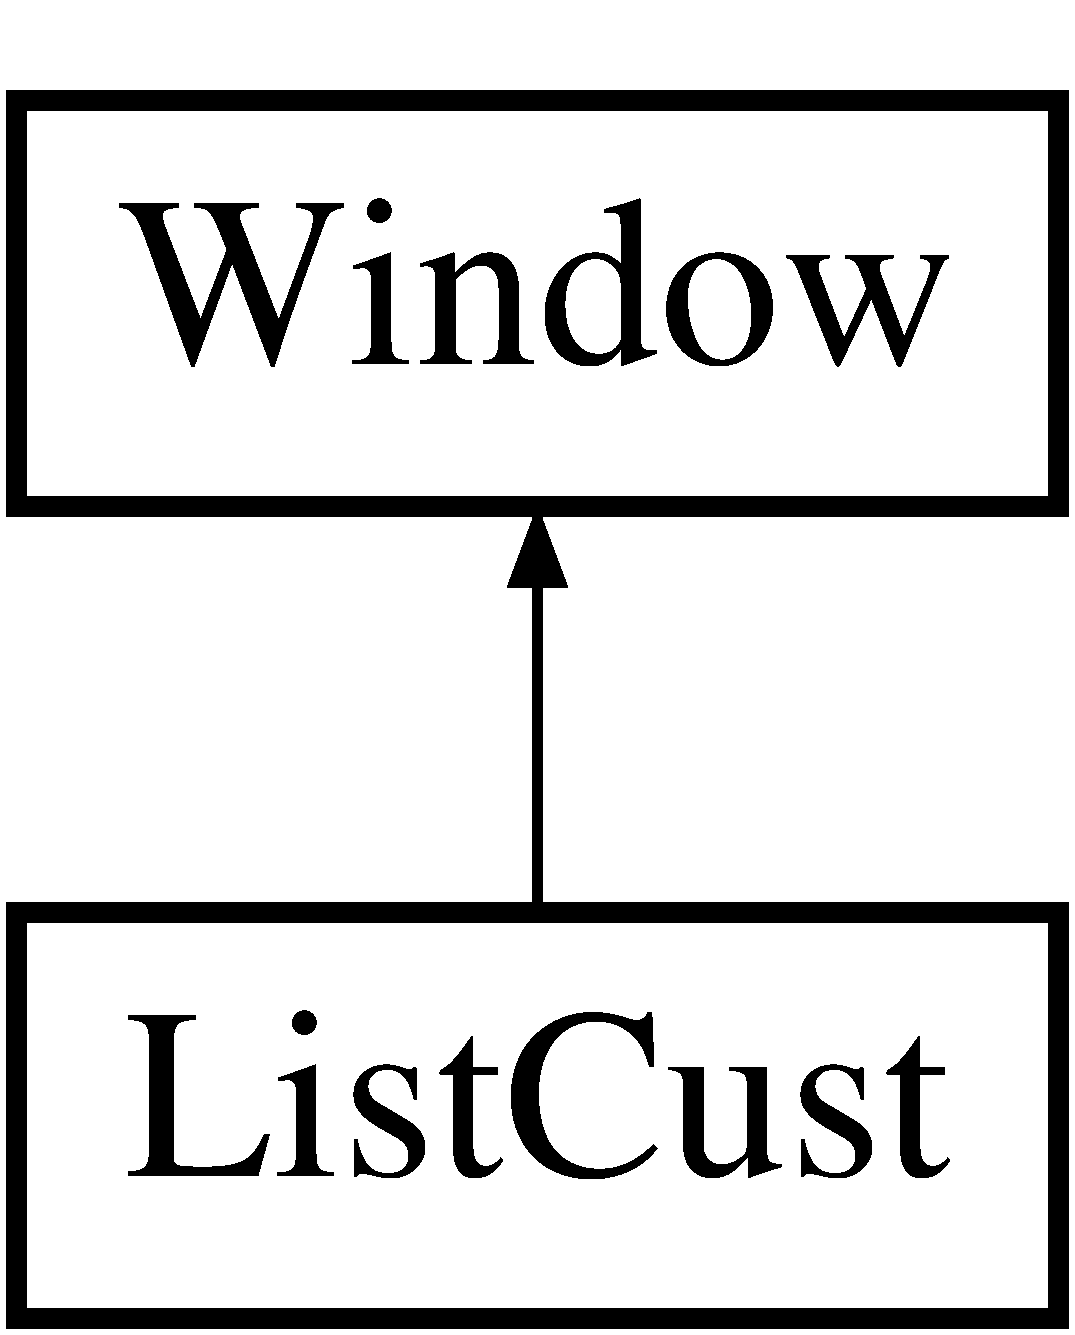
\includegraphics[height=2.000000cm]{classcustselect_1_1_list_cust}
\end{center}
\end{figure}
\subsection*{Public Member Functions}
\begin{DoxyCompactItemize}
\item 
def \hyperlink{classcustselect_1_1_list_cust_aeb833639525321c9d011dce1184c5d36}{\+\_\+\+\_\+init\+\_\+\+\_\+} (self, parent, \hyperlink{classcustselect_1_1_list_cust_a511ae0b1c13f95e5f08f1a0dd3da3d93}{data})
\item 
def \hyperlink{classcustselect_1_1_list_cust_a9e131589c1f888e8c69cc0a45796b78b}{fixed\+\_\+toggled} (self, cell, path, model)
\item 
def \hyperlink{classcustselect_1_1_list_cust_ade844b0d29257631707c9cf4374d65b2}{key\+\_\+press\+\_\+event} (self, win, event)
\item 
def \hyperlink{classcustselect_1_1_list_cust_ad22709b2e67308af35f55680d5a026e0}{run} (self)
\end{DoxyCompactItemize}
\subsection*{Data Fields}
\begin{DoxyCompactItemize}
\item 
\hyperlink{classcustselect_1_1_list_cust_a511ae0b1c13f95e5f08f1a0dd3da3d93}{data}
\item 
\hyperlink{classcustselect_1_1_list_cust_ab73fdaa1fb7669da760b49600c45d9be}{ok}
\end{DoxyCompactItemize}


\subsection{Constructor \& Destructor Documentation}
\mbox{\Hypertarget{classcustselect_1_1_list_cust_aeb833639525321c9d011dce1184c5d36}\label{classcustselect_1_1_list_cust_aeb833639525321c9d011dce1184c5d36}} 
\index{custselect\+::\+List\+Cust@{custselect\+::\+List\+Cust}!\+\_\+\+\_\+init\+\_\+\+\_\+@{\+\_\+\+\_\+init\+\_\+\+\_\+}}
\index{\+\_\+\+\_\+init\+\_\+\+\_\+@{\+\_\+\+\_\+init\+\_\+\+\_\+}!custselect\+::\+List\+Cust@{custselect\+::\+List\+Cust}}
\subsubsection{\texorpdfstring{\+\_\+\+\_\+init\+\_\+\+\_\+()}{\_\_init\_\_()}}
{\footnotesize\ttfamily def \+\_\+\+\_\+init\+\_\+\+\_\+ (\begin{DoxyParamCaption}\item[{}]{self,  }\item[{}]{parent,  }\item[{}]{data }\end{DoxyParamCaption})}



\subsection{Member Function Documentation}
\mbox{\Hypertarget{classcustselect_1_1_list_cust_a9e131589c1f888e8c69cc0a45796b78b}\label{classcustselect_1_1_list_cust_a9e131589c1f888e8c69cc0a45796b78b}} 
\index{custselect\+::\+List\+Cust@{custselect\+::\+List\+Cust}!fixed\+\_\+toggled@{fixed\+\_\+toggled}}
\index{fixed\+\_\+toggled@{fixed\+\_\+toggled}!custselect\+::\+List\+Cust@{custselect\+::\+List\+Cust}}
\subsubsection{\texorpdfstring{fixed\+\_\+toggled()}{fixed\_toggled()}}
{\footnotesize\ttfamily def fixed\+\_\+toggled (\begin{DoxyParamCaption}\item[{}]{self,  }\item[{}]{cell,  }\item[{}]{path,  }\item[{}]{model }\end{DoxyParamCaption})}

\mbox{\Hypertarget{classcustselect_1_1_list_cust_ade844b0d29257631707c9cf4374d65b2}\label{classcustselect_1_1_list_cust_ade844b0d29257631707c9cf4374d65b2}} 
\index{custselect\+::\+List\+Cust@{custselect\+::\+List\+Cust}!key\+\_\+press\+\_\+event@{key\+\_\+press\+\_\+event}}
\index{key\+\_\+press\+\_\+event@{key\+\_\+press\+\_\+event}!custselect\+::\+List\+Cust@{custselect\+::\+List\+Cust}}
\subsubsection{\texorpdfstring{key\+\_\+press\+\_\+event()}{key\_press\_event()}}
{\footnotesize\ttfamily def key\+\_\+press\+\_\+event (\begin{DoxyParamCaption}\item[{}]{self,  }\item[{}]{win,  }\item[{}]{event }\end{DoxyParamCaption})}

\mbox{\Hypertarget{classcustselect_1_1_list_cust_ad22709b2e67308af35f55680d5a026e0}\label{classcustselect_1_1_list_cust_ad22709b2e67308af35f55680d5a026e0}} 
\index{custselect\+::\+List\+Cust@{custselect\+::\+List\+Cust}!run@{run}}
\index{run@{run}!custselect\+::\+List\+Cust@{custselect\+::\+List\+Cust}}
\subsubsection{\texorpdfstring{run()}{run()}}
{\footnotesize\ttfamily def run (\begin{DoxyParamCaption}\item[{}]{self }\end{DoxyParamCaption})}



\subsection{Field Documentation}
\mbox{\Hypertarget{classcustselect_1_1_list_cust_a511ae0b1c13f95e5f08f1a0dd3da3d93}\label{classcustselect_1_1_list_cust_a511ae0b1c13f95e5f08f1a0dd3da3d93}} 
\index{custselect\+::\+List\+Cust@{custselect\+::\+List\+Cust}!data@{data}}
\index{data@{data}!custselect\+::\+List\+Cust@{custselect\+::\+List\+Cust}}
\subsubsection{\texorpdfstring{data}{data}}
{\footnotesize\ttfamily data}

\mbox{\Hypertarget{classcustselect_1_1_list_cust_ab73fdaa1fb7669da760b49600c45d9be}\label{classcustselect_1_1_list_cust_ab73fdaa1fb7669da760b49600c45d9be}} 
\index{custselect\+::\+List\+Cust@{custselect\+::\+List\+Cust}!ok@{ok}}
\index{ok@{ok}!custselect\+::\+List\+Cust@{custselect\+::\+List\+Cust}}
\subsubsection{\texorpdfstring{ok}{ok}}
{\footnotesize\ttfamily ok}



The documentation for this class was generated from the following file\+:\begin{DoxyCompactItemize}
\item 
gui/\hyperlink{custselect_8py}{custselect.\+py}\end{DoxyCompactItemize}

\hypertarget{classdibagui_1_1_main_win}{}\section{Main\+Win Class Reference}
\label{classdibagui_1_1_main_win}\index{Main\+Win@{Main\+Win}}
\subsection*{Public Member Functions}
\begin{DoxyCompactItemize}
\item 
def \hyperlink{classdibagui_1_1_main_win_ae64f0875afe3067b97ba370b354b9213}{\+\_\+\+\_\+init\+\_\+\+\_\+} (self)
\item 
def \hyperlink{classdibagui_1_1_main_win_a466c72a278968f797537b7bb3580f1b3}{imgbutt} (self, imgfile, txt, func, win)
\item 
def \hyperlink{classdibagui_1_1_main_win_a755988eaefd1fe0b4803b3eb4e22cf62}{exit\+\_\+all} (self, area=None, win=None)
\item 
def \hyperlink{classdibagui_1_1_main_win_ad1a61436bdc272bc9204e50462cfaadd}{next} (self, org)
\item 
def \hyperlink{classdibagui_1_1_main_win_a6a5b6d30b6cb3961e1f825b553f36b59}{transact} (self, area, me)
\item 
def \hyperlink{classdibagui_1_1_main_win_aa1be1965c9e4fba83ffe91fe97c3257b}{get\+\_\+one} (self, area, me)
\item 
def \hyperlink{classdibagui_1_1_main_win_a731892ba673be11c220b8d3306001be6}{show\+\_\+one} (self, area, me)
\item 
def \hyperlink{classdibagui_1_1_main_win_a385fd12b4740b087eb0e24ab6fa72396}{note\+\_\+focus\+\_\+in} (self, win, act)
\item 
def \hyperlink{classdibagui_1_1_main_win_a675dfb2de31ed3836c00bdc2545be10f}{note\+\_\+swpage\+\_\+cb} (self, tabx, page, num)
\item 
def \hyperlink{classdibagui_1_1_main_win_a5927791c4905069d5e2422577e5b9fa8}{del\+\_\+one} (self, area, me)
\item 
def \hyperlink{classdibagui_1_1_main_win_a4802385c549037f5813de35842fcbd55}{above\+\_\+one} (self, area, me)
\item 
def \hyperlink{classdibagui_1_1_main_win_ab2299ab818c9eb02e8307ca0fc41485b}{hide\+\_\+one} (self, area, me)
\item 
def \hyperlink{classdibagui_1_1_main_win_aa9e9c953cb53a8ab3cde7ec87464c67e}{done\+\_\+dlg} (self, dlg)
\item 
def \hyperlink{classdibagui_1_1_main_win_a6560530dba3370587c143736243793dc}{sel\+\_\+account} (self, area, me)
\item 
def \hyperlink{classdibagui_1_1_main_win_a56d6515e433aa4438622a3b3018913f5}{progress} (self, text)
\item 
def \hyperlink{classdibagui_1_1_main_win_a86a755556573728d23d3e706fb9341d9}{getkeyid} (self, fname)
\item 
def \hyperlink{classdibagui_1_1_main_win_ac2cede4bac22a589ebaae85651b77044}{unlink\+\_\+noerr} (self, fname)
\item 
def \hyperlink{classdibagui_1_1_main_win_a3006900cda7e6488b47296f3d0e420d3}{callback} (self, form)
\item 
def \hyperlink{classdibagui_1_1_main_win_ae455d2242af7dfc4e37c5db6f35e95fe}{new\+\_\+account} (self, area, me)
\item 
def \hyperlink{classdibagui_1_1_main_win_a5bbd1b5cae9e1e19a7ec7b2c1d48a834}{search} (self, area, me)
\item 
def \hyperlink{classdibagui_1_1_main_win_a0a399ceb2dc96ea47058aac94ae57047}{hide\+\_\+all} (self, area, me)
\item 
def \hyperlink{classdibagui_1_1_main_win_af4abcf75503c410e06d84af1a37909ea}{hide\+\_\+main} (self, area, me)
\item 
def \hyperlink{classdibagui_1_1_main_win_a260d37924dae7e20867bbd197b9044ee}{area\+\_\+button} (self, area, event)
\item 
def \hyperlink{classdibagui_1_1_main_win_a749f5e0497d5754e5c7800c8dc9d417c}{tree\+\_\+sel\+\_\+row} (self, xtree)
\item 
def \hyperlink{classdibagui_1_1_main_win_a7bb32848df24886f6972b780116052d2}{key\+\_\+press\+\_\+event} (self, area, event)
\item 
def \hyperlink{classdibagui_1_1_main_win_a41e1747cd5317f94dc683e74608bf7c6}{On\+Exit} (self, \hyperlink{namespacedibagui_a74b87337454200d4d33f80c4663dc5e5}{aa})
\item 
def \hyperlink{classdibagui_1_1_main_win_a22fab0ca18f0c6d3a657200fc3af5a52}{handler\+\_\+tick} (self)
\end{DoxyCompactItemize}
\subsection*{Data Fields}
\begin{DoxyCompactItemize}
\item 
\hyperlink{classdibagui_1_1_main_win_a1c3467ffffd2715943d16338156f1ef6}{timerx}
\item 
\hyperlink{classdibagui_1_1_main_win_a04a8a2bbfa9c15500892b8e5033d625b}{window}
\item 
\hyperlink{classdibagui_1_1_main_win_a9d9c279569f959f553951502d6a93194}{notebook}
\item 
\hyperlink{classdibagui_1_1_main_win_a76dbcfc78e812394f40977b0e13a3a47}{tree}
\item 
\hyperlink{classdibagui_1_1_main_win_a35543500c72c1c9eff1393f605e5ca10}{txt1}
\item 
\hyperlink{classdibagui_1_1_main_win_a3f3fcd00f4a6b97fbf9edcfa86d9607b}{account}
\item 
\hyperlink{classdibagui_1_1_main_win_a54f1d8208fc901f0d590d129e0fe4af7}{activity}
\item 
\hyperlink{classdibagui_1_1_main_win_a985893871a16e46a58441e60dc9da89f}{arr2}
\end{DoxyCompactItemize}


\subsection{Constructor \& Destructor Documentation}
\mbox{\Hypertarget{classdibagui_1_1_main_win_ae64f0875afe3067b97ba370b354b9213}\label{classdibagui_1_1_main_win_ae64f0875afe3067b97ba370b354b9213}} 
\index{dibagui\+::\+Main\+Win@{dibagui\+::\+Main\+Win}!\+\_\+\+\_\+init\+\_\+\+\_\+@{\+\_\+\+\_\+init\+\_\+\+\_\+}}
\index{\+\_\+\+\_\+init\+\_\+\+\_\+@{\+\_\+\+\_\+init\+\_\+\+\_\+}!dibagui\+::\+Main\+Win@{dibagui\+::\+Main\+Win}}
\subsubsection{\texorpdfstring{\+\_\+\+\_\+init\+\_\+\+\_\+()}{\_\_init\_\_()}}
{\footnotesize\ttfamily def \+\_\+\+\_\+init\+\_\+\+\_\+ (\begin{DoxyParamCaption}\item[{}]{self }\end{DoxyParamCaption})}



\subsection{Member Function Documentation}
\mbox{\Hypertarget{classdibagui_1_1_main_win_a4802385c549037f5813de35842fcbd55}\label{classdibagui_1_1_main_win_a4802385c549037f5813de35842fcbd55}} 
\index{dibagui\+::\+Main\+Win@{dibagui\+::\+Main\+Win}!above\+\_\+one@{above\+\_\+one}}
\index{above\+\_\+one@{above\+\_\+one}!dibagui\+::\+Main\+Win@{dibagui\+::\+Main\+Win}}
\subsubsection{\texorpdfstring{above\+\_\+one()}{above\_one()}}
{\footnotesize\ttfamily def above\+\_\+one (\begin{DoxyParamCaption}\item[{}]{self,  }\item[{}]{area,  }\item[{}]{me }\end{DoxyParamCaption})}

\mbox{\Hypertarget{classdibagui_1_1_main_win_a260d37924dae7e20867bbd197b9044ee}\label{classdibagui_1_1_main_win_a260d37924dae7e20867bbd197b9044ee}} 
\index{dibagui\+::\+Main\+Win@{dibagui\+::\+Main\+Win}!area\+\_\+button@{area\+\_\+button}}
\index{area\+\_\+button@{area\+\_\+button}!dibagui\+::\+Main\+Win@{dibagui\+::\+Main\+Win}}
\subsubsection{\texorpdfstring{area\+\_\+button()}{area\_button()}}
{\footnotesize\ttfamily def area\+\_\+button (\begin{DoxyParamCaption}\item[{}]{self,  }\item[{}]{area,  }\item[{}]{event }\end{DoxyParamCaption})}

\mbox{\Hypertarget{classdibagui_1_1_main_win_a3006900cda7e6488b47296f3d0e420d3}\label{classdibagui_1_1_main_win_a3006900cda7e6488b47296f3d0e420d3}} 
\index{dibagui\+::\+Main\+Win@{dibagui\+::\+Main\+Win}!callback@{callback}}
\index{callback@{callback}!dibagui\+::\+Main\+Win@{dibagui\+::\+Main\+Win}}
\subsubsection{\texorpdfstring{callback()}{callback()}}
{\footnotesize\ttfamily def callback (\begin{DoxyParamCaption}\item[{}]{self,  }\item[{}]{form }\end{DoxyParamCaption})}

\mbox{\Hypertarget{classdibagui_1_1_main_win_a5927791c4905069d5e2422577e5b9fa8}\label{classdibagui_1_1_main_win_a5927791c4905069d5e2422577e5b9fa8}} 
\index{dibagui\+::\+Main\+Win@{dibagui\+::\+Main\+Win}!del\+\_\+one@{del\+\_\+one}}
\index{del\+\_\+one@{del\+\_\+one}!dibagui\+::\+Main\+Win@{dibagui\+::\+Main\+Win}}
\subsubsection{\texorpdfstring{del\+\_\+one()}{del\_one()}}
{\footnotesize\ttfamily def del\+\_\+one (\begin{DoxyParamCaption}\item[{}]{self,  }\item[{}]{area,  }\item[{}]{me }\end{DoxyParamCaption})}

\mbox{\Hypertarget{classdibagui_1_1_main_win_aa9e9c953cb53a8ab3cde7ec87464c67e}\label{classdibagui_1_1_main_win_aa9e9c953cb53a8ab3cde7ec87464c67e}} 
\index{dibagui\+::\+Main\+Win@{dibagui\+::\+Main\+Win}!done\+\_\+dlg@{done\+\_\+dlg}}
\index{done\+\_\+dlg@{done\+\_\+dlg}!dibagui\+::\+Main\+Win@{dibagui\+::\+Main\+Win}}
\subsubsection{\texorpdfstring{done\+\_\+dlg()}{done\_dlg()}}
{\footnotesize\ttfamily def done\+\_\+dlg (\begin{DoxyParamCaption}\item[{}]{self,  }\item[{}]{dlg }\end{DoxyParamCaption})}

\mbox{\Hypertarget{classdibagui_1_1_main_win_a755988eaefd1fe0b4803b3eb4e22cf62}\label{classdibagui_1_1_main_win_a755988eaefd1fe0b4803b3eb4e22cf62}} 
\index{dibagui\+::\+Main\+Win@{dibagui\+::\+Main\+Win}!exit\+\_\+all@{exit\+\_\+all}}
\index{exit\+\_\+all@{exit\+\_\+all}!dibagui\+::\+Main\+Win@{dibagui\+::\+Main\+Win}}
\subsubsection{\texorpdfstring{exit\+\_\+all()}{exit\_all()}}
{\footnotesize\ttfamily def exit\+\_\+all (\begin{DoxyParamCaption}\item[{}]{self,  }\item[{}]{area = {\ttfamily None},  }\item[{}]{win = {\ttfamily None} }\end{DoxyParamCaption})}

\mbox{\Hypertarget{classdibagui_1_1_main_win_aa1be1965c9e4fba83ffe91fe97c3257b}\label{classdibagui_1_1_main_win_aa1be1965c9e4fba83ffe91fe97c3257b}} 
\index{dibagui\+::\+Main\+Win@{dibagui\+::\+Main\+Win}!get\+\_\+one@{get\+\_\+one}}
\index{get\+\_\+one@{get\+\_\+one}!dibagui\+::\+Main\+Win@{dibagui\+::\+Main\+Win}}
\subsubsection{\texorpdfstring{get\+\_\+one()}{get\_one()}}
{\footnotesize\ttfamily def get\+\_\+one (\begin{DoxyParamCaption}\item[{}]{self,  }\item[{}]{area,  }\item[{}]{me }\end{DoxyParamCaption})}

\mbox{\Hypertarget{classdibagui_1_1_main_win_a86a755556573728d23d3e706fb9341d9}\label{classdibagui_1_1_main_win_a86a755556573728d23d3e706fb9341d9}} 
\index{dibagui\+::\+Main\+Win@{dibagui\+::\+Main\+Win}!getkeyid@{getkeyid}}
\index{getkeyid@{getkeyid}!dibagui\+::\+Main\+Win@{dibagui\+::\+Main\+Win}}
\subsubsection{\texorpdfstring{getkeyid()}{getkeyid()}}
{\footnotesize\ttfamily def getkeyid (\begin{DoxyParamCaption}\item[{}]{self,  }\item[{}]{fname }\end{DoxyParamCaption})}

\mbox{\Hypertarget{classdibagui_1_1_main_win_a22fab0ca18f0c6d3a657200fc3af5a52}\label{classdibagui_1_1_main_win_a22fab0ca18f0c6d3a657200fc3af5a52}} 
\index{dibagui\+::\+Main\+Win@{dibagui\+::\+Main\+Win}!handler\+\_\+tick@{handler\+\_\+tick}}
\index{handler\+\_\+tick@{handler\+\_\+tick}!dibagui\+::\+Main\+Win@{dibagui\+::\+Main\+Win}}
\subsubsection{\texorpdfstring{handler\+\_\+tick()}{handler\_tick()}}
{\footnotesize\ttfamily def handler\+\_\+tick (\begin{DoxyParamCaption}\item[{}]{self }\end{DoxyParamCaption})}

\mbox{\Hypertarget{classdibagui_1_1_main_win_a0a399ceb2dc96ea47058aac94ae57047}\label{classdibagui_1_1_main_win_a0a399ceb2dc96ea47058aac94ae57047}} 
\index{dibagui\+::\+Main\+Win@{dibagui\+::\+Main\+Win}!hide\+\_\+all@{hide\+\_\+all}}
\index{hide\+\_\+all@{hide\+\_\+all}!dibagui\+::\+Main\+Win@{dibagui\+::\+Main\+Win}}
\subsubsection{\texorpdfstring{hide\+\_\+all()}{hide\_all()}}
{\footnotesize\ttfamily def hide\+\_\+all (\begin{DoxyParamCaption}\item[{}]{self,  }\item[{}]{area,  }\item[{}]{me }\end{DoxyParamCaption})}

\mbox{\Hypertarget{classdibagui_1_1_main_win_af4abcf75503c410e06d84af1a37909ea}\label{classdibagui_1_1_main_win_af4abcf75503c410e06d84af1a37909ea}} 
\index{dibagui\+::\+Main\+Win@{dibagui\+::\+Main\+Win}!hide\+\_\+main@{hide\+\_\+main}}
\index{hide\+\_\+main@{hide\+\_\+main}!dibagui\+::\+Main\+Win@{dibagui\+::\+Main\+Win}}
\subsubsection{\texorpdfstring{hide\+\_\+main()}{hide\_main()}}
{\footnotesize\ttfamily def hide\+\_\+main (\begin{DoxyParamCaption}\item[{}]{self,  }\item[{}]{area,  }\item[{}]{me }\end{DoxyParamCaption})}

\mbox{\Hypertarget{classdibagui_1_1_main_win_ab2299ab818c9eb02e8307ca0fc41485b}\label{classdibagui_1_1_main_win_ab2299ab818c9eb02e8307ca0fc41485b}} 
\index{dibagui\+::\+Main\+Win@{dibagui\+::\+Main\+Win}!hide\+\_\+one@{hide\+\_\+one}}
\index{hide\+\_\+one@{hide\+\_\+one}!dibagui\+::\+Main\+Win@{dibagui\+::\+Main\+Win}}
\subsubsection{\texorpdfstring{hide\+\_\+one()}{hide\_one()}}
{\footnotesize\ttfamily def hide\+\_\+one (\begin{DoxyParamCaption}\item[{}]{self,  }\item[{}]{area,  }\item[{}]{me }\end{DoxyParamCaption})}

\mbox{\Hypertarget{classdibagui_1_1_main_win_a466c72a278968f797537b7bb3580f1b3}\label{classdibagui_1_1_main_win_a466c72a278968f797537b7bb3580f1b3}} 
\index{dibagui\+::\+Main\+Win@{dibagui\+::\+Main\+Win}!imgbutt@{imgbutt}}
\index{imgbutt@{imgbutt}!dibagui\+::\+Main\+Win@{dibagui\+::\+Main\+Win}}
\subsubsection{\texorpdfstring{imgbutt()}{imgbutt()}}
{\footnotesize\ttfamily def imgbutt (\begin{DoxyParamCaption}\item[{}]{self,  }\item[{}]{imgfile,  }\item[{}]{txt,  }\item[{}]{func,  }\item[{}]{win }\end{DoxyParamCaption})}

\mbox{\Hypertarget{classdibagui_1_1_main_win_a7bb32848df24886f6972b780116052d2}\label{classdibagui_1_1_main_win_a7bb32848df24886f6972b780116052d2}} 
\index{dibagui\+::\+Main\+Win@{dibagui\+::\+Main\+Win}!key\+\_\+press\+\_\+event@{key\+\_\+press\+\_\+event}}
\index{key\+\_\+press\+\_\+event@{key\+\_\+press\+\_\+event}!dibagui\+::\+Main\+Win@{dibagui\+::\+Main\+Win}}
\subsubsection{\texorpdfstring{key\+\_\+press\+\_\+event()}{key\_press\_event()}}
{\footnotesize\ttfamily def key\+\_\+press\+\_\+event (\begin{DoxyParamCaption}\item[{}]{self,  }\item[{}]{area,  }\item[{}]{event }\end{DoxyParamCaption})}

\mbox{\Hypertarget{classdibagui_1_1_main_win_ae455d2242af7dfc4e37c5db6f35e95fe}\label{classdibagui_1_1_main_win_ae455d2242af7dfc4e37c5db6f35e95fe}} 
\index{dibagui\+::\+Main\+Win@{dibagui\+::\+Main\+Win}!new\+\_\+account@{new\+\_\+account}}
\index{new\+\_\+account@{new\+\_\+account}!dibagui\+::\+Main\+Win@{dibagui\+::\+Main\+Win}}
\subsubsection{\texorpdfstring{new\+\_\+account()}{new\_account()}}
{\footnotesize\ttfamily def new\+\_\+account (\begin{DoxyParamCaption}\item[{}]{self,  }\item[{}]{area,  }\item[{}]{me }\end{DoxyParamCaption})}

\mbox{\Hypertarget{classdibagui_1_1_main_win_ad1a61436bdc272bc9204e50462cfaadd}\label{classdibagui_1_1_main_win_ad1a61436bdc272bc9204e50462cfaadd}} 
\index{dibagui\+::\+Main\+Win@{dibagui\+::\+Main\+Win}!next@{next}}
\index{next@{next}!dibagui\+::\+Main\+Win@{dibagui\+::\+Main\+Win}}
\subsubsection{\texorpdfstring{next()}{next()}}
{\footnotesize\ttfamily def next (\begin{DoxyParamCaption}\item[{}]{self,  }\item[{}]{org }\end{DoxyParamCaption})}

\mbox{\Hypertarget{classdibagui_1_1_main_win_a385fd12b4740b087eb0e24ab6fa72396}\label{classdibagui_1_1_main_win_a385fd12b4740b087eb0e24ab6fa72396}} 
\index{dibagui\+::\+Main\+Win@{dibagui\+::\+Main\+Win}!note\+\_\+focus\+\_\+in@{note\+\_\+focus\+\_\+in}}
\index{note\+\_\+focus\+\_\+in@{note\+\_\+focus\+\_\+in}!dibagui\+::\+Main\+Win@{dibagui\+::\+Main\+Win}}
\subsubsection{\texorpdfstring{note\+\_\+focus\+\_\+in()}{note\_focus\_in()}}
{\footnotesize\ttfamily def note\+\_\+focus\+\_\+in (\begin{DoxyParamCaption}\item[{}]{self,  }\item[{}]{win,  }\item[{}]{act }\end{DoxyParamCaption})}

\mbox{\Hypertarget{classdibagui_1_1_main_win_a675dfb2de31ed3836c00bdc2545be10f}\label{classdibagui_1_1_main_win_a675dfb2de31ed3836c00bdc2545be10f}} 
\index{dibagui\+::\+Main\+Win@{dibagui\+::\+Main\+Win}!note\+\_\+swpage\+\_\+cb@{note\+\_\+swpage\+\_\+cb}}
\index{note\+\_\+swpage\+\_\+cb@{note\+\_\+swpage\+\_\+cb}!dibagui\+::\+Main\+Win@{dibagui\+::\+Main\+Win}}
\subsubsection{\texorpdfstring{note\+\_\+swpage\+\_\+cb()}{note\_swpage\_cb()}}
{\footnotesize\ttfamily def note\+\_\+swpage\+\_\+cb (\begin{DoxyParamCaption}\item[{}]{self,  }\item[{}]{tabx,  }\item[{}]{page,  }\item[{}]{num }\end{DoxyParamCaption})}

\mbox{\Hypertarget{classdibagui_1_1_main_win_a41e1747cd5317f94dc683e74608bf7c6}\label{classdibagui_1_1_main_win_a41e1747cd5317f94dc683e74608bf7c6}} 
\index{dibagui\+::\+Main\+Win@{dibagui\+::\+Main\+Win}!On\+Exit@{On\+Exit}}
\index{On\+Exit@{On\+Exit}!dibagui\+::\+Main\+Win@{dibagui\+::\+Main\+Win}}
\subsubsection{\texorpdfstring{On\+Exit()}{OnExit()}}
{\footnotesize\ttfamily def On\+Exit (\begin{DoxyParamCaption}\item[{}]{self,  }\item[{}]{aa }\end{DoxyParamCaption})}

\mbox{\Hypertarget{classdibagui_1_1_main_win_a56d6515e433aa4438622a3b3018913f5}\label{classdibagui_1_1_main_win_a56d6515e433aa4438622a3b3018913f5}} 
\index{dibagui\+::\+Main\+Win@{dibagui\+::\+Main\+Win}!progress@{progress}}
\index{progress@{progress}!dibagui\+::\+Main\+Win@{dibagui\+::\+Main\+Win}}
\subsubsection{\texorpdfstring{progress()}{progress()}}
{\footnotesize\ttfamily def progress (\begin{DoxyParamCaption}\item[{}]{self,  }\item[{}]{text }\end{DoxyParamCaption})}

\mbox{\Hypertarget{classdibagui_1_1_main_win_a5bbd1b5cae9e1e19a7ec7b2c1d48a834}\label{classdibagui_1_1_main_win_a5bbd1b5cae9e1e19a7ec7b2c1d48a834}} 
\index{dibagui\+::\+Main\+Win@{dibagui\+::\+Main\+Win}!search@{search}}
\index{search@{search}!dibagui\+::\+Main\+Win@{dibagui\+::\+Main\+Win}}
\subsubsection{\texorpdfstring{search()}{search()}}
{\footnotesize\ttfamily def search (\begin{DoxyParamCaption}\item[{}]{self,  }\item[{}]{area,  }\item[{}]{me }\end{DoxyParamCaption})}

\mbox{\Hypertarget{classdibagui_1_1_main_win_a6560530dba3370587c143736243793dc}\label{classdibagui_1_1_main_win_a6560530dba3370587c143736243793dc}} 
\index{dibagui\+::\+Main\+Win@{dibagui\+::\+Main\+Win}!sel\+\_\+account@{sel\+\_\+account}}
\index{sel\+\_\+account@{sel\+\_\+account}!dibagui\+::\+Main\+Win@{dibagui\+::\+Main\+Win}}
\subsubsection{\texorpdfstring{sel\+\_\+account()}{sel\_account()}}
{\footnotesize\ttfamily def sel\+\_\+account (\begin{DoxyParamCaption}\item[{}]{self,  }\item[{}]{area,  }\item[{}]{me }\end{DoxyParamCaption})}

\mbox{\Hypertarget{classdibagui_1_1_main_win_a731892ba673be11c220b8d3306001be6}\label{classdibagui_1_1_main_win_a731892ba673be11c220b8d3306001be6}} 
\index{dibagui\+::\+Main\+Win@{dibagui\+::\+Main\+Win}!show\+\_\+one@{show\+\_\+one}}
\index{show\+\_\+one@{show\+\_\+one}!dibagui\+::\+Main\+Win@{dibagui\+::\+Main\+Win}}
\subsubsection{\texorpdfstring{show\+\_\+one()}{show\_one()}}
{\footnotesize\ttfamily def show\+\_\+one (\begin{DoxyParamCaption}\item[{}]{self,  }\item[{}]{area,  }\item[{}]{me }\end{DoxyParamCaption})}

\mbox{\Hypertarget{classdibagui_1_1_main_win_a6a5b6d30b6cb3961e1f825b553f36b59}\label{classdibagui_1_1_main_win_a6a5b6d30b6cb3961e1f825b553f36b59}} 
\index{dibagui\+::\+Main\+Win@{dibagui\+::\+Main\+Win}!transact@{transact}}
\index{transact@{transact}!dibagui\+::\+Main\+Win@{dibagui\+::\+Main\+Win}}
\subsubsection{\texorpdfstring{transact()}{transact()}}
{\footnotesize\ttfamily def transact (\begin{DoxyParamCaption}\item[{}]{self,  }\item[{}]{area,  }\item[{}]{me }\end{DoxyParamCaption})}

\mbox{\Hypertarget{classdibagui_1_1_main_win_a749f5e0497d5754e5c7800c8dc9d417c}\label{classdibagui_1_1_main_win_a749f5e0497d5754e5c7800c8dc9d417c}} 
\index{dibagui\+::\+Main\+Win@{dibagui\+::\+Main\+Win}!tree\+\_\+sel\+\_\+row@{tree\+\_\+sel\+\_\+row}}
\index{tree\+\_\+sel\+\_\+row@{tree\+\_\+sel\+\_\+row}!dibagui\+::\+Main\+Win@{dibagui\+::\+Main\+Win}}
\subsubsection{\texorpdfstring{tree\+\_\+sel\+\_\+row()}{tree\_sel\_row()}}
{\footnotesize\ttfamily def tree\+\_\+sel\+\_\+row (\begin{DoxyParamCaption}\item[{}]{self,  }\item[{}]{xtree }\end{DoxyParamCaption})}

\mbox{\Hypertarget{classdibagui_1_1_main_win_ac2cede4bac22a589ebaae85651b77044}\label{classdibagui_1_1_main_win_ac2cede4bac22a589ebaae85651b77044}} 
\index{dibagui\+::\+Main\+Win@{dibagui\+::\+Main\+Win}!unlink\+\_\+noerr@{unlink\+\_\+noerr}}
\index{unlink\+\_\+noerr@{unlink\+\_\+noerr}!dibagui\+::\+Main\+Win@{dibagui\+::\+Main\+Win}}
\subsubsection{\texorpdfstring{unlink\+\_\+noerr()}{unlink\_noerr()}}
{\footnotesize\ttfamily def unlink\+\_\+noerr (\begin{DoxyParamCaption}\item[{}]{self,  }\item[{}]{fname }\end{DoxyParamCaption})}



\subsection{Field Documentation}
\mbox{\Hypertarget{classdibagui_1_1_main_win_a3f3fcd00f4a6b97fbf9edcfa86d9607b}\label{classdibagui_1_1_main_win_a3f3fcd00f4a6b97fbf9edcfa86d9607b}} 
\index{dibagui\+::\+Main\+Win@{dibagui\+::\+Main\+Win}!account@{account}}
\index{account@{account}!dibagui\+::\+Main\+Win@{dibagui\+::\+Main\+Win}}
\subsubsection{\texorpdfstring{account}{account}}
{\footnotesize\ttfamily account}

\mbox{\Hypertarget{classdibagui_1_1_main_win_a54f1d8208fc901f0d590d129e0fe4af7}\label{classdibagui_1_1_main_win_a54f1d8208fc901f0d590d129e0fe4af7}} 
\index{dibagui\+::\+Main\+Win@{dibagui\+::\+Main\+Win}!activity@{activity}}
\index{activity@{activity}!dibagui\+::\+Main\+Win@{dibagui\+::\+Main\+Win}}
\subsubsection{\texorpdfstring{activity}{activity}}
{\footnotesize\ttfamily activity}

\mbox{\Hypertarget{classdibagui_1_1_main_win_a985893871a16e46a58441e60dc9da89f}\label{classdibagui_1_1_main_win_a985893871a16e46a58441e60dc9da89f}} 
\index{dibagui\+::\+Main\+Win@{dibagui\+::\+Main\+Win}!arr2@{arr2}}
\index{arr2@{arr2}!dibagui\+::\+Main\+Win@{dibagui\+::\+Main\+Win}}
\subsubsection{\texorpdfstring{arr2}{arr2}}
{\footnotesize\ttfamily arr2}

\mbox{\Hypertarget{classdibagui_1_1_main_win_a9d9c279569f959f553951502d6a93194}\label{classdibagui_1_1_main_win_a9d9c279569f959f553951502d6a93194}} 
\index{dibagui\+::\+Main\+Win@{dibagui\+::\+Main\+Win}!notebook@{notebook}}
\index{notebook@{notebook}!dibagui\+::\+Main\+Win@{dibagui\+::\+Main\+Win}}
\subsubsection{\texorpdfstring{notebook}{notebook}}
{\footnotesize\ttfamily notebook}

\mbox{\Hypertarget{classdibagui_1_1_main_win_a1c3467ffffd2715943d16338156f1ef6}\label{classdibagui_1_1_main_win_a1c3467ffffd2715943d16338156f1ef6}} 
\index{dibagui\+::\+Main\+Win@{dibagui\+::\+Main\+Win}!timerx@{timerx}}
\index{timerx@{timerx}!dibagui\+::\+Main\+Win@{dibagui\+::\+Main\+Win}}
\subsubsection{\texorpdfstring{timerx}{timerx}}
{\footnotesize\ttfamily timerx}

\mbox{\Hypertarget{classdibagui_1_1_main_win_a76dbcfc78e812394f40977b0e13a3a47}\label{classdibagui_1_1_main_win_a76dbcfc78e812394f40977b0e13a3a47}} 
\index{dibagui\+::\+Main\+Win@{dibagui\+::\+Main\+Win}!tree@{tree}}
\index{tree@{tree}!dibagui\+::\+Main\+Win@{dibagui\+::\+Main\+Win}}
\subsubsection{\texorpdfstring{tree}{tree}}
{\footnotesize\ttfamily tree}

\mbox{\Hypertarget{classdibagui_1_1_main_win_a35543500c72c1c9eff1393f605e5ca10}\label{classdibagui_1_1_main_win_a35543500c72c1c9eff1393f605e5ca10}} 
\index{dibagui\+::\+Main\+Win@{dibagui\+::\+Main\+Win}!txt1@{txt1}}
\index{txt1@{txt1}!dibagui\+::\+Main\+Win@{dibagui\+::\+Main\+Win}}
\subsubsection{\texorpdfstring{txt1}{txt1}}
{\footnotesize\ttfamily txt1}

\mbox{\Hypertarget{classdibagui_1_1_main_win_a04a8a2bbfa9c15500892b8e5033d625b}\label{classdibagui_1_1_main_win_a04a8a2bbfa9c15500892b8e5033d625b}} 
\index{dibagui\+::\+Main\+Win@{dibagui\+::\+Main\+Win}!window@{window}}
\index{window@{window}!dibagui\+::\+Main\+Win@{dibagui\+::\+Main\+Win}}
\subsubsection{\texorpdfstring{window}{window}}
{\footnotesize\ttfamily window}



The documentation for this class was generated from the following file\+:\begin{DoxyCompactItemize}
\item 
gui/\hyperlink{dibagui_8py}{dibagui.\+py}\end{DoxyCompactItemize}

\hypertarget{classnewcust_1_1_new_cust}{}\section{New\+Cust Class Reference}
\label{classnewcust_1_1_new_cust}\index{New\+Cust@{New\+Cust}}
Inheritance diagram for New\+Cust\+:\begin{figure}[H]
\begin{center}
\leavevmode
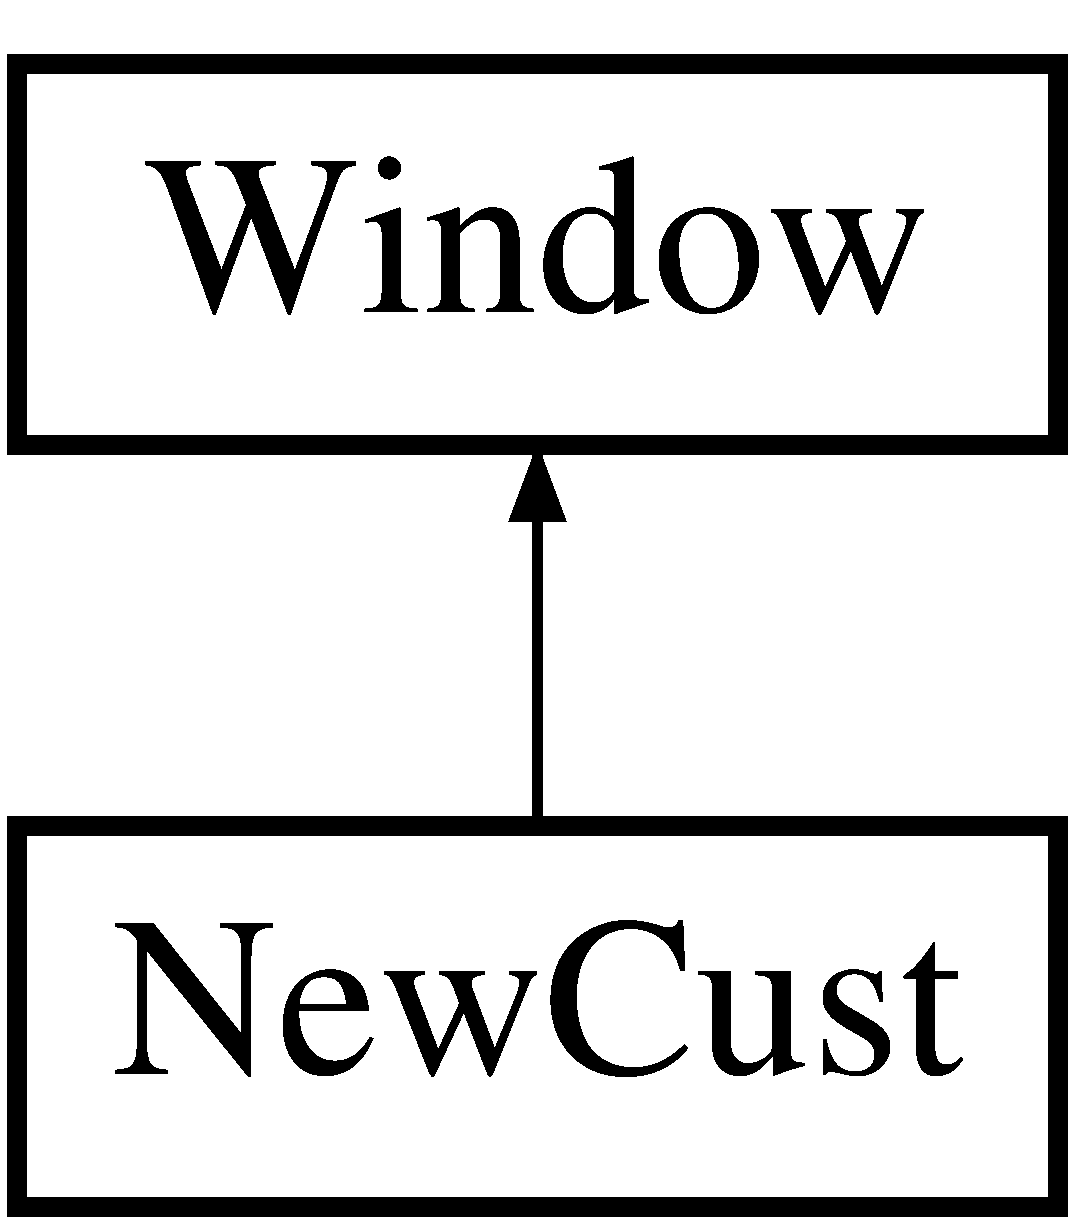
\includegraphics[height=2.000000cm]{classnewcust_1_1_new_cust}
\end{center}
\end{figure}
\subsection*{Public Member Functions}
\begin{DoxyCompactItemize}
\item 
def \hyperlink{classnewcust_1_1_new_cust_a6525fc41c20a15b5679d6c1b25ed6382}{\+\_\+\+\_\+init\+\_\+\+\_\+} (self, par, \hyperlink{classnewcust_1_1_new_cust_a599b5ba47e46802f9612991a1671b10d}{cback}, uuid\+\_\+name, datax=None)
\item 
def \hyperlink{classnewcust_1_1_new_cust_ad22709b2e67308af35f55680d5a026e0}{run} (self)
\item 
def \hyperlink{classnewcust_1_1_new_cust_a90898fd7a9cd186cdf5049af48358987}{spacer} (self, hbox, xstr=\char`\"{}    \char`\"{}, expand=False)
\item 
def \hyperlink{classnewcust_1_1_new_cust_a0dac401bad64932c202b80373a8b8204}{vspacer} (self, vbox, xstr=\char`\"{}     \char`\"{}, expand=False)
\item 
def \hyperlink{classnewcust_1_1_new_cust_a52808e81a3a13f8152d1915c83f101ae}{click\+\_\+ok} (self, butt, xx)
\item 
def \hyperlink{classnewcust_1_1_new_cust_a2340f5763bb2cb8bb86f00d1f7af196c}{click\+\_\+can} (self, butt, xx)
\item 
def \hyperlink{classnewcust_1_1_new_cust_ade844b0d29257631707c9cf4374d65b2}{key\+\_\+press\+\_\+event} (self, win, event)
\item 
def \hyperlink{classnewcust_1_1_new_cust_ac8f0164ed23b47c62b9bf93f8dfddba8}{area\+\_\+button} (self, butt)
\item 
def \hyperlink{classnewcust_1_1_new_cust_a44d5d34e5cf3202869ac1d4c4a991506}{scrolledtext} (self, name, body=None)
\item 
def \hyperlink{classnewcust_1_1_new_cust_aa439dd5761c7e8e65f3d333652744af9}{entryquad} (self, vbox, entry1, entry2)
\item 
def \hyperlink{classnewcust_1_1_new_cust_a7c7269fccea3b838ca0c7580277ef8d9}{entrypair} (self, vbox, labtext, labname, tip, defval=None)
\item 
def \hyperlink{classnewcust_1_1_new_cust_ab063a0c78082406f614cdd9aaef1531f}{textviewpair} (self, vbox, labtext, labname, tip, defval=None)
\item 
def \hyperlink{classnewcust_1_1_new_cust_a22fab0ca18f0c6d3a657200fc3af5a52}{handler\+\_\+tick} (self)
\end{DoxyCompactItemize}
\subsection*{Data Fields}
\begin{DoxyCompactItemize}
\item 
\hyperlink{classnewcust_1_1_new_cust_a599b5ba47e46802f9612991a1671b10d}{cback}
\item 
\hyperlink{classnewcust_1_1_new_cust_ab73fdaa1fb7669da760b49600c45d9be}{ok}
\item 
\hyperlink{classnewcust_1_1_new_cust_a6315dfe6e05d2814c94e9eb9a5eab999}{arr}
\end{DoxyCompactItemize}


\subsection{Constructor \& Destructor Documentation}
\mbox{\Hypertarget{classnewcust_1_1_new_cust_a6525fc41c20a15b5679d6c1b25ed6382}\label{classnewcust_1_1_new_cust_a6525fc41c20a15b5679d6c1b25ed6382}} 
\index{newcust\+::\+New\+Cust@{newcust\+::\+New\+Cust}!\+\_\+\+\_\+init\+\_\+\+\_\+@{\+\_\+\+\_\+init\+\_\+\+\_\+}}
\index{\+\_\+\+\_\+init\+\_\+\+\_\+@{\+\_\+\+\_\+init\+\_\+\+\_\+}!newcust\+::\+New\+Cust@{newcust\+::\+New\+Cust}}
\subsubsection{\texorpdfstring{\+\_\+\+\_\+init\+\_\+\+\_\+()}{\_\_init\_\_()}}
{\footnotesize\ttfamily def \+\_\+\+\_\+init\+\_\+\+\_\+ (\begin{DoxyParamCaption}\item[{}]{self,  }\item[{}]{par,  }\item[{}]{cback,  }\item[{}]{uuid\+\_\+name,  }\item[{}]{datax = {\ttfamily None} }\end{DoxyParamCaption})}



\subsection{Member Function Documentation}
\mbox{\Hypertarget{classnewcust_1_1_new_cust_ac8f0164ed23b47c62b9bf93f8dfddba8}\label{classnewcust_1_1_new_cust_ac8f0164ed23b47c62b9bf93f8dfddba8}} 
\index{newcust\+::\+New\+Cust@{newcust\+::\+New\+Cust}!area\+\_\+button@{area\+\_\+button}}
\index{area\+\_\+button@{area\+\_\+button}!newcust\+::\+New\+Cust@{newcust\+::\+New\+Cust}}
\subsubsection{\texorpdfstring{area\+\_\+button()}{area\_button()}}
{\footnotesize\ttfamily def area\+\_\+button (\begin{DoxyParamCaption}\item[{}]{self,  }\item[{}]{butt }\end{DoxyParamCaption})}

\mbox{\Hypertarget{classnewcust_1_1_new_cust_a2340f5763bb2cb8bb86f00d1f7af196c}\label{classnewcust_1_1_new_cust_a2340f5763bb2cb8bb86f00d1f7af196c}} 
\index{newcust\+::\+New\+Cust@{newcust\+::\+New\+Cust}!click\+\_\+can@{click\+\_\+can}}
\index{click\+\_\+can@{click\+\_\+can}!newcust\+::\+New\+Cust@{newcust\+::\+New\+Cust}}
\subsubsection{\texorpdfstring{click\+\_\+can()}{click\_can()}}
{\footnotesize\ttfamily def click\+\_\+can (\begin{DoxyParamCaption}\item[{}]{self,  }\item[{}]{butt,  }\item[{}]{xx }\end{DoxyParamCaption})}

\mbox{\Hypertarget{classnewcust_1_1_new_cust_a52808e81a3a13f8152d1915c83f101ae}\label{classnewcust_1_1_new_cust_a52808e81a3a13f8152d1915c83f101ae}} 
\index{newcust\+::\+New\+Cust@{newcust\+::\+New\+Cust}!click\+\_\+ok@{click\+\_\+ok}}
\index{click\+\_\+ok@{click\+\_\+ok}!newcust\+::\+New\+Cust@{newcust\+::\+New\+Cust}}
\subsubsection{\texorpdfstring{click\+\_\+ok()}{click\_ok()}}
{\footnotesize\ttfamily def click\+\_\+ok (\begin{DoxyParamCaption}\item[{}]{self,  }\item[{}]{butt,  }\item[{}]{xx }\end{DoxyParamCaption})}

\mbox{\Hypertarget{classnewcust_1_1_new_cust_a7c7269fccea3b838ca0c7580277ef8d9}\label{classnewcust_1_1_new_cust_a7c7269fccea3b838ca0c7580277ef8d9}} 
\index{newcust\+::\+New\+Cust@{newcust\+::\+New\+Cust}!entrypair@{entrypair}}
\index{entrypair@{entrypair}!newcust\+::\+New\+Cust@{newcust\+::\+New\+Cust}}
\subsubsection{\texorpdfstring{entrypair()}{entrypair()}}
{\footnotesize\ttfamily def entrypair (\begin{DoxyParamCaption}\item[{}]{self,  }\item[{}]{vbox,  }\item[{}]{labtext,  }\item[{}]{labname,  }\item[{}]{tip,  }\item[{}]{defval = {\ttfamily None} }\end{DoxyParamCaption})}

\mbox{\Hypertarget{classnewcust_1_1_new_cust_aa439dd5761c7e8e65f3d333652744af9}\label{classnewcust_1_1_new_cust_aa439dd5761c7e8e65f3d333652744af9}} 
\index{newcust\+::\+New\+Cust@{newcust\+::\+New\+Cust}!entryquad@{entryquad}}
\index{entryquad@{entryquad}!newcust\+::\+New\+Cust@{newcust\+::\+New\+Cust}}
\subsubsection{\texorpdfstring{entryquad()}{entryquad()}}
{\footnotesize\ttfamily def entryquad (\begin{DoxyParamCaption}\item[{}]{self,  }\item[{}]{vbox,  }\item[{}]{entry1,  }\item[{}]{entry2 }\end{DoxyParamCaption})}

\mbox{\Hypertarget{classnewcust_1_1_new_cust_a22fab0ca18f0c6d3a657200fc3af5a52}\label{classnewcust_1_1_new_cust_a22fab0ca18f0c6d3a657200fc3af5a52}} 
\index{newcust\+::\+New\+Cust@{newcust\+::\+New\+Cust}!handler\+\_\+tick@{handler\+\_\+tick}}
\index{handler\+\_\+tick@{handler\+\_\+tick}!newcust\+::\+New\+Cust@{newcust\+::\+New\+Cust}}
\subsubsection{\texorpdfstring{handler\+\_\+tick()}{handler\_tick()}}
{\footnotesize\ttfamily def handler\+\_\+tick (\begin{DoxyParamCaption}\item[{}]{self }\end{DoxyParamCaption})}

\mbox{\Hypertarget{classnewcust_1_1_new_cust_ade844b0d29257631707c9cf4374d65b2}\label{classnewcust_1_1_new_cust_ade844b0d29257631707c9cf4374d65b2}} 
\index{newcust\+::\+New\+Cust@{newcust\+::\+New\+Cust}!key\+\_\+press\+\_\+event@{key\+\_\+press\+\_\+event}}
\index{key\+\_\+press\+\_\+event@{key\+\_\+press\+\_\+event}!newcust\+::\+New\+Cust@{newcust\+::\+New\+Cust}}
\subsubsection{\texorpdfstring{key\+\_\+press\+\_\+event()}{key\_press\_event()}}
{\footnotesize\ttfamily def key\+\_\+press\+\_\+event (\begin{DoxyParamCaption}\item[{}]{self,  }\item[{}]{win,  }\item[{}]{event }\end{DoxyParamCaption})}

\mbox{\Hypertarget{classnewcust_1_1_new_cust_ad22709b2e67308af35f55680d5a026e0}\label{classnewcust_1_1_new_cust_ad22709b2e67308af35f55680d5a026e0}} 
\index{newcust\+::\+New\+Cust@{newcust\+::\+New\+Cust}!run@{run}}
\index{run@{run}!newcust\+::\+New\+Cust@{newcust\+::\+New\+Cust}}
\subsubsection{\texorpdfstring{run()}{run()}}
{\footnotesize\ttfamily def run (\begin{DoxyParamCaption}\item[{}]{self }\end{DoxyParamCaption})}

\mbox{\Hypertarget{classnewcust_1_1_new_cust_a44d5d34e5cf3202869ac1d4c4a991506}\label{classnewcust_1_1_new_cust_a44d5d34e5cf3202869ac1d4c4a991506}} 
\index{newcust\+::\+New\+Cust@{newcust\+::\+New\+Cust}!scrolledtext@{scrolledtext}}
\index{scrolledtext@{scrolledtext}!newcust\+::\+New\+Cust@{newcust\+::\+New\+Cust}}
\subsubsection{\texorpdfstring{scrolledtext()}{scrolledtext()}}
{\footnotesize\ttfamily def scrolledtext (\begin{DoxyParamCaption}\item[{}]{self,  }\item[{}]{name,  }\item[{}]{body = {\ttfamily None} }\end{DoxyParamCaption})}

\mbox{\Hypertarget{classnewcust_1_1_new_cust_a90898fd7a9cd186cdf5049af48358987}\label{classnewcust_1_1_new_cust_a90898fd7a9cd186cdf5049af48358987}} 
\index{newcust\+::\+New\+Cust@{newcust\+::\+New\+Cust}!spacer@{spacer}}
\index{spacer@{spacer}!newcust\+::\+New\+Cust@{newcust\+::\+New\+Cust}}
\subsubsection{\texorpdfstring{spacer()}{spacer()}}
{\footnotesize\ttfamily def spacer (\begin{DoxyParamCaption}\item[{}]{self,  }\item[{}]{hbox,  }\item[{}]{xstr = {\ttfamily \char`\"{}~~~~\char`\"{}},  }\item[{}]{expand = {\ttfamily False} }\end{DoxyParamCaption})}

\mbox{\Hypertarget{classnewcust_1_1_new_cust_ab063a0c78082406f614cdd9aaef1531f}\label{classnewcust_1_1_new_cust_ab063a0c78082406f614cdd9aaef1531f}} 
\index{newcust\+::\+New\+Cust@{newcust\+::\+New\+Cust}!textviewpair@{textviewpair}}
\index{textviewpair@{textviewpair}!newcust\+::\+New\+Cust@{newcust\+::\+New\+Cust}}
\subsubsection{\texorpdfstring{textviewpair()}{textviewpair()}}
{\footnotesize\ttfamily def textviewpair (\begin{DoxyParamCaption}\item[{}]{self,  }\item[{}]{vbox,  }\item[{}]{labtext,  }\item[{}]{labname,  }\item[{}]{tip,  }\item[{}]{defval = {\ttfamily None} }\end{DoxyParamCaption})}

\mbox{\Hypertarget{classnewcust_1_1_new_cust_a0dac401bad64932c202b80373a8b8204}\label{classnewcust_1_1_new_cust_a0dac401bad64932c202b80373a8b8204}} 
\index{newcust\+::\+New\+Cust@{newcust\+::\+New\+Cust}!vspacer@{vspacer}}
\index{vspacer@{vspacer}!newcust\+::\+New\+Cust@{newcust\+::\+New\+Cust}}
\subsubsection{\texorpdfstring{vspacer()}{vspacer()}}
{\footnotesize\ttfamily def vspacer (\begin{DoxyParamCaption}\item[{}]{self,  }\item[{}]{vbox,  }\item[{}]{xstr = {\ttfamily \char`\"{}~~~~~\char`\"{}},  }\item[{}]{expand = {\ttfamily False} }\end{DoxyParamCaption})}



\subsection{Field Documentation}
\mbox{\Hypertarget{classnewcust_1_1_new_cust_a6315dfe6e05d2814c94e9eb9a5eab999}\label{classnewcust_1_1_new_cust_a6315dfe6e05d2814c94e9eb9a5eab999}} 
\index{newcust\+::\+New\+Cust@{newcust\+::\+New\+Cust}!arr@{arr}}
\index{arr@{arr}!newcust\+::\+New\+Cust@{newcust\+::\+New\+Cust}}
\subsubsection{\texorpdfstring{arr}{arr}}
{\footnotesize\ttfamily arr}

\mbox{\Hypertarget{classnewcust_1_1_new_cust_a599b5ba47e46802f9612991a1671b10d}\label{classnewcust_1_1_new_cust_a599b5ba47e46802f9612991a1671b10d}} 
\index{newcust\+::\+New\+Cust@{newcust\+::\+New\+Cust}!cback@{cback}}
\index{cback@{cback}!newcust\+::\+New\+Cust@{newcust\+::\+New\+Cust}}
\subsubsection{\texorpdfstring{cback}{cback}}
{\footnotesize\ttfamily cback}

\mbox{\Hypertarget{classnewcust_1_1_new_cust_ab73fdaa1fb7669da760b49600c45d9be}\label{classnewcust_1_1_new_cust_ab73fdaa1fb7669da760b49600c45d9be}} 
\index{newcust\+::\+New\+Cust@{newcust\+::\+New\+Cust}!ok@{ok}}
\index{ok@{ok}!newcust\+::\+New\+Cust@{newcust\+::\+New\+Cust}}
\subsubsection{\texorpdfstring{ok}{ok}}
{\footnotesize\ttfamily ok}



The documentation for this class was generated from the following file\+:\begin{DoxyCompactItemize}
\item 
gui/\hyperlink{newcust_8py}{newcust.\+py}\end{DoxyCompactItemize}

\hypertarget{classpadding_1_1_padding}{}\section{Padding Class Reference}
\label{classpadding_1_1_padding}\index{Padding@{Padding}}
Inheritance diagram for Padding\+:\begin{figure}[H]
\begin{center}
\leavevmode
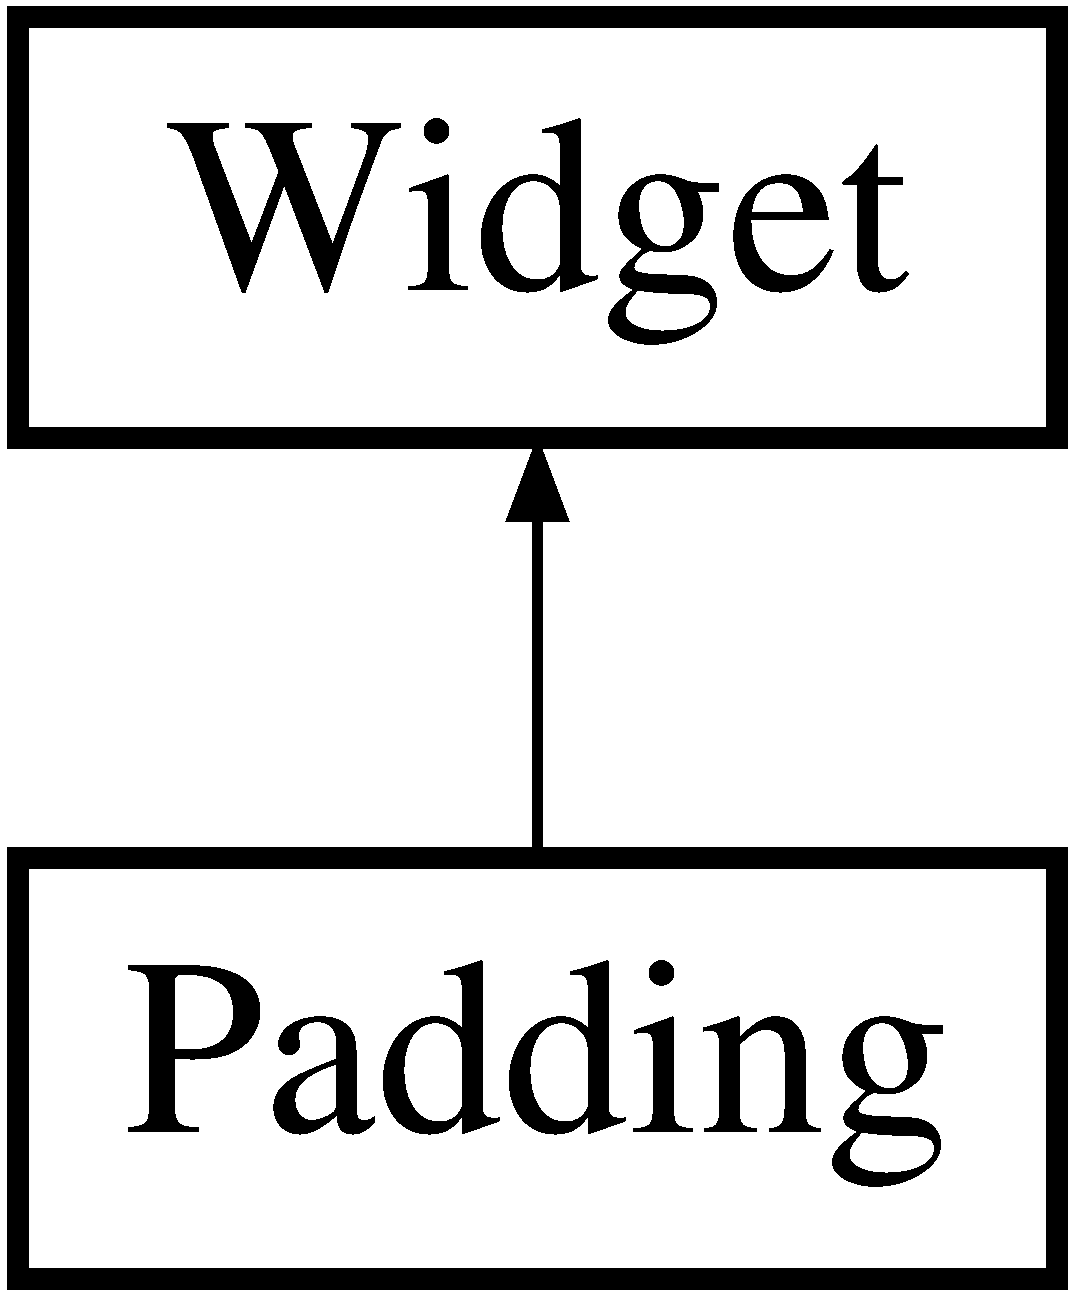
\includegraphics[height=2.000000cm]{classpadding_1_1_padding}
\end{center}
\end{figure}
\subsection*{Public Member Functions}
\begin{DoxyCompactItemize}
\item 
def \hyperlink{classpadding_1_1_padding_a9a6d706ad05cb94992492f5b9ef0c450}{\+\_\+\+\_\+init\+\_\+\+\_\+} (self, text=None)
\item 
def \hyperlink{classpadding_1_1_padding_acbcf633d6b24a3e818c168fe5ec6ef04}{do\+\_\+realize} (self)
\item 
def \hyperlink{classpadding_1_1_padding_a062833f2fdcd76c59e720632782ce086}{do\+\_\+unrealize} (self)
\item 
def \hyperlink{classpadding_1_1_padding_a3306e45c6b3b906dffe468ab31ddacf3}{do\+\_\+size\+\_\+request} (self, requisition)
\item 
def \hyperlink{classpadding_1_1_padding_aeecd5f975520316f3861bbdf3dc25b31}{do\+\_\+size\+\_\+allocate} (self, \hyperlink{classpadding_1_1_padding_a95abc93277d25eecef5c7599dfa4b330}{allocation})
\item 
def \hyperlink{classpadding_1_1_padding_a3568b624c8d5e9dd63c9073dfab5d1b4}{do\+\_\+expose\+\_\+event} (self, event)
\end{DoxyCompactItemize}
\subsection*{Data Fields}
\begin{DoxyCompactItemize}
\item 
\hyperlink{classpadding_1_1_padding_a04a8a2bbfa9c15500892b8e5033d625b}{window}
\item 
\hyperlink{classpadding_1_1_padding_a95abc93277d25eecef5c7599dfa4b330}{allocation}
\end{DoxyCompactItemize}


\subsection{Constructor \& Destructor Documentation}
\mbox{\Hypertarget{classpadding_1_1_padding_a9a6d706ad05cb94992492f5b9ef0c450}\label{classpadding_1_1_padding_a9a6d706ad05cb94992492f5b9ef0c450}} 
\index{padding\+::\+Padding@{padding\+::\+Padding}!\+\_\+\+\_\+init\+\_\+\+\_\+@{\+\_\+\+\_\+init\+\_\+\+\_\+}}
\index{\+\_\+\+\_\+init\+\_\+\+\_\+@{\+\_\+\+\_\+init\+\_\+\+\_\+}!padding\+::\+Padding@{padding\+::\+Padding}}
\subsubsection{\texorpdfstring{\+\_\+\+\_\+init\+\_\+\+\_\+()}{\_\_init\_\_()}}
{\footnotesize\ttfamily def \+\_\+\+\_\+init\+\_\+\+\_\+ (\begin{DoxyParamCaption}\item[{}]{self,  }\item[{}]{text = {\ttfamily None} }\end{DoxyParamCaption})}



\subsection{Member Function Documentation}
\mbox{\Hypertarget{classpadding_1_1_padding_a3568b624c8d5e9dd63c9073dfab5d1b4}\label{classpadding_1_1_padding_a3568b624c8d5e9dd63c9073dfab5d1b4}} 
\index{padding\+::\+Padding@{padding\+::\+Padding}!do\+\_\+expose\+\_\+event@{do\+\_\+expose\+\_\+event}}
\index{do\+\_\+expose\+\_\+event@{do\+\_\+expose\+\_\+event}!padding\+::\+Padding@{padding\+::\+Padding}}
\subsubsection{\texorpdfstring{do\+\_\+expose\+\_\+event()}{do\_expose\_event()}}
{\footnotesize\ttfamily def do\+\_\+expose\+\_\+event (\begin{DoxyParamCaption}\item[{}]{self,  }\item[{}]{event }\end{DoxyParamCaption})}

\mbox{\Hypertarget{classpadding_1_1_padding_acbcf633d6b24a3e818c168fe5ec6ef04}\label{classpadding_1_1_padding_acbcf633d6b24a3e818c168fe5ec6ef04}} 
\index{padding\+::\+Padding@{padding\+::\+Padding}!do\+\_\+realize@{do\+\_\+realize}}
\index{do\+\_\+realize@{do\+\_\+realize}!padding\+::\+Padding@{padding\+::\+Padding}}
\subsubsection{\texorpdfstring{do\+\_\+realize()}{do\_realize()}}
{\footnotesize\ttfamily def do\+\_\+realize (\begin{DoxyParamCaption}\item[{}]{self }\end{DoxyParamCaption})}

\mbox{\Hypertarget{classpadding_1_1_padding_aeecd5f975520316f3861bbdf3dc25b31}\label{classpadding_1_1_padding_aeecd5f975520316f3861bbdf3dc25b31}} 
\index{padding\+::\+Padding@{padding\+::\+Padding}!do\+\_\+size\+\_\+allocate@{do\+\_\+size\+\_\+allocate}}
\index{do\+\_\+size\+\_\+allocate@{do\+\_\+size\+\_\+allocate}!padding\+::\+Padding@{padding\+::\+Padding}}
\subsubsection{\texorpdfstring{do\+\_\+size\+\_\+allocate()}{do\_size\_allocate()}}
{\footnotesize\ttfamily def do\+\_\+size\+\_\+allocate (\begin{DoxyParamCaption}\item[{}]{self,  }\item[{}]{allocation }\end{DoxyParamCaption})}

\mbox{\Hypertarget{classpadding_1_1_padding_a3306e45c6b3b906dffe468ab31ddacf3}\label{classpadding_1_1_padding_a3306e45c6b3b906dffe468ab31ddacf3}} 
\index{padding\+::\+Padding@{padding\+::\+Padding}!do\+\_\+size\+\_\+request@{do\+\_\+size\+\_\+request}}
\index{do\+\_\+size\+\_\+request@{do\+\_\+size\+\_\+request}!padding\+::\+Padding@{padding\+::\+Padding}}
\subsubsection{\texorpdfstring{do\+\_\+size\+\_\+request()}{do\_size\_request()}}
{\footnotesize\ttfamily def do\+\_\+size\+\_\+request (\begin{DoxyParamCaption}\item[{}]{self,  }\item[{}]{requisition }\end{DoxyParamCaption})}

\mbox{\Hypertarget{classpadding_1_1_padding_a062833f2fdcd76c59e720632782ce086}\label{classpadding_1_1_padding_a062833f2fdcd76c59e720632782ce086}} 
\index{padding\+::\+Padding@{padding\+::\+Padding}!do\+\_\+unrealize@{do\+\_\+unrealize}}
\index{do\+\_\+unrealize@{do\+\_\+unrealize}!padding\+::\+Padding@{padding\+::\+Padding}}
\subsubsection{\texorpdfstring{do\+\_\+unrealize()}{do\_unrealize()}}
{\footnotesize\ttfamily def do\+\_\+unrealize (\begin{DoxyParamCaption}\item[{}]{self }\end{DoxyParamCaption})}



\subsection{Field Documentation}
\mbox{\Hypertarget{classpadding_1_1_padding_a95abc93277d25eecef5c7599dfa4b330}\label{classpadding_1_1_padding_a95abc93277d25eecef5c7599dfa4b330}} 
\index{padding\+::\+Padding@{padding\+::\+Padding}!allocation@{allocation}}
\index{allocation@{allocation}!padding\+::\+Padding@{padding\+::\+Padding}}
\subsubsection{\texorpdfstring{allocation}{allocation}}
{\footnotesize\ttfamily allocation}

\mbox{\Hypertarget{classpadding_1_1_padding_a04a8a2bbfa9c15500892b8e5033d625b}\label{classpadding_1_1_padding_a04a8a2bbfa9c15500892b8e5033d625b}} 
\index{padding\+::\+Padding@{padding\+::\+Padding}!window@{window}}
\index{window@{window}!padding\+::\+Padding@{padding\+::\+Padding}}
\subsubsection{\texorpdfstring{window}{window}}
{\footnotesize\ttfamily window}



The documentation for this class was generated from the following file\+:\begin{DoxyCompactItemize}
\item 
gui/\hyperlink{padding_8py}{padding.\+py}\end{DoxyCompactItemize}

\hypertarget{classyellow_1_1stick_doc}{}\section{stick\+Doc Class Reference}
\label{classyellow_1_1stick_doc}\index{stick\+Doc@{stick\+Doc}}
Inheritance diagram for stick\+Doc\+:\begin{figure}[H]
\begin{center}
\leavevmode
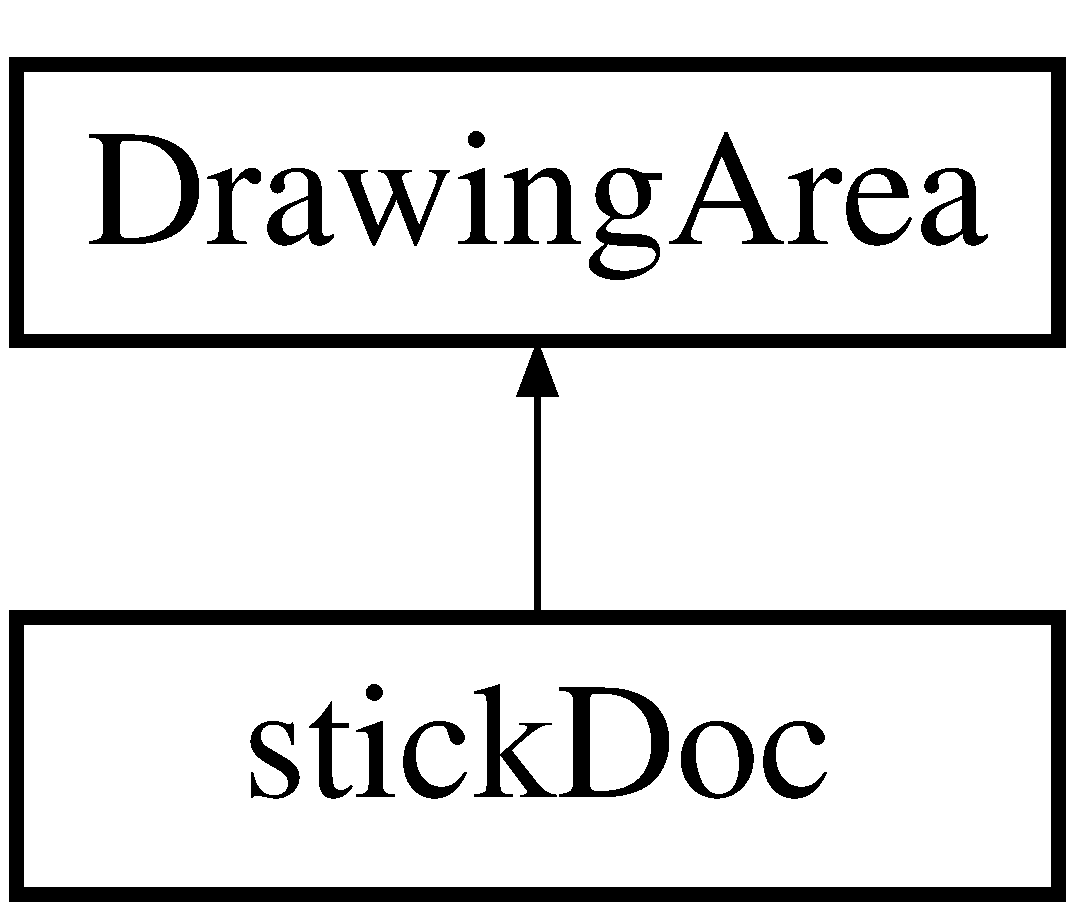
\includegraphics[height=2.000000cm]{classyellow_1_1stick_doc}
\end{center}
\end{figure}
\subsection*{Public Member Functions}
\begin{DoxyCompactItemize}
\item 
def \hyperlink{classyellow_1_1stick_doc_a6e4af27ccdc132f24f6e1cf523a4532b}{\+\_\+\+\_\+init\+\_\+\+\_\+} (self, \hyperlink{classyellow_1_1stick_doc_a8a4e5ec5926f293767f3c555868e4c21}{par}, \hyperlink{classyellow_1_1stick_doc_a434acd167ada209c34621739b6b8c583}{head}, \hyperlink{classyellow_1_1stick_doc_af575f17e6be3f269b86b041a60560dbf}{text})
\item 
def \hyperlink{classyellow_1_1stick_doc_a260d37924dae7e20867bbd197b9044ee}{area\+\_\+button} (self, area, event)
\item 
def \hyperlink{classyellow_1_1stick_doc_add4986c7f04102d45ce25c8e2510edf0}{area\+\_\+motion} (self, area, event)
\item 
def \hyperlink{classyellow_1_1stick_doc_aa33fa2b192b46f3d8e5e17d53a463f3c}{key\+\_\+press\+\_\+event} (self, text\+\_\+view, event)
\item 
def \hyperlink{classyellow_1_1stick_doc_a8f85a8233505e724112ad12098855c1d}{setfont} (self, fam, size)
\item 
def \hyperlink{classyellow_1_1stick_doc_a0730446d6038be2aa7f41b6a0262dfbe}{area\+\_\+expose\+\_\+cb} (self, area, event)
\end{DoxyCompactItemize}
\subsection*{Data Fields}
\begin{DoxyCompactItemize}
\item 
\hyperlink{classyellow_1_1stick_doc_a8a4e5ec5926f293767f3c555868e4c21}{par}
\item 
\hyperlink{classyellow_1_1stick_doc_af77a598ca5e5c4b3f9e19410edb7b5dc}{parwin}
\item 
\hyperlink{classyellow_1_1stick_doc_a434acd167ada209c34621739b6b8c583}{head}
\item 
\hyperlink{classyellow_1_1stick_doc_af575f17e6be3f269b86b041a60560dbf}{text}
\item 
\hyperlink{classyellow_1_1stick_doc_ac3572d35c0534d609c7df7c1b85f62bc}{gap}
\item 
\hyperlink{classyellow_1_1stick_doc_af6498084a79f833610813077daf71faa}{colormap}
\item 
\hyperlink{classyellow_1_1stick_doc_a350f90598ea332f936fea59cd1d149d7}{fgcolor}
\item 
\hyperlink{classyellow_1_1stick_doc_abc9ea27789a0328b83443cfe81b3e99f}{bgcolor}
\item 
\hyperlink{classyellow_1_1stick_doc_a7392854aec942bde0c9865f4b2fdbd5b}{frcolor}
\item 
\hyperlink{classyellow_1_1stick_doc_acadcfbe9531a84473f5c2dd3cefec767}{pangolayout}
\item 
\hyperlink{classyellow_1_1stick_doc_a7343e1995b4263df542facd235c7f129}{ex}
\item 
\hyperlink{classyellow_1_1stick_doc_a376b04dd893dc07de5fd20a21f7a08df}{ey}
\item 
\hyperlink{classyellow_1_1stick_doc_a3c777c2e882501a60f073f47e75ca153}{cyy}
\item 
\hyperlink{classyellow_1_1stick_doc_a4ba1825606cdadc883059651caa3ff4b}{gc}
\item 
\hyperlink{classyellow_1_1stick_doc_ae61e7de603852182385da5e907b4b232}{hh}
\end{DoxyCompactItemize}


\subsection{Constructor \& Destructor Documentation}
\mbox{\Hypertarget{classyellow_1_1stick_doc_a6e4af27ccdc132f24f6e1cf523a4532b}\label{classyellow_1_1stick_doc_a6e4af27ccdc132f24f6e1cf523a4532b}} 
\index{yellow\+::stick\+Doc@{yellow\+::stick\+Doc}!\+\_\+\+\_\+init\+\_\+\+\_\+@{\+\_\+\+\_\+init\+\_\+\+\_\+}}
\index{\+\_\+\+\_\+init\+\_\+\+\_\+@{\+\_\+\+\_\+init\+\_\+\+\_\+}!yellow\+::stick\+Doc@{yellow\+::stick\+Doc}}
\subsubsection{\texorpdfstring{\+\_\+\+\_\+init\+\_\+\+\_\+()}{\_\_init\_\_()}}
{\footnotesize\ttfamily def \+\_\+\+\_\+init\+\_\+\+\_\+ (\begin{DoxyParamCaption}\item[{}]{self,  }\item[{}]{par,  }\item[{}]{head,  }\item[{}]{text }\end{DoxyParamCaption})}



\subsection{Member Function Documentation}
\mbox{\Hypertarget{classyellow_1_1stick_doc_a260d37924dae7e20867bbd197b9044ee}\label{classyellow_1_1stick_doc_a260d37924dae7e20867bbd197b9044ee}} 
\index{yellow\+::stick\+Doc@{yellow\+::stick\+Doc}!area\+\_\+button@{area\+\_\+button}}
\index{area\+\_\+button@{area\+\_\+button}!yellow\+::stick\+Doc@{yellow\+::stick\+Doc}}
\subsubsection{\texorpdfstring{area\+\_\+button()}{area\_button()}}
{\footnotesize\ttfamily def area\+\_\+button (\begin{DoxyParamCaption}\item[{}]{self,  }\item[{}]{area,  }\item[{}]{event }\end{DoxyParamCaption})}

\mbox{\Hypertarget{classyellow_1_1stick_doc_a0730446d6038be2aa7f41b6a0262dfbe}\label{classyellow_1_1stick_doc_a0730446d6038be2aa7f41b6a0262dfbe}} 
\index{yellow\+::stick\+Doc@{yellow\+::stick\+Doc}!area\+\_\+expose\+\_\+cb@{area\+\_\+expose\+\_\+cb}}
\index{area\+\_\+expose\+\_\+cb@{area\+\_\+expose\+\_\+cb}!yellow\+::stick\+Doc@{yellow\+::stick\+Doc}}
\subsubsection{\texorpdfstring{area\+\_\+expose\+\_\+cb()}{area\_expose\_cb()}}
{\footnotesize\ttfamily def area\+\_\+expose\+\_\+cb (\begin{DoxyParamCaption}\item[{}]{self,  }\item[{}]{area,  }\item[{}]{event }\end{DoxyParamCaption})}

\mbox{\Hypertarget{classyellow_1_1stick_doc_add4986c7f04102d45ce25c8e2510edf0}\label{classyellow_1_1stick_doc_add4986c7f04102d45ce25c8e2510edf0}} 
\index{yellow\+::stick\+Doc@{yellow\+::stick\+Doc}!area\+\_\+motion@{area\+\_\+motion}}
\index{area\+\_\+motion@{area\+\_\+motion}!yellow\+::stick\+Doc@{yellow\+::stick\+Doc}}
\subsubsection{\texorpdfstring{area\+\_\+motion()}{area\_motion()}}
{\footnotesize\ttfamily def area\+\_\+motion (\begin{DoxyParamCaption}\item[{}]{self,  }\item[{}]{area,  }\item[{}]{event }\end{DoxyParamCaption})}

\mbox{\Hypertarget{classyellow_1_1stick_doc_aa33fa2b192b46f3d8e5e17d53a463f3c}\label{classyellow_1_1stick_doc_aa33fa2b192b46f3d8e5e17d53a463f3c}} 
\index{yellow\+::stick\+Doc@{yellow\+::stick\+Doc}!key\+\_\+press\+\_\+event@{key\+\_\+press\+\_\+event}}
\index{key\+\_\+press\+\_\+event@{key\+\_\+press\+\_\+event}!yellow\+::stick\+Doc@{yellow\+::stick\+Doc}}
\subsubsection{\texorpdfstring{key\+\_\+press\+\_\+event()}{key\_press\_event()}}
{\footnotesize\ttfamily def key\+\_\+press\+\_\+event (\begin{DoxyParamCaption}\item[{}]{self,  }\item[{}]{text\+\_\+view,  }\item[{}]{event }\end{DoxyParamCaption})}

\mbox{\Hypertarget{classyellow_1_1stick_doc_a8f85a8233505e724112ad12098855c1d}\label{classyellow_1_1stick_doc_a8f85a8233505e724112ad12098855c1d}} 
\index{yellow\+::stick\+Doc@{yellow\+::stick\+Doc}!setfont@{setfont}}
\index{setfont@{setfont}!yellow\+::stick\+Doc@{yellow\+::stick\+Doc}}
\subsubsection{\texorpdfstring{setfont()}{setfont()}}
{\footnotesize\ttfamily def setfont (\begin{DoxyParamCaption}\item[{}]{self,  }\item[{}]{fam,  }\item[{}]{size }\end{DoxyParamCaption})}



\subsection{Field Documentation}
\mbox{\Hypertarget{classyellow_1_1stick_doc_abc9ea27789a0328b83443cfe81b3e99f}\label{classyellow_1_1stick_doc_abc9ea27789a0328b83443cfe81b3e99f}} 
\index{yellow\+::stick\+Doc@{yellow\+::stick\+Doc}!bgcolor@{bgcolor}}
\index{bgcolor@{bgcolor}!yellow\+::stick\+Doc@{yellow\+::stick\+Doc}}
\subsubsection{\texorpdfstring{bgcolor}{bgcolor}}
{\footnotesize\ttfamily bgcolor}

\mbox{\Hypertarget{classyellow_1_1stick_doc_af6498084a79f833610813077daf71faa}\label{classyellow_1_1stick_doc_af6498084a79f833610813077daf71faa}} 
\index{yellow\+::stick\+Doc@{yellow\+::stick\+Doc}!colormap@{colormap}}
\index{colormap@{colormap}!yellow\+::stick\+Doc@{yellow\+::stick\+Doc}}
\subsubsection{\texorpdfstring{colormap}{colormap}}
{\footnotesize\ttfamily colormap}

\mbox{\Hypertarget{classyellow_1_1stick_doc_a3c777c2e882501a60f073f47e75ca153}\label{classyellow_1_1stick_doc_a3c777c2e882501a60f073f47e75ca153}} 
\index{yellow\+::stick\+Doc@{yellow\+::stick\+Doc}!cyy@{cyy}}
\index{cyy@{cyy}!yellow\+::stick\+Doc@{yellow\+::stick\+Doc}}
\subsubsection{\texorpdfstring{cyy}{cyy}}
{\footnotesize\ttfamily cyy}

\mbox{\Hypertarget{classyellow_1_1stick_doc_a7343e1995b4263df542facd235c7f129}\label{classyellow_1_1stick_doc_a7343e1995b4263df542facd235c7f129}} 
\index{yellow\+::stick\+Doc@{yellow\+::stick\+Doc}!ex@{ex}}
\index{ex@{ex}!yellow\+::stick\+Doc@{yellow\+::stick\+Doc}}
\subsubsection{\texorpdfstring{ex}{ex}}
{\footnotesize\ttfamily ex}

\mbox{\Hypertarget{classyellow_1_1stick_doc_a376b04dd893dc07de5fd20a21f7a08df}\label{classyellow_1_1stick_doc_a376b04dd893dc07de5fd20a21f7a08df}} 
\index{yellow\+::stick\+Doc@{yellow\+::stick\+Doc}!ey@{ey}}
\index{ey@{ey}!yellow\+::stick\+Doc@{yellow\+::stick\+Doc}}
\subsubsection{\texorpdfstring{ey}{ey}}
{\footnotesize\ttfamily ey}

\mbox{\Hypertarget{classyellow_1_1stick_doc_a350f90598ea332f936fea59cd1d149d7}\label{classyellow_1_1stick_doc_a350f90598ea332f936fea59cd1d149d7}} 
\index{yellow\+::stick\+Doc@{yellow\+::stick\+Doc}!fgcolor@{fgcolor}}
\index{fgcolor@{fgcolor}!yellow\+::stick\+Doc@{yellow\+::stick\+Doc}}
\subsubsection{\texorpdfstring{fgcolor}{fgcolor}}
{\footnotesize\ttfamily fgcolor}

\mbox{\Hypertarget{classyellow_1_1stick_doc_a7392854aec942bde0c9865f4b2fdbd5b}\label{classyellow_1_1stick_doc_a7392854aec942bde0c9865f4b2fdbd5b}} 
\index{yellow\+::stick\+Doc@{yellow\+::stick\+Doc}!frcolor@{frcolor}}
\index{frcolor@{frcolor}!yellow\+::stick\+Doc@{yellow\+::stick\+Doc}}
\subsubsection{\texorpdfstring{frcolor}{frcolor}}
{\footnotesize\ttfamily frcolor}

\mbox{\Hypertarget{classyellow_1_1stick_doc_ac3572d35c0534d609c7df7c1b85f62bc}\label{classyellow_1_1stick_doc_ac3572d35c0534d609c7df7c1b85f62bc}} 
\index{yellow\+::stick\+Doc@{yellow\+::stick\+Doc}!gap@{gap}}
\index{gap@{gap}!yellow\+::stick\+Doc@{yellow\+::stick\+Doc}}
\subsubsection{\texorpdfstring{gap}{gap}}
{\footnotesize\ttfamily gap}

\mbox{\Hypertarget{classyellow_1_1stick_doc_a4ba1825606cdadc883059651caa3ff4b}\label{classyellow_1_1stick_doc_a4ba1825606cdadc883059651caa3ff4b}} 
\index{yellow\+::stick\+Doc@{yellow\+::stick\+Doc}!gc@{gc}}
\index{gc@{gc}!yellow\+::stick\+Doc@{yellow\+::stick\+Doc}}
\subsubsection{\texorpdfstring{gc}{gc}}
{\footnotesize\ttfamily gc}

\mbox{\Hypertarget{classyellow_1_1stick_doc_a434acd167ada209c34621739b6b8c583}\label{classyellow_1_1stick_doc_a434acd167ada209c34621739b6b8c583}} 
\index{yellow\+::stick\+Doc@{yellow\+::stick\+Doc}!head@{head}}
\index{head@{head}!yellow\+::stick\+Doc@{yellow\+::stick\+Doc}}
\subsubsection{\texorpdfstring{head}{head}}
{\footnotesize\ttfamily head}

\mbox{\Hypertarget{classyellow_1_1stick_doc_ae61e7de603852182385da5e907b4b232}\label{classyellow_1_1stick_doc_ae61e7de603852182385da5e907b4b232}} 
\index{yellow\+::stick\+Doc@{yellow\+::stick\+Doc}!hh@{hh}}
\index{hh@{hh}!yellow\+::stick\+Doc@{yellow\+::stick\+Doc}}
\subsubsection{\texorpdfstring{hh}{hh}}
{\footnotesize\ttfamily hh}

\mbox{\Hypertarget{classyellow_1_1stick_doc_acadcfbe9531a84473f5c2dd3cefec767}\label{classyellow_1_1stick_doc_acadcfbe9531a84473f5c2dd3cefec767}} 
\index{yellow\+::stick\+Doc@{yellow\+::stick\+Doc}!pangolayout@{pangolayout}}
\index{pangolayout@{pangolayout}!yellow\+::stick\+Doc@{yellow\+::stick\+Doc}}
\subsubsection{\texorpdfstring{pangolayout}{pangolayout}}
{\footnotesize\ttfamily pangolayout}

\mbox{\Hypertarget{classyellow_1_1stick_doc_a8a4e5ec5926f293767f3c555868e4c21}\label{classyellow_1_1stick_doc_a8a4e5ec5926f293767f3c555868e4c21}} 
\index{yellow\+::stick\+Doc@{yellow\+::stick\+Doc}!par@{par}}
\index{par@{par}!yellow\+::stick\+Doc@{yellow\+::stick\+Doc}}
\subsubsection{\texorpdfstring{par}{par}}
{\footnotesize\ttfamily par}

\mbox{\Hypertarget{classyellow_1_1stick_doc_af77a598ca5e5c4b3f9e19410edb7b5dc}\label{classyellow_1_1stick_doc_af77a598ca5e5c4b3f9e19410edb7b5dc}} 
\index{yellow\+::stick\+Doc@{yellow\+::stick\+Doc}!parwin@{parwin}}
\index{parwin@{parwin}!yellow\+::stick\+Doc@{yellow\+::stick\+Doc}}
\subsubsection{\texorpdfstring{parwin}{parwin}}
{\footnotesize\ttfamily parwin}

\mbox{\Hypertarget{classyellow_1_1stick_doc_af575f17e6be3f269b86b041a60560dbf}\label{classyellow_1_1stick_doc_af575f17e6be3f269b86b041a60560dbf}} 
\index{yellow\+::stick\+Doc@{yellow\+::stick\+Doc}!text@{text}}
\index{text@{text}!yellow\+::stick\+Doc@{yellow\+::stick\+Doc}}
\subsubsection{\texorpdfstring{text}{text}}
{\footnotesize\ttfamily text}



The documentation for this class was generated from the following file\+:\begin{DoxyCompactItemize}
\item 
gui/\hyperlink{yellow_8py}{yellow.\+py}\end{DoxyCompactItemize}

\hypertarget{classyellow_1_1stick_list}{}\section{stick\+List Class Reference}
\label{classyellow_1_1stick_list}\index{stick\+List@{stick\+List}}
\subsection*{Public Member Functions}
\begin{DoxyCompactItemize}
\item 
def \hyperlink{classyellow_1_1stick_list_ae64f0875afe3067b97ba370b354b9213}{\+\_\+\+\_\+init\+\_\+\+\_\+} (self)
\item 
def \hyperlink{classyellow_1_1stick_list_a307b88adc33e3b4d944536007e3f841b}{add} (self, item)
\end{DoxyCompactItemize}
\subsection*{Data Fields}
\begin{DoxyCompactItemize}
\item 
\hyperlink{classyellow_1_1stick_list_a511ae0b1c13f95e5f08f1a0dd3da3d93}{data}
\end{DoxyCompactItemize}


\subsection{Constructor \& Destructor Documentation}
\mbox{\Hypertarget{classyellow_1_1stick_list_ae64f0875afe3067b97ba370b354b9213}\label{classyellow_1_1stick_list_ae64f0875afe3067b97ba370b354b9213}} 
\index{yellow\+::stick\+List@{yellow\+::stick\+List}!\+\_\+\+\_\+init\+\_\+\+\_\+@{\+\_\+\+\_\+init\+\_\+\+\_\+}}
\index{\+\_\+\+\_\+init\+\_\+\+\_\+@{\+\_\+\+\_\+init\+\_\+\+\_\+}!yellow\+::stick\+List@{yellow\+::stick\+List}}
\subsubsection{\texorpdfstring{\+\_\+\+\_\+init\+\_\+\+\_\+()}{\_\_init\_\_()}}
{\footnotesize\ttfamily def \+\_\+\+\_\+init\+\_\+\+\_\+ (\begin{DoxyParamCaption}\item[{}]{self }\end{DoxyParamCaption})}



\subsection{Member Function Documentation}
\mbox{\Hypertarget{classyellow_1_1stick_list_a307b88adc33e3b4d944536007e3f841b}\label{classyellow_1_1stick_list_a307b88adc33e3b4d944536007e3f841b}} 
\index{yellow\+::stick\+List@{yellow\+::stick\+List}!add@{add}}
\index{add@{add}!yellow\+::stick\+List@{yellow\+::stick\+List}}
\subsubsection{\texorpdfstring{add()}{add()}}
{\footnotesize\ttfamily def add (\begin{DoxyParamCaption}\item[{}]{self,  }\item[{}]{item }\end{DoxyParamCaption})}



\subsection{Field Documentation}
\mbox{\Hypertarget{classyellow_1_1stick_list_a511ae0b1c13f95e5f08f1a0dd3da3d93}\label{classyellow_1_1stick_list_a511ae0b1c13f95e5f08f1a0dd3da3d93}} 
\index{yellow\+::stick\+List@{yellow\+::stick\+List}!data@{data}}
\index{data@{data}!yellow\+::stick\+List@{yellow\+::stick\+List}}
\subsubsection{\texorpdfstring{data}{data}}
{\footnotesize\ttfamily data}



The documentation for this class was generated from the following file\+:\begin{DoxyCompactItemize}
\item 
gui/\hyperlink{yellow_8py}{yellow.\+py}\end{DoxyCompactItemize}

\hypertarget{classyellow_1_1stick_win}{}\section{stick\+Win Class Reference}
\label{classyellow_1_1stick_win}\index{stick\+Win@{stick\+Win}}
\subsection*{Public Member Functions}
\begin{DoxyCompactItemize}
\item 
def \hyperlink{classyellow_1_1stick_win_aa16d52e08a19e19e0a6aeb32c7702840}{\+\_\+\+\_\+init\+\_\+\+\_\+} (self, \hyperlink{classyellow_1_1stick_win_a9c2f924fb2f7004e7979ab2027ca1d65}{me}, \hyperlink{classyellow_1_1stick_win_a434acd167ada209c34621739b6b8c583}{head}, \hyperlink{classyellow_1_1stick_win_af575f17e6be3f269b86b041a60560dbf}{text})
\item 
def \hyperlink{classyellow_1_1stick_win_a260d37924dae7e20867bbd197b9044ee}{area\+\_\+button} (self, area, event)
\item 
def \hyperlink{classyellow_1_1stick_win_aa33fa2b192b46f3d8e5e17d53a463f3c}{key\+\_\+press\+\_\+event} (self, text\+\_\+view, event)
\item 
def \hyperlink{classyellow_1_1stick_win_a038ffcc265f4f83c2fbb952297dce8d7}{invalidate} (self, rect=None)
\item 
def \hyperlink{classyellow_1_1stick_win_a78b79da4bf62826f29316cd206c79241}{On\+Exit} (self, aa, bb=\char`\"{}\char`\"{})
\end{DoxyCompactItemize}
\subsection*{Data Fields}
\begin{DoxyCompactItemize}
\item 
\hyperlink{classyellow_1_1stick_win_a434acd167ada209c34621739b6b8c583}{head}
\item 
\hyperlink{classyellow_1_1stick_win_a9c2f924fb2f7004e7979ab2027ca1d65}{me}
\item 
\hyperlink{classyellow_1_1stick_win_af575f17e6be3f269b86b041a60560dbf}{text}
\item 
\hyperlink{classyellow_1_1stick_win_a04a8a2bbfa9c15500892b8e5033d625b}{window}
\item 
\hyperlink{classyellow_1_1stick_win_a56bf4260587baa1f272837175342b62a}{sticky}
\end{DoxyCompactItemize}


\subsection{Constructor \& Destructor Documentation}
\mbox{\Hypertarget{classyellow_1_1stick_win_aa16d52e08a19e19e0a6aeb32c7702840}\label{classyellow_1_1stick_win_aa16d52e08a19e19e0a6aeb32c7702840}} 
\index{yellow\+::stick\+Win@{yellow\+::stick\+Win}!\+\_\+\+\_\+init\+\_\+\+\_\+@{\+\_\+\+\_\+init\+\_\+\+\_\+}}
\index{\+\_\+\+\_\+init\+\_\+\+\_\+@{\+\_\+\+\_\+init\+\_\+\+\_\+}!yellow\+::stick\+Win@{yellow\+::stick\+Win}}
\subsubsection{\texorpdfstring{\+\_\+\+\_\+init\+\_\+\+\_\+()}{\_\_init\_\_()}}
{\footnotesize\ttfamily def \+\_\+\+\_\+init\+\_\+\+\_\+ (\begin{DoxyParamCaption}\item[{}]{self,  }\item[{}]{me,  }\item[{}]{head,  }\item[{}]{text }\end{DoxyParamCaption})}



\subsection{Member Function Documentation}
\mbox{\Hypertarget{classyellow_1_1stick_win_a260d37924dae7e20867bbd197b9044ee}\label{classyellow_1_1stick_win_a260d37924dae7e20867bbd197b9044ee}} 
\index{yellow\+::stick\+Win@{yellow\+::stick\+Win}!area\+\_\+button@{area\+\_\+button}}
\index{area\+\_\+button@{area\+\_\+button}!yellow\+::stick\+Win@{yellow\+::stick\+Win}}
\subsubsection{\texorpdfstring{area\+\_\+button()}{area\_button()}}
{\footnotesize\ttfamily def area\+\_\+button (\begin{DoxyParamCaption}\item[{}]{self,  }\item[{}]{area,  }\item[{}]{event }\end{DoxyParamCaption})}

\mbox{\Hypertarget{classyellow_1_1stick_win_a038ffcc265f4f83c2fbb952297dce8d7}\label{classyellow_1_1stick_win_a038ffcc265f4f83c2fbb952297dce8d7}} 
\index{yellow\+::stick\+Win@{yellow\+::stick\+Win}!invalidate@{invalidate}}
\index{invalidate@{invalidate}!yellow\+::stick\+Win@{yellow\+::stick\+Win}}
\subsubsection{\texorpdfstring{invalidate()}{invalidate()}}
{\footnotesize\ttfamily def invalidate (\begin{DoxyParamCaption}\item[{}]{self,  }\item[{}]{rect = {\ttfamily None} }\end{DoxyParamCaption})}

\mbox{\Hypertarget{classyellow_1_1stick_win_aa33fa2b192b46f3d8e5e17d53a463f3c}\label{classyellow_1_1stick_win_aa33fa2b192b46f3d8e5e17d53a463f3c}} 
\index{yellow\+::stick\+Win@{yellow\+::stick\+Win}!key\+\_\+press\+\_\+event@{key\+\_\+press\+\_\+event}}
\index{key\+\_\+press\+\_\+event@{key\+\_\+press\+\_\+event}!yellow\+::stick\+Win@{yellow\+::stick\+Win}}
\subsubsection{\texorpdfstring{key\+\_\+press\+\_\+event()}{key\_press\_event()}}
{\footnotesize\ttfamily def key\+\_\+press\+\_\+event (\begin{DoxyParamCaption}\item[{}]{self,  }\item[{}]{text\+\_\+view,  }\item[{}]{event }\end{DoxyParamCaption})}

\mbox{\Hypertarget{classyellow_1_1stick_win_a78b79da4bf62826f29316cd206c79241}\label{classyellow_1_1stick_win_a78b79da4bf62826f29316cd206c79241}} 
\index{yellow\+::stick\+Win@{yellow\+::stick\+Win}!On\+Exit@{On\+Exit}}
\index{On\+Exit@{On\+Exit}!yellow\+::stick\+Win@{yellow\+::stick\+Win}}
\subsubsection{\texorpdfstring{On\+Exit()}{OnExit()}}
{\footnotesize\ttfamily def On\+Exit (\begin{DoxyParamCaption}\item[{}]{self,  }\item[{}]{aa,  }\item[{}]{bb = {\ttfamily \char`\"{}\char`\"{}} }\end{DoxyParamCaption})}



\subsection{Field Documentation}
\mbox{\Hypertarget{classyellow_1_1stick_win_a434acd167ada209c34621739b6b8c583}\label{classyellow_1_1stick_win_a434acd167ada209c34621739b6b8c583}} 
\index{yellow\+::stick\+Win@{yellow\+::stick\+Win}!head@{head}}
\index{head@{head}!yellow\+::stick\+Win@{yellow\+::stick\+Win}}
\subsubsection{\texorpdfstring{head}{head}}
{\footnotesize\ttfamily head}

\mbox{\Hypertarget{classyellow_1_1stick_win_a9c2f924fb2f7004e7979ab2027ca1d65}\label{classyellow_1_1stick_win_a9c2f924fb2f7004e7979ab2027ca1d65}} 
\index{yellow\+::stick\+Win@{yellow\+::stick\+Win}!me@{me}}
\index{me@{me}!yellow\+::stick\+Win@{yellow\+::stick\+Win}}
\subsubsection{\texorpdfstring{me}{me}}
{\footnotesize\ttfamily me}

\mbox{\Hypertarget{classyellow_1_1stick_win_a56bf4260587baa1f272837175342b62a}\label{classyellow_1_1stick_win_a56bf4260587baa1f272837175342b62a}} 
\index{yellow\+::stick\+Win@{yellow\+::stick\+Win}!sticky@{sticky}}
\index{sticky@{sticky}!yellow\+::stick\+Win@{yellow\+::stick\+Win}}
\subsubsection{\texorpdfstring{sticky}{sticky}}
{\footnotesize\ttfamily sticky}

\mbox{\Hypertarget{classyellow_1_1stick_win_af575f17e6be3f269b86b041a60560dbf}\label{classyellow_1_1stick_win_af575f17e6be3f269b86b041a60560dbf}} 
\index{yellow\+::stick\+Win@{yellow\+::stick\+Win}!text@{text}}
\index{text@{text}!yellow\+::stick\+Win@{yellow\+::stick\+Win}}
\subsubsection{\texorpdfstring{text}{text}}
{\footnotesize\ttfamily text}

\mbox{\Hypertarget{classyellow_1_1stick_win_a04a8a2bbfa9c15500892b8e5033d625b}\label{classyellow_1_1stick_win_a04a8a2bbfa9c15500892b8e5033d625b}} 
\index{yellow\+::stick\+Win@{yellow\+::stick\+Win}!window@{window}}
\index{window@{window}!yellow\+::stick\+Win@{yellow\+::stick\+Win}}
\subsubsection{\texorpdfstring{window}{window}}
{\footnotesize\ttfamily window}



The documentation for this class was generated from the following file\+:\begin{DoxyCompactItemize}
\item 
gui/\hyperlink{yellow_8py}{yellow.\+py}\end{DoxyCompactItemize}

\hypertarget{classtreehand_1_1_tree_hand}{}\section{Tree\+Hand Class Reference}
\label{classtreehand_1_1_tree_hand}\index{Tree\+Hand@{Tree\+Hand}}
\subsection*{Public Member Functions}
\begin{DoxyCompactItemize}
\item 
def \hyperlink{classtreehand_1_1_tree_hand_aabaa7e33eed1ddc64a302cedbc99b421}{\+\_\+\+\_\+init\+\_\+\+\_\+} (self, tree\+\_\+sel\+\_\+row)
\item 
def \hyperlink{classtreehand_1_1_tree_hand_a0b8b6c3225e291dcb9b9ce13d6292b2a}{start\+\_\+tree} (self)
\item 
def \hyperlink{classtreehand_1_1_tree_hand_a916011b9ffb69624d31665f8cd2c494d}{create\+\_\+tree} (self, match, text=None)
\item 
def \hyperlink{classtreehand_1_1_tree_hand_a7fc3506055afa66f0a11d5e5445b8729}{update\+\_\+treestore} (self, text)
\item 
def \hyperlink{classtreehand_1_1_tree_hand_a54f38a035dfb7d513590e21e097aafc6}{append\+\_\+treestore} (self, text)
\end{DoxyCompactItemize}
\subsection*{Data Fields}
\begin{DoxyCompactItemize}
\item 
\hyperlink{classtreehand_1_1_tree_hand_a555b9539fb020fe8fb52e7c61eceda72}{treestore}
\item 
\hyperlink{classtreehand_1_1_tree_hand_a76dbcfc78e812394f40977b0e13a3a47}{tree}
\item 
\hyperlink{classtreehand_1_1_tree_hand_ac25c0ac677bf2b00e27bd937730b0964}{stree}
\end{DoxyCompactItemize}


\subsection{Constructor \& Destructor Documentation}
\mbox{\Hypertarget{classtreehand_1_1_tree_hand_aabaa7e33eed1ddc64a302cedbc99b421}\label{classtreehand_1_1_tree_hand_aabaa7e33eed1ddc64a302cedbc99b421}} 
\index{treehand\+::\+Tree\+Hand@{treehand\+::\+Tree\+Hand}!\+\_\+\+\_\+init\+\_\+\+\_\+@{\+\_\+\+\_\+init\+\_\+\+\_\+}}
\index{\+\_\+\+\_\+init\+\_\+\+\_\+@{\+\_\+\+\_\+init\+\_\+\+\_\+}!treehand\+::\+Tree\+Hand@{treehand\+::\+Tree\+Hand}}
\subsubsection{\texorpdfstring{\+\_\+\+\_\+init\+\_\+\+\_\+()}{\_\_init\_\_()}}
{\footnotesize\ttfamily def \+\_\+\+\_\+init\+\_\+\+\_\+ (\begin{DoxyParamCaption}\item[{}]{self,  }\item[{}]{tree\+\_\+sel\+\_\+row }\end{DoxyParamCaption})}



\subsection{Member Function Documentation}
\mbox{\Hypertarget{classtreehand_1_1_tree_hand_a54f38a035dfb7d513590e21e097aafc6}\label{classtreehand_1_1_tree_hand_a54f38a035dfb7d513590e21e097aafc6}} 
\index{treehand\+::\+Tree\+Hand@{treehand\+::\+Tree\+Hand}!append\+\_\+treestore@{append\+\_\+treestore}}
\index{append\+\_\+treestore@{append\+\_\+treestore}!treehand\+::\+Tree\+Hand@{treehand\+::\+Tree\+Hand}}
\subsubsection{\texorpdfstring{append\+\_\+treestore()}{append\_treestore()}}
{\footnotesize\ttfamily def append\+\_\+treestore (\begin{DoxyParamCaption}\item[{}]{self,  }\item[{}]{text }\end{DoxyParamCaption})}

\mbox{\Hypertarget{classtreehand_1_1_tree_hand_a916011b9ffb69624d31665f8cd2c494d}\label{classtreehand_1_1_tree_hand_a916011b9ffb69624d31665f8cd2c494d}} 
\index{treehand\+::\+Tree\+Hand@{treehand\+::\+Tree\+Hand}!create\+\_\+tree@{create\+\_\+tree}}
\index{create\+\_\+tree@{create\+\_\+tree}!treehand\+::\+Tree\+Hand@{treehand\+::\+Tree\+Hand}}
\subsubsection{\texorpdfstring{create\+\_\+tree()}{create\_tree()}}
{\footnotesize\ttfamily def create\+\_\+tree (\begin{DoxyParamCaption}\item[{}]{self,  }\item[{}]{match,  }\item[{}]{text = {\ttfamily None} }\end{DoxyParamCaption})}

\mbox{\Hypertarget{classtreehand_1_1_tree_hand_a0b8b6c3225e291dcb9b9ce13d6292b2a}\label{classtreehand_1_1_tree_hand_a0b8b6c3225e291dcb9b9ce13d6292b2a}} 
\index{treehand\+::\+Tree\+Hand@{treehand\+::\+Tree\+Hand}!start\+\_\+tree@{start\+\_\+tree}}
\index{start\+\_\+tree@{start\+\_\+tree}!treehand\+::\+Tree\+Hand@{treehand\+::\+Tree\+Hand}}
\subsubsection{\texorpdfstring{start\+\_\+tree()}{start\_tree()}}
{\footnotesize\ttfamily def start\+\_\+tree (\begin{DoxyParamCaption}\item[{}]{self }\end{DoxyParamCaption})}

\mbox{\Hypertarget{classtreehand_1_1_tree_hand_a7fc3506055afa66f0a11d5e5445b8729}\label{classtreehand_1_1_tree_hand_a7fc3506055afa66f0a11d5e5445b8729}} 
\index{treehand\+::\+Tree\+Hand@{treehand\+::\+Tree\+Hand}!update\+\_\+treestore@{update\+\_\+treestore}}
\index{update\+\_\+treestore@{update\+\_\+treestore}!treehand\+::\+Tree\+Hand@{treehand\+::\+Tree\+Hand}}
\subsubsection{\texorpdfstring{update\+\_\+treestore()}{update\_treestore()}}
{\footnotesize\ttfamily def update\+\_\+treestore (\begin{DoxyParamCaption}\item[{}]{self,  }\item[{}]{text }\end{DoxyParamCaption})}



\subsection{Field Documentation}
\mbox{\Hypertarget{classtreehand_1_1_tree_hand_ac25c0ac677bf2b00e27bd937730b0964}\label{classtreehand_1_1_tree_hand_ac25c0ac677bf2b00e27bd937730b0964}} 
\index{treehand\+::\+Tree\+Hand@{treehand\+::\+Tree\+Hand}!stree@{stree}}
\index{stree@{stree}!treehand\+::\+Tree\+Hand@{treehand\+::\+Tree\+Hand}}
\subsubsection{\texorpdfstring{stree}{stree}}
{\footnotesize\ttfamily stree}

\mbox{\Hypertarget{classtreehand_1_1_tree_hand_a76dbcfc78e812394f40977b0e13a3a47}\label{classtreehand_1_1_tree_hand_a76dbcfc78e812394f40977b0e13a3a47}} 
\index{treehand\+::\+Tree\+Hand@{treehand\+::\+Tree\+Hand}!tree@{tree}}
\index{tree@{tree}!treehand\+::\+Tree\+Hand@{treehand\+::\+Tree\+Hand}}
\subsubsection{\texorpdfstring{tree}{tree}}
{\footnotesize\ttfamily tree}

\mbox{\Hypertarget{classtreehand_1_1_tree_hand_a555b9539fb020fe8fb52e7c61eceda72}\label{classtreehand_1_1_tree_hand_a555b9539fb020fe8fb52e7c61eceda72}} 
\index{treehand\+::\+Tree\+Hand@{treehand\+::\+Tree\+Hand}!treestore@{treestore}}
\index{treestore@{treestore}!treehand\+::\+Tree\+Hand@{treehand\+::\+Tree\+Hand}}
\subsubsection{\texorpdfstring{treestore}{treestore}}
{\footnotesize\ttfamily treestore}



The documentation for this class was generated from the following file\+:\begin{DoxyCompactItemize}
\item 
gui/\hyperlink{treehand_8py}{treehand.\+py}\end{DoxyCompactItemize}

\chapter{File Documentation}
\hypertarget{block__blue2_8c}{}\section{bluepoint/block\+\_\+blue2.c File Reference}
\label{block__blue2_8c}\index{bluepoint/block\+\_\+blue2.\+c@{bluepoint/block\+\_\+blue2.\+c}}
{\ttfamily \#include \char`\"{}stdlib.\+h\char`\"{}}\newline
{\ttfamily \#include \char`\"{}stdio.\+h\char`\"{}}\newline
{\ttfamily \#include \char`\"{}string.\+h\char`\"{}}\newline
{\ttfamily \#include \char`\"{}bluepoint2.\+h\char`\"{}}\newline
{\ttfamily \#include \char`\"{}hs\+\_\+crypt.\+c\char`\"{}}\newline
\subsection*{Data Structures}
\begin{DoxyCompactItemize}
\item 
struct \hyperlink{structcentinel}{centinel}
\end{DoxyCompactItemize}
\subsection*{Macros}
\begin{DoxyCompactItemize}
\item 
\#define \hyperlink{block__blue2_8c_abfae0751b37c27838de316a9e644021d}{D\+E\+F\+\_\+\+D\+U\+M\+P\+H\+EX}~1
\item 
\#define \hyperlink{block__blue2_8c_afcf795f5a96fd55561abe69f56224630}{B\+L\+O\+C\+K\+S\+I\+ZE}~1024
\end{DoxyCompactItemize}
\subsection*{Functions}
\begin{DoxyCompactItemize}
\item 
int \hyperlink{block__blue2_8c_af526355f72b6cec33051ff28a7971088}{sdump} (void $\ast$mem)
\item 
int \hyperlink{block__blue2_8c_a0ddf1224851353fc92bfbff6f499fa97}{main} (int argc, char $\ast$argv\mbox{[}$\,$\mbox{]})
\end{DoxyCompactItemize}
\subsection*{Variables}
\begin{DoxyCompactItemize}
\item 
struct \hyperlink{structcentinel}{centinel} \hyperlink{block__blue2_8c_a35fb1b7a8669f9c10da4d2947fbde2d1}{cent}
\item 
char \hyperlink{block__blue2_8c_a010542bf29e182284896c9c2f42e1387}{pass} \mbox{[}128\mbox{]} = \char`\"{}1234\char`\"{}
\item 
int \hyperlink{block__blue2_8c_a77e5778dba48d5d75c364f1c6f9f5da4}{slen}
\item 
int \hyperlink{block__blue2_8c_ad29d2259942853507dff3a3e3c05535a}{plen}
\end{DoxyCompactItemize}


\subsection{Macro Definition Documentation}
\mbox{\Hypertarget{block__blue2_8c_afcf795f5a96fd55561abe69f56224630}\label{block__blue2_8c_afcf795f5a96fd55561abe69f56224630}} 
\index{block\+\_\+blue2.\+c@{block\+\_\+blue2.\+c}!B\+L\+O\+C\+K\+S\+I\+ZE@{B\+L\+O\+C\+K\+S\+I\+ZE}}
\index{B\+L\+O\+C\+K\+S\+I\+ZE@{B\+L\+O\+C\+K\+S\+I\+ZE}!block\+\_\+blue2.\+c@{block\+\_\+blue2.\+c}}
\subsubsection{\texorpdfstring{B\+L\+O\+C\+K\+S\+I\+ZE}{BLOCKSIZE}}
{\footnotesize\ttfamily \#define B\+L\+O\+C\+K\+S\+I\+ZE~1024}

\mbox{\Hypertarget{block__blue2_8c_abfae0751b37c27838de316a9e644021d}\label{block__blue2_8c_abfae0751b37c27838de316a9e644021d}} 
\index{block\+\_\+blue2.\+c@{block\+\_\+blue2.\+c}!D\+E\+F\+\_\+\+D\+U\+M\+P\+H\+EX@{D\+E\+F\+\_\+\+D\+U\+M\+P\+H\+EX}}
\index{D\+E\+F\+\_\+\+D\+U\+M\+P\+H\+EX@{D\+E\+F\+\_\+\+D\+U\+M\+P\+H\+EX}!block\+\_\+blue2.\+c@{block\+\_\+blue2.\+c}}
\subsubsection{\texorpdfstring{D\+E\+F\+\_\+\+D\+U\+M\+P\+H\+EX}{DEF\_DUMPHEX}}
{\footnotesize\ttfamily \#define D\+E\+F\+\_\+\+D\+U\+M\+P\+H\+EX~1}



\subsection{Function Documentation}
\mbox{\Hypertarget{block__blue2_8c_a0ddf1224851353fc92bfbff6f499fa97}\label{block__blue2_8c_a0ddf1224851353fc92bfbff6f499fa97}} 
\index{block\+\_\+blue2.\+c@{block\+\_\+blue2.\+c}!main@{main}}
\index{main@{main}!block\+\_\+blue2.\+c@{block\+\_\+blue2.\+c}}
\subsubsection{\texorpdfstring{main()}{main()}}
{\footnotesize\ttfamily int main (\begin{DoxyParamCaption}\item[{int}]{argc,  }\item[{char $\ast$}]{argv\mbox{[}$\,$\mbox{]} }\end{DoxyParamCaption})}

\mbox{\Hypertarget{block__blue2_8c_af526355f72b6cec33051ff28a7971088}\label{block__blue2_8c_af526355f72b6cec33051ff28a7971088}} 
\index{block\+\_\+blue2.\+c@{block\+\_\+blue2.\+c}!sdump@{sdump}}
\index{sdump@{sdump}!block\+\_\+blue2.\+c@{block\+\_\+blue2.\+c}}
\subsubsection{\texorpdfstring{sdump()}{sdump()}}
{\footnotesize\ttfamily int sdump (\begin{DoxyParamCaption}\item[{void $\ast$}]{mem }\end{DoxyParamCaption})}



\subsection{Variable Documentation}
\mbox{\Hypertarget{block__blue2_8c_a35fb1b7a8669f9c10da4d2947fbde2d1}\label{block__blue2_8c_a35fb1b7a8669f9c10da4d2947fbde2d1}} 
\index{block\+\_\+blue2.\+c@{block\+\_\+blue2.\+c}!cent@{cent}}
\index{cent@{cent}!block\+\_\+blue2.\+c@{block\+\_\+blue2.\+c}}
\subsubsection{\texorpdfstring{cent}{cent}}
{\footnotesize\ttfamily struct \hyperlink{structcentinel}{centinel}  cent}

\mbox{\Hypertarget{block__blue2_8c_a010542bf29e182284896c9c2f42e1387}\label{block__blue2_8c_a010542bf29e182284896c9c2f42e1387}} 
\index{block\+\_\+blue2.\+c@{block\+\_\+blue2.\+c}!pass@{pass}}
\index{pass@{pass}!block\+\_\+blue2.\+c@{block\+\_\+blue2.\+c}}
\subsubsection{\texorpdfstring{pass}{pass}}
{\footnotesize\ttfamily char pass\mbox{[}128\mbox{]} = \char`\"{}1234\char`\"{}}

\mbox{\Hypertarget{block__blue2_8c_ad29d2259942853507dff3a3e3c05535a}\label{block__blue2_8c_ad29d2259942853507dff3a3e3c05535a}} 
\index{block\+\_\+blue2.\+c@{block\+\_\+blue2.\+c}!plen@{plen}}
\index{plen@{plen}!block\+\_\+blue2.\+c@{block\+\_\+blue2.\+c}}
\subsubsection{\texorpdfstring{plen}{plen}}
{\footnotesize\ttfamily int plen}

\mbox{\Hypertarget{block__blue2_8c_a77e5778dba48d5d75c364f1c6f9f5da4}\label{block__blue2_8c_a77e5778dba48d5d75c364f1c6f9f5da4}} 
\index{block\+\_\+blue2.\+c@{block\+\_\+blue2.\+c}!slen@{slen}}
\index{slen@{slen}!block\+\_\+blue2.\+c@{block\+\_\+blue2.\+c}}
\subsubsection{\texorpdfstring{slen}{slen}}
{\footnotesize\ttfamily int slen}


\hypertarget{bluedecrypt_8c}{}\section{bluepoint/bluedecrypt.c File Reference}
\label{bluedecrypt_8c}\index{bluepoint/bluedecrypt.\+c@{bluepoint/bluedecrypt.\+c}}
{\ttfamily \#include $<$unistd.\+h$>$}\newline
{\ttfamily \#include $<$stdio.\+h$>$}\newline
{\ttfamily \#include $<$stddef.\+h$>$}\newline
{\ttfamily \#include $<$stdlib.\+h$>$}\newline
{\ttfamily \#include $<$stdarg.\+h$>$}\newline
{\ttfamily \#include $<$time.\+h$>$}\newline
{\ttfamily \#include $<$string.\+h$>$}\newline
{\ttfamily \#include $<$signal.\+h$>$}\newline
{\ttfamily \#include \char`\"{}getpass.\+h\char`\"{}}\newline
{\ttfamily \#include \char`\"{}base64.\+h\char`\"{}}\newline
{\ttfamily \#include \char`\"{}zmalloc.\+h\char`\"{}}\newline
{\ttfamily \#include \char`\"{}cmdline.\+h\char`\"{}}\newline
{\ttfamily \#include \char`\"{}bluepoint3.\+h\char`\"{}}\newline
{\ttfamily \#include \char`\"{}misc.\+h\char`\"{}}\newline
\subsection*{Functions}
\begin{DoxyCompactItemize}
\item 
void \hyperlink{bluedecrypt_8c_a4dfa2bd7b47512180fb611fddea9b3af}{xerr2} (const char $\ast$msg,...)
\item 
char $\ast$ \hyperlink{bluedecrypt_8c_a3352da1728927ec5d3f40b90eab4176f}{bluepoint\+\_\+hash\+\_\+file} (char $\ast$fname, char $\ast$$\ast$err\+\_\+str)
\item 
int \hyperlink{bluedecrypt_8c_a3c04138a5bfe5d72780bb7e82a18e627}{main} (int argc, char $\ast$$\ast$argv)
\end{DoxyCompactItemize}
\subsection*{Variables}
\begin{DoxyCompactItemize}
\item 
\hyperlink{cmdline_8h_a5ba458a06f0f7fe23f0cc0ce4003ad62}{opts} \hyperlink{bluedecrypt_8c_ad75e49d295005b3f5fffec85f24090d3}{opts\+\_\+data} \mbox{[}$\,$\mbox{]}
\end{DoxyCompactItemize}


\subsection{Function Documentation}
\mbox{\Hypertarget{bluedecrypt_8c_a3352da1728927ec5d3f40b90eab4176f}\label{bluedecrypt_8c_a3352da1728927ec5d3f40b90eab4176f}} 
\index{bluedecrypt.\+c@{bluedecrypt.\+c}!bluepoint\+\_\+hash\+\_\+file@{bluepoint\+\_\+hash\+\_\+file}}
\index{bluepoint\+\_\+hash\+\_\+file@{bluepoint\+\_\+hash\+\_\+file}!bluedecrypt.\+c@{bluedecrypt.\+c}}
\subsubsection{\texorpdfstring{bluepoint\+\_\+hash\+\_\+file()}{bluepoint\_hash\_file()}}
{\footnotesize\ttfamily char$\ast$ bluepoint\+\_\+hash\+\_\+file (\begin{DoxyParamCaption}\item[{char $\ast$}]{fname,  }\item[{char $\ast$$\ast$}]{err\+\_\+str }\end{DoxyParamCaption})}

\mbox{\Hypertarget{bluedecrypt_8c_a3c04138a5bfe5d72780bb7e82a18e627}\label{bluedecrypt_8c_a3c04138a5bfe5d72780bb7e82a18e627}} 
\index{bluedecrypt.\+c@{bluedecrypt.\+c}!main@{main}}
\index{main@{main}!bluedecrypt.\+c@{bluedecrypt.\+c}}
\subsubsection{\texorpdfstring{main()}{main()}}
{\footnotesize\ttfamily int main (\begin{DoxyParamCaption}\item[{int}]{argc,  }\item[{char $\ast$$\ast$}]{argv }\end{DoxyParamCaption})}

\mbox{\Hypertarget{bluedecrypt_8c_a4dfa2bd7b47512180fb611fddea9b3af}\label{bluedecrypt_8c_a4dfa2bd7b47512180fb611fddea9b3af}} 
\index{bluedecrypt.\+c@{bluedecrypt.\+c}!xerr2@{xerr2}}
\index{xerr2@{xerr2}!bluedecrypt.\+c@{bluedecrypt.\+c}}
\subsubsection{\texorpdfstring{xerr2()}{xerr2()}}
{\footnotesize\ttfamily void xerr2 (\begin{DoxyParamCaption}\item[{const char $\ast$}]{msg,  }\item[{}]{... }\end{DoxyParamCaption})}



\subsection{Variable Documentation}
\mbox{\Hypertarget{bluedecrypt_8c_ad75e49d295005b3f5fffec85f24090d3}\label{bluedecrypt_8c_ad75e49d295005b3f5fffec85f24090d3}} 
\index{bluedecrypt.\+c@{bluedecrypt.\+c}!opts\+\_\+data@{opts\+\_\+data}}
\index{opts\+\_\+data@{opts\+\_\+data}!bluedecrypt.\+c@{bluedecrypt.\+c}}
\subsubsection{\texorpdfstring{opts\+\_\+data}{opts\_data}}
{\footnotesize\ttfamily \hyperlink{cmdline_8h_a5ba458a06f0f7fe23f0cc0ce4003ad62}{opts} opts\+\_\+data\mbox{[}$\,$\mbox{]}}


\hypertarget{blueencrypt_8c}{}\section{bluepoint/blueencrypt.c File Reference}
\label{blueencrypt_8c}\index{bluepoint/blueencrypt.\+c@{bluepoint/blueencrypt.\+c}}
{\ttfamily \#include $<$unistd.\+h$>$}\newline
{\ttfamily \#include $<$stdio.\+h$>$}\newline
{\ttfamily \#include $<$stddef.\+h$>$}\newline
{\ttfamily \#include $<$stdlib.\+h$>$}\newline
{\ttfamily \#include $<$stdarg.\+h$>$}\newline
{\ttfamily \#include $<$time.\+h$>$}\newline
{\ttfamily \#include $<$string.\+h$>$}\newline
{\ttfamily \#include $<$signal.\+h$>$}\newline
{\ttfamily \#include \char`\"{}getpass.\+h\char`\"{}}\newline
{\ttfamily \#include \char`\"{}base64.\+h\char`\"{}}\newline
{\ttfamily \#include \char`\"{}zmalloc.\+h\char`\"{}}\newline
{\ttfamily \#include \char`\"{}cmdline.\+h\char`\"{}}\newline
{\ttfamily \#include \char`\"{}bluepoint3.\+h\char`\"{}}\newline
{\ttfamily \#include \char`\"{}blueutil.\+h\char`\"{}}\newline
{\ttfamily \#include \char`\"{}misc.\+h\char`\"{}}\newline
\subsection*{Functions}
\begin{DoxyCompactItemize}
\item 
void \hyperlink{blueencrypt_8c_a4dfa2bd7b47512180fb611fddea9b3af}{xerr2} (const char $\ast$msg,...)
\item 
char $\ast$ \hyperlink{blueencrypt_8c_a3352da1728927ec5d3f40b90eab4176f}{bluepoint\+\_\+hash\+\_\+file} (char $\ast$fname, char $\ast$$\ast$err\+\_\+str)
\item 
int \hyperlink{blueencrypt_8c_a3c04138a5bfe5d72780bb7e82a18e627}{main} (int argc, char $\ast$$\ast$argv)
\end{DoxyCompactItemize}
\subsection*{Variables}
\begin{DoxyCompactItemize}
\item 
\hyperlink{cmdline_8h_a5ba458a06f0f7fe23f0cc0ce4003ad62}{opts} \hyperlink{blueencrypt_8c_ad75e49d295005b3f5fffec85f24090d3}{opts\+\_\+data} \mbox{[}$\,$\mbox{]}
\end{DoxyCompactItemize}


\subsection{Function Documentation}
\mbox{\Hypertarget{blueencrypt_8c_a3352da1728927ec5d3f40b90eab4176f}\label{blueencrypt_8c_a3352da1728927ec5d3f40b90eab4176f}} 
\index{blueencrypt.\+c@{blueencrypt.\+c}!bluepoint\+\_\+hash\+\_\+file@{bluepoint\+\_\+hash\+\_\+file}}
\index{bluepoint\+\_\+hash\+\_\+file@{bluepoint\+\_\+hash\+\_\+file}!blueencrypt.\+c@{blueencrypt.\+c}}
\subsubsection{\texorpdfstring{bluepoint\+\_\+hash\+\_\+file()}{bluepoint\_hash\_file()}}
{\footnotesize\ttfamily char$\ast$ bluepoint\+\_\+hash\+\_\+file (\begin{DoxyParamCaption}\item[{char $\ast$}]{fname,  }\item[{char $\ast$$\ast$}]{err\+\_\+str }\end{DoxyParamCaption})}

\mbox{\Hypertarget{blueencrypt_8c_a3c04138a5bfe5d72780bb7e82a18e627}\label{blueencrypt_8c_a3c04138a5bfe5d72780bb7e82a18e627}} 
\index{blueencrypt.\+c@{blueencrypt.\+c}!main@{main}}
\index{main@{main}!blueencrypt.\+c@{blueencrypt.\+c}}
\subsubsection{\texorpdfstring{main()}{main()}}
{\footnotesize\ttfamily int main (\begin{DoxyParamCaption}\item[{int}]{argc,  }\item[{char $\ast$$\ast$}]{argv }\end{DoxyParamCaption})}

\mbox{\Hypertarget{blueencrypt_8c_a4dfa2bd7b47512180fb611fddea9b3af}\label{blueencrypt_8c_a4dfa2bd7b47512180fb611fddea9b3af}} 
\index{blueencrypt.\+c@{blueencrypt.\+c}!xerr2@{xerr2}}
\index{xerr2@{xerr2}!blueencrypt.\+c@{blueencrypt.\+c}}
\subsubsection{\texorpdfstring{xerr2()}{xerr2()}}
{\footnotesize\ttfamily void xerr2 (\begin{DoxyParamCaption}\item[{const char $\ast$}]{msg,  }\item[{}]{... }\end{DoxyParamCaption})}



\subsection{Variable Documentation}
\mbox{\Hypertarget{blueencrypt_8c_ad75e49d295005b3f5fffec85f24090d3}\label{blueencrypt_8c_ad75e49d295005b3f5fffec85f24090d3}} 
\index{blueencrypt.\+c@{blueencrypt.\+c}!opts\+\_\+data@{opts\+\_\+data}}
\index{opts\+\_\+data@{opts\+\_\+data}!blueencrypt.\+c@{blueencrypt.\+c}}
\subsubsection{\texorpdfstring{opts\+\_\+data}{opts\_data}}
{\footnotesize\ttfamily \hyperlink{cmdline_8h_a5ba458a06f0f7fe23f0cc0ce4003ad62}{opts} opts\+\_\+data\mbox{[}$\,$\mbox{]}}


\hypertarget{bluefunc_8c}{}\section{bluepoint/bluefunc.c File Reference}
\label{bluefunc_8c}\index{bluepoint/bluefunc.\+c@{bluepoint/bluefunc.\+c}}
\subsection*{Macros}
\begin{DoxyCompactItemize}
\item 
\#define \hyperlink{bluefunc_8c_aeb8d6a5b39f5ef1719bcded44fcffd15}{D\+E\+F\+\_\+\+C\+F\+U\+NC}(funcname,  xmacro,  arg)
\end{DoxyCompactItemize}
\subsection*{Typedefs}
\begin{DoxyCompactItemize}
\item 
typedef void($\ast$ \hyperlink{bluefunc_8c_a6b59c8fa756369c32228c142bb1e0db9}{cfunc}) (char $\ast$, int, char $\ast$, int)
\end{DoxyCompactItemize}
\subsection*{Functions}
\begin{DoxyCompactItemize}
\item 
\hyperlink{bluefunc_8c_a7fdf6655ce5af223c13e73e82fea1d70}{D\+E\+F\+\_\+\+C\+F\+U\+NC} (mixit, \hyperlink{bluemac_8h_a27b4d30240a99a8f5d573a50ebbc783b}{M\+I\+X\+IT},+)
\item 
\hyperlink{bluefunc_8c_af2f1eea0e1305338a3943f0a74d5b97b}{D\+E\+F\+\_\+\+C\+F\+U\+NC} (mixit3, \hyperlink{bluemac_8h_a27b4d30240a99a8f5d573a50ebbc783b}{M\+I\+X\+IT}, -\/)
\end{DoxyCompactItemize}


\subsection{Macro Definition Documentation}
\mbox{\Hypertarget{bluefunc_8c_aeb8d6a5b39f5ef1719bcded44fcffd15}\label{bluefunc_8c_aeb8d6a5b39f5ef1719bcded44fcffd15}} 
\index{bluefunc.\+c@{bluefunc.\+c}!D\+E\+F\+\_\+\+C\+F\+U\+NC@{D\+E\+F\+\_\+\+C\+F\+U\+NC}}
\index{D\+E\+F\+\_\+\+C\+F\+U\+NC@{D\+E\+F\+\_\+\+C\+F\+U\+NC}!bluefunc.\+c@{bluefunc.\+c}}
\subsubsection{\texorpdfstring{D\+E\+F\+\_\+\+C\+F\+U\+NC}{DEF\_CFUNC}}
{\footnotesize\ttfamily \#define D\+E\+F\+\_\+\+C\+F\+U\+NC(\begin{DoxyParamCaption}\item[{}]{funcname,  }\item[{}]{xmacro,  }\item[{}]{arg }\end{DoxyParamCaption})}

{\bfseries Value\+:}
\begin{DoxyCode}
\(\backslash\)
void    funcname(\textcolor{keywordtype}{char} *\hyperlink{dibadec_8c_ab4186f1a12d296dbf4708fc953cc1aa3}{str}, \textcolor{keywordtype}{int} \hyperlink{block__blue2_8c_a77e5778dba48d5d75c364f1c6f9f5da4}{slen}, \textcolor{keywordtype}{char} *\hyperlink{block__blue2_8c_a010542bf29e182284896c9c2f42e1387}{pass}, \textcolor{keywordtype}{int} \hyperlink{block__blue2_8c_ad29d2259942853507dff3a3e3c05535a}{plen})   \(\backslash\)
                                                              \(\backslash\)
\{                                                             \(\backslash\)
    int loop, loop2 = 0;  \textcolor{keywordtype}{unsigned} \textcolor{keywordtype}{char}  \hyperlink{namespacedibagui_a74b87337454200d4d33f80c4663dc5e5}{aa}, bb, cc;          \(\backslash\)
    xmacro(arg)                                               \(\backslash\)
\}                                                             \(\backslash\)
\end{DoxyCode}


\subsection{Typedef Documentation}
\mbox{\Hypertarget{bluefunc_8c_a6b59c8fa756369c32228c142bb1e0db9}\label{bluefunc_8c_a6b59c8fa756369c32228c142bb1e0db9}} 
\index{bluefunc.\+c@{bluefunc.\+c}!cfunc@{cfunc}}
\index{cfunc@{cfunc}!bluefunc.\+c@{bluefunc.\+c}}
\subsubsection{\texorpdfstring{cfunc}{cfunc}}
{\footnotesize\ttfamily typedef void($\ast$ cfunc) (char $\ast$, int, char $\ast$, int)}



\subsection{Function Documentation}
\mbox{\Hypertarget{bluefunc_8c_a7fdf6655ce5af223c13e73e82fea1d70}\label{bluefunc_8c_a7fdf6655ce5af223c13e73e82fea1d70}} 
\index{bluefunc.\+c@{bluefunc.\+c}!D\+E\+F\+\_\+\+C\+F\+U\+NC@{D\+E\+F\+\_\+\+C\+F\+U\+NC}}
\index{D\+E\+F\+\_\+\+C\+F\+U\+NC@{D\+E\+F\+\_\+\+C\+F\+U\+NC}!bluefunc.\+c@{bluefunc.\+c}}
\subsubsection{\texorpdfstring{D\+E\+F\+\_\+\+C\+F\+U\+N\+C()}{DEF\_CFUNC()}\hspace{0.1cm}{\footnotesize\ttfamily [1/2]}}
{\footnotesize\ttfamily D\+E\+F\+\_\+\+C\+F\+U\+NC (\begin{DoxyParamCaption}\item[{mixit}]{,  }\item[{\hyperlink{bluemac_8h_a27b4d30240a99a8f5d573a50ebbc783b}{M\+I\+X\+IT}}]{,  }\item[{+}]{ }\end{DoxyParamCaption})}

\mbox{\Hypertarget{bluefunc_8c_af2f1eea0e1305338a3943f0a74d5b97b}\label{bluefunc_8c_af2f1eea0e1305338a3943f0a74d5b97b}} 
\index{bluefunc.\+c@{bluefunc.\+c}!D\+E\+F\+\_\+\+C\+F\+U\+NC@{D\+E\+F\+\_\+\+C\+F\+U\+NC}}
\index{D\+E\+F\+\_\+\+C\+F\+U\+NC@{D\+E\+F\+\_\+\+C\+F\+U\+NC}!bluefunc.\+c@{bluefunc.\+c}}
\subsubsection{\texorpdfstring{D\+E\+F\+\_\+\+C\+F\+U\+N\+C()}{DEF\_CFUNC()}\hspace{0.1cm}{\footnotesize\ttfamily [2/2]}}
{\footnotesize\ttfamily D\+E\+F\+\_\+\+C\+F\+U\+NC (\begin{DoxyParamCaption}\item[{mixit3}]{,  }\item[{\hyperlink{bluemac_8h_a27b4d30240a99a8f5d573a50ebbc783b}{M\+I\+X\+IT}}]{,  }\item[{-\/}]{ }\end{DoxyParamCaption})}


\hypertarget{bluemac_8h}{}\section{bluepoint/bluemac.h File Reference}
\label{bluemac_8h}\index{bluepoint/bluemac.\+h@{bluepoint/bluemac.\+h}}
\subsection*{Macros}
\begin{DoxyCompactItemize}
\item 
\#define \hyperlink{bluemac_8h_ab6ab781cfbd88c6f4120221e703acfad}{H\+E\+C\+T\+OR}(op)
\item 
\#define \hyperlink{bluemac_8h_a47ed7587ea460ce5f91ed0837b09ccf8}{P\+A\+S\+S\+L\+O\+OP}(op)
\item 
\#define \hyperlink{bluemac_8h_acc566cc5b2d210cfbfce7b5480a37d47}{F\+W\+L\+O\+OP}(op)
\item 
\#define \hyperlink{bluemac_8h_ad0f6e269371fdde07d612c3170169ce1}{F\+W\+L\+O\+O\+P2}(op)
\item 
\#define \hyperlink{bluemac_8h_a487da5698ee0a5338585692bb63398c0}{B\+W\+L\+O\+OP}(op)
\item 
\#define \hyperlink{bluemac_8h_a75e8d24f4a7c1975f8c37c0d1cc34bf4}{B\+W\+L\+O\+O\+P2}(op)
\item 
\#define \hyperlink{bluemac_8h_a27b4d30240a99a8f5d573a50ebbc783b}{M\+I\+X\+IT}(op)
\item 
\#define \hyperlink{bluemac_8h_a8624e1b63029db8de2413474545c0a49}{M\+I\+X\+I\+TR}(op)
\item 
\#define \hyperlink{bluemac_8h_a3e3de62193701889a715b70ce296ab35}{M\+I\+X\+I\+T2}(op)
\item 
\#define \hyperlink{bluemac_8h_a576bb5534f7218fbd1a7642e9ad18014}{M\+I\+X\+I\+T2R}(op)
\item 
\#define \hyperlink{bluemac_8h_ad54b6f49452822dc2e66a1ed55b1df62}{M\+I\+X\+I\+T4}(op)
\item 
\#define \hyperlink{bluemac_8h_a000e2b7c3022328cbeef38cd9eb78c36}{T\+R\+I\+L\+O\+OP}(op)
\end{DoxyCompactItemize}


\subsection{Macro Definition Documentation}
\mbox{\Hypertarget{bluemac_8h_a487da5698ee0a5338585692bb63398c0}\label{bluemac_8h_a487da5698ee0a5338585692bb63398c0}} 
\index{bluemac.\+h@{bluemac.\+h}!B\+W\+L\+O\+OP@{B\+W\+L\+O\+OP}}
\index{B\+W\+L\+O\+OP@{B\+W\+L\+O\+OP}!bluemac.\+h@{bluemac.\+h}}
\subsubsection{\texorpdfstring{B\+W\+L\+O\+OP}{BWLOOP}}
{\footnotesize\ttfamily \#define B\+W\+L\+O\+OP(\begin{DoxyParamCaption}\item[{}]{op }\end{DoxyParamCaption})}

{\bfseries Value\+:}
\begin{DoxyCode}
bb = 0;                                         \(\backslash\)
    for (loop = \hyperlink{block__blue2_8c_a77e5778dba48d5d75c364f1c6f9f5da4}{slen}-1; loop >= 0; loop--)          \(\backslash\)
        \{                                           \(\backslash\)
        aa = \hyperlink{dibadec_8c_ab4186f1a12d296dbf4708fc953cc1aa3}{str}[loop];                             \(\backslash\)
        aa ^= \hyperlink{bluepoint2_8c_a49e4ae320e62711855794c2243a4f505}{backward};                             \(\backslash\)
        aa = \hyperlink{namespacedibagui_a74b87337454200d4d33f80c4663dc5e5}{aa} op \hyperlink{bluepoint2_8c_a38d0261d170331691108d9caa02a8d73}{addend};                          \(\backslash\)
        aa = \hyperlink{namespacedibagui_a74b87337454200d4d33f80c4663dc5e5}{aa} op bb;                              \(\backslash\)
        bb = \hyperlink{namespacedibagui_a74b87337454200d4d33f80c4663dc5e5}{aa};                                    \(\backslash\)
        str[loop] = \hyperlink{namespacedibagui_a74b87337454200d4d33f80c4663dc5e5}{aa};                             \(\backslash\)
        \}                                           \(\backslash\)
\end{DoxyCode}
\mbox{\Hypertarget{bluemac_8h_a75e8d24f4a7c1975f8c37c0d1cc34bf4}\label{bluemac_8h_a75e8d24f4a7c1975f8c37c0d1cc34bf4}} 
\index{bluemac.\+h@{bluemac.\+h}!B\+W\+L\+O\+O\+P2@{B\+W\+L\+O\+O\+P2}}
\index{B\+W\+L\+O\+O\+P2@{B\+W\+L\+O\+O\+P2}!bluemac.\+h@{bluemac.\+h}}
\subsubsection{\texorpdfstring{B\+W\+L\+O\+O\+P2}{BWLOOP2}}
{\footnotesize\ttfamily \#define B\+W\+L\+O\+O\+P2(\begin{DoxyParamCaption}\item[{}]{op }\end{DoxyParamCaption})}

{\bfseries Value\+:}
\begin{DoxyCode}
cc = 0;                                         \(\backslash\)
    for (loop = \hyperlink{block__blue2_8c_a77e5778dba48d5d75c364f1c6f9f5da4}{slen}-1; loop >= 0; loop--)          \(\backslash\)
        \{                                           \(\backslash\)
        bb = cc;                                    \(\backslash\)
        aa = cc = \hyperlink{dibadec_8c_ab4186f1a12d296dbf4708fc953cc1aa3}{str}[loop];                        \(\backslash\)
                                                    \(\backslash\)
        aa = \hyperlink{namespacedibagui_a74b87337454200d4d33f80c4663dc5e5}{aa} op bb;                              \(\backslash\)
        aa = \hyperlink{namespacedibagui_a74b87337454200d4d33f80c4663dc5e5}{aa} op \hyperlink{bluepoint2_8c_a38d0261d170331691108d9caa02a8d73}{addend};                          \(\backslash\)
        aa ^= \hyperlink{bluepoint2_8c_a49e4ae320e62711855794c2243a4f505}{backward};                             \(\backslash\)
        str[loop] = \hyperlink{namespacedibagui_a74b87337454200d4d33f80c4663dc5e5}{aa};                             \(\backslash\)
        \}                                           \(\backslash\)
\end{DoxyCode}
\mbox{\Hypertarget{bluemac_8h_acc566cc5b2d210cfbfce7b5480a37d47}\label{bluemac_8h_acc566cc5b2d210cfbfce7b5480a37d47}} 
\index{bluemac.\+h@{bluemac.\+h}!F\+W\+L\+O\+OP@{F\+W\+L\+O\+OP}}
\index{F\+W\+L\+O\+OP@{F\+W\+L\+O\+OP}!bluemac.\+h@{bluemac.\+h}}
\subsubsection{\texorpdfstring{F\+W\+L\+O\+OP}{FWLOOP}}
{\footnotesize\ttfamily \#define F\+W\+L\+O\+OP(\begin{DoxyParamCaption}\item[{}]{op }\end{DoxyParamCaption})}

{\bfseries Value\+:}
\begin{DoxyCode}
bb = 0;                                         \(\backslash\)
    for (loop = 0; loop < \hyperlink{block__blue2_8c_a77e5778dba48d5d75c364f1c6f9f5da4}{slen}; loop++)             \(\backslash\)
        \{                                           \(\backslash\)
        aa = \hyperlink{dibadec_8c_ab4186f1a12d296dbf4708fc953cc1aa3}{str}[loop];                             \(\backslash\)
        aa ^= \hyperlink{bluepoint2_8c_a51b863de129a3ec47a907683c33458d7}{forward};                              \(\backslash\)
        aa  += \hyperlink{bluepoint2_8c_a38d0261d170331691108d9caa02a8d73}{addend};                              \(\backslash\)
        aa  += bb;                                  \(\backslash\)
        aa = \hyperlink{bluepoint2_8c_aebfc1d9410369473afcb6d7752e6140f}{ROTATE\_CHAR\_RIGHT}(\hyperlink{namespacedibagui_a74b87337454200d4d33f80c4663dc5e5}{aa}, 3);              \(\backslash\)
        bb = \hyperlink{namespacedibagui_a74b87337454200d4d33f80c4663dc5e5}{aa};                                    \(\backslash\)
        str[loop] = \hyperlink{namespacedibagui_a74b87337454200d4d33f80c4663dc5e5}{aa};                             \(\backslash\)
        \}                                           \(\backslash\)
\end{DoxyCode}
\mbox{\Hypertarget{bluemac_8h_ad0f6e269371fdde07d612c3170169ce1}\label{bluemac_8h_ad0f6e269371fdde07d612c3170169ce1}} 
\index{bluemac.\+h@{bluemac.\+h}!F\+W\+L\+O\+O\+P2@{F\+W\+L\+O\+O\+P2}}
\index{F\+W\+L\+O\+O\+P2@{F\+W\+L\+O\+O\+P2}!bluemac.\+h@{bluemac.\+h}}
\subsubsection{\texorpdfstring{F\+W\+L\+O\+O\+P2}{FWLOOP2}}
{\footnotesize\ttfamily \#define F\+W\+L\+O\+O\+P2(\begin{DoxyParamCaption}\item[{}]{op }\end{DoxyParamCaption})}

{\bfseries Value\+:}
\begin{DoxyCode}
cc = 0;                                         \(\backslash\)
    for (loop = 0; loop < \hyperlink{block__blue2_8c_a77e5778dba48d5d75c364f1c6f9f5da4}{slen}; loop++)             \(\backslash\)
        \{                                           \(\backslash\)
        bb = cc;                                    \(\backslash\)
        cc = \hyperlink{namespacedibagui_a74b87337454200d4d33f80c4663dc5e5}{aa} = \hyperlink{dibadec_8c_ab4186f1a12d296dbf4708fc953cc1aa3}{str}[loop];                        \(\backslash\)
        aa = \hyperlink{bluepoint2_8c_a3586c377c3dd0880b68b840aa6120c67}{ROTATE\_CHAR\_LEFT}(\hyperlink{namespacedibagui_a74b87337454200d4d33f80c4663dc5e5}{aa}, 3);               \(\backslash\)
        aa -=  bb;                                  \(\backslash\)
        aa -= \hyperlink{bluepoint2_8c_a38d0261d170331691108d9caa02a8d73}{addend};                               \(\backslash\)
        aa ^= \hyperlink{bluepoint2_8c_a51b863de129a3ec47a907683c33458d7}{forward};                              \(\backslash\)
        str[loop] = \hyperlink{namespacedibagui_a74b87337454200d4d33f80c4663dc5e5}{aa};                             \(\backslash\)
        \}
\end{DoxyCode}
\mbox{\Hypertarget{bluemac_8h_ab6ab781cfbd88c6f4120221e703acfad}\label{bluemac_8h_ab6ab781cfbd88c6f4120221e703acfad}} 
\index{bluemac.\+h@{bluemac.\+h}!H\+E\+C\+T\+OR@{H\+E\+C\+T\+OR}}
\index{H\+E\+C\+T\+OR@{H\+E\+C\+T\+OR}!bluemac.\+h@{bluemac.\+h}}
\subsubsection{\texorpdfstring{H\+E\+C\+T\+OR}{HECTOR}}
{\footnotesize\ttfamily \#define H\+E\+C\+T\+OR(\begin{DoxyParamCaption}\item[{}]{op }\end{DoxyParamCaption})}

{\bfseries Value\+:}
\begin{DoxyCode}
loop2 = 0;                                      \(\backslash\)
    for (loop = 0; loop < \hyperlink{block__blue2_8c_a77e5778dba48d5d75c364f1c6f9f5da4}{slen}; loop++)             \(\backslash\)
        \{                                           \(\backslash\)
        aa = \hyperlink{dibadec_8c_ab4186f1a12d296dbf4708fc953cc1aa3}{str}[loop];                             \(\backslash\)
        aa = \hyperlink{namespacedibagui_a74b87337454200d4d33f80c4663dc5e5}{aa} op \hyperlink{bluepoint2_8c_aa6503dc10eecbb5576c1d167e6438f65}{hector}[loop2];                   \(\backslash\)
        loop2++;                                    \(\backslash\)
        if(loop2 >= \textcolor{keyword}{sizeof}(hector)) \{loop2 = 0;\}    \(\backslash\)
        str[loop] = \hyperlink{namespacedibagui_a74b87337454200d4d33f80c4663dc5e5}{aa};                             \(\backslash\)
        \}
\end{DoxyCode}
\mbox{\Hypertarget{bluemac_8h_a27b4d30240a99a8f5d573a50ebbc783b}\label{bluemac_8h_a27b4d30240a99a8f5d573a50ebbc783b}} 
\index{bluemac.\+h@{bluemac.\+h}!M\+I\+X\+IT@{M\+I\+X\+IT}}
\index{M\+I\+X\+IT@{M\+I\+X\+IT}!bluemac.\+h@{bluemac.\+h}}
\subsubsection{\texorpdfstring{M\+I\+X\+IT}{MIXIT}}
{\footnotesize\ttfamily \#define M\+I\+X\+IT(\begin{DoxyParamCaption}\item[{}]{op }\end{DoxyParamCaption})}

{\bfseries Value\+:}
\begin{DoxyCode}
\textcolor{keywordflow}{for} (loop = 0; loop < \hyperlink{block__blue2_8c_a77e5778dba48d5d75c364f1c6f9f5da4}{slen}/2; loop++)           \(\backslash\)
        \{                                           \(\backslash\)
        aa = \hyperlink{dibadec_8c_ab4186f1a12d296dbf4708fc953cc1aa3}{str}[loop];                             \(\backslash\)
        bb = \hyperlink{dibadec_8c_ab4186f1a12d296dbf4708fc953cc1aa3}{str}[(\hyperlink{block__blue2_8c_a77e5778dba48d5d75c364f1c6f9f5da4}{slen}-1) - loop];                  \(\backslash\)
        aa = \hyperlink{namespacedibagui_a74b87337454200d4d33f80c4663dc5e5}{aa} op bb;                              \(\backslash\)
        str[loop] = \hyperlink{namespacedibagui_a74b87337454200d4d33f80c4663dc5e5}{aa};                             \(\backslash\)
        \}                                           \(\backslash\)
\end{DoxyCode}
\mbox{\Hypertarget{bluemac_8h_a3e3de62193701889a715b70ce296ab35}\label{bluemac_8h_a3e3de62193701889a715b70ce296ab35}} 
\index{bluemac.\+h@{bluemac.\+h}!M\+I\+X\+I\+T2@{M\+I\+X\+I\+T2}}
\index{M\+I\+X\+I\+T2@{M\+I\+X\+I\+T2}!bluemac.\+h@{bluemac.\+h}}
\subsubsection{\texorpdfstring{M\+I\+X\+I\+T2}{MIXIT2}}
{\footnotesize\ttfamily \#define M\+I\+X\+I\+T2(\begin{DoxyParamCaption}\item[{}]{op }\end{DoxyParamCaption})}

{\bfseries Value\+:}
\begin{DoxyCode}
\textcolor{keywordflow}{for} (loop = 0; loop < \hyperlink{block__blue2_8c_a77e5778dba48d5d75c364f1c6f9f5da4}{slen}/2; loop++)           \(\backslash\)
        \{                                           \(\backslash\)
        aa = \hyperlink{dibadec_8c_ab4186f1a12d296dbf4708fc953cc1aa3}{str}[loop];                             \(\backslash\)
        bb = \hyperlink{dibadec_8c_ab4186f1a12d296dbf4708fc953cc1aa3}{str}[loop + \hyperlink{block__blue2_8c_a77e5778dba48d5d75c364f1c6f9f5da4}{slen}/2];                    \(\backslash\)
        aa = \hyperlink{namespacedibagui_a74b87337454200d4d33f80c4663dc5e5}{aa} op bb;                              \(\backslash\)
        str[loop] = \hyperlink{namespacedibagui_a74b87337454200d4d33f80c4663dc5e5}{aa};                             \(\backslash\)
        \}                                           \(\backslash\)
\end{DoxyCode}
\mbox{\Hypertarget{bluemac_8h_a576bb5534f7218fbd1a7642e9ad18014}\label{bluemac_8h_a576bb5534f7218fbd1a7642e9ad18014}} 
\index{bluemac.\+h@{bluemac.\+h}!M\+I\+X\+I\+T2R@{M\+I\+X\+I\+T2R}}
\index{M\+I\+X\+I\+T2R@{M\+I\+X\+I\+T2R}!bluemac.\+h@{bluemac.\+h}}
\subsubsection{\texorpdfstring{M\+I\+X\+I\+T2R}{MIXIT2R}}
{\footnotesize\ttfamily \#define M\+I\+X\+I\+T2R(\begin{DoxyParamCaption}\item[{}]{op }\end{DoxyParamCaption})}

{\bfseries Value\+:}
\begin{DoxyCode}
\textcolor{keywordflow}{for} (loop = \hyperlink{block__blue2_8c_a77e5778dba48d5d75c364f1c6f9f5da4}{slen}/2; loop < \hyperlink{block__blue2_8c_a77e5778dba48d5d75c364f1c6f9f5da4}{slen}; loop++)        \(\backslash\)
        \{                                           \(\backslash\)
        aa = \hyperlink{dibadec_8c_ab4186f1a12d296dbf4708fc953cc1aa3}{str}[loop];                             \(\backslash\)
        bb = \hyperlink{dibadec_8c_ab4186f1a12d296dbf4708fc953cc1aa3}{str}[loop - slen/2];                    \(\backslash\)
        aa = \hyperlink{namespacedibagui_a74b87337454200d4d33f80c4663dc5e5}{aa} op bb;                              \(\backslash\)
        str[loop] = \hyperlink{namespacedibagui_a74b87337454200d4d33f80c4663dc5e5}{aa};                             \(\backslash\)
        \}                                           \(\backslash\)
\end{DoxyCode}
\mbox{\Hypertarget{bluemac_8h_ad54b6f49452822dc2e66a1ed55b1df62}\label{bluemac_8h_ad54b6f49452822dc2e66a1ed55b1df62}} 
\index{bluemac.\+h@{bluemac.\+h}!M\+I\+X\+I\+T4@{M\+I\+X\+I\+T4}}
\index{M\+I\+X\+I\+T4@{M\+I\+X\+I\+T4}!bluemac.\+h@{bluemac.\+h}}
\subsubsection{\texorpdfstring{M\+I\+X\+I\+T4}{MIXIT4}}
{\footnotesize\ttfamily \#define M\+I\+X\+I\+T4(\begin{DoxyParamCaption}\item[{}]{op }\end{DoxyParamCaption})}

{\bfseries Value\+:}
\begin{DoxyCode}
\textcolor{keywordflow}{for} (loop = 0; loop < \hyperlink{block__blue2_8c_a77e5778dba48d5d75c364f1c6f9f5da4}{slen}/4; loop++)           \(\backslash\)
        \{                                           \(\backslash\)
        aa = \hyperlink{dibadec_8c_ab4186f1a12d296dbf4708fc953cc1aa3}{str}[loop];                             \(\backslash\)
        bb = \hyperlink{dibadec_8c_ab4186f1a12d296dbf4708fc953cc1aa3}{str}[loop + \hyperlink{block__blue2_8c_a77e5778dba48d5d75c364f1c6f9f5da4}{slen}/2];                    \(\backslash\)
        aa = \hyperlink{namespacedibagui_a74b87337454200d4d33f80c4663dc5e5}{aa} op bb;                              \(\backslash\)
        str[loop] = \hyperlink{namespacedibagui_a74b87337454200d4d33f80c4663dc5e5}{aa};                             \(\backslash\)
        \}                                           \(\backslash\)
\end{DoxyCode}
\mbox{\Hypertarget{bluemac_8h_a8624e1b63029db8de2413474545c0a49}\label{bluemac_8h_a8624e1b63029db8de2413474545c0a49}} 
\index{bluemac.\+h@{bluemac.\+h}!M\+I\+X\+I\+TR@{M\+I\+X\+I\+TR}}
\index{M\+I\+X\+I\+TR@{M\+I\+X\+I\+TR}!bluemac.\+h@{bluemac.\+h}}
\subsubsection{\texorpdfstring{M\+I\+X\+I\+TR}{MIXITR}}
{\footnotesize\ttfamily \#define M\+I\+X\+I\+TR(\begin{DoxyParamCaption}\item[{}]{op }\end{DoxyParamCaption})}

{\bfseries Value\+:}
\begin{DoxyCode}
loop2 = \hyperlink{block__blue2_8c_a77e5778dba48d5d75c364f1c6f9f5da4}{slen} / 2;                               \(\backslash\)
    for (loop = loop2; loop < \hyperlink{block__blue2_8c_a77e5778dba48d5d75c364f1c6f9f5da4}{slen}; loop++)         \(\backslash\)
        \{                                           \(\backslash\)
        aa = \hyperlink{dibadec_8c_ab4186f1a12d296dbf4708fc953cc1aa3}{str}[loop];                             \(\backslash\)
        bb = \hyperlink{dibadec_8c_ab4186f1a12d296dbf4708fc953cc1aa3}{str}[loop - loop2];                     \(\backslash\)
        aa = \hyperlink{namespacedibagui_a74b87337454200d4d33f80c4663dc5e5}{aa} op bb;                              \(\backslash\)
        str[loop] = \hyperlink{namespacedibagui_a74b87337454200d4d33f80c4663dc5e5}{aa};                             \(\backslash\)
        \}                                           \(\backslash\)
\end{DoxyCode}
\mbox{\Hypertarget{bluemac_8h_a47ed7587ea460ce5f91ed0837b09ccf8}\label{bluemac_8h_a47ed7587ea460ce5f91ed0837b09ccf8}} 
\index{bluemac.\+h@{bluemac.\+h}!P\+A\+S\+S\+L\+O\+OP@{P\+A\+S\+S\+L\+O\+OP}}
\index{P\+A\+S\+S\+L\+O\+OP@{P\+A\+S\+S\+L\+O\+OP}!bluemac.\+h@{bluemac.\+h}}
\subsubsection{\texorpdfstring{P\+A\+S\+S\+L\+O\+OP}{PASSLOOP}}
{\footnotesize\ttfamily \#define P\+A\+S\+S\+L\+O\+OP(\begin{DoxyParamCaption}\item[{}]{op }\end{DoxyParamCaption})}

{\bfseries Value\+:}
\begin{DoxyCode}
loop2 = 0;                                      \(\backslash\)
    for (loop = 0; loop < \hyperlink{block__blue2_8c_a77e5778dba48d5d75c364f1c6f9f5da4}{slen}; loop++)             \(\backslash\)
        \{                                           \(\backslash\)
        aa = \hyperlink{dibadec_8c_ab4186f1a12d296dbf4708fc953cc1aa3}{str}[loop];                             \(\backslash\)
        aa = \hyperlink{namespacedibagui_a74b87337454200d4d33f80c4663dc5e5}{aa} op \hyperlink{block__blue2_8c_a010542bf29e182284896c9c2f42e1387}{pass}[loop2];                     \(\backslash\)
        loop2++;                                    \(\backslash\)
        if(loop2 >= \hyperlink{block__blue2_8c_ad29d2259942853507dff3a3e3c05535a}{plen}) \{loop2 = 0;\}              \(\backslash\)
        str[loop] = \hyperlink{namespacedibagui_a74b87337454200d4d33f80c4663dc5e5}{aa};                             \(\backslash\)
        \}
\end{DoxyCode}
\mbox{\Hypertarget{bluemac_8h_a000e2b7c3022328cbeef38cd9eb78c36}\label{bluemac_8h_a000e2b7c3022328cbeef38cd9eb78c36}} 
\index{bluemac.\+h@{bluemac.\+h}!T\+R\+I\+L\+O\+OP@{T\+R\+I\+L\+O\+OP}}
\index{T\+R\+I\+L\+O\+OP@{T\+R\+I\+L\+O\+OP}!bluemac.\+h@{bluemac.\+h}}
\subsubsection{\texorpdfstring{T\+R\+I\+L\+O\+OP}{TRILOOP}}
{\footnotesize\ttfamily \#define T\+R\+I\+L\+O\+OP(\begin{DoxyParamCaption}\item[{}]{op }\end{DoxyParamCaption})}

{\bfseries Value\+:}
\begin{DoxyCode}
\textcolor{keywordflow}{for} (loop = 0; loop < \hyperlink{block__blue2_8c_a77e5778dba48d5d75c364f1c6f9f5da4}{slen}; loop++)             \(\backslash\)
        \{                                           \(\backslash\)
        aa = \hyperlink{dibadec_8c_ab4186f1a12d296dbf4708fc953cc1aa3}{str}[loop];                             \(\backslash\)
        if(loop %3 == 0)                            \(\backslash\)
            aa op 3;                                \(\backslash\)
        if(loop %3 == 1)                            \(\backslash\)
            aa op 5;                                \(\backslash\)
        if(loop %3 == 2)                            \(\backslash\)
            aa op 7;                                \(\backslash\)
        str[loop] = \hyperlink{namespacedibagui_a74b87337454200d4d33f80c4663dc5e5}{aa};                             \(\backslash\)
        \}                                           \(\backslash\)
\end{DoxyCode}

\hypertarget{bluepoint2_8c}{}\section{bluepoint/bluepoint2.c File Reference}
\label{bluepoint2_8c}\index{bluepoint/bluepoint2.\+c@{bluepoint/bluepoint2.\+c}}
{\ttfamily \#include \char`\"{}stdio.\+h\char`\"{}}\newline
{\ttfamily \#include \char`\"{}string.\+h\char`\"{}}\newline
{\ttfamily \#include \char`\"{}stdlib.\+h\char`\"{}}\newline
{\ttfamily \#include \char`\"{}bluepoint2.\+h\char`\"{}}\newline
{\ttfamily \#include \char`\"{}bluemac.\+h\char`\"{}}\newline
\subsection*{Macros}
\begin{DoxyCompactItemize}
\item 
\#define \hyperlink{bluepoint2_8c_abfae0751b37c27838de316a9e644021d}{D\+E\+F\+\_\+\+D\+U\+M\+P\+H\+EX}~1
\item 
\#define \hyperlink{bluepoint2_8c_a5fb8bbc4859bdb0fe838ad47d98055c3}{R\+O\+T\+A\+T\+E\+\_\+\+L\+O\+N\+G\+\_\+\+L\+O\+N\+G\+\_\+\+R\+I\+G\+HT}(x,  n)~(((x) $>$$>$ (n))  $\vert$ ((x) $<$$<$ (64 -\/ (n))))
\item 
\#define \hyperlink{bluepoint2_8c_a49fa55b5d2c94c22238f1ca927e8b464}{R\+O\+T\+A\+T\+E\+\_\+\+L\+O\+N\+G\+\_\+\+L\+O\+N\+G\+\_\+\+L\+E\+FT}(x,  n)~(((x) $<$$<$ (n))  $\vert$ ((x) $>$$>$ (64 -\/ (n))))
\item 
\#define \hyperlink{bluepoint2_8c_ae67a889d4720e51932c74f16faed0ce7}{R\+O\+T\+A\+T\+E\+\_\+\+L\+O\+N\+G\+\_\+\+R\+I\+G\+HT}(x,  n)~(((x) $>$$>$ (n))  $\vert$ ((x) $<$$<$ (32 -\/ (n))))
\item 
\#define \hyperlink{bluepoint2_8c_a7337d7bf7f5e059028877ae40a343266}{R\+O\+T\+A\+T\+E\+\_\+\+L\+O\+N\+G\+\_\+\+L\+E\+FT}(x,  n)~(((x) $<$$<$ (n))  $\vert$ ((x) $>$$>$ (32 -\/ (n))))
\item 
\#define \hyperlink{bluepoint2_8c_ab736ac7d90d3209386cfd551eb5a93ef}{R\+O\+T\+A\+T\+E\+\_\+\+S\+H\+O\+R\+T\+\_\+\+R\+I\+G\+HT}(x,  n)~(((x) $>$$>$ (n))  $\vert$ ((x) $<$$<$ (16 -\/ (n))))
\item 
\#define \hyperlink{bluepoint2_8c_af2ec75c0950d6eea5a52d196dc8b65c9}{R\+O\+T\+A\+T\+E\+\_\+\+S\+H\+O\+R\+T\+\_\+\+L\+E\+FT}(x,  n)~(((x) $<$$<$ (n))  $\vert$ ((x) $>$$>$ (16 -\/ (n))))
\item 
\#define \hyperlink{bluepoint2_8c_aebfc1d9410369473afcb6d7752e6140f}{R\+O\+T\+A\+T\+E\+\_\+\+C\+H\+A\+R\+\_\+\+R\+I\+G\+HT}(x,  n)~(((x) $>$$>$ (n))  $\vert$ ((x) $<$$<$ (8 -\/ (n))))
\item 
\#define \hyperlink{bluepoint2_8c_a3586c377c3dd0880b68b840aa6120c67}{R\+O\+T\+A\+T\+E\+\_\+\+C\+H\+A\+R\+\_\+\+L\+E\+FT}(x,  n)~(((x) $<$$<$ (n))  $\vert$ ((x) $>$$>$ (8 -\/ (n))))
\item 
\#define \hyperlink{bluepoint2_8c_ad6d076b34ae250e5cbd42bcc33089f2f}{P\+A\+S\+S\+L\+IM}~64
\end{DoxyCompactItemize}
\subsection*{Functions}
\begin{DoxyCompactItemize}
\item 
int \hyperlink{bluepoint2_8c_aef2e004257e884c2ef940bea043c87e0}{bluepoint2\+\_\+set\+\_\+verbose} (int flag)
\item 
int \hyperlink{bluepoint2_8c_a1b10a8a2b2cde8d7bbacf06baac23179}{bluepoint2\+\_\+set\+\_\+debug} (int flag)
\item 
int \hyperlink{bluepoint2_8c_aaf291d68c67fdc1b9f72767fa1765c01}{bluepoint2\+\_\+set\+\_\+functrace} (int flag)
\item 
int \hyperlink{bluepoint2_8c_a52ad23d5c2bb59877937ebecd109c706}{bluepoint2\+\_\+set\+\_\+rounds} (int xrounds)
\item 
int \hyperlink{bluepoint2_8c_a3e16746b20153ab734f7dcb313d40014}{bluepoint2\+\_\+encrypt} (char $\ast$buff, int blen, const char $\ast$\hyperlink{dibagen_8c_a0c2356d302e37fcf49be9c6dab314eb2}{pass}, int \hyperlink{block__blue2_8c_ad29d2259942853507dff3a3e3c05535a}{plen})
\item 
int \hyperlink{bluepoint2_8c_a0c22a83b299f0e6942cb1c9b833a20d0}{bluepoint2\+\_\+decrypt} (char $\ast$buff, int blen, const char $\ast$\hyperlink{dibagen_8c_a0c2356d302e37fcf49be9c6dab314eb2}{pass}, int \hyperlink{block__blue2_8c_ad29d2259942853507dff3a3e3c05535a}{plen})
\item 
\hyperlink{bluepoint2_8h_a718b4eb2652c286f4d42dc18a8e71a1a}{ulong} \hyperlink{bluepoint2_8c_ac15cd954c05489d2ec644c188b038f7f}{bluepoint2\+\_\+hash} (const char $\ast$buff, int blen)
\item 
unsigned long long \hyperlink{bluepoint2_8c_a72a1a6ed26a070def36411421e42a621}{bluepoint2\+\_\+hash64} (const char $\ast$buff, int blen)
\item 
\hyperlink{bluepoint2_8h_a718b4eb2652c286f4d42dc18a8e71a1a}{ulong} \hyperlink{bluepoint2_8c_a012b12a4e34c60153d8ebc068a0fdd3e}{bluepoint2\+\_\+crypthash} (const char $\ast$buff, int blen, char $\ast$\hyperlink{dibagen_8c_a0c2356d302e37fcf49be9c6dab314eb2}{pass}, int \hyperlink{block__blue2_8c_ad29d2259942853507dff3a3e3c05535a}{plen})
\item 
unsigned long long \hyperlink{bluepoint2_8c_a12d0216f2c2a74c61033ff00cc262365}{bluepoint2\+\_\+crypthash64} (const char $\ast$buff, int blen, char $\ast$\hyperlink{dibagen_8c_a0c2356d302e37fcf49be9c6dab314eb2}{pass}, int \hyperlink{block__blue2_8c_ad29d2259942853507dff3a3e3c05535a}{plen})
\item 
void \hyperlink{bluepoint2_8c_aa4dc9d906b8273198f35d67a152ad992}{E\+N\+C\+R\+Y\+PT} (char $\ast$\hyperlink{test__base64a_8c_a080015e087ccb9a54619cbffe677aa94}{str}, int \hyperlink{block__blue2_8c_a77e5778dba48d5d75c364f1c6f9f5da4}{slen}, char $\ast$\hyperlink{dibagen_8c_a0c2356d302e37fcf49be9c6dab314eb2}{pass}, int \hyperlink{block__blue2_8c_ad29d2259942853507dff3a3e3c05535a}{plen})
\item 
void \hyperlink{bluepoint2_8c_a0d962ddf49aa4a51a745c41462905462}{D\+E\+C\+R\+Y\+PT} (char $\ast$\hyperlink{test__base64a_8c_a080015e087ccb9a54619cbffe677aa94}{str}, int \hyperlink{block__blue2_8c_a77e5778dba48d5d75c364f1c6f9f5da4}{slen}, char $\ast$\hyperlink{dibagen_8c_a0c2356d302e37fcf49be9c6dab314eb2}{pass}, int \hyperlink{block__blue2_8c_ad29d2259942853507dff3a3e3c05535a}{plen})
\item 
char $\ast$ \hyperlink{bluepoint2_8c_a8e584bbff721ff35df339225936e2bb7}{bluepoint2\+\_\+dumphex} (const char $\ast$\hyperlink{test__base64a_8c_a080015e087ccb9a54619cbffe677aa94}{str}, int len)
\item 
char $\ast$ \hyperlink{bluepoint2_8c_a6d7cb5730874826983548c2dd947206d}{bluepoint2\+\_\+dump} (const char $\ast$\hyperlink{test__base64a_8c_a080015e087ccb9a54619cbffe677aa94}{str}, int len)
\item 
char $\ast$ \hyperlink{bluepoint2_8c_a70d8bf334d6192f549655a234f8697fa}{bluepoint2\+\_\+undump} (const char $\ast$\hyperlink{test__base64a_8c_a080015e087ccb9a54619cbffe677aa94}{str}, int len)
\item 
char $\ast$ \hyperlink{bluepoint2_8c_a34c435e73324389a1ccfba8e0c25adcb}{bluepoint2\+\_\+tohex} (const char $\ast$\hyperlink{test__base64a_8c_a080015e087ccb9a54619cbffe677aa94}{str}, int len, char $\ast$out, int $\ast$olen)
\item 
char $\ast$ \hyperlink{bluepoint2_8c_a31df1264a0b55cb1c13bc5876eba3e4f}{bluepoint2\+\_\+fromhex} (const char $\ast$\hyperlink{test__base64a_8c_a080015e087ccb9a54619cbffe677aa94}{str}, int len, char $\ast$out, int $\ast$olen)
\end{DoxyCompactItemize}
\subsection*{Variables}
\begin{DoxyCompactItemize}
\item 
char \hyperlink{bluepoint2_8c_aa6503dc10eecbb5576c1d167e6438f65}{hector} \mbox{[}$\,$\mbox{]} = \char`\"{}eahfdlaskjhl9807089609kljhkljfsdhlf\char`\"{}
\item 
char \hyperlink{bluepoint2_8c_a51b863de129a3ec47a907683c33458d7}{forward} = 0x55
\item 
char \hyperlink{bluepoint2_8c_a49e4ae320e62711855794c2243a4f505}{backward} = 0x5a
\item 
char \hyperlink{bluepoint2_8c_a38d0261d170331691108d9caa02a8d73}{addend} = 17
\end{DoxyCompactItemize}


\subsection{Macro Definition Documentation}
\mbox{\Hypertarget{bluepoint2_8c_abfae0751b37c27838de316a9e644021d}\label{bluepoint2_8c_abfae0751b37c27838de316a9e644021d}} 
\index{bluepoint2.\+c@{bluepoint2.\+c}!D\+E\+F\+\_\+\+D\+U\+M\+P\+H\+EX@{D\+E\+F\+\_\+\+D\+U\+M\+P\+H\+EX}}
\index{D\+E\+F\+\_\+\+D\+U\+M\+P\+H\+EX@{D\+E\+F\+\_\+\+D\+U\+M\+P\+H\+EX}!bluepoint2.\+c@{bluepoint2.\+c}}
\subsubsection{\texorpdfstring{D\+E\+F\+\_\+\+D\+U\+M\+P\+H\+EX}{DEF\_DUMPHEX}}
{\footnotesize\ttfamily \#define D\+E\+F\+\_\+\+D\+U\+M\+P\+H\+EX~1}

\mbox{\Hypertarget{bluepoint2_8c_ad6d076b34ae250e5cbd42bcc33089f2f}\label{bluepoint2_8c_ad6d076b34ae250e5cbd42bcc33089f2f}} 
\index{bluepoint2.\+c@{bluepoint2.\+c}!P\+A\+S\+S\+L\+IM@{P\+A\+S\+S\+L\+IM}}
\index{P\+A\+S\+S\+L\+IM@{P\+A\+S\+S\+L\+IM}!bluepoint2.\+c@{bluepoint2.\+c}}
\subsubsection{\texorpdfstring{P\+A\+S\+S\+L\+IM}{PASSLIM}}
{\footnotesize\ttfamily \#define P\+A\+S\+S\+L\+IM~64}

\mbox{\Hypertarget{bluepoint2_8c_a3586c377c3dd0880b68b840aa6120c67}\label{bluepoint2_8c_a3586c377c3dd0880b68b840aa6120c67}} 
\index{bluepoint2.\+c@{bluepoint2.\+c}!R\+O\+T\+A\+T\+E\+\_\+\+C\+H\+A\+R\+\_\+\+L\+E\+FT@{R\+O\+T\+A\+T\+E\+\_\+\+C\+H\+A\+R\+\_\+\+L\+E\+FT}}
\index{R\+O\+T\+A\+T\+E\+\_\+\+C\+H\+A\+R\+\_\+\+L\+E\+FT@{R\+O\+T\+A\+T\+E\+\_\+\+C\+H\+A\+R\+\_\+\+L\+E\+FT}!bluepoint2.\+c@{bluepoint2.\+c}}
\subsubsection{\texorpdfstring{R\+O\+T\+A\+T\+E\+\_\+\+C\+H\+A\+R\+\_\+\+L\+E\+FT}{ROTATE\_CHAR\_LEFT}}
{\footnotesize\ttfamily \#define R\+O\+T\+A\+T\+E\+\_\+\+C\+H\+A\+R\+\_\+\+L\+E\+FT(\begin{DoxyParamCaption}\item[{}]{x,  }\item[{}]{n }\end{DoxyParamCaption})~(((x) $<$$<$ (n))  $\vert$ ((x) $>$$>$ (8 -\/ (n))))}

\mbox{\Hypertarget{bluepoint2_8c_aebfc1d9410369473afcb6d7752e6140f}\label{bluepoint2_8c_aebfc1d9410369473afcb6d7752e6140f}} 
\index{bluepoint2.\+c@{bluepoint2.\+c}!R\+O\+T\+A\+T\+E\+\_\+\+C\+H\+A\+R\+\_\+\+R\+I\+G\+HT@{R\+O\+T\+A\+T\+E\+\_\+\+C\+H\+A\+R\+\_\+\+R\+I\+G\+HT}}
\index{R\+O\+T\+A\+T\+E\+\_\+\+C\+H\+A\+R\+\_\+\+R\+I\+G\+HT@{R\+O\+T\+A\+T\+E\+\_\+\+C\+H\+A\+R\+\_\+\+R\+I\+G\+HT}!bluepoint2.\+c@{bluepoint2.\+c}}
\subsubsection{\texorpdfstring{R\+O\+T\+A\+T\+E\+\_\+\+C\+H\+A\+R\+\_\+\+R\+I\+G\+HT}{ROTATE\_CHAR\_RIGHT}}
{\footnotesize\ttfamily \#define R\+O\+T\+A\+T\+E\+\_\+\+C\+H\+A\+R\+\_\+\+R\+I\+G\+HT(\begin{DoxyParamCaption}\item[{}]{x,  }\item[{}]{n }\end{DoxyParamCaption})~(((x) $>$$>$ (n))  $\vert$ ((x) $<$$<$ (8 -\/ (n))))}

\mbox{\Hypertarget{bluepoint2_8c_a7337d7bf7f5e059028877ae40a343266}\label{bluepoint2_8c_a7337d7bf7f5e059028877ae40a343266}} 
\index{bluepoint2.\+c@{bluepoint2.\+c}!R\+O\+T\+A\+T\+E\+\_\+\+L\+O\+N\+G\+\_\+\+L\+E\+FT@{R\+O\+T\+A\+T\+E\+\_\+\+L\+O\+N\+G\+\_\+\+L\+E\+FT}}
\index{R\+O\+T\+A\+T\+E\+\_\+\+L\+O\+N\+G\+\_\+\+L\+E\+FT@{R\+O\+T\+A\+T\+E\+\_\+\+L\+O\+N\+G\+\_\+\+L\+E\+FT}!bluepoint2.\+c@{bluepoint2.\+c}}
\subsubsection{\texorpdfstring{R\+O\+T\+A\+T\+E\+\_\+\+L\+O\+N\+G\+\_\+\+L\+E\+FT}{ROTATE\_LONG\_LEFT}}
{\footnotesize\ttfamily \#define R\+O\+T\+A\+T\+E\+\_\+\+L\+O\+N\+G\+\_\+\+L\+E\+FT(\begin{DoxyParamCaption}\item[{}]{x,  }\item[{}]{n }\end{DoxyParamCaption})~(((x) $<$$<$ (n))  $\vert$ ((x) $>$$>$ (32 -\/ (n))))}

\mbox{\Hypertarget{bluepoint2_8c_a49fa55b5d2c94c22238f1ca927e8b464}\label{bluepoint2_8c_a49fa55b5d2c94c22238f1ca927e8b464}} 
\index{bluepoint2.\+c@{bluepoint2.\+c}!R\+O\+T\+A\+T\+E\+\_\+\+L\+O\+N\+G\+\_\+\+L\+O\+N\+G\+\_\+\+L\+E\+FT@{R\+O\+T\+A\+T\+E\+\_\+\+L\+O\+N\+G\+\_\+\+L\+O\+N\+G\+\_\+\+L\+E\+FT}}
\index{R\+O\+T\+A\+T\+E\+\_\+\+L\+O\+N\+G\+\_\+\+L\+O\+N\+G\+\_\+\+L\+E\+FT@{R\+O\+T\+A\+T\+E\+\_\+\+L\+O\+N\+G\+\_\+\+L\+O\+N\+G\+\_\+\+L\+E\+FT}!bluepoint2.\+c@{bluepoint2.\+c}}
\subsubsection{\texorpdfstring{R\+O\+T\+A\+T\+E\+\_\+\+L\+O\+N\+G\+\_\+\+L\+O\+N\+G\+\_\+\+L\+E\+FT}{ROTATE\_LONG\_LONG\_LEFT}}
{\footnotesize\ttfamily \#define R\+O\+T\+A\+T\+E\+\_\+\+L\+O\+N\+G\+\_\+\+L\+O\+N\+G\+\_\+\+L\+E\+FT(\begin{DoxyParamCaption}\item[{}]{x,  }\item[{}]{n }\end{DoxyParamCaption})~(((x) $<$$<$ (n))  $\vert$ ((x) $>$$>$ (64 -\/ (n))))}

\mbox{\Hypertarget{bluepoint2_8c_a5fb8bbc4859bdb0fe838ad47d98055c3}\label{bluepoint2_8c_a5fb8bbc4859bdb0fe838ad47d98055c3}} 
\index{bluepoint2.\+c@{bluepoint2.\+c}!R\+O\+T\+A\+T\+E\+\_\+\+L\+O\+N\+G\+\_\+\+L\+O\+N\+G\+\_\+\+R\+I\+G\+HT@{R\+O\+T\+A\+T\+E\+\_\+\+L\+O\+N\+G\+\_\+\+L\+O\+N\+G\+\_\+\+R\+I\+G\+HT}}
\index{R\+O\+T\+A\+T\+E\+\_\+\+L\+O\+N\+G\+\_\+\+L\+O\+N\+G\+\_\+\+R\+I\+G\+HT@{R\+O\+T\+A\+T\+E\+\_\+\+L\+O\+N\+G\+\_\+\+L\+O\+N\+G\+\_\+\+R\+I\+G\+HT}!bluepoint2.\+c@{bluepoint2.\+c}}
\subsubsection{\texorpdfstring{R\+O\+T\+A\+T\+E\+\_\+\+L\+O\+N\+G\+\_\+\+L\+O\+N\+G\+\_\+\+R\+I\+G\+HT}{ROTATE\_LONG\_LONG\_RIGHT}}
{\footnotesize\ttfamily \#define R\+O\+T\+A\+T\+E\+\_\+\+L\+O\+N\+G\+\_\+\+L\+O\+N\+G\+\_\+\+R\+I\+G\+HT(\begin{DoxyParamCaption}\item[{}]{x,  }\item[{}]{n }\end{DoxyParamCaption})~(((x) $>$$>$ (n))  $\vert$ ((x) $<$$<$ (64 -\/ (n))))}

\mbox{\Hypertarget{bluepoint2_8c_ae67a889d4720e51932c74f16faed0ce7}\label{bluepoint2_8c_ae67a889d4720e51932c74f16faed0ce7}} 
\index{bluepoint2.\+c@{bluepoint2.\+c}!R\+O\+T\+A\+T\+E\+\_\+\+L\+O\+N\+G\+\_\+\+R\+I\+G\+HT@{R\+O\+T\+A\+T\+E\+\_\+\+L\+O\+N\+G\+\_\+\+R\+I\+G\+HT}}
\index{R\+O\+T\+A\+T\+E\+\_\+\+L\+O\+N\+G\+\_\+\+R\+I\+G\+HT@{R\+O\+T\+A\+T\+E\+\_\+\+L\+O\+N\+G\+\_\+\+R\+I\+G\+HT}!bluepoint2.\+c@{bluepoint2.\+c}}
\subsubsection{\texorpdfstring{R\+O\+T\+A\+T\+E\+\_\+\+L\+O\+N\+G\+\_\+\+R\+I\+G\+HT}{ROTATE\_LONG\_RIGHT}}
{\footnotesize\ttfamily \#define R\+O\+T\+A\+T\+E\+\_\+\+L\+O\+N\+G\+\_\+\+R\+I\+G\+HT(\begin{DoxyParamCaption}\item[{}]{x,  }\item[{}]{n }\end{DoxyParamCaption})~(((x) $>$$>$ (n))  $\vert$ ((x) $<$$<$ (32 -\/ (n))))}

\mbox{\Hypertarget{bluepoint2_8c_af2ec75c0950d6eea5a52d196dc8b65c9}\label{bluepoint2_8c_af2ec75c0950d6eea5a52d196dc8b65c9}} 
\index{bluepoint2.\+c@{bluepoint2.\+c}!R\+O\+T\+A\+T\+E\+\_\+\+S\+H\+O\+R\+T\+\_\+\+L\+E\+FT@{R\+O\+T\+A\+T\+E\+\_\+\+S\+H\+O\+R\+T\+\_\+\+L\+E\+FT}}
\index{R\+O\+T\+A\+T\+E\+\_\+\+S\+H\+O\+R\+T\+\_\+\+L\+E\+FT@{R\+O\+T\+A\+T\+E\+\_\+\+S\+H\+O\+R\+T\+\_\+\+L\+E\+FT}!bluepoint2.\+c@{bluepoint2.\+c}}
\subsubsection{\texorpdfstring{R\+O\+T\+A\+T\+E\+\_\+\+S\+H\+O\+R\+T\+\_\+\+L\+E\+FT}{ROTATE\_SHORT\_LEFT}}
{\footnotesize\ttfamily \#define R\+O\+T\+A\+T\+E\+\_\+\+S\+H\+O\+R\+T\+\_\+\+L\+E\+FT(\begin{DoxyParamCaption}\item[{}]{x,  }\item[{}]{n }\end{DoxyParamCaption})~(((x) $<$$<$ (n))  $\vert$ ((x) $>$$>$ (16 -\/ (n))))}

\mbox{\Hypertarget{bluepoint2_8c_ab736ac7d90d3209386cfd551eb5a93ef}\label{bluepoint2_8c_ab736ac7d90d3209386cfd551eb5a93ef}} 
\index{bluepoint2.\+c@{bluepoint2.\+c}!R\+O\+T\+A\+T\+E\+\_\+\+S\+H\+O\+R\+T\+\_\+\+R\+I\+G\+HT@{R\+O\+T\+A\+T\+E\+\_\+\+S\+H\+O\+R\+T\+\_\+\+R\+I\+G\+HT}}
\index{R\+O\+T\+A\+T\+E\+\_\+\+S\+H\+O\+R\+T\+\_\+\+R\+I\+G\+HT@{R\+O\+T\+A\+T\+E\+\_\+\+S\+H\+O\+R\+T\+\_\+\+R\+I\+G\+HT}!bluepoint2.\+c@{bluepoint2.\+c}}
\subsubsection{\texorpdfstring{R\+O\+T\+A\+T\+E\+\_\+\+S\+H\+O\+R\+T\+\_\+\+R\+I\+G\+HT}{ROTATE\_SHORT\_RIGHT}}
{\footnotesize\ttfamily \#define R\+O\+T\+A\+T\+E\+\_\+\+S\+H\+O\+R\+T\+\_\+\+R\+I\+G\+HT(\begin{DoxyParamCaption}\item[{}]{x,  }\item[{}]{n }\end{DoxyParamCaption})~(((x) $>$$>$ (n))  $\vert$ ((x) $<$$<$ (16 -\/ (n))))}



\subsection{Function Documentation}
\mbox{\Hypertarget{bluepoint2_8c_a012b12a4e34c60153d8ebc068a0fdd3e}\label{bluepoint2_8c_a012b12a4e34c60153d8ebc068a0fdd3e}} 
\index{bluepoint2.\+c@{bluepoint2.\+c}!bluepoint2\+\_\+crypthash@{bluepoint2\+\_\+crypthash}}
\index{bluepoint2\+\_\+crypthash@{bluepoint2\+\_\+crypthash}!bluepoint2.\+c@{bluepoint2.\+c}}
\subsubsection{\texorpdfstring{bluepoint2\+\_\+crypthash()}{bluepoint2\_crypthash()}}
{\footnotesize\ttfamily \hyperlink{bluepoint2_8h_a718b4eb2652c286f4d42dc18a8e71a1a}{ulong} bluepoint2\+\_\+crypthash (\begin{DoxyParamCaption}\item[{const char $\ast$}]{buff,  }\item[{int}]{blen,  }\item[{char $\ast$}]{pass,  }\item[{int}]{plen }\end{DoxyParamCaption})}

\mbox{\Hypertarget{bluepoint2_8c_a12d0216f2c2a74c61033ff00cc262365}\label{bluepoint2_8c_a12d0216f2c2a74c61033ff00cc262365}} 
\index{bluepoint2.\+c@{bluepoint2.\+c}!bluepoint2\+\_\+crypthash64@{bluepoint2\+\_\+crypthash64}}
\index{bluepoint2\+\_\+crypthash64@{bluepoint2\+\_\+crypthash64}!bluepoint2.\+c@{bluepoint2.\+c}}
\subsubsection{\texorpdfstring{bluepoint2\+\_\+crypthash64()}{bluepoint2\_crypthash64()}}
{\footnotesize\ttfamily unsigned long long bluepoint2\+\_\+crypthash64 (\begin{DoxyParamCaption}\item[{const char $\ast$}]{buff,  }\item[{int}]{blen,  }\item[{char $\ast$}]{pass,  }\item[{int}]{plen }\end{DoxyParamCaption})}

\mbox{\Hypertarget{bluepoint2_8c_a0c22a83b299f0e6942cb1c9b833a20d0}\label{bluepoint2_8c_a0c22a83b299f0e6942cb1c9b833a20d0}} 
\index{bluepoint2.\+c@{bluepoint2.\+c}!bluepoint2\+\_\+decrypt@{bluepoint2\+\_\+decrypt}}
\index{bluepoint2\+\_\+decrypt@{bluepoint2\+\_\+decrypt}!bluepoint2.\+c@{bluepoint2.\+c}}
\subsubsection{\texorpdfstring{bluepoint2\+\_\+decrypt()}{bluepoint2\_decrypt()}}
{\footnotesize\ttfamily int bluepoint2\+\_\+decrypt (\begin{DoxyParamCaption}\item[{char $\ast$}]{buff,  }\item[{int}]{blen,  }\item[{const char $\ast$}]{pass,  }\item[{int}]{plen }\end{DoxyParamCaption})}

\mbox{\Hypertarget{bluepoint2_8c_a6d7cb5730874826983548c2dd947206d}\label{bluepoint2_8c_a6d7cb5730874826983548c2dd947206d}} 
\index{bluepoint2.\+c@{bluepoint2.\+c}!bluepoint2\+\_\+dump@{bluepoint2\+\_\+dump}}
\index{bluepoint2\+\_\+dump@{bluepoint2\+\_\+dump}!bluepoint2.\+c@{bluepoint2.\+c}}
\subsubsection{\texorpdfstring{bluepoint2\+\_\+dump()}{bluepoint2\_dump()}}
{\footnotesize\ttfamily char$\ast$ bluepoint2\+\_\+dump (\begin{DoxyParamCaption}\item[{const char $\ast$}]{str,  }\item[{int}]{len }\end{DoxyParamCaption})}

\mbox{\Hypertarget{bluepoint2_8c_a8e584bbff721ff35df339225936e2bb7}\label{bluepoint2_8c_a8e584bbff721ff35df339225936e2bb7}} 
\index{bluepoint2.\+c@{bluepoint2.\+c}!bluepoint2\+\_\+dumphex@{bluepoint2\+\_\+dumphex}}
\index{bluepoint2\+\_\+dumphex@{bluepoint2\+\_\+dumphex}!bluepoint2.\+c@{bluepoint2.\+c}}
\subsubsection{\texorpdfstring{bluepoint2\+\_\+dumphex()}{bluepoint2\_dumphex()}}
{\footnotesize\ttfamily char$\ast$ bluepoint2\+\_\+dumphex (\begin{DoxyParamCaption}\item[{const char $\ast$}]{str,  }\item[{int}]{len }\end{DoxyParamCaption})}

\mbox{\Hypertarget{bluepoint2_8c_a3e16746b20153ab734f7dcb313d40014}\label{bluepoint2_8c_a3e16746b20153ab734f7dcb313d40014}} 
\index{bluepoint2.\+c@{bluepoint2.\+c}!bluepoint2\+\_\+encrypt@{bluepoint2\+\_\+encrypt}}
\index{bluepoint2\+\_\+encrypt@{bluepoint2\+\_\+encrypt}!bluepoint2.\+c@{bluepoint2.\+c}}
\subsubsection{\texorpdfstring{bluepoint2\+\_\+encrypt()}{bluepoint2\_encrypt()}}
{\footnotesize\ttfamily int bluepoint2\+\_\+encrypt (\begin{DoxyParamCaption}\item[{char $\ast$}]{buff,  }\item[{int}]{blen,  }\item[{const char $\ast$}]{pass,  }\item[{int}]{plen }\end{DoxyParamCaption})}

\mbox{\Hypertarget{bluepoint2_8c_a31df1264a0b55cb1c13bc5876eba3e4f}\label{bluepoint2_8c_a31df1264a0b55cb1c13bc5876eba3e4f}} 
\index{bluepoint2.\+c@{bluepoint2.\+c}!bluepoint2\+\_\+fromhex@{bluepoint2\+\_\+fromhex}}
\index{bluepoint2\+\_\+fromhex@{bluepoint2\+\_\+fromhex}!bluepoint2.\+c@{bluepoint2.\+c}}
\subsubsection{\texorpdfstring{bluepoint2\+\_\+fromhex()}{bluepoint2\_fromhex()}}
{\footnotesize\ttfamily char$\ast$ bluepoint2\+\_\+fromhex (\begin{DoxyParamCaption}\item[{const char $\ast$}]{str,  }\item[{int}]{len,  }\item[{char $\ast$}]{out,  }\item[{int $\ast$}]{olen }\end{DoxyParamCaption})}

\mbox{\Hypertarget{bluepoint2_8c_ac15cd954c05489d2ec644c188b038f7f}\label{bluepoint2_8c_ac15cd954c05489d2ec644c188b038f7f}} 
\index{bluepoint2.\+c@{bluepoint2.\+c}!bluepoint2\+\_\+hash@{bluepoint2\+\_\+hash}}
\index{bluepoint2\+\_\+hash@{bluepoint2\+\_\+hash}!bluepoint2.\+c@{bluepoint2.\+c}}
\subsubsection{\texorpdfstring{bluepoint2\+\_\+hash()}{bluepoint2\_hash()}}
{\footnotesize\ttfamily \hyperlink{bluepoint2_8h_a718b4eb2652c286f4d42dc18a8e71a1a}{ulong} bluepoint2\+\_\+hash (\begin{DoxyParamCaption}\item[{const char $\ast$}]{buff,  }\item[{int}]{blen }\end{DoxyParamCaption})}

\mbox{\Hypertarget{bluepoint2_8c_a72a1a6ed26a070def36411421e42a621}\label{bluepoint2_8c_a72a1a6ed26a070def36411421e42a621}} 
\index{bluepoint2.\+c@{bluepoint2.\+c}!bluepoint2\+\_\+hash64@{bluepoint2\+\_\+hash64}}
\index{bluepoint2\+\_\+hash64@{bluepoint2\+\_\+hash64}!bluepoint2.\+c@{bluepoint2.\+c}}
\subsubsection{\texorpdfstring{bluepoint2\+\_\+hash64()}{bluepoint2\_hash64()}}
{\footnotesize\ttfamily unsigned long long bluepoint2\+\_\+hash64 (\begin{DoxyParamCaption}\item[{const char $\ast$}]{buff,  }\item[{int}]{blen }\end{DoxyParamCaption})}

\mbox{\Hypertarget{bluepoint2_8c_a1b10a8a2b2cde8d7bbacf06baac23179}\label{bluepoint2_8c_a1b10a8a2b2cde8d7bbacf06baac23179}} 
\index{bluepoint2.\+c@{bluepoint2.\+c}!bluepoint2\+\_\+set\+\_\+debug@{bluepoint2\+\_\+set\+\_\+debug}}
\index{bluepoint2\+\_\+set\+\_\+debug@{bluepoint2\+\_\+set\+\_\+debug}!bluepoint2.\+c@{bluepoint2.\+c}}
\subsubsection{\texorpdfstring{bluepoint2\+\_\+set\+\_\+debug()}{bluepoint2\_set\_debug()}}
{\footnotesize\ttfamily int bluepoint2\+\_\+set\+\_\+debug (\begin{DoxyParamCaption}\item[{int}]{flag }\end{DoxyParamCaption})}

\mbox{\Hypertarget{bluepoint2_8c_aaf291d68c67fdc1b9f72767fa1765c01}\label{bluepoint2_8c_aaf291d68c67fdc1b9f72767fa1765c01}} 
\index{bluepoint2.\+c@{bluepoint2.\+c}!bluepoint2\+\_\+set\+\_\+functrace@{bluepoint2\+\_\+set\+\_\+functrace}}
\index{bluepoint2\+\_\+set\+\_\+functrace@{bluepoint2\+\_\+set\+\_\+functrace}!bluepoint2.\+c@{bluepoint2.\+c}}
\subsubsection{\texorpdfstring{bluepoint2\+\_\+set\+\_\+functrace()}{bluepoint2\_set\_functrace()}}
{\footnotesize\ttfamily int bluepoint2\+\_\+set\+\_\+functrace (\begin{DoxyParamCaption}\item[{int}]{flag }\end{DoxyParamCaption})}

\mbox{\Hypertarget{bluepoint2_8c_a52ad23d5c2bb59877937ebecd109c706}\label{bluepoint2_8c_a52ad23d5c2bb59877937ebecd109c706}} 
\index{bluepoint2.\+c@{bluepoint2.\+c}!bluepoint2\+\_\+set\+\_\+rounds@{bluepoint2\+\_\+set\+\_\+rounds}}
\index{bluepoint2\+\_\+set\+\_\+rounds@{bluepoint2\+\_\+set\+\_\+rounds}!bluepoint2.\+c@{bluepoint2.\+c}}
\subsubsection{\texorpdfstring{bluepoint2\+\_\+set\+\_\+rounds()}{bluepoint2\_set\_rounds()}}
{\footnotesize\ttfamily int bluepoint2\+\_\+set\+\_\+rounds (\begin{DoxyParamCaption}\item[{int}]{xrounds }\end{DoxyParamCaption})}

\mbox{\Hypertarget{bluepoint2_8c_aef2e004257e884c2ef940bea043c87e0}\label{bluepoint2_8c_aef2e004257e884c2ef940bea043c87e0}} 
\index{bluepoint2.\+c@{bluepoint2.\+c}!bluepoint2\+\_\+set\+\_\+verbose@{bluepoint2\+\_\+set\+\_\+verbose}}
\index{bluepoint2\+\_\+set\+\_\+verbose@{bluepoint2\+\_\+set\+\_\+verbose}!bluepoint2.\+c@{bluepoint2.\+c}}
\subsubsection{\texorpdfstring{bluepoint2\+\_\+set\+\_\+verbose()}{bluepoint2\_set\_verbose()}}
{\footnotesize\ttfamily int bluepoint2\+\_\+set\+\_\+verbose (\begin{DoxyParamCaption}\item[{int}]{flag }\end{DoxyParamCaption})}

\mbox{\Hypertarget{bluepoint2_8c_a34c435e73324389a1ccfba8e0c25adcb}\label{bluepoint2_8c_a34c435e73324389a1ccfba8e0c25adcb}} 
\index{bluepoint2.\+c@{bluepoint2.\+c}!bluepoint2\+\_\+tohex@{bluepoint2\+\_\+tohex}}
\index{bluepoint2\+\_\+tohex@{bluepoint2\+\_\+tohex}!bluepoint2.\+c@{bluepoint2.\+c}}
\subsubsection{\texorpdfstring{bluepoint2\+\_\+tohex()}{bluepoint2\_tohex()}}
{\footnotesize\ttfamily char$\ast$ bluepoint2\+\_\+tohex (\begin{DoxyParamCaption}\item[{const char $\ast$}]{str,  }\item[{int}]{len,  }\item[{char $\ast$}]{out,  }\item[{int $\ast$}]{olen }\end{DoxyParamCaption})}

\mbox{\Hypertarget{bluepoint2_8c_a70d8bf334d6192f549655a234f8697fa}\label{bluepoint2_8c_a70d8bf334d6192f549655a234f8697fa}} 
\index{bluepoint2.\+c@{bluepoint2.\+c}!bluepoint2\+\_\+undump@{bluepoint2\+\_\+undump}}
\index{bluepoint2\+\_\+undump@{bluepoint2\+\_\+undump}!bluepoint2.\+c@{bluepoint2.\+c}}
\subsubsection{\texorpdfstring{bluepoint2\+\_\+undump()}{bluepoint2\_undump()}}
{\footnotesize\ttfamily char$\ast$ bluepoint2\+\_\+undump (\begin{DoxyParamCaption}\item[{const char $\ast$}]{str,  }\item[{int}]{len }\end{DoxyParamCaption})}

\mbox{\Hypertarget{bluepoint2_8c_a0d962ddf49aa4a51a745c41462905462}\label{bluepoint2_8c_a0d962ddf49aa4a51a745c41462905462}} 
\index{bluepoint2.\+c@{bluepoint2.\+c}!D\+E\+C\+R\+Y\+PT@{D\+E\+C\+R\+Y\+PT}}
\index{D\+E\+C\+R\+Y\+PT@{D\+E\+C\+R\+Y\+PT}!bluepoint2.\+c@{bluepoint2.\+c}}
\subsubsection{\texorpdfstring{D\+E\+C\+R\+Y\+P\+T()}{DECRYPT()}}
{\footnotesize\ttfamily void D\+E\+C\+R\+Y\+PT (\begin{DoxyParamCaption}\item[{char $\ast$}]{str,  }\item[{int}]{slen,  }\item[{char $\ast$}]{pass,  }\item[{int}]{plen }\end{DoxyParamCaption})}

\mbox{\Hypertarget{bluepoint2_8c_aa4dc9d906b8273198f35d67a152ad992}\label{bluepoint2_8c_aa4dc9d906b8273198f35d67a152ad992}} 
\index{bluepoint2.\+c@{bluepoint2.\+c}!E\+N\+C\+R\+Y\+PT@{E\+N\+C\+R\+Y\+PT}}
\index{E\+N\+C\+R\+Y\+PT@{E\+N\+C\+R\+Y\+PT}!bluepoint2.\+c@{bluepoint2.\+c}}
\subsubsection{\texorpdfstring{E\+N\+C\+R\+Y\+P\+T()}{ENCRYPT()}}
{\footnotesize\ttfamily void E\+N\+C\+R\+Y\+PT (\begin{DoxyParamCaption}\item[{char $\ast$}]{str,  }\item[{int}]{slen,  }\item[{char $\ast$}]{pass,  }\item[{int}]{plen }\end{DoxyParamCaption})}



\subsection{Variable Documentation}
\mbox{\Hypertarget{bluepoint2_8c_a38d0261d170331691108d9caa02a8d73}\label{bluepoint2_8c_a38d0261d170331691108d9caa02a8d73}} 
\index{bluepoint2.\+c@{bluepoint2.\+c}!addend@{addend}}
\index{addend@{addend}!bluepoint2.\+c@{bluepoint2.\+c}}
\subsubsection{\texorpdfstring{addend}{addend}}
{\footnotesize\ttfamily char addend = 17}

\mbox{\Hypertarget{bluepoint2_8c_a49e4ae320e62711855794c2243a4f505}\label{bluepoint2_8c_a49e4ae320e62711855794c2243a4f505}} 
\index{bluepoint2.\+c@{bluepoint2.\+c}!backward@{backward}}
\index{backward@{backward}!bluepoint2.\+c@{bluepoint2.\+c}}
\subsubsection{\texorpdfstring{backward}{backward}}
{\footnotesize\ttfamily char backward = 0x5a}

\mbox{\Hypertarget{bluepoint2_8c_a51b863de129a3ec47a907683c33458d7}\label{bluepoint2_8c_a51b863de129a3ec47a907683c33458d7}} 
\index{bluepoint2.\+c@{bluepoint2.\+c}!forward@{forward}}
\index{forward@{forward}!bluepoint2.\+c@{bluepoint2.\+c}}
\subsubsection{\texorpdfstring{forward}{forward}}
{\footnotesize\ttfamily char forward = 0x55}

\mbox{\Hypertarget{bluepoint2_8c_aa6503dc10eecbb5576c1d167e6438f65}\label{bluepoint2_8c_aa6503dc10eecbb5576c1d167e6438f65}} 
\index{bluepoint2.\+c@{bluepoint2.\+c}!hector@{hector}}
\index{hector@{hector}!bluepoint2.\+c@{bluepoint2.\+c}}
\subsubsection{\texorpdfstring{hector}{hector}}
{\footnotesize\ttfamily char hector\mbox{[}$\,$\mbox{]} = \char`\"{}eahfdlaskjhl9807089609kljhkljfsdhlf\char`\"{}}


\hypertarget{bluepoint2_8h}{}\section{bluepoint/bluepoint2.h File Reference}
\label{bluepoint2_8h}\index{bluepoint/bluepoint2.\+h@{bluepoint/bluepoint2.\+h}}
\subsection*{Typedefs}
\begin{DoxyCompactItemize}
\item 
typedef unsigned long \hyperlink{bluepoint2_8h_a718b4eb2652c286f4d42dc18a8e71a1a}{ulong}
\item 
typedef unsigned int \hyperlink{bluepoint2_8h_a91ad9478d81a7aaf2593e8d9c3d06a14}{uint}
\item 
typedef unsigned long long \hyperlink{bluepoint2_8h_a8c42bcc74c4498c45586ad15fab3b829}{ulonglong}
\end{DoxyCompactItemize}
\subsection*{Functions}
\begin{DoxyCompactItemize}
\item 
int \hyperlink{bluepoint2_8h_a3e16746b20153ab734f7dcb313d40014}{bluepoint2\+\_\+encrypt} (char $\ast$buff, int blen, const char $\ast$\hyperlink{dibagen_8c_a0c2356d302e37fcf49be9c6dab314eb2}{pass}, int \hyperlink{block__blue2_8c_ad29d2259942853507dff3a3e3c05535a}{plen})
\item 
int \hyperlink{bluepoint2_8h_ad5eb6949266d8d8f4b13a58219489430}{bluepoint2\+\_\+decrypt} (char $\ast$\hyperlink{test__base64a_8c_a080015e087ccb9a54619cbffe677aa94}{str}, int \hyperlink{block__blue2_8c_a77e5778dba48d5d75c364f1c6f9f5da4}{slen}, const char $\ast$\hyperlink{dibagen_8c_a0c2356d302e37fcf49be9c6dab314eb2}{pass}, int \hyperlink{block__blue2_8c_ad29d2259942853507dff3a3e3c05535a}{plen})
\item 
\hyperlink{bluepoint2_8h_a718b4eb2652c286f4d42dc18a8e71a1a}{ulong} \hyperlink{bluepoint2_8h_ac15cd954c05489d2ec644c188b038f7f}{bluepoint2\+\_\+hash} (const char $\ast$buff, int blen)
\item 
\hyperlink{bluepoint2_8h_a718b4eb2652c286f4d42dc18a8e71a1a}{ulong} \hyperlink{bluepoint2_8h_a012b12a4e34c60153d8ebc068a0fdd3e}{bluepoint2\+\_\+crypthash} (const char $\ast$buff, int blen, char $\ast$\hyperlink{dibagen_8c_a0c2356d302e37fcf49be9c6dab314eb2}{pass}, int \hyperlink{block__blue2_8c_ad29d2259942853507dff3a3e3c05535a}{plen})
\item 
unsigned long long \hyperlink{bluepoint2_8h_a72a1a6ed26a070def36411421e42a621}{bluepoint2\+\_\+hash64} (const char $\ast$buff, int blen)
\item 
unsigned long long \hyperlink{bluepoint2_8h_a12d0216f2c2a74c61033ff00cc262365}{bluepoint2\+\_\+crypthash64} (const char $\ast$buff, int blen, char $\ast$\hyperlink{dibagen_8c_a0c2356d302e37fcf49be9c6dab314eb2}{pass}, int \hyperlink{block__blue2_8c_ad29d2259942853507dff3a3e3c05535a}{plen})
\item 
char $\ast$ \hyperlink{bluepoint2_8h_a8e584bbff721ff35df339225936e2bb7}{bluepoint2\+\_\+dumphex} (const char $\ast$\hyperlink{test__base64a_8c_a080015e087ccb9a54619cbffe677aa94}{str}, int len)
\item 
char $\ast$ \hyperlink{bluepoint2_8h_a6d7cb5730874826983548c2dd947206d}{bluepoint2\+\_\+dump} (const char $\ast$\hyperlink{test__base64a_8c_a080015e087ccb9a54619cbffe677aa94}{str}, int len)
\item 
char $\ast$ \hyperlink{bluepoint2_8h_a70d8bf334d6192f549655a234f8697fa}{bluepoint2\+\_\+undump} (const char $\ast$\hyperlink{test__base64a_8c_a080015e087ccb9a54619cbffe677aa94}{str}, int len)
\item 
char $\ast$ \hyperlink{bluepoint2_8h_a34c435e73324389a1ccfba8e0c25adcb}{bluepoint2\+\_\+tohex} (const char $\ast$\hyperlink{test__base64a_8c_a080015e087ccb9a54619cbffe677aa94}{str}, int len, char $\ast$out, int $\ast$olen)
\item 
char $\ast$ \hyperlink{bluepoint2_8h_a31df1264a0b55cb1c13bc5876eba3e4f}{bluepoint2\+\_\+fromhex} (const char $\ast$\hyperlink{test__base64a_8c_a080015e087ccb9a54619cbffe677aa94}{str}, int len, char $\ast$out, int $\ast$olen)
\item 
int \hyperlink{bluepoint2_8h_aef2e004257e884c2ef940bea043c87e0}{bluepoint2\+\_\+set\+\_\+verbose} (int flag)
\item 
int \hyperlink{bluepoint2_8h_aaf291d68c67fdc1b9f72767fa1765c01}{bluepoint2\+\_\+set\+\_\+functrace} (int flag)
\item 
int \hyperlink{bluepoint2_8h_a1b10a8a2b2cde8d7bbacf06baac23179}{bluepoint2\+\_\+set\+\_\+debug} (int flag)
\item 
int \hyperlink{bluepoint2_8h_a52ad23d5c2bb59877937ebecd109c706}{bluepoint2\+\_\+set\+\_\+rounds} (int xrounds)
\end{DoxyCompactItemize}


\subsection{Typedef Documentation}
\mbox{\Hypertarget{bluepoint2_8h_a91ad9478d81a7aaf2593e8d9c3d06a14}\label{bluepoint2_8h_a91ad9478d81a7aaf2593e8d9c3d06a14}} 
\index{bluepoint2.\+h@{bluepoint2.\+h}!uint@{uint}}
\index{uint@{uint}!bluepoint2.\+h@{bluepoint2.\+h}}
\subsubsection{\texorpdfstring{uint}{uint}}
{\footnotesize\ttfamily typedef unsigned int \hyperlink{bluepoint2_8h_a91ad9478d81a7aaf2593e8d9c3d06a14}{uint}}

\mbox{\Hypertarget{bluepoint2_8h_a718b4eb2652c286f4d42dc18a8e71a1a}\label{bluepoint2_8h_a718b4eb2652c286f4d42dc18a8e71a1a}} 
\index{bluepoint2.\+h@{bluepoint2.\+h}!ulong@{ulong}}
\index{ulong@{ulong}!bluepoint2.\+h@{bluepoint2.\+h}}
\subsubsection{\texorpdfstring{ulong}{ulong}}
{\footnotesize\ttfamily typedef unsigned long \hyperlink{bluepoint2_8h_a718b4eb2652c286f4d42dc18a8e71a1a}{ulong}}

\mbox{\Hypertarget{bluepoint2_8h_a8c42bcc74c4498c45586ad15fab3b829}\label{bluepoint2_8h_a8c42bcc74c4498c45586ad15fab3b829}} 
\index{bluepoint2.\+h@{bluepoint2.\+h}!ulonglong@{ulonglong}}
\index{ulonglong@{ulonglong}!bluepoint2.\+h@{bluepoint2.\+h}}
\subsubsection{\texorpdfstring{ulonglong}{ulonglong}}
{\footnotesize\ttfamily typedef unsigned long long \hyperlink{bluepoint2_8h_a8c42bcc74c4498c45586ad15fab3b829}{ulonglong}}



\subsection{Function Documentation}
\mbox{\Hypertarget{bluepoint2_8h_a012b12a4e34c60153d8ebc068a0fdd3e}\label{bluepoint2_8h_a012b12a4e34c60153d8ebc068a0fdd3e}} 
\index{bluepoint2.\+h@{bluepoint2.\+h}!bluepoint2\+\_\+crypthash@{bluepoint2\+\_\+crypthash}}
\index{bluepoint2\+\_\+crypthash@{bluepoint2\+\_\+crypthash}!bluepoint2.\+h@{bluepoint2.\+h}}
\subsubsection{\texorpdfstring{bluepoint2\+\_\+crypthash()}{bluepoint2\_crypthash()}}
{\footnotesize\ttfamily \hyperlink{bluepoint2_8h_a718b4eb2652c286f4d42dc18a8e71a1a}{ulong} bluepoint2\+\_\+crypthash (\begin{DoxyParamCaption}\item[{const char $\ast$}]{buff,  }\item[{int}]{blen,  }\item[{char $\ast$}]{pass,  }\item[{int}]{plen }\end{DoxyParamCaption})}

\mbox{\Hypertarget{bluepoint2_8h_a12d0216f2c2a74c61033ff00cc262365}\label{bluepoint2_8h_a12d0216f2c2a74c61033ff00cc262365}} 
\index{bluepoint2.\+h@{bluepoint2.\+h}!bluepoint2\+\_\+crypthash64@{bluepoint2\+\_\+crypthash64}}
\index{bluepoint2\+\_\+crypthash64@{bluepoint2\+\_\+crypthash64}!bluepoint2.\+h@{bluepoint2.\+h}}
\subsubsection{\texorpdfstring{bluepoint2\+\_\+crypthash64()}{bluepoint2\_crypthash64()}}
{\footnotesize\ttfamily unsigned long long bluepoint2\+\_\+crypthash64 (\begin{DoxyParamCaption}\item[{const char $\ast$}]{buff,  }\item[{int}]{blen,  }\item[{char $\ast$}]{pass,  }\item[{int}]{plen }\end{DoxyParamCaption})}

\mbox{\Hypertarget{bluepoint2_8h_ad5eb6949266d8d8f4b13a58219489430}\label{bluepoint2_8h_ad5eb6949266d8d8f4b13a58219489430}} 
\index{bluepoint2.\+h@{bluepoint2.\+h}!bluepoint2\+\_\+decrypt@{bluepoint2\+\_\+decrypt}}
\index{bluepoint2\+\_\+decrypt@{bluepoint2\+\_\+decrypt}!bluepoint2.\+h@{bluepoint2.\+h}}
\subsubsection{\texorpdfstring{bluepoint2\+\_\+decrypt()}{bluepoint2\_decrypt()}}
{\footnotesize\ttfamily int bluepoint2\+\_\+decrypt (\begin{DoxyParamCaption}\item[{char $\ast$}]{str,  }\item[{int}]{slen,  }\item[{const char $\ast$}]{pass,  }\item[{int}]{plen }\end{DoxyParamCaption})}

\mbox{\Hypertarget{bluepoint2_8h_a6d7cb5730874826983548c2dd947206d}\label{bluepoint2_8h_a6d7cb5730874826983548c2dd947206d}} 
\index{bluepoint2.\+h@{bluepoint2.\+h}!bluepoint2\+\_\+dump@{bluepoint2\+\_\+dump}}
\index{bluepoint2\+\_\+dump@{bluepoint2\+\_\+dump}!bluepoint2.\+h@{bluepoint2.\+h}}
\subsubsection{\texorpdfstring{bluepoint2\+\_\+dump()}{bluepoint2\_dump()}}
{\footnotesize\ttfamily char$\ast$ bluepoint2\+\_\+dump (\begin{DoxyParamCaption}\item[{const char $\ast$}]{str,  }\item[{int}]{len }\end{DoxyParamCaption})}

\mbox{\Hypertarget{bluepoint2_8h_a8e584bbff721ff35df339225936e2bb7}\label{bluepoint2_8h_a8e584bbff721ff35df339225936e2bb7}} 
\index{bluepoint2.\+h@{bluepoint2.\+h}!bluepoint2\+\_\+dumphex@{bluepoint2\+\_\+dumphex}}
\index{bluepoint2\+\_\+dumphex@{bluepoint2\+\_\+dumphex}!bluepoint2.\+h@{bluepoint2.\+h}}
\subsubsection{\texorpdfstring{bluepoint2\+\_\+dumphex()}{bluepoint2\_dumphex()}}
{\footnotesize\ttfamily char$\ast$ bluepoint2\+\_\+dumphex (\begin{DoxyParamCaption}\item[{const char $\ast$}]{str,  }\item[{int}]{len }\end{DoxyParamCaption})}

\mbox{\Hypertarget{bluepoint2_8h_a3e16746b20153ab734f7dcb313d40014}\label{bluepoint2_8h_a3e16746b20153ab734f7dcb313d40014}} 
\index{bluepoint2.\+h@{bluepoint2.\+h}!bluepoint2\+\_\+encrypt@{bluepoint2\+\_\+encrypt}}
\index{bluepoint2\+\_\+encrypt@{bluepoint2\+\_\+encrypt}!bluepoint2.\+h@{bluepoint2.\+h}}
\subsubsection{\texorpdfstring{bluepoint2\+\_\+encrypt()}{bluepoint2\_encrypt()}}
{\footnotesize\ttfamily int bluepoint2\+\_\+encrypt (\begin{DoxyParamCaption}\item[{char $\ast$}]{buff,  }\item[{int}]{blen,  }\item[{const char $\ast$}]{pass,  }\item[{int}]{plen }\end{DoxyParamCaption})}

\mbox{\Hypertarget{bluepoint2_8h_a31df1264a0b55cb1c13bc5876eba3e4f}\label{bluepoint2_8h_a31df1264a0b55cb1c13bc5876eba3e4f}} 
\index{bluepoint2.\+h@{bluepoint2.\+h}!bluepoint2\+\_\+fromhex@{bluepoint2\+\_\+fromhex}}
\index{bluepoint2\+\_\+fromhex@{bluepoint2\+\_\+fromhex}!bluepoint2.\+h@{bluepoint2.\+h}}
\subsubsection{\texorpdfstring{bluepoint2\+\_\+fromhex()}{bluepoint2\_fromhex()}}
{\footnotesize\ttfamily char$\ast$ bluepoint2\+\_\+fromhex (\begin{DoxyParamCaption}\item[{const char $\ast$}]{str,  }\item[{int}]{len,  }\item[{char $\ast$}]{out,  }\item[{int $\ast$}]{olen }\end{DoxyParamCaption})}

\mbox{\Hypertarget{bluepoint2_8h_ac15cd954c05489d2ec644c188b038f7f}\label{bluepoint2_8h_ac15cd954c05489d2ec644c188b038f7f}} 
\index{bluepoint2.\+h@{bluepoint2.\+h}!bluepoint2\+\_\+hash@{bluepoint2\+\_\+hash}}
\index{bluepoint2\+\_\+hash@{bluepoint2\+\_\+hash}!bluepoint2.\+h@{bluepoint2.\+h}}
\subsubsection{\texorpdfstring{bluepoint2\+\_\+hash()}{bluepoint2\_hash()}}
{\footnotesize\ttfamily \hyperlink{bluepoint2_8h_a718b4eb2652c286f4d42dc18a8e71a1a}{ulong} bluepoint2\+\_\+hash (\begin{DoxyParamCaption}\item[{const char $\ast$}]{buff,  }\item[{int}]{blen }\end{DoxyParamCaption})}

\mbox{\Hypertarget{bluepoint2_8h_a72a1a6ed26a070def36411421e42a621}\label{bluepoint2_8h_a72a1a6ed26a070def36411421e42a621}} 
\index{bluepoint2.\+h@{bluepoint2.\+h}!bluepoint2\+\_\+hash64@{bluepoint2\+\_\+hash64}}
\index{bluepoint2\+\_\+hash64@{bluepoint2\+\_\+hash64}!bluepoint2.\+h@{bluepoint2.\+h}}
\subsubsection{\texorpdfstring{bluepoint2\+\_\+hash64()}{bluepoint2\_hash64()}}
{\footnotesize\ttfamily unsigned long long bluepoint2\+\_\+hash64 (\begin{DoxyParamCaption}\item[{const char $\ast$}]{buff,  }\item[{int}]{blen }\end{DoxyParamCaption})}

\mbox{\Hypertarget{bluepoint2_8h_a1b10a8a2b2cde8d7bbacf06baac23179}\label{bluepoint2_8h_a1b10a8a2b2cde8d7bbacf06baac23179}} 
\index{bluepoint2.\+h@{bluepoint2.\+h}!bluepoint2\+\_\+set\+\_\+debug@{bluepoint2\+\_\+set\+\_\+debug}}
\index{bluepoint2\+\_\+set\+\_\+debug@{bluepoint2\+\_\+set\+\_\+debug}!bluepoint2.\+h@{bluepoint2.\+h}}
\subsubsection{\texorpdfstring{bluepoint2\+\_\+set\+\_\+debug()}{bluepoint2\_set\_debug()}}
{\footnotesize\ttfamily int bluepoint2\+\_\+set\+\_\+debug (\begin{DoxyParamCaption}\item[{int}]{flag }\end{DoxyParamCaption})}

\mbox{\Hypertarget{bluepoint2_8h_aaf291d68c67fdc1b9f72767fa1765c01}\label{bluepoint2_8h_aaf291d68c67fdc1b9f72767fa1765c01}} 
\index{bluepoint2.\+h@{bluepoint2.\+h}!bluepoint2\+\_\+set\+\_\+functrace@{bluepoint2\+\_\+set\+\_\+functrace}}
\index{bluepoint2\+\_\+set\+\_\+functrace@{bluepoint2\+\_\+set\+\_\+functrace}!bluepoint2.\+h@{bluepoint2.\+h}}
\subsubsection{\texorpdfstring{bluepoint2\+\_\+set\+\_\+functrace()}{bluepoint2\_set\_functrace()}}
{\footnotesize\ttfamily int bluepoint2\+\_\+set\+\_\+functrace (\begin{DoxyParamCaption}\item[{int}]{flag }\end{DoxyParamCaption})}

\mbox{\Hypertarget{bluepoint2_8h_a52ad23d5c2bb59877937ebecd109c706}\label{bluepoint2_8h_a52ad23d5c2bb59877937ebecd109c706}} 
\index{bluepoint2.\+h@{bluepoint2.\+h}!bluepoint2\+\_\+set\+\_\+rounds@{bluepoint2\+\_\+set\+\_\+rounds}}
\index{bluepoint2\+\_\+set\+\_\+rounds@{bluepoint2\+\_\+set\+\_\+rounds}!bluepoint2.\+h@{bluepoint2.\+h}}
\subsubsection{\texorpdfstring{bluepoint2\+\_\+set\+\_\+rounds()}{bluepoint2\_set\_rounds()}}
{\footnotesize\ttfamily int bluepoint2\+\_\+set\+\_\+rounds (\begin{DoxyParamCaption}\item[{int}]{xrounds }\end{DoxyParamCaption})}

\mbox{\Hypertarget{bluepoint2_8h_aef2e004257e884c2ef940bea043c87e0}\label{bluepoint2_8h_aef2e004257e884c2ef940bea043c87e0}} 
\index{bluepoint2.\+h@{bluepoint2.\+h}!bluepoint2\+\_\+set\+\_\+verbose@{bluepoint2\+\_\+set\+\_\+verbose}}
\index{bluepoint2\+\_\+set\+\_\+verbose@{bluepoint2\+\_\+set\+\_\+verbose}!bluepoint2.\+h@{bluepoint2.\+h}}
\subsubsection{\texorpdfstring{bluepoint2\+\_\+set\+\_\+verbose()}{bluepoint2\_set\_verbose()}}
{\footnotesize\ttfamily int bluepoint2\+\_\+set\+\_\+verbose (\begin{DoxyParamCaption}\item[{int}]{flag }\end{DoxyParamCaption})}

\mbox{\Hypertarget{bluepoint2_8h_a34c435e73324389a1ccfba8e0c25adcb}\label{bluepoint2_8h_a34c435e73324389a1ccfba8e0c25adcb}} 
\index{bluepoint2.\+h@{bluepoint2.\+h}!bluepoint2\+\_\+tohex@{bluepoint2\+\_\+tohex}}
\index{bluepoint2\+\_\+tohex@{bluepoint2\+\_\+tohex}!bluepoint2.\+h@{bluepoint2.\+h}}
\subsubsection{\texorpdfstring{bluepoint2\+\_\+tohex()}{bluepoint2\_tohex()}}
{\footnotesize\ttfamily char$\ast$ bluepoint2\+\_\+tohex (\begin{DoxyParamCaption}\item[{const char $\ast$}]{str,  }\item[{int}]{len,  }\item[{char $\ast$}]{out,  }\item[{int $\ast$}]{olen }\end{DoxyParamCaption})}

\mbox{\Hypertarget{bluepoint2_8h_a70d8bf334d6192f549655a234f8697fa}\label{bluepoint2_8h_a70d8bf334d6192f549655a234f8697fa}} 
\index{bluepoint2.\+h@{bluepoint2.\+h}!bluepoint2\+\_\+undump@{bluepoint2\+\_\+undump}}
\index{bluepoint2\+\_\+undump@{bluepoint2\+\_\+undump}!bluepoint2.\+h@{bluepoint2.\+h}}
\subsubsection{\texorpdfstring{bluepoint2\+\_\+undump()}{bluepoint2\_undump()}}
{\footnotesize\ttfamily char$\ast$ bluepoint2\+\_\+undump (\begin{DoxyParamCaption}\item[{const char $\ast$}]{str,  }\item[{int}]{len }\end{DoxyParamCaption})}


\hypertarget{bluepoint3_8c}{}\section{bluepoint/bluepoint3.c File Reference}
\label{bluepoint3_8c}\index{bluepoint/bluepoint3.\+c@{bluepoint/bluepoint3.\+c}}
{\ttfamily \#include \char`\"{}stdio.\+h\char`\"{}}\newline
{\ttfamily \#include \char`\"{}string.\+h\char`\"{}}\newline
{\ttfamily \#include \char`\"{}stdlib.\+h\char`\"{}}\newline
{\ttfamily \#include \char`\"{}bluepoint3.\+h\char`\"{}}\newline
{\ttfamily \#include \char`\"{}bluemac.\+h\char`\"{}}\newline
{\ttfamily \#include \char`\"{}bluefunc.\+c\char`\"{}}\newline
\subsection*{Macros}
\begin{DoxyCompactItemize}
\item 
\#define \hyperlink{bluepoint3_8c_abfae0751b37c27838de316a9e644021d}{D\+E\+F\+\_\+\+D\+U\+M\+P\+H\+EX}~1
\item 
\#define \hyperlink{bluepoint3_8c_a5fb8bbc4859bdb0fe838ad47d98055c3}{R\+O\+T\+A\+T\+E\+\_\+\+L\+O\+N\+G\+\_\+\+L\+O\+N\+G\+\_\+\+R\+I\+G\+HT}(x,  n)~(((x) $>$$>$ (n))  $\vert$ ((x) $<$$<$ (64 -\/ (n))))
\item 
\#define \hyperlink{bluepoint3_8c_a49fa55b5d2c94c22238f1ca927e8b464}{R\+O\+T\+A\+T\+E\+\_\+\+L\+O\+N\+G\+\_\+\+L\+O\+N\+G\+\_\+\+L\+E\+FT}(x,  n)~(((x) $<$$<$ (n))  $\vert$ ((x) $>$$>$ (64 -\/ (n))))
\item 
\#define \hyperlink{bluepoint3_8c_ae67a889d4720e51932c74f16faed0ce7}{R\+O\+T\+A\+T\+E\+\_\+\+L\+O\+N\+G\+\_\+\+R\+I\+G\+HT}(x,  n)~(((x) $>$$>$ (n))  $\vert$ ((x) $<$$<$ (32 -\/ (n))))
\item 
\#define \hyperlink{bluepoint3_8c_a7337d7bf7f5e059028877ae40a343266}{R\+O\+T\+A\+T\+E\+\_\+\+L\+O\+N\+G\+\_\+\+L\+E\+FT}(x,  n)~(((x) $<$$<$ (n))  $\vert$ ((x) $>$$>$ (32 -\/ (n))))
\item 
\#define \hyperlink{bluepoint3_8c_ab736ac7d90d3209386cfd551eb5a93ef}{R\+O\+T\+A\+T\+E\+\_\+\+S\+H\+O\+R\+T\+\_\+\+R\+I\+G\+HT}(x,  n)~(((x) $>$$>$ (n))  $\vert$ ((x) $<$$<$ (16 -\/ (n))))
\item 
\#define \hyperlink{bluepoint3_8c_af2ec75c0950d6eea5a52d196dc8b65c9}{R\+O\+T\+A\+T\+E\+\_\+\+S\+H\+O\+R\+T\+\_\+\+L\+E\+FT}(x,  n)~(((x) $<$$<$ (n))  $\vert$ ((x) $>$$>$ (16 -\/ (n))))
\item 
\#define \hyperlink{bluepoint3_8c_aebfc1d9410369473afcb6d7752e6140f}{R\+O\+T\+A\+T\+E\+\_\+\+C\+H\+A\+R\+\_\+\+R\+I\+G\+HT}(x,  n)~(((x) $>$$>$ (n))  $\vert$ ((x) $<$$<$ (8 -\/ (n))))
\item 
\#define \hyperlink{bluepoint3_8c_a3586c377c3dd0880b68b840aa6120c67}{R\+O\+T\+A\+T\+E\+\_\+\+C\+H\+A\+R\+\_\+\+L\+E\+FT}(x,  n)~(((x) $<$$<$ (n))  $\vert$ ((x) $>$$>$ (8 -\/ (n))))
\item 
\#define \hyperlink{bluepoint3_8c_ad6d076b34ae250e5cbd42bcc33089f2f}{P\+A\+S\+S\+L\+IM}~64
\end{DoxyCompactItemize}
\subsection*{Functions}
\begin{DoxyCompactItemize}
\item 
int \hyperlink{bluepoint3_8c_a9d10860c7fd84a174181c4b69ccfb926}{bluepoint3\+\_\+set\+\_\+midx} (int $\ast$list, int elements)
\item 
int $\ast$ \hyperlink{bluepoint3_8c_a9120ae385378c472c7aceca1bb0bd30d}{bluepoint3\+\_\+get\+\_\+midx} ()
\item 
int \hyperlink{bluepoint3_8c_ab0a2ce82f6efd517fe1f42cd047838e2}{bluepoint3\+\_\+set\+\_\+verbose} (int flag)
\item 
int \hyperlink{bluepoint3_8c_aa97bd8c72173552b9fdd7a842d145688}{bluepoint3\+\_\+set\+\_\+debug} (int flag)
\item 
int \hyperlink{bluepoint3_8c_ae0c7ebc64a5e35ab3e370952178c8490}{bluepoint3\+\_\+set\+\_\+functrace} (int flag)
\item 
int \hyperlink{bluepoint3_8c_a1f7f6065cca70b8781ac3141cd33ca97}{bluepoint3\+\_\+set\+\_\+rounds} (int xrounds)
\item 
int \hyperlink{bluepoint3_8c_a7daa62098dc132e65b1114f98f27f8d3}{bluepoint3\+\_\+encrypt} (char $\ast$buff, int blen, const char $\ast$\hyperlink{dibagen_8c_a0c2356d302e37fcf49be9c6dab314eb2}{pass}, int \hyperlink{block__blue2_8c_ad29d2259942853507dff3a3e3c05535a}{plen})
\item 
int \hyperlink{bluepoint3_8c_a31df0da3f8807af5406676d308403cad}{bluepoint3\+\_\+decrypt} (char $\ast$buff, int blen, const char $\ast$\hyperlink{dibagen_8c_a0c2356d302e37fcf49be9c6dab314eb2}{pass}, int \hyperlink{block__blue2_8c_ad29d2259942853507dff3a3e3c05535a}{plen})
\item 
\hyperlink{bluepoint2_8h_a718b4eb2652c286f4d42dc18a8e71a1a}{ulong} \hyperlink{bluepoint3_8c_a891b35814cd615e0f41687f554693ccf}{bluepoint3\+\_\+hash} (const char $\ast$buff, int blen)
\item 
unsigned long long \hyperlink{bluepoint3_8c_a61de5c95e788ca46fb7bcbe197ff8471}{bluepoint3\+\_\+hash64} (const char $\ast$buff, int blen)
\item 
\hyperlink{bluepoint2_8h_a718b4eb2652c286f4d42dc18a8e71a1a}{ulong} \hyperlink{bluepoint3_8c_a9722582bfd3c7fb89be90b140a1c3c7d}{bluepoint3\+\_\+crypthash} (const char $\ast$buff, int blen, char $\ast$\hyperlink{dibagen_8c_a0c2356d302e37fcf49be9c6dab314eb2}{pass}, int \hyperlink{block__blue2_8c_ad29d2259942853507dff3a3e3c05535a}{plen})
\item 
unsigned long long \hyperlink{bluepoint3_8c_ad2d843e3a547e8fa631e1e0d3ebc8da0}{bluepoint3\+\_\+crypthash64} (const char $\ast$buff, int blen, char $\ast$\hyperlink{dibagen_8c_a0c2356d302e37fcf49be9c6dab314eb2}{pass}, int \hyperlink{block__blue2_8c_ad29d2259942853507dff3a3e3c05535a}{plen})
\item 
void \hyperlink{bluepoint3_8c_aa4dc9d906b8273198f35d67a152ad992}{E\+N\+C\+R\+Y\+PT} (char $\ast$\hyperlink{test__base64a_8c_a080015e087ccb9a54619cbffe677aa94}{str}, int \hyperlink{block__blue2_8c_a77e5778dba48d5d75c364f1c6f9f5da4}{slen}, char $\ast$\hyperlink{dibagen_8c_a0c2356d302e37fcf49be9c6dab314eb2}{pass}, int \hyperlink{block__blue2_8c_ad29d2259942853507dff3a3e3c05535a}{plen})
\item 
void \hyperlink{bluepoint3_8c_a0d962ddf49aa4a51a745c41462905462}{D\+E\+C\+R\+Y\+PT} (char $\ast$\hyperlink{test__base64a_8c_a080015e087ccb9a54619cbffe677aa94}{str}, int \hyperlink{block__blue2_8c_a77e5778dba48d5d75c364f1c6f9f5da4}{slen}, char $\ast$\hyperlink{dibagen_8c_a0c2356d302e37fcf49be9c6dab314eb2}{pass}, int \hyperlink{block__blue2_8c_ad29d2259942853507dff3a3e3c05535a}{plen})
\item 
char $\ast$ \hyperlink{bluepoint3_8c_a02f3056c742eb19b83a1212f3b6601b3}{bluepoint3\+\_\+dumphex} (const char $\ast$\hyperlink{test__base64a_8c_a080015e087ccb9a54619cbffe677aa94}{str}, int len)
\item 
char $\ast$ \hyperlink{bluepoint3_8c_ac88bed507f6fa42bc4b3f76c0bf9f6ec}{bluepoint3\+\_\+dump} (const char $\ast$\hyperlink{test__base64a_8c_a080015e087ccb9a54619cbffe677aa94}{str}, int len)
\item 
char $\ast$ \hyperlink{bluepoint3_8c_a1c88432a16afe6331135af7847a8274e}{bluepoint3\+\_\+undump} (const char $\ast$\hyperlink{test__base64a_8c_a080015e087ccb9a54619cbffe677aa94}{str}, int len)
\item 
char $\ast$ \hyperlink{bluepoint3_8c_a56cf6d6228cd31e6fb7e695711599a76}{bluepoint3\+\_\+tohex} (const char $\ast$\hyperlink{test__base64a_8c_a080015e087ccb9a54619cbffe677aa94}{str}, int len, char $\ast$out, int $\ast$olen)
\item 
char $\ast$ \hyperlink{bluepoint3_8c_a0209d73b5317a61e2a56a695272306b7}{bluepoint3\+\_\+fromhex} (const char $\ast$\hyperlink{test__base64a_8c_a080015e087ccb9a54619cbffe677aa94}{str}, int len, char $\ast$out, int $\ast$olen)
\end{DoxyCompactItemize}
\subsection*{Variables}
\begin{DoxyCompactItemize}
\item 
char \hyperlink{bluepoint3_8c_aa6503dc10eecbb5576c1d167e6438f65}{hector} \mbox{[}$\,$\mbox{]} = \char`\"{}eahfdlaskjhl9807089609kljhkljfsdhlf\char`\"{}
\item 
char \hyperlink{bluepoint3_8c_a51b863de129a3ec47a907683c33458d7}{forward} = 0x55
\item 
char \hyperlink{bluepoint3_8c_a49e4ae320e62711855794c2243a4f505}{backward} = 0x5a
\item 
char \hyperlink{bluepoint3_8c_a38d0261d170331691108d9caa02a8d73}{addend} = 17
\item 
int \hyperlink{bluepoint3_8c_a96e65d866c1ff82debbf36a4449950f1}{midx\+\_\+list} \mbox{[}128\mbox{]} = \{7, 1, 6, 1, 3, 1, 4, 3, 5, 3, 6, 1, 8, 3, -\/1\}
\end{DoxyCompactItemize}


\subsection{Macro Definition Documentation}
\mbox{\Hypertarget{bluepoint3_8c_abfae0751b37c27838de316a9e644021d}\label{bluepoint3_8c_abfae0751b37c27838de316a9e644021d}} 
\index{bluepoint3.\+c@{bluepoint3.\+c}!D\+E\+F\+\_\+\+D\+U\+M\+P\+H\+EX@{D\+E\+F\+\_\+\+D\+U\+M\+P\+H\+EX}}
\index{D\+E\+F\+\_\+\+D\+U\+M\+P\+H\+EX@{D\+E\+F\+\_\+\+D\+U\+M\+P\+H\+EX}!bluepoint3.\+c@{bluepoint3.\+c}}
\subsubsection{\texorpdfstring{D\+E\+F\+\_\+\+D\+U\+M\+P\+H\+EX}{DEF\_DUMPHEX}}
{\footnotesize\ttfamily \#define D\+E\+F\+\_\+\+D\+U\+M\+P\+H\+EX~1}

\mbox{\Hypertarget{bluepoint3_8c_ad6d076b34ae250e5cbd42bcc33089f2f}\label{bluepoint3_8c_ad6d076b34ae250e5cbd42bcc33089f2f}} 
\index{bluepoint3.\+c@{bluepoint3.\+c}!P\+A\+S\+S\+L\+IM@{P\+A\+S\+S\+L\+IM}}
\index{P\+A\+S\+S\+L\+IM@{P\+A\+S\+S\+L\+IM}!bluepoint3.\+c@{bluepoint3.\+c}}
\subsubsection{\texorpdfstring{P\+A\+S\+S\+L\+IM}{PASSLIM}}
{\footnotesize\ttfamily \#define P\+A\+S\+S\+L\+IM~64}

\mbox{\Hypertarget{bluepoint3_8c_a3586c377c3dd0880b68b840aa6120c67}\label{bluepoint3_8c_a3586c377c3dd0880b68b840aa6120c67}} 
\index{bluepoint3.\+c@{bluepoint3.\+c}!R\+O\+T\+A\+T\+E\+\_\+\+C\+H\+A\+R\+\_\+\+L\+E\+FT@{R\+O\+T\+A\+T\+E\+\_\+\+C\+H\+A\+R\+\_\+\+L\+E\+FT}}
\index{R\+O\+T\+A\+T\+E\+\_\+\+C\+H\+A\+R\+\_\+\+L\+E\+FT@{R\+O\+T\+A\+T\+E\+\_\+\+C\+H\+A\+R\+\_\+\+L\+E\+FT}!bluepoint3.\+c@{bluepoint3.\+c}}
\subsubsection{\texorpdfstring{R\+O\+T\+A\+T\+E\+\_\+\+C\+H\+A\+R\+\_\+\+L\+E\+FT}{ROTATE\_CHAR\_LEFT}}
{\footnotesize\ttfamily \#define R\+O\+T\+A\+T\+E\+\_\+\+C\+H\+A\+R\+\_\+\+L\+E\+FT(\begin{DoxyParamCaption}\item[{}]{x,  }\item[{}]{n }\end{DoxyParamCaption})~(((x) $<$$<$ (n))  $\vert$ ((x) $>$$>$ (8 -\/ (n))))}

\mbox{\Hypertarget{bluepoint3_8c_aebfc1d9410369473afcb6d7752e6140f}\label{bluepoint3_8c_aebfc1d9410369473afcb6d7752e6140f}} 
\index{bluepoint3.\+c@{bluepoint3.\+c}!R\+O\+T\+A\+T\+E\+\_\+\+C\+H\+A\+R\+\_\+\+R\+I\+G\+HT@{R\+O\+T\+A\+T\+E\+\_\+\+C\+H\+A\+R\+\_\+\+R\+I\+G\+HT}}
\index{R\+O\+T\+A\+T\+E\+\_\+\+C\+H\+A\+R\+\_\+\+R\+I\+G\+HT@{R\+O\+T\+A\+T\+E\+\_\+\+C\+H\+A\+R\+\_\+\+R\+I\+G\+HT}!bluepoint3.\+c@{bluepoint3.\+c}}
\subsubsection{\texorpdfstring{R\+O\+T\+A\+T\+E\+\_\+\+C\+H\+A\+R\+\_\+\+R\+I\+G\+HT}{ROTATE\_CHAR\_RIGHT}}
{\footnotesize\ttfamily \#define R\+O\+T\+A\+T\+E\+\_\+\+C\+H\+A\+R\+\_\+\+R\+I\+G\+HT(\begin{DoxyParamCaption}\item[{}]{x,  }\item[{}]{n }\end{DoxyParamCaption})~(((x) $>$$>$ (n))  $\vert$ ((x) $<$$<$ (8 -\/ (n))))}

\mbox{\Hypertarget{bluepoint3_8c_a7337d7bf7f5e059028877ae40a343266}\label{bluepoint3_8c_a7337d7bf7f5e059028877ae40a343266}} 
\index{bluepoint3.\+c@{bluepoint3.\+c}!R\+O\+T\+A\+T\+E\+\_\+\+L\+O\+N\+G\+\_\+\+L\+E\+FT@{R\+O\+T\+A\+T\+E\+\_\+\+L\+O\+N\+G\+\_\+\+L\+E\+FT}}
\index{R\+O\+T\+A\+T\+E\+\_\+\+L\+O\+N\+G\+\_\+\+L\+E\+FT@{R\+O\+T\+A\+T\+E\+\_\+\+L\+O\+N\+G\+\_\+\+L\+E\+FT}!bluepoint3.\+c@{bluepoint3.\+c}}
\subsubsection{\texorpdfstring{R\+O\+T\+A\+T\+E\+\_\+\+L\+O\+N\+G\+\_\+\+L\+E\+FT}{ROTATE\_LONG\_LEFT}}
{\footnotesize\ttfamily \#define R\+O\+T\+A\+T\+E\+\_\+\+L\+O\+N\+G\+\_\+\+L\+E\+FT(\begin{DoxyParamCaption}\item[{}]{x,  }\item[{}]{n }\end{DoxyParamCaption})~(((x) $<$$<$ (n))  $\vert$ ((x) $>$$>$ (32 -\/ (n))))}

\mbox{\Hypertarget{bluepoint3_8c_a49fa55b5d2c94c22238f1ca927e8b464}\label{bluepoint3_8c_a49fa55b5d2c94c22238f1ca927e8b464}} 
\index{bluepoint3.\+c@{bluepoint3.\+c}!R\+O\+T\+A\+T\+E\+\_\+\+L\+O\+N\+G\+\_\+\+L\+O\+N\+G\+\_\+\+L\+E\+FT@{R\+O\+T\+A\+T\+E\+\_\+\+L\+O\+N\+G\+\_\+\+L\+O\+N\+G\+\_\+\+L\+E\+FT}}
\index{R\+O\+T\+A\+T\+E\+\_\+\+L\+O\+N\+G\+\_\+\+L\+O\+N\+G\+\_\+\+L\+E\+FT@{R\+O\+T\+A\+T\+E\+\_\+\+L\+O\+N\+G\+\_\+\+L\+O\+N\+G\+\_\+\+L\+E\+FT}!bluepoint3.\+c@{bluepoint3.\+c}}
\subsubsection{\texorpdfstring{R\+O\+T\+A\+T\+E\+\_\+\+L\+O\+N\+G\+\_\+\+L\+O\+N\+G\+\_\+\+L\+E\+FT}{ROTATE\_LONG\_LONG\_LEFT}}
{\footnotesize\ttfamily \#define R\+O\+T\+A\+T\+E\+\_\+\+L\+O\+N\+G\+\_\+\+L\+O\+N\+G\+\_\+\+L\+E\+FT(\begin{DoxyParamCaption}\item[{}]{x,  }\item[{}]{n }\end{DoxyParamCaption})~(((x) $<$$<$ (n))  $\vert$ ((x) $>$$>$ (64 -\/ (n))))}

\mbox{\Hypertarget{bluepoint3_8c_a5fb8bbc4859bdb0fe838ad47d98055c3}\label{bluepoint3_8c_a5fb8bbc4859bdb0fe838ad47d98055c3}} 
\index{bluepoint3.\+c@{bluepoint3.\+c}!R\+O\+T\+A\+T\+E\+\_\+\+L\+O\+N\+G\+\_\+\+L\+O\+N\+G\+\_\+\+R\+I\+G\+HT@{R\+O\+T\+A\+T\+E\+\_\+\+L\+O\+N\+G\+\_\+\+L\+O\+N\+G\+\_\+\+R\+I\+G\+HT}}
\index{R\+O\+T\+A\+T\+E\+\_\+\+L\+O\+N\+G\+\_\+\+L\+O\+N\+G\+\_\+\+R\+I\+G\+HT@{R\+O\+T\+A\+T\+E\+\_\+\+L\+O\+N\+G\+\_\+\+L\+O\+N\+G\+\_\+\+R\+I\+G\+HT}!bluepoint3.\+c@{bluepoint3.\+c}}
\subsubsection{\texorpdfstring{R\+O\+T\+A\+T\+E\+\_\+\+L\+O\+N\+G\+\_\+\+L\+O\+N\+G\+\_\+\+R\+I\+G\+HT}{ROTATE\_LONG\_LONG\_RIGHT}}
{\footnotesize\ttfamily \#define R\+O\+T\+A\+T\+E\+\_\+\+L\+O\+N\+G\+\_\+\+L\+O\+N\+G\+\_\+\+R\+I\+G\+HT(\begin{DoxyParamCaption}\item[{}]{x,  }\item[{}]{n }\end{DoxyParamCaption})~(((x) $>$$>$ (n))  $\vert$ ((x) $<$$<$ (64 -\/ (n))))}

\mbox{\Hypertarget{bluepoint3_8c_ae67a889d4720e51932c74f16faed0ce7}\label{bluepoint3_8c_ae67a889d4720e51932c74f16faed0ce7}} 
\index{bluepoint3.\+c@{bluepoint3.\+c}!R\+O\+T\+A\+T\+E\+\_\+\+L\+O\+N\+G\+\_\+\+R\+I\+G\+HT@{R\+O\+T\+A\+T\+E\+\_\+\+L\+O\+N\+G\+\_\+\+R\+I\+G\+HT}}
\index{R\+O\+T\+A\+T\+E\+\_\+\+L\+O\+N\+G\+\_\+\+R\+I\+G\+HT@{R\+O\+T\+A\+T\+E\+\_\+\+L\+O\+N\+G\+\_\+\+R\+I\+G\+HT}!bluepoint3.\+c@{bluepoint3.\+c}}
\subsubsection{\texorpdfstring{R\+O\+T\+A\+T\+E\+\_\+\+L\+O\+N\+G\+\_\+\+R\+I\+G\+HT}{ROTATE\_LONG\_RIGHT}}
{\footnotesize\ttfamily \#define R\+O\+T\+A\+T\+E\+\_\+\+L\+O\+N\+G\+\_\+\+R\+I\+G\+HT(\begin{DoxyParamCaption}\item[{}]{x,  }\item[{}]{n }\end{DoxyParamCaption})~(((x) $>$$>$ (n))  $\vert$ ((x) $<$$<$ (32 -\/ (n))))}

\mbox{\Hypertarget{bluepoint3_8c_af2ec75c0950d6eea5a52d196dc8b65c9}\label{bluepoint3_8c_af2ec75c0950d6eea5a52d196dc8b65c9}} 
\index{bluepoint3.\+c@{bluepoint3.\+c}!R\+O\+T\+A\+T\+E\+\_\+\+S\+H\+O\+R\+T\+\_\+\+L\+E\+FT@{R\+O\+T\+A\+T\+E\+\_\+\+S\+H\+O\+R\+T\+\_\+\+L\+E\+FT}}
\index{R\+O\+T\+A\+T\+E\+\_\+\+S\+H\+O\+R\+T\+\_\+\+L\+E\+FT@{R\+O\+T\+A\+T\+E\+\_\+\+S\+H\+O\+R\+T\+\_\+\+L\+E\+FT}!bluepoint3.\+c@{bluepoint3.\+c}}
\subsubsection{\texorpdfstring{R\+O\+T\+A\+T\+E\+\_\+\+S\+H\+O\+R\+T\+\_\+\+L\+E\+FT}{ROTATE\_SHORT\_LEFT}}
{\footnotesize\ttfamily \#define R\+O\+T\+A\+T\+E\+\_\+\+S\+H\+O\+R\+T\+\_\+\+L\+E\+FT(\begin{DoxyParamCaption}\item[{}]{x,  }\item[{}]{n }\end{DoxyParamCaption})~(((x) $<$$<$ (n))  $\vert$ ((x) $>$$>$ (16 -\/ (n))))}

\mbox{\Hypertarget{bluepoint3_8c_ab736ac7d90d3209386cfd551eb5a93ef}\label{bluepoint3_8c_ab736ac7d90d3209386cfd551eb5a93ef}} 
\index{bluepoint3.\+c@{bluepoint3.\+c}!R\+O\+T\+A\+T\+E\+\_\+\+S\+H\+O\+R\+T\+\_\+\+R\+I\+G\+HT@{R\+O\+T\+A\+T\+E\+\_\+\+S\+H\+O\+R\+T\+\_\+\+R\+I\+G\+HT}}
\index{R\+O\+T\+A\+T\+E\+\_\+\+S\+H\+O\+R\+T\+\_\+\+R\+I\+G\+HT@{R\+O\+T\+A\+T\+E\+\_\+\+S\+H\+O\+R\+T\+\_\+\+R\+I\+G\+HT}!bluepoint3.\+c@{bluepoint3.\+c}}
\subsubsection{\texorpdfstring{R\+O\+T\+A\+T\+E\+\_\+\+S\+H\+O\+R\+T\+\_\+\+R\+I\+G\+HT}{ROTATE\_SHORT\_RIGHT}}
{\footnotesize\ttfamily \#define R\+O\+T\+A\+T\+E\+\_\+\+S\+H\+O\+R\+T\+\_\+\+R\+I\+G\+HT(\begin{DoxyParamCaption}\item[{}]{x,  }\item[{}]{n }\end{DoxyParamCaption})~(((x) $>$$>$ (n))  $\vert$ ((x) $<$$<$ (16 -\/ (n))))}



\subsection{Function Documentation}
\mbox{\Hypertarget{bluepoint3_8c_a9722582bfd3c7fb89be90b140a1c3c7d}\label{bluepoint3_8c_a9722582bfd3c7fb89be90b140a1c3c7d}} 
\index{bluepoint3.\+c@{bluepoint3.\+c}!bluepoint3\+\_\+crypthash@{bluepoint3\+\_\+crypthash}}
\index{bluepoint3\+\_\+crypthash@{bluepoint3\+\_\+crypthash}!bluepoint3.\+c@{bluepoint3.\+c}}
\subsubsection{\texorpdfstring{bluepoint3\+\_\+crypthash()}{bluepoint3\_crypthash()}}
{\footnotesize\ttfamily \hyperlink{bluepoint2_8h_a718b4eb2652c286f4d42dc18a8e71a1a}{ulong} bluepoint3\+\_\+crypthash (\begin{DoxyParamCaption}\item[{const char $\ast$}]{buff,  }\item[{int}]{blen,  }\item[{char $\ast$}]{pass,  }\item[{int}]{plen }\end{DoxyParamCaption})}

\mbox{\Hypertarget{bluepoint3_8c_ad2d843e3a547e8fa631e1e0d3ebc8da0}\label{bluepoint3_8c_ad2d843e3a547e8fa631e1e0d3ebc8da0}} 
\index{bluepoint3.\+c@{bluepoint3.\+c}!bluepoint3\+\_\+crypthash64@{bluepoint3\+\_\+crypthash64}}
\index{bluepoint3\+\_\+crypthash64@{bluepoint3\+\_\+crypthash64}!bluepoint3.\+c@{bluepoint3.\+c}}
\subsubsection{\texorpdfstring{bluepoint3\+\_\+crypthash64()}{bluepoint3\_crypthash64()}}
{\footnotesize\ttfamily unsigned long long bluepoint3\+\_\+crypthash64 (\begin{DoxyParamCaption}\item[{const char $\ast$}]{buff,  }\item[{int}]{blen,  }\item[{char $\ast$}]{pass,  }\item[{int}]{plen }\end{DoxyParamCaption})}

\mbox{\Hypertarget{bluepoint3_8c_a31df0da3f8807af5406676d308403cad}\label{bluepoint3_8c_a31df0da3f8807af5406676d308403cad}} 
\index{bluepoint3.\+c@{bluepoint3.\+c}!bluepoint3\+\_\+decrypt@{bluepoint3\+\_\+decrypt}}
\index{bluepoint3\+\_\+decrypt@{bluepoint3\+\_\+decrypt}!bluepoint3.\+c@{bluepoint3.\+c}}
\subsubsection{\texorpdfstring{bluepoint3\+\_\+decrypt()}{bluepoint3\_decrypt()}}
{\footnotesize\ttfamily int bluepoint3\+\_\+decrypt (\begin{DoxyParamCaption}\item[{char $\ast$}]{buff,  }\item[{int}]{blen,  }\item[{const char $\ast$}]{pass,  }\item[{int}]{plen }\end{DoxyParamCaption})}

\mbox{\Hypertarget{bluepoint3_8c_ac88bed507f6fa42bc4b3f76c0bf9f6ec}\label{bluepoint3_8c_ac88bed507f6fa42bc4b3f76c0bf9f6ec}} 
\index{bluepoint3.\+c@{bluepoint3.\+c}!bluepoint3\+\_\+dump@{bluepoint3\+\_\+dump}}
\index{bluepoint3\+\_\+dump@{bluepoint3\+\_\+dump}!bluepoint3.\+c@{bluepoint3.\+c}}
\subsubsection{\texorpdfstring{bluepoint3\+\_\+dump()}{bluepoint3\_dump()}}
{\footnotesize\ttfamily char$\ast$ bluepoint3\+\_\+dump (\begin{DoxyParamCaption}\item[{const char $\ast$}]{str,  }\item[{int}]{len }\end{DoxyParamCaption})}

\mbox{\Hypertarget{bluepoint3_8c_a02f3056c742eb19b83a1212f3b6601b3}\label{bluepoint3_8c_a02f3056c742eb19b83a1212f3b6601b3}} 
\index{bluepoint3.\+c@{bluepoint3.\+c}!bluepoint3\+\_\+dumphex@{bluepoint3\+\_\+dumphex}}
\index{bluepoint3\+\_\+dumphex@{bluepoint3\+\_\+dumphex}!bluepoint3.\+c@{bluepoint3.\+c}}
\subsubsection{\texorpdfstring{bluepoint3\+\_\+dumphex()}{bluepoint3\_dumphex()}}
{\footnotesize\ttfamily char$\ast$ bluepoint3\+\_\+dumphex (\begin{DoxyParamCaption}\item[{const char $\ast$}]{str,  }\item[{int}]{len }\end{DoxyParamCaption})}

\mbox{\Hypertarget{bluepoint3_8c_a7daa62098dc132e65b1114f98f27f8d3}\label{bluepoint3_8c_a7daa62098dc132e65b1114f98f27f8d3}} 
\index{bluepoint3.\+c@{bluepoint3.\+c}!bluepoint3\+\_\+encrypt@{bluepoint3\+\_\+encrypt}}
\index{bluepoint3\+\_\+encrypt@{bluepoint3\+\_\+encrypt}!bluepoint3.\+c@{bluepoint3.\+c}}
\subsubsection{\texorpdfstring{bluepoint3\+\_\+encrypt()}{bluepoint3\_encrypt()}}
{\footnotesize\ttfamily int bluepoint3\+\_\+encrypt (\begin{DoxyParamCaption}\item[{char $\ast$}]{buff,  }\item[{int}]{blen,  }\item[{const char $\ast$}]{pass,  }\item[{int}]{plen }\end{DoxyParamCaption})}

\mbox{\Hypertarget{bluepoint3_8c_a0209d73b5317a61e2a56a695272306b7}\label{bluepoint3_8c_a0209d73b5317a61e2a56a695272306b7}} 
\index{bluepoint3.\+c@{bluepoint3.\+c}!bluepoint3\+\_\+fromhex@{bluepoint3\+\_\+fromhex}}
\index{bluepoint3\+\_\+fromhex@{bluepoint3\+\_\+fromhex}!bluepoint3.\+c@{bluepoint3.\+c}}
\subsubsection{\texorpdfstring{bluepoint3\+\_\+fromhex()}{bluepoint3\_fromhex()}}
{\footnotesize\ttfamily char$\ast$ bluepoint3\+\_\+fromhex (\begin{DoxyParamCaption}\item[{const char $\ast$}]{str,  }\item[{int}]{len,  }\item[{char $\ast$}]{out,  }\item[{int $\ast$}]{olen }\end{DoxyParamCaption})}

\mbox{\Hypertarget{bluepoint3_8c_a9120ae385378c472c7aceca1bb0bd30d}\label{bluepoint3_8c_a9120ae385378c472c7aceca1bb0bd30d}} 
\index{bluepoint3.\+c@{bluepoint3.\+c}!bluepoint3\+\_\+get\+\_\+midx@{bluepoint3\+\_\+get\+\_\+midx}}
\index{bluepoint3\+\_\+get\+\_\+midx@{bluepoint3\+\_\+get\+\_\+midx}!bluepoint3.\+c@{bluepoint3.\+c}}
\subsubsection{\texorpdfstring{bluepoint3\+\_\+get\+\_\+midx()}{bluepoint3\_get\_midx()}}
{\footnotesize\ttfamily int$\ast$ bluepoint3\+\_\+get\+\_\+midx (\begin{DoxyParamCaption}{ }\end{DoxyParamCaption})}

\mbox{\Hypertarget{bluepoint3_8c_a891b35814cd615e0f41687f554693ccf}\label{bluepoint3_8c_a891b35814cd615e0f41687f554693ccf}} 
\index{bluepoint3.\+c@{bluepoint3.\+c}!bluepoint3\+\_\+hash@{bluepoint3\+\_\+hash}}
\index{bluepoint3\+\_\+hash@{bluepoint3\+\_\+hash}!bluepoint3.\+c@{bluepoint3.\+c}}
\subsubsection{\texorpdfstring{bluepoint3\+\_\+hash()}{bluepoint3\_hash()}}
{\footnotesize\ttfamily \hyperlink{bluepoint2_8h_a718b4eb2652c286f4d42dc18a8e71a1a}{ulong} bluepoint3\+\_\+hash (\begin{DoxyParamCaption}\item[{const char $\ast$}]{buff,  }\item[{int}]{blen }\end{DoxyParamCaption})}

\mbox{\Hypertarget{bluepoint3_8c_a61de5c95e788ca46fb7bcbe197ff8471}\label{bluepoint3_8c_a61de5c95e788ca46fb7bcbe197ff8471}} 
\index{bluepoint3.\+c@{bluepoint3.\+c}!bluepoint3\+\_\+hash64@{bluepoint3\+\_\+hash64}}
\index{bluepoint3\+\_\+hash64@{bluepoint3\+\_\+hash64}!bluepoint3.\+c@{bluepoint3.\+c}}
\subsubsection{\texorpdfstring{bluepoint3\+\_\+hash64()}{bluepoint3\_hash64()}}
{\footnotesize\ttfamily unsigned long long bluepoint3\+\_\+hash64 (\begin{DoxyParamCaption}\item[{const char $\ast$}]{buff,  }\item[{int}]{blen }\end{DoxyParamCaption})}

\mbox{\Hypertarget{bluepoint3_8c_aa97bd8c72173552b9fdd7a842d145688}\label{bluepoint3_8c_aa97bd8c72173552b9fdd7a842d145688}} 
\index{bluepoint3.\+c@{bluepoint3.\+c}!bluepoint3\+\_\+set\+\_\+debug@{bluepoint3\+\_\+set\+\_\+debug}}
\index{bluepoint3\+\_\+set\+\_\+debug@{bluepoint3\+\_\+set\+\_\+debug}!bluepoint3.\+c@{bluepoint3.\+c}}
\subsubsection{\texorpdfstring{bluepoint3\+\_\+set\+\_\+debug()}{bluepoint3\_set\_debug()}}
{\footnotesize\ttfamily int bluepoint3\+\_\+set\+\_\+debug (\begin{DoxyParamCaption}\item[{int}]{flag }\end{DoxyParamCaption})}

\mbox{\Hypertarget{bluepoint3_8c_ae0c7ebc64a5e35ab3e370952178c8490}\label{bluepoint3_8c_ae0c7ebc64a5e35ab3e370952178c8490}} 
\index{bluepoint3.\+c@{bluepoint3.\+c}!bluepoint3\+\_\+set\+\_\+functrace@{bluepoint3\+\_\+set\+\_\+functrace}}
\index{bluepoint3\+\_\+set\+\_\+functrace@{bluepoint3\+\_\+set\+\_\+functrace}!bluepoint3.\+c@{bluepoint3.\+c}}
\subsubsection{\texorpdfstring{bluepoint3\+\_\+set\+\_\+functrace()}{bluepoint3\_set\_functrace()}}
{\footnotesize\ttfamily int bluepoint3\+\_\+set\+\_\+functrace (\begin{DoxyParamCaption}\item[{int}]{flag }\end{DoxyParamCaption})}

\mbox{\Hypertarget{bluepoint3_8c_a9d10860c7fd84a174181c4b69ccfb926}\label{bluepoint3_8c_a9d10860c7fd84a174181c4b69ccfb926}} 
\index{bluepoint3.\+c@{bluepoint3.\+c}!bluepoint3\+\_\+set\+\_\+midx@{bluepoint3\+\_\+set\+\_\+midx}}
\index{bluepoint3\+\_\+set\+\_\+midx@{bluepoint3\+\_\+set\+\_\+midx}!bluepoint3.\+c@{bluepoint3.\+c}}
\subsubsection{\texorpdfstring{bluepoint3\+\_\+set\+\_\+midx()}{bluepoint3\_set\_midx()}}
{\footnotesize\ttfamily int bluepoint3\+\_\+set\+\_\+midx (\begin{DoxyParamCaption}\item[{int $\ast$}]{list,  }\item[{int}]{elements }\end{DoxyParamCaption})}

\mbox{\Hypertarget{bluepoint3_8c_a1f7f6065cca70b8781ac3141cd33ca97}\label{bluepoint3_8c_a1f7f6065cca70b8781ac3141cd33ca97}} 
\index{bluepoint3.\+c@{bluepoint3.\+c}!bluepoint3\+\_\+set\+\_\+rounds@{bluepoint3\+\_\+set\+\_\+rounds}}
\index{bluepoint3\+\_\+set\+\_\+rounds@{bluepoint3\+\_\+set\+\_\+rounds}!bluepoint3.\+c@{bluepoint3.\+c}}
\subsubsection{\texorpdfstring{bluepoint3\+\_\+set\+\_\+rounds()}{bluepoint3\_set\_rounds()}}
{\footnotesize\ttfamily int bluepoint3\+\_\+set\+\_\+rounds (\begin{DoxyParamCaption}\item[{int}]{xrounds }\end{DoxyParamCaption})}

\mbox{\Hypertarget{bluepoint3_8c_ab0a2ce82f6efd517fe1f42cd047838e2}\label{bluepoint3_8c_ab0a2ce82f6efd517fe1f42cd047838e2}} 
\index{bluepoint3.\+c@{bluepoint3.\+c}!bluepoint3\+\_\+set\+\_\+verbose@{bluepoint3\+\_\+set\+\_\+verbose}}
\index{bluepoint3\+\_\+set\+\_\+verbose@{bluepoint3\+\_\+set\+\_\+verbose}!bluepoint3.\+c@{bluepoint3.\+c}}
\subsubsection{\texorpdfstring{bluepoint3\+\_\+set\+\_\+verbose()}{bluepoint3\_set\_verbose()}}
{\footnotesize\ttfamily int bluepoint3\+\_\+set\+\_\+verbose (\begin{DoxyParamCaption}\item[{int}]{flag }\end{DoxyParamCaption})}

\mbox{\Hypertarget{bluepoint3_8c_a56cf6d6228cd31e6fb7e695711599a76}\label{bluepoint3_8c_a56cf6d6228cd31e6fb7e695711599a76}} 
\index{bluepoint3.\+c@{bluepoint3.\+c}!bluepoint3\+\_\+tohex@{bluepoint3\+\_\+tohex}}
\index{bluepoint3\+\_\+tohex@{bluepoint3\+\_\+tohex}!bluepoint3.\+c@{bluepoint3.\+c}}
\subsubsection{\texorpdfstring{bluepoint3\+\_\+tohex()}{bluepoint3\_tohex()}}
{\footnotesize\ttfamily char$\ast$ bluepoint3\+\_\+tohex (\begin{DoxyParamCaption}\item[{const char $\ast$}]{str,  }\item[{int}]{len,  }\item[{char $\ast$}]{out,  }\item[{int $\ast$}]{olen }\end{DoxyParamCaption})}

\mbox{\Hypertarget{bluepoint3_8c_a1c88432a16afe6331135af7847a8274e}\label{bluepoint3_8c_a1c88432a16afe6331135af7847a8274e}} 
\index{bluepoint3.\+c@{bluepoint3.\+c}!bluepoint3\+\_\+undump@{bluepoint3\+\_\+undump}}
\index{bluepoint3\+\_\+undump@{bluepoint3\+\_\+undump}!bluepoint3.\+c@{bluepoint3.\+c}}
\subsubsection{\texorpdfstring{bluepoint3\+\_\+undump()}{bluepoint3\_undump()}}
{\footnotesize\ttfamily char$\ast$ bluepoint3\+\_\+undump (\begin{DoxyParamCaption}\item[{const char $\ast$}]{str,  }\item[{int}]{len }\end{DoxyParamCaption})}

\mbox{\Hypertarget{bluepoint3_8c_a0d962ddf49aa4a51a745c41462905462}\label{bluepoint3_8c_a0d962ddf49aa4a51a745c41462905462}} 
\index{bluepoint3.\+c@{bluepoint3.\+c}!D\+E\+C\+R\+Y\+PT@{D\+E\+C\+R\+Y\+PT}}
\index{D\+E\+C\+R\+Y\+PT@{D\+E\+C\+R\+Y\+PT}!bluepoint3.\+c@{bluepoint3.\+c}}
\subsubsection{\texorpdfstring{D\+E\+C\+R\+Y\+P\+T()}{DECRYPT()}}
{\footnotesize\ttfamily void D\+E\+C\+R\+Y\+PT (\begin{DoxyParamCaption}\item[{char $\ast$}]{str,  }\item[{int}]{slen,  }\item[{char $\ast$}]{pass,  }\item[{int}]{plen }\end{DoxyParamCaption})}

\mbox{\Hypertarget{bluepoint3_8c_aa4dc9d906b8273198f35d67a152ad992}\label{bluepoint3_8c_aa4dc9d906b8273198f35d67a152ad992}} 
\index{bluepoint3.\+c@{bluepoint3.\+c}!E\+N\+C\+R\+Y\+PT@{E\+N\+C\+R\+Y\+PT}}
\index{E\+N\+C\+R\+Y\+PT@{E\+N\+C\+R\+Y\+PT}!bluepoint3.\+c@{bluepoint3.\+c}}
\subsubsection{\texorpdfstring{E\+N\+C\+R\+Y\+P\+T()}{ENCRYPT()}}
{\footnotesize\ttfamily void E\+N\+C\+R\+Y\+PT (\begin{DoxyParamCaption}\item[{char $\ast$}]{str,  }\item[{int}]{slen,  }\item[{char $\ast$}]{pass,  }\item[{int}]{plen }\end{DoxyParamCaption})}



\subsection{Variable Documentation}
\mbox{\Hypertarget{bluepoint3_8c_a38d0261d170331691108d9caa02a8d73}\label{bluepoint3_8c_a38d0261d170331691108d9caa02a8d73}} 
\index{bluepoint3.\+c@{bluepoint3.\+c}!addend@{addend}}
\index{addend@{addend}!bluepoint3.\+c@{bluepoint3.\+c}}
\subsubsection{\texorpdfstring{addend}{addend}}
{\footnotesize\ttfamily char addend = 17}

\mbox{\Hypertarget{bluepoint3_8c_a49e4ae320e62711855794c2243a4f505}\label{bluepoint3_8c_a49e4ae320e62711855794c2243a4f505}} 
\index{bluepoint3.\+c@{bluepoint3.\+c}!backward@{backward}}
\index{backward@{backward}!bluepoint3.\+c@{bluepoint3.\+c}}
\subsubsection{\texorpdfstring{backward}{backward}}
{\footnotesize\ttfamily char backward = 0x5a}

\mbox{\Hypertarget{bluepoint3_8c_a51b863de129a3ec47a907683c33458d7}\label{bluepoint3_8c_a51b863de129a3ec47a907683c33458d7}} 
\index{bluepoint3.\+c@{bluepoint3.\+c}!forward@{forward}}
\index{forward@{forward}!bluepoint3.\+c@{bluepoint3.\+c}}
\subsubsection{\texorpdfstring{forward}{forward}}
{\footnotesize\ttfamily char forward = 0x55}

\mbox{\Hypertarget{bluepoint3_8c_aa6503dc10eecbb5576c1d167e6438f65}\label{bluepoint3_8c_aa6503dc10eecbb5576c1d167e6438f65}} 
\index{bluepoint3.\+c@{bluepoint3.\+c}!hector@{hector}}
\index{hector@{hector}!bluepoint3.\+c@{bluepoint3.\+c}}
\subsubsection{\texorpdfstring{hector}{hector}}
{\footnotesize\ttfamily char hector\mbox{[}$\,$\mbox{]} = \char`\"{}eahfdlaskjhl9807089609kljhkljfsdhlf\char`\"{}}

\mbox{\Hypertarget{bluepoint3_8c_a96e65d866c1ff82debbf36a4449950f1}\label{bluepoint3_8c_a96e65d866c1ff82debbf36a4449950f1}} 
\index{bluepoint3.\+c@{bluepoint3.\+c}!midx\+\_\+list@{midx\+\_\+list}}
\index{midx\+\_\+list@{midx\+\_\+list}!bluepoint3.\+c@{bluepoint3.\+c}}
\subsubsection{\texorpdfstring{midx\+\_\+list}{midx\_list}}
{\footnotesize\ttfamily int midx\+\_\+list\mbox{[}128\mbox{]} = \{7, 1, 6, 1, 3, 1, 4, 3, 5, 3, 6, 1, 8, 3, -\/1\}}


\hypertarget{bluepoint3_8h}{}\section{bluepoint/bluepoint3.h File Reference}
\label{bluepoint3_8h}\index{bluepoint/bluepoint3.\+h@{bluepoint/bluepoint3.\+h}}
\subsection*{Typedefs}
\begin{DoxyCompactItemize}
\item 
typedef unsigned long \hyperlink{bluepoint3_8h_a718b4eb2652c286f4d42dc18a8e71a1a}{ulong}
\item 
typedef unsigned int \hyperlink{bluepoint3_8h_a91ad9478d81a7aaf2593e8d9c3d06a14}{uint}
\item 
typedef unsigned long long \hyperlink{bluepoint3_8h_a8c42bcc74c4498c45586ad15fab3b829}{ulonglong}
\end{DoxyCompactItemize}
\subsection*{Functions}
\begin{DoxyCompactItemize}
\item 
int \hyperlink{bluepoint3_8h_a7daa62098dc132e65b1114f98f27f8d3}{bluepoint3\+\_\+encrypt} (char $\ast$buff, int blen, const char $\ast$\hyperlink{dibagen_8c_a0c2356d302e37fcf49be9c6dab314eb2}{pass}, int \hyperlink{block__blue2_8c_ad29d2259942853507dff3a3e3c05535a}{plen})
\item 
int \hyperlink{bluepoint3_8h_ae9fbd1ec33b1c469e5d87bd2689377ca}{bluepoint3\+\_\+decrypt} (char $\ast$\hyperlink{test__base64a_8c_a080015e087ccb9a54619cbffe677aa94}{str}, int \hyperlink{block__blue2_8c_a77e5778dba48d5d75c364f1c6f9f5da4}{slen}, const char $\ast$\hyperlink{dibagen_8c_a0c2356d302e37fcf49be9c6dab314eb2}{pass}, int \hyperlink{block__blue2_8c_ad29d2259942853507dff3a3e3c05535a}{plen})
\item 
\hyperlink{bluepoint2_8h_a718b4eb2652c286f4d42dc18a8e71a1a}{ulong} \hyperlink{bluepoint3_8h_a891b35814cd615e0f41687f554693ccf}{bluepoint3\+\_\+hash} (const char $\ast$buff, int blen)
\item 
\hyperlink{bluepoint2_8h_a718b4eb2652c286f4d42dc18a8e71a1a}{ulong} \hyperlink{bluepoint3_8h_a9722582bfd3c7fb89be90b140a1c3c7d}{bluepoint3\+\_\+crypthash} (const char $\ast$buff, int blen, char $\ast$\hyperlink{dibagen_8c_a0c2356d302e37fcf49be9c6dab314eb2}{pass}, int \hyperlink{block__blue2_8c_ad29d2259942853507dff3a3e3c05535a}{plen})
\item 
unsigned long long \hyperlink{bluepoint3_8h_a61de5c95e788ca46fb7bcbe197ff8471}{bluepoint3\+\_\+hash64} (const char $\ast$buff, int blen)
\item 
unsigned long long \hyperlink{bluepoint3_8h_ad2d843e3a547e8fa631e1e0d3ebc8da0}{bluepoint3\+\_\+crypthash64} (const char $\ast$buff, int blen, char $\ast$\hyperlink{dibagen_8c_a0c2356d302e37fcf49be9c6dab314eb2}{pass}, int \hyperlink{block__blue2_8c_ad29d2259942853507dff3a3e3c05535a}{plen})
\item 
char $\ast$ \hyperlink{bluepoint3_8h_a02f3056c742eb19b83a1212f3b6601b3}{bluepoint3\+\_\+dumphex} (const char $\ast$\hyperlink{test__base64a_8c_a080015e087ccb9a54619cbffe677aa94}{str}, int len)
\item 
char $\ast$ \hyperlink{bluepoint3_8h_ac88bed507f6fa42bc4b3f76c0bf9f6ec}{bluepoint3\+\_\+dump} (const char $\ast$\hyperlink{test__base64a_8c_a080015e087ccb9a54619cbffe677aa94}{str}, int len)
\item 
char $\ast$ \hyperlink{bluepoint3_8h_a1c88432a16afe6331135af7847a8274e}{bluepoint3\+\_\+undump} (const char $\ast$\hyperlink{test__base64a_8c_a080015e087ccb9a54619cbffe677aa94}{str}, int len)
\item 
char $\ast$ \hyperlink{bluepoint3_8h_a56cf6d6228cd31e6fb7e695711599a76}{bluepoint3\+\_\+tohex} (const char $\ast$\hyperlink{test__base64a_8c_a080015e087ccb9a54619cbffe677aa94}{str}, int len, char $\ast$out, int $\ast$olen)
\item 
char $\ast$ \hyperlink{bluepoint3_8h_a0209d73b5317a61e2a56a695272306b7}{bluepoint3\+\_\+fromhex} (const char $\ast$\hyperlink{test__base64a_8c_a080015e087ccb9a54619cbffe677aa94}{str}, int len, char $\ast$out, int $\ast$olen)
\item 
int \hyperlink{bluepoint3_8h_ab0a2ce82f6efd517fe1f42cd047838e2}{bluepoint3\+\_\+set\+\_\+verbose} (int flag)
\item 
int \hyperlink{bluepoint3_8h_ae0c7ebc64a5e35ab3e370952178c8490}{bluepoint3\+\_\+set\+\_\+functrace} (int flag)
\item 
int \hyperlink{bluepoint3_8h_aa97bd8c72173552b9fdd7a842d145688}{bluepoint3\+\_\+set\+\_\+debug} (int flag)
\item 
int \hyperlink{bluepoint3_8h_a1f7f6065cca70b8781ac3141cd33ca97}{bluepoint3\+\_\+set\+\_\+rounds} (int xrounds)
\end{DoxyCompactItemize}


\subsection{Typedef Documentation}
\mbox{\Hypertarget{bluepoint3_8h_a91ad9478d81a7aaf2593e8d9c3d06a14}\label{bluepoint3_8h_a91ad9478d81a7aaf2593e8d9c3d06a14}} 
\index{bluepoint3.\+h@{bluepoint3.\+h}!uint@{uint}}
\index{uint@{uint}!bluepoint3.\+h@{bluepoint3.\+h}}
\subsubsection{\texorpdfstring{uint}{uint}}
{\footnotesize\ttfamily typedef unsigned int \hyperlink{bluepoint2_8h_a91ad9478d81a7aaf2593e8d9c3d06a14}{uint}}

\mbox{\Hypertarget{bluepoint3_8h_a718b4eb2652c286f4d42dc18a8e71a1a}\label{bluepoint3_8h_a718b4eb2652c286f4d42dc18a8e71a1a}} 
\index{bluepoint3.\+h@{bluepoint3.\+h}!ulong@{ulong}}
\index{ulong@{ulong}!bluepoint3.\+h@{bluepoint3.\+h}}
\subsubsection{\texorpdfstring{ulong}{ulong}}
{\footnotesize\ttfamily typedef unsigned long \hyperlink{bluepoint2_8h_a718b4eb2652c286f4d42dc18a8e71a1a}{ulong}}

\mbox{\Hypertarget{bluepoint3_8h_a8c42bcc74c4498c45586ad15fab3b829}\label{bluepoint3_8h_a8c42bcc74c4498c45586ad15fab3b829}} 
\index{bluepoint3.\+h@{bluepoint3.\+h}!ulonglong@{ulonglong}}
\index{ulonglong@{ulonglong}!bluepoint3.\+h@{bluepoint3.\+h}}
\subsubsection{\texorpdfstring{ulonglong}{ulonglong}}
{\footnotesize\ttfamily typedef unsigned long long \hyperlink{bluepoint2_8h_a8c42bcc74c4498c45586ad15fab3b829}{ulonglong}}



\subsection{Function Documentation}
\mbox{\Hypertarget{bluepoint3_8h_a9722582bfd3c7fb89be90b140a1c3c7d}\label{bluepoint3_8h_a9722582bfd3c7fb89be90b140a1c3c7d}} 
\index{bluepoint3.\+h@{bluepoint3.\+h}!bluepoint3\+\_\+crypthash@{bluepoint3\+\_\+crypthash}}
\index{bluepoint3\+\_\+crypthash@{bluepoint3\+\_\+crypthash}!bluepoint3.\+h@{bluepoint3.\+h}}
\subsubsection{\texorpdfstring{bluepoint3\+\_\+crypthash()}{bluepoint3\_crypthash()}}
{\footnotesize\ttfamily \hyperlink{bluepoint2_8h_a718b4eb2652c286f4d42dc18a8e71a1a}{ulong} bluepoint3\+\_\+crypthash (\begin{DoxyParamCaption}\item[{const char $\ast$}]{buff,  }\item[{int}]{blen,  }\item[{char $\ast$}]{pass,  }\item[{int}]{plen }\end{DoxyParamCaption})}

\mbox{\Hypertarget{bluepoint3_8h_ad2d843e3a547e8fa631e1e0d3ebc8da0}\label{bluepoint3_8h_ad2d843e3a547e8fa631e1e0d3ebc8da0}} 
\index{bluepoint3.\+h@{bluepoint3.\+h}!bluepoint3\+\_\+crypthash64@{bluepoint3\+\_\+crypthash64}}
\index{bluepoint3\+\_\+crypthash64@{bluepoint3\+\_\+crypthash64}!bluepoint3.\+h@{bluepoint3.\+h}}
\subsubsection{\texorpdfstring{bluepoint3\+\_\+crypthash64()}{bluepoint3\_crypthash64()}}
{\footnotesize\ttfamily unsigned long long bluepoint3\+\_\+crypthash64 (\begin{DoxyParamCaption}\item[{const char $\ast$}]{buff,  }\item[{int}]{blen,  }\item[{char $\ast$}]{pass,  }\item[{int}]{plen }\end{DoxyParamCaption})}

\mbox{\Hypertarget{bluepoint3_8h_ae9fbd1ec33b1c469e5d87bd2689377ca}\label{bluepoint3_8h_ae9fbd1ec33b1c469e5d87bd2689377ca}} 
\index{bluepoint3.\+h@{bluepoint3.\+h}!bluepoint3\+\_\+decrypt@{bluepoint3\+\_\+decrypt}}
\index{bluepoint3\+\_\+decrypt@{bluepoint3\+\_\+decrypt}!bluepoint3.\+h@{bluepoint3.\+h}}
\subsubsection{\texorpdfstring{bluepoint3\+\_\+decrypt()}{bluepoint3\_decrypt()}}
{\footnotesize\ttfamily int bluepoint3\+\_\+decrypt (\begin{DoxyParamCaption}\item[{char $\ast$}]{str,  }\item[{int}]{slen,  }\item[{const char $\ast$}]{pass,  }\item[{int}]{plen }\end{DoxyParamCaption})}

\mbox{\Hypertarget{bluepoint3_8h_ac88bed507f6fa42bc4b3f76c0bf9f6ec}\label{bluepoint3_8h_ac88bed507f6fa42bc4b3f76c0bf9f6ec}} 
\index{bluepoint3.\+h@{bluepoint3.\+h}!bluepoint3\+\_\+dump@{bluepoint3\+\_\+dump}}
\index{bluepoint3\+\_\+dump@{bluepoint3\+\_\+dump}!bluepoint3.\+h@{bluepoint3.\+h}}
\subsubsection{\texorpdfstring{bluepoint3\+\_\+dump()}{bluepoint3\_dump()}}
{\footnotesize\ttfamily char$\ast$ bluepoint3\+\_\+dump (\begin{DoxyParamCaption}\item[{const char $\ast$}]{str,  }\item[{int}]{len }\end{DoxyParamCaption})}

\mbox{\Hypertarget{bluepoint3_8h_a02f3056c742eb19b83a1212f3b6601b3}\label{bluepoint3_8h_a02f3056c742eb19b83a1212f3b6601b3}} 
\index{bluepoint3.\+h@{bluepoint3.\+h}!bluepoint3\+\_\+dumphex@{bluepoint3\+\_\+dumphex}}
\index{bluepoint3\+\_\+dumphex@{bluepoint3\+\_\+dumphex}!bluepoint3.\+h@{bluepoint3.\+h}}
\subsubsection{\texorpdfstring{bluepoint3\+\_\+dumphex()}{bluepoint3\_dumphex()}}
{\footnotesize\ttfamily char$\ast$ bluepoint3\+\_\+dumphex (\begin{DoxyParamCaption}\item[{const char $\ast$}]{str,  }\item[{int}]{len }\end{DoxyParamCaption})}

\mbox{\Hypertarget{bluepoint3_8h_a7daa62098dc132e65b1114f98f27f8d3}\label{bluepoint3_8h_a7daa62098dc132e65b1114f98f27f8d3}} 
\index{bluepoint3.\+h@{bluepoint3.\+h}!bluepoint3\+\_\+encrypt@{bluepoint3\+\_\+encrypt}}
\index{bluepoint3\+\_\+encrypt@{bluepoint3\+\_\+encrypt}!bluepoint3.\+h@{bluepoint3.\+h}}
\subsubsection{\texorpdfstring{bluepoint3\+\_\+encrypt()}{bluepoint3\_encrypt()}}
{\footnotesize\ttfamily int bluepoint3\+\_\+encrypt (\begin{DoxyParamCaption}\item[{char $\ast$}]{buff,  }\item[{int}]{blen,  }\item[{const char $\ast$}]{pass,  }\item[{int}]{plen }\end{DoxyParamCaption})}

\mbox{\Hypertarget{bluepoint3_8h_a0209d73b5317a61e2a56a695272306b7}\label{bluepoint3_8h_a0209d73b5317a61e2a56a695272306b7}} 
\index{bluepoint3.\+h@{bluepoint3.\+h}!bluepoint3\+\_\+fromhex@{bluepoint3\+\_\+fromhex}}
\index{bluepoint3\+\_\+fromhex@{bluepoint3\+\_\+fromhex}!bluepoint3.\+h@{bluepoint3.\+h}}
\subsubsection{\texorpdfstring{bluepoint3\+\_\+fromhex()}{bluepoint3\_fromhex()}}
{\footnotesize\ttfamily char$\ast$ bluepoint3\+\_\+fromhex (\begin{DoxyParamCaption}\item[{const char $\ast$}]{str,  }\item[{int}]{len,  }\item[{char $\ast$}]{out,  }\item[{int $\ast$}]{olen }\end{DoxyParamCaption})}

\mbox{\Hypertarget{bluepoint3_8h_a891b35814cd615e0f41687f554693ccf}\label{bluepoint3_8h_a891b35814cd615e0f41687f554693ccf}} 
\index{bluepoint3.\+h@{bluepoint3.\+h}!bluepoint3\+\_\+hash@{bluepoint3\+\_\+hash}}
\index{bluepoint3\+\_\+hash@{bluepoint3\+\_\+hash}!bluepoint3.\+h@{bluepoint3.\+h}}
\subsubsection{\texorpdfstring{bluepoint3\+\_\+hash()}{bluepoint3\_hash()}}
{\footnotesize\ttfamily \hyperlink{bluepoint2_8h_a718b4eb2652c286f4d42dc18a8e71a1a}{ulong} bluepoint3\+\_\+hash (\begin{DoxyParamCaption}\item[{const char $\ast$}]{buff,  }\item[{int}]{blen }\end{DoxyParamCaption})}

\mbox{\Hypertarget{bluepoint3_8h_a61de5c95e788ca46fb7bcbe197ff8471}\label{bluepoint3_8h_a61de5c95e788ca46fb7bcbe197ff8471}} 
\index{bluepoint3.\+h@{bluepoint3.\+h}!bluepoint3\+\_\+hash64@{bluepoint3\+\_\+hash64}}
\index{bluepoint3\+\_\+hash64@{bluepoint3\+\_\+hash64}!bluepoint3.\+h@{bluepoint3.\+h}}
\subsubsection{\texorpdfstring{bluepoint3\+\_\+hash64()}{bluepoint3\_hash64()}}
{\footnotesize\ttfamily unsigned long long bluepoint3\+\_\+hash64 (\begin{DoxyParamCaption}\item[{const char $\ast$}]{buff,  }\item[{int}]{blen }\end{DoxyParamCaption})}

\mbox{\Hypertarget{bluepoint3_8h_aa97bd8c72173552b9fdd7a842d145688}\label{bluepoint3_8h_aa97bd8c72173552b9fdd7a842d145688}} 
\index{bluepoint3.\+h@{bluepoint3.\+h}!bluepoint3\+\_\+set\+\_\+debug@{bluepoint3\+\_\+set\+\_\+debug}}
\index{bluepoint3\+\_\+set\+\_\+debug@{bluepoint3\+\_\+set\+\_\+debug}!bluepoint3.\+h@{bluepoint3.\+h}}
\subsubsection{\texorpdfstring{bluepoint3\+\_\+set\+\_\+debug()}{bluepoint3\_set\_debug()}}
{\footnotesize\ttfamily int bluepoint3\+\_\+set\+\_\+debug (\begin{DoxyParamCaption}\item[{int}]{flag }\end{DoxyParamCaption})}

\mbox{\Hypertarget{bluepoint3_8h_ae0c7ebc64a5e35ab3e370952178c8490}\label{bluepoint3_8h_ae0c7ebc64a5e35ab3e370952178c8490}} 
\index{bluepoint3.\+h@{bluepoint3.\+h}!bluepoint3\+\_\+set\+\_\+functrace@{bluepoint3\+\_\+set\+\_\+functrace}}
\index{bluepoint3\+\_\+set\+\_\+functrace@{bluepoint3\+\_\+set\+\_\+functrace}!bluepoint3.\+h@{bluepoint3.\+h}}
\subsubsection{\texorpdfstring{bluepoint3\+\_\+set\+\_\+functrace()}{bluepoint3\_set\_functrace()}}
{\footnotesize\ttfamily int bluepoint3\+\_\+set\+\_\+functrace (\begin{DoxyParamCaption}\item[{int}]{flag }\end{DoxyParamCaption})}

\mbox{\Hypertarget{bluepoint3_8h_a1f7f6065cca70b8781ac3141cd33ca97}\label{bluepoint3_8h_a1f7f6065cca70b8781ac3141cd33ca97}} 
\index{bluepoint3.\+h@{bluepoint3.\+h}!bluepoint3\+\_\+set\+\_\+rounds@{bluepoint3\+\_\+set\+\_\+rounds}}
\index{bluepoint3\+\_\+set\+\_\+rounds@{bluepoint3\+\_\+set\+\_\+rounds}!bluepoint3.\+h@{bluepoint3.\+h}}
\subsubsection{\texorpdfstring{bluepoint3\+\_\+set\+\_\+rounds()}{bluepoint3\_set\_rounds()}}
{\footnotesize\ttfamily int bluepoint3\+\_\+set\+\_\+rounds (\begin{DoxyParamCaption}\item[{int}]{xrounds }\end{DoxyParamCaption})}

\mbox{\Hypertarget{bluepoint3_8h_ab0a2ce82f6efd517fe1f42cd047838e2}\label{bluepoint3_8h_ab0a2ce82f6efd517fe1f42cd047838e2}} 
\index{bluepoint3.\+h@{bluepoint3.\+h}!bluepoint3\+\_\+set\+\_\+verbose@{bluepoint3\+\_\+set\+\_\+verbose}}
\index{bluepoint3\+\_\+set\+\_\+verbose@{bluepoint3\+\_\+set\+\_\+verbose}!bluepoint3.\+h@{bluepoint3.\+h}}
\subsubsection{\texorpdfstring{bluepoint3\+\_\+set\+\_\+verbose()}{bluepoint3\_set\_verbose()}}
{\footnotesize\ttfamily int bluepoint3\+\_\+set\+\_\+verbose (\begin{DoxyParamCaption}\item[{int}]{flag }\end{DoxyParamCaption})}

\mbox{\Hypertarget{bluepoint3_8h_a56cf6d6228cd31e6fb7e695711599a76}\label{bluepoint3_8h_a56cf6d6228cd31e6fb7e695711599a76}} 
\index{bluepoint3.\+h@{bluepoint3.\+h}!bluepoint3\+\_\+tohex@{bluepoint3\+\_\+tohex}}
\index{bluepoint3\+\_\+tohex@{bluepoint3\+\_\+tohex}!bluepoint3.\+h@{bluepoint3.\+h}}
\subsubsection{\texorpdfstring{bluepoint3\+\_\+tohex()}{bluepoint3\_tohex()}}
{\footnotesize\ttfamily char$\ast$ bluepoint3\+\_\+tohex (\begin{DoxyParamCaption}\item[{const char $\ast$}]{str,  }\item[{int}]{len,  }\item[{char $\ast$}]{out,  }\item[{int $\ast$}]{olen }\end{DoxyParamCaption})}

\mbox{\Hypertarget{bluepoint3_8h_a1c88432a16afe6331135af7847a8274e}\label{bluepoint3_8h_a1c88432a16afe6331135af7847a8274e}} 
\index{bluepoint3.\+h@{bluepoint3.\+h}!bluepoint3\+\_\+undump@{bluepoint3\+\_\+undump}}
\index{bluepoint3\+\_\+undump@{bluepoint3\+\_\+undump}!bluepoint3.\+h@{bluepoint3.\+h}}
\subsubsection{\texorpdfstring{bluepoint3\+\_\+undump()}{bluepoint3\_undump()}}
{\footnotesize\ttfamily char$\ast$ bluepoint3\+\_\+undump (\begin{DoxyParamCaption}\item[{const char $\ast$}]{str,  }\item[{int}]{len }\end{DoxyParamCaption})}


\hypertarget{____init_____8py}{}\section{bluepoint/bluepy/\+\_\+\+\_\+init\+\_\+\+\_\+.py File Reference}
\label{____init_____8py}\index{bluepoint/bluepy/\+\_\+\+\_\+init\+\_\+\+\_\+.\+py@{bluepoint/bluepy/\+\_\+\+\_\+init\+\_\+\+\_\+.\+py}}
\subsection*{Namespaces}
\begin{DoxyCompactItemize}
\item 
 \hyperlink{namespacebluepy}{bluepy}
\end{DoxyCompactItemize}

\hypertarget{bdate_8h}{}\section{bluepoint/bluepy/bdate.h File Reference}
\label{bdate_8h}\index{bluepoint/bluepy/bdate.\+h@{bluepoint/bluepy/bdate.\+h}}
\subsection*{Variables}
\begin{DoxyCompactItemize}
\item 
char $\ast$ \hyperlink{bdate_8h_a9a2476e0e77ab30b8aca2c9caf651516}{bdate} =\char`\"{}Sat Jul 11 23\+:06\+:44 2015\char`\"{}
\end{DoxyCompactItemize}


\subsection{Variable Documentation}
\mbox{\Hypertarget{bdate_8h_a9a2476e0e77ab30b8aca2c9caf651516}\label{bdate_8h_a9a2476e0e77ab30b8aca2c9caf651516}} 
\index{bdate.\+h@{bdate.\+h}!bdate@{bdate}}
\index{bdate@{bdate}!bdate.\+h@{bdate.\+h}}
\subsubsection{\texorpdfstring{bdate}{bdate}}
{\footnotesize\ttfamily char$\ast$ bdate =\char`\"{}Sat Jul 11 23\+:06\+:44 2015\char`\"{}}


\hypertarget{bdate_8py}{}\section{bluepoint/bluepy/bdate.py File Reference}
\label{bdate_8py}\index{bluepoint/bluepy/bdate.\+py@{bluepoint/bluepy/bdate.\+py}}
\subsection*{Namespaces}
\begin{DoxyCompactItemize}
\item 
 \hyperlink{namespacebluepy_1_1bdate}{bluepy.\+bdate}
\end{DoxyCompactItemize}
\subsection*{Variables}
\begin{DoxyCompactItemize}
\item 
\hyperlink{namespacebluepy_1_1bdate_ae4d2188a19ecb347e7b4fc50230732cb}{today} = datetime.\+now()
\end{DoxyCompactItemize}

\hypertarget{bluepy_8c}{}\section{bluepoint/bluepy/bluepy.c File Reference}
\label{bluepy_8c}\index{bluepoint/bluepy/bluepy.\+c@{bluepoint/bluepy/bluepy.\+c}}
{\ttfamily \#include $<$Python.\+h$>$}\newline
{\ttfamily \#include $<$pygobject.\+h$>$}\newline
{\ttfamily \#include \char`\"{}bluepy.\+h\char`\"{}}\newline
{\ttfamily \#include \char`\"{}../bluepoint2.\+h\char`\"{}}\newline
{\ttfamily \#include \char`\"{}bdate.\+h\char`\"{}}\newline
\subsection*{Macros}
\begin{DoxyCompactItemize}
\item 
\#define \hyperlink{bluepy_8c_abf8bd883a89f211750ffc3708b10a712}{O\+P\+E\+N\+\_\+\+I\+M\+A\+GE}~1
\end{DoxyCompactItemize}
\subsection*{Functions}
\begin{DoxyCompactItemize}
\item 
\hyperlink{bluepy_8c_a4b65e3744abbd30a386054cab4020879}{initbluepy} (void)
\end{DoxyCompactItemize}
\subsection*{Variables}
\begin{DoxyCompactItemize}
\item 
Py\+Object $\ast$ \hyperlink{bluepy_8c_ad6fdb3f06060b0f8a1da6bd79af22e38}{module}
\item 
Py\+Method\+Def \hyperlink{bluepy_8c_a443ec2cbcc681091b0851d65e970f2b2}{bluepy\+\_\+functions} \mbox{[}$\,$\mbox{]}
\end{DoxyCompactItemize}


\subsection{Macro Definition Documentation}
\mbox{\Hypertarget{bluepy_8c_abf8bd883a89f211750ffc3708b10a712}\label{bluepy_8c_abf8bd883a89f211750ffc3708b10a712}} 
\index{bluepy.\+c@{bluepy.\+c}!O\+P\+E\+N\+\_\+\+I\+M\+A\+GE@{O\+P\+E\+N\+\_\+\+I\+M\+A\+GE}}
\index{O\+P\+E\+N\+\_\+\+I\+M\+A\+GE@{O\+P\+E\+N\+\_\+\+I\+M\+A\+GE}!bluepy.\+c@{bluepy.\+c}}
\subsubsection{\texorpdfstring{O\+P\+E\+N\+\_\+\+I\+M\+A\+GE}{OPEN\_IMAGE}}
{\footnotesize\ttfamily \#define O\+P\+E\+N\+\_\+\+I\+M\+A\+GE~1}



\subsection{Function Documentation}
\mbox{\Hypertarget{bluepy_8c_a4b65e3744abbd30a386054cab4020879}\label{bluepy_8c_a4b65e3744abbd30a386054cab4020879}} 
\index{bluepy.\+c@{bluepy.\+c}!initbluepy@{initbluepy}}
\index{initbluepy@{initbluepy}!bluepy.\+c@{bluepy.\+c}}
\subsubsection{\texorpdfstring{initbluepy()}{initbluepy()}}
{\footnotesize\ttfamily initbluepy (\begin{DoxyParamCaption}\item[{void}]{ }\end{DoxyParamCaption})}



\subsection{Variable Documentation}
\mbox{\Hypertarget{bluepy_8c_a443ec2cbcc681091b0851d65e970f2b2}\label{bluepy_8c_a443ec2cbcc681091b0851d65e970f2b2}} 
\index{bluepy.\+c@{bluepy.\+c}!bluepy\+\_\+functions@{bluepy\+\_\+functions}}
\index{bluepy\+\_\+functions@{bluepy\+\_\+functions}!bluepy.\+c@{bluepy.\+c}}
\subsubsection{\texorpdfstring{bluepy\+\_\+functions}{bluepy\_functions}}
{\footnotesize\ttfamily Py\+Method\+Def bluepy\+\_\+functions\mbox{[}$\,$\mbox{]}}

{\bfseries Initial value\+:}
\begin{DoxyCode}
= 
    \{
    
    \{ \textcolor{stringliteral}{"version"},   (PyCFunction)\_version, METH\_VARARGS|METH\_KEYWORDS, \textcolor{stringliteral}{"Bluepy version."}\},
    \{ \textcolor{stringliteral}{"builddate"}, (PyCFunction)\_bdate,   METH\_VARARGS|METH\_KEYWORDS, \textcolor{stringliteral}{"Bluepy build date."}\},
    \{ \textcolor{stringliteral}{"encrypt"},   (PyCFunction)\_encrypt, METH\_VARARGS|METH\_KEYWORDS, 
        \textcolor{stringliteral}{"Bluepy encryption. Pass buffer and pass."}\},
    \{ \textcolor{stringliteral}{"decrypt"},   (PyCFunction)\_decrypt, METH\_VARARGS|METH\_KEYWORDS, 
        \textcolor{stringliteral}{"Bluepy decryption. Pass buffer and pass."}\},
    \{ \textcolor{stringliteral}{"destroy"},   (PyCFunction)\_destroy, METH\_VARARGS|METH\_KEYWORDS, 
        \textcolor{stringliteral}{"Bluepy destruction. Scramble variable. Fill with '0' or number. "} 
        \textcolor{stringliteral}{"Pass zero to randomize."}\},
    \{ \textcolor{stringliteral}{"tohex"},     (PyCFunction)\_tohex,   METH\_VARARGS|METH\_KEYWORDS, 
        \textcolor{stringliteral}{"Bluepy tohex. Convert to hex string."}\},
    \{ \textcolor{stringliteral}{"fromhex"},   (PyCFunction)\_fromhex, METH\_VARARGS|METH\_KEYWORDS, 
        \textcolor{stringliteral}{"Bluepy fromhex. Convert from hex string."}\},
    
    \{  NULL \},
    \}
\end{DoxyCode}
\mbox{\Hypertarget{bluepy_8c_ad6fdb3f06060b0f8a1da6bd79af22e38}\label{bluepy_8c_ad6fdb3f06060b0f8a1da6bd79af22e38}} 
\index{bluepy.\+c@{bluepy.\+c}!module@{module}}
\index{module@{module}!bluepy.\+c@{bluepy.\+c}}
\subsubsection{\texorpdfstring{module}{module}}
{\footnotesize\ttfamily Py\+Object$\ast$ module}


\hypertarget{bluepy_8h}{}\section{bluepoint/bluepy/bluepy.h File Reference}
\label{bluepy_8h}\index{bluepoint/bluepy/bluepy.\+h@{bluepoint/bluepy/bluepy.\+h}}

\hypertarget{blueutil_8c}{}\section{bluepoint/blueutil.c File Reference}
\label{blueutil_8c}\index{bluepoint/blueutil.\+c@{bluepoint/blueutil.\+c}}
{\ttfamily \#include $<$unistd.\+h$>$}\newline
{\ttfamily \#include $<$stdio.\+h$>$}\newline
{\ttfamily \#include $<$stddef.\+h$>$}\newline
{\ttfamily \#include $<$stdlib.\+h$>$}\newline
{\ttfamily \#include $<$stdarg.\+h$>$}\newline
{\ttfamily \#include $<$time.\+h$>$}\newline
{\ttfamily \#include $<$string.\+h$>$}\newline
{\ttfamily \#include $<$signal.\+h$>$}\newline
{\ttfamily \#include \char`\"{}bluepoint3.\+h\char`\"{}}\newline
{\ttfamily \#include \char`\"{}base64.\+h\char`\"{}}\newline
{\ttfamily \#include \char`\"{}zmalloc.\+h\char`\"{}}\newline
{\ttfamily \#include \char`\"{}misc.\+h\char`\"{}}\newline
\subsection*{Functions}
\begin{DoxyCompactItemize}
\item 
char $\ast$ \hyperlink{blueutil_8c_a3352da1728927ec5d3f40b90eab4176f}{bluepoint\+\_\+hash\+\_\+file} (char $\ast$fname, char $\ast$$\ast$err\+\_\+str)
\end{DoxyCompactItemize}


\subsection{Function Documentation}
\mbox{\Hypertarget{blueutil_8c_a3352da1728927ec5d3f40b90eab4176f}\label{blueutil_8c_a3352da1728927ec5d3f40b90eab4176f}} 
\index{blueutil.\+c@{blueutil.\+c}!bluepoint\+\_\+hash\+\_\+file@{bluepoint\+\_\+hash\+\_\+file}}
\index{bluepoint\+\_\+hash\+\_\+file@{bluepoint\+\_\+hash\+\_\+file}!blueutil.\+c@{blueutil.\+c}}
\subsubsection{\texorpdfstring{bluepoint\+\_\+hash\+\_\+file()}{bluepoint\_hash\_file()}}
{\footnotesize\ttfamily char$\ast$ bluepoint\+\_\+hash\+\_\+file (\begin{DoxyParamCaption}\item[{char $\ast$}]{fname,  }\item[{char $\ast$$\ast$}]{err\+\_\+str }\end{DoxyParamCaption})}


\hypertarget{blueutil_8h}{}\section{bluepoint/blueutil.h File Reference}
\label{blueutil_8h}\index{bluepoint/blueutil.\+h@{bluepoint/blueutil.\+h}}
\subsection*{Functions}
\begin{DoxyCompactItemize}
\item 
char $\ast$ \hyperlink{blueutil_8h_a3352da1728927ec5d3f40b90eab4176f}{bluepoint\+\_\+hash\+\_\+file} (char $\ast$fname, char $\ast$$\ast$err\+\_\+str)
\end{DoxyCompactItemize}


\subsection{Function Documentation}
\mbox{\Hypertarget{blueutil_8h_a3352da1728927ec5d3f40b90eab4176f}\label{blueutil_8h_a3352da1728927ec5d3f40b90eab4176f}} 
\index{blueutil.\+h@{blueutil.\+h}!bluepoint\+\_\+hash\+\_\+file@{bluepoint\+\_\+hash\+\_\+file}}
\index{bluepoint\+\_\+hash\+\_\+file@{bluepoint\+\_\+hash\+\_\+file}!blueutil.\+h@{blueutil.\+h}}
\subsubsection{\texorpdfstring{bluepoint\+\_\+hash\+\_\+file()}{bluepoint\_hash\_file()}}
{\footnotesize\ttfamily char$\ast$ bluepoint\+\_\+hash\+\_\+file (\begin{DoxyParamCaption}\item[{char $\ast$}]{fname,  }\item[{char $\ast$$\ast$}]{err\+\_\+str }\end{DoxyParamCaption})}


\hypertarget{charfreq_8c}{}\section{bluepoint/charfreq.c File Reference}
\label{charfreq_8c}\index{bluepoint/charfreq.\+c@{bluepoint/charfreq.\+c}}
{\ttfamily \#include $<$stdio.\+h$>$}\newline
{\ttfamily \#include $<$unistd.\+h$>$}\newline
{\ttfamily \#include $<$stddef.\+h$>$}\newline
{\ttfamily \#include $<$stdlib.\+h$>$}\newline
{\ttfamily \#include $<$stdarg.\+h$>$}\newline
{\ttfamily \#include $<$time.\+h$>$}\newline
{\ttfamily \#include $<$string.\+h$>$}\newline
{\ttfamily \#include $<$signal.\+h$>$}\newline
\subsection*{Functions}
\begin{DoxyCompactItemize}
\item 
void \hyperlink{charfreq_8c_a4dfa2bd7b47512180fb611fddea9b3af}{xerr2} (const char $\ast$msg,...)
\item 
unsigned int \hyperlink{charfreq_8c_a14c23a23f65aea6055912d21fe79ef8f}{getfsize} (F\+I\+LE $\ast$fp)
\item 
void \hyperlink{charfreq_8c_a91a3bbcc7eb26e8695255b2795d6e46f}{main} (int argc, char $\ast$argv\mbox{[}$\,$\mbox{]})
\end{DoxyCompactItemize}
\subsection*{Variables}
\begin{DoxyCompactItemize}
\item 
char \hyperlink{charfreq_8c_aa2a4118beac894c8a75b31b964c9c7c7}{val} \mbox{[}4046\mbox{]}
\item 
int \hyperlink{charfreq_8c_abce66cfa23386d96b8765ea028ff5c75}{validx} = 0
\item 
char \hyperlink{charfreq_8c_ae3189defa0993d5796056bbaa28d774e}{decval} \mbox{[}4560\mbox{]}
\item 
int \hyperlink{charfreq_8c_a6aa88dff2b170615f86de9955f1e39a9}{decidx} = 0
\item 
int \hyperlink{charfreq_8c_a3f51e346289cffd20c738e3ba3c892e5}{freq} \mbox{[}256\mbox{]} = \{0\}
\end{DoxyCompactItemize}


\subsection{Function Documentation}
\mbox{\Hypertarget{charfreq_8c_a14c23a23f65aea6055912d21fe79ef8f}\label{charfreq_8c_a14c23a23f65aea6055912d21fe79ef8f}} 
\index{charfreq.\+c@{charfreq.\+c}!getfsize@{getfsize}}
\index{getfsize@{getfsize}!charfreq.\+c@{charfreq.\+c}}
\subsubsection{\texorpdfstring{getfsize()}{getfsize()}}
{\footnotesize\ttfamily unsigned int getfsize (\begin{DoxyParamCaption}\item[{F\+I\+LE $\ast$}]{fp }\end{DoxyParamCaption})}

\mbox{\Hypertarget{charfreq_8c_a91a3bbcc7eb26e8695255b2795d6e46f}\label{charfreq_8c_a91a3bbcc7eb26e8695255b2795d6e46f}} 
\index{charfreq.\+c@{charfreq.\+c}!main@{main}}
\index{main@{main}!charfreq.\+c@{charfreq.\+c}}
\subsubsection{\texorpdfstring{main()}{main()}}
{\footnotesize\ttfamily void main (\begin{DoxyParamCaption}\item[{int}]{argc,  }\item[{char $\ast$}]{argv\mbox{[}$\,$\mbox{]} }\end{DoxyParamCaption})}

\mbox{\Hypertarget{charfreq_8c_a4dfa2bd7b47512180fb611fddea9b3af}\label{charfreq_8c_a4dfa2bd7b47512180fb611fddea9b3af}} 
\index{charfreq.\+c@{charfreq.\+c}!xerr2@{xerr2}}
\index{xerr2@{xerr2}!charfreq.\+c@{charfreq.\+c}}
\subsubsection{\texorpdfstring{xerr2()}{xerr2()}}
{\footnotesize\ttfamily void xerr2 (\begin{DoxyParamCaption}\item[{const char $\ast$}]{msg,  }\item[{}]{... }\end{DoxyParamCaption})}



\subsection{Variable Documentation}
\mbox{\Hypertarget{charfreq_8c_a6aa88dff2b170615f86de9955f1e39a9}\label{charfreq_8c_a6aa88dff2b170615f86de9955f1e39a9}} 
\index{charfreq.\+c@{charfreq.\+c}!decidx@{decidx}}
\index{decidx@{decidx}!charfreq.\+c@{charfreq.\+c}}
\subsubsection{\texorpdfstring{decidx}{decidx}}
{\footnotesize\ttfamily int decidx = 0}

\mbox{\Hypertarget{charfreq_8c_ae3189defa0993d5796056bbaa28d774e}\label{charfreq_8c_ae3189defa0993d5796056bbaa28d774e}} 
\index{charfreq.\+c@{charfreq.\+c}!decval@{decval}}
\index{decval@{decval}!charfreq.\+c@{charfreq.\+c}}
\subsubsection{\texorpdfstring{decval}{decval}}
{\footnotesize\ttfamily char decval\mbox{[}4560\mbox{]}}

\mbox{\Hypertarget{charfreq_8c_a3f51e346289cffd20c738e3ba3c892e5}\label{charfreq_8c_a3f51e346289cffd20c738e3ba3c892e5}} 
\index{charfreq.\+c@{charfreq.\+c}!freq@{freq}}
\index{freq@{freq}!charfreq.\+c@{charfreq.\+c}}
\subsubsection{\texorpdfstring{freq}{freq}}
{\footnotesize\ttfamily int freq\mbox{[}256\mbox{]} = \{0\}}

\mbox{\Hypertarget{charfreq_8c_aa2a4118beac894c8a75b31b964c9c7c7}\label{charfreq_8c_aa2a4118beac894c8a75b31b964c9c7c7}} 
\index{charfreq.\+c@{charfreq.\+c}!val@{val}}
\index{val@{val}!charfreq.\+c@{charfreq.\+c}}
\subsubsection{\texorpdfstring{val}{val}}
{\footnotesize\ttfamily char val\mbox{[}4046\mbox{]}}

\mbox{\Hypertarget{charfreq_8c_abce66cfa23386d96b8765ea028ff5c75}\label{charfreq_8c_abce66cfa23386d96b8765ea028ff5c75}} 
\index{charfreq.\+c@{charfreq.\+c}!validx@{validx}}
\index{validx@{validx}!charfreq.\+c@{charfreq.\+c}}
\subsubsection{\texorpdfstring{validx}{validx}}
{\footnotesize\ttfamily int validx = 0}


\hypertarget{hs__crypt_8c}{}\section{bluepoint/hs\+\_\+crypt.c File Reference}
\label{hs__crypt_8c}\index{bluepoint/hs\+\_\+crypt.\+c@{bluepoint/hs\+\_\+crypt.\+c}}

\hypertarget{test__blue2_8c}{}\section{bluepoint/test\+\_\+blue2.c File Reference}
\label{test__blue2_8c}\index{bluepoint/test\+\_\+blue2.\+c@{bluepoint/test\+\_\+blue2.\+c}}
{\ttfamily \#include \char`\"{}stdlib.\+h\char`\"{}}\newline
{\ttfamily \#include \char`\"{}stdio.\+h\char`\"{}}\newline
{\ttfamily \#include \char`\"{}string.\+h\char`\"{}}\newline
{\ttfamily \#include \char`\"{}bluepoint2.\+h\char`\"{}}\newline
\subsection*{Macros}
\begin{DoxyCompactItemize}
\item 
\#define \hyperlink{test__blue2_8c_abfae0751b37c27838de316a9e644021d}{D\+E\+F\+\_\+\+D\+U\+M\+P\+H\+EX}~1
\end{DoxyCompactItemize}
\subsection*{Functions}
\begin{DoxyCompactItemize}
\item 
int \hyperlink{test__blue2_8c_a0ddf1224851353fc92bfbff6f499fa97}{main} (int argc, char $\ast$argv\mbox{[}$\,$\mbox{]})
\end{DoxyCompactItemize}
\subsection*{Variables}
\begin{DoxyCompactItemize}
\item 
char \hyperlink{test__blue2_8c_a2cd5d57fd59da4468c39b57b654e820b}{copy} \mbox{[}128\mbox{]} = \char`\"{}\char`\"{}
\item 
char \hyperlink{test__blue2_8c_a3b07226db4242a4ad8ed1de7b5b32196}{bound} \mbox{[}$\,$\mbox{]} = \char`\"{}1234\char`\"{}
\item 
char \hyperlink{test__blue2_8c_a6534a436a991f771c4e7c6d5379f2a18}{orig} \mbox{[}$\,$\mbox{]} = \char`\"{}abcdefghijklmnopqrstuvwxyz\char`\"{}
\item 
char \hyperlink{test__blue2_8c_a1e7c58a5e5b36f790f81d02a249085c5}{bound2} \mbox{[}$\,$\mbox{]} = \char`\"{}1234\char`\"{}
\item 
char \hyperlink{test__blue2_8c_a010542bf29e182284896c9c2f42e1387}{pass} \mbox{[}128\mbox{]} = \char`\"{}1234\char`\"{}
\end{DoxyCompactItemize}


\subsection{Macro Definition Documentation}
\mbox{\Hypertarget{test__blue2_8c_abfae0751b37c27838de316a9e644021d}\label{test__blue2_8c_abfae0751b37c27838de316a9e644021d}} 
\index{test\+\_\+blue2.\+c@{test\+\_\+blue2.\+c}!D\+E\+F\+\_\+\+D\+U\+M\+P\+H\+EX@{D\+E\+F\+\_\+\+D\+U\+M\+P\+H\+EX}}
\index{D\+E\+F\+\_\+\+D\+U\+M\+P\+H\+EX@{D\+E\+F\+\_\+\+D\+U\+M\+P\+H\+EX}!test\+\_\+blue2.\+c@{test\+\_\+blue2.\+c}}
\subsubsection{\texorpdfstring{D\+E\+F\+\_\+\+D\+U\+M\+P\+H\+EX}{DEF\_DUMPHEX}}
{\footnotesize\ttfamily \#define D\+E\+F\+\_\+\+D\+U\+M\+P\+H\+EX~1}



\subsection{Function Documentation}
\mbox{\Hypertarget{test__blue2_8c_a0ddf1224851353fc92bfbff6f499fa97}\label{test__blue2_8c_a0ddf1224851353fc92bfbff6f499fa97}} 
\index{test\+\_\+blue2.\+c@{test\+\_\+blue2.\+c}!main@{main}}
\index{main@{main}!test\+\_\+blue2.\+c@{test\+\_\+blue2.\+c}}
\subsubsection{\texorpdfstring{main()}{main()}}
{\footnotesize\ttfamily int main (\begin{DoxyParamCaption}\item[{int}]{argc,  }\item[{char $\ast$}]{argv\mbox{[}$\,$\mbox{]} }\end{DoxyParamCaption})}



\subsection{Variable Documentation}
\mbox{\Hypertarget{test__blue2_8c_a3b07226db4242a4ad8ed1de7b5b32196}\label{test__blue2_8c_a3b07226db4242a4ad8ed1de7b5b32196}} 
\index{test\+\_\+blue2.\+c@{test\+\_\+blue2.\+c}!bound@{bound}}
\index{bound@{bound}!test\+\_\+blue2.\+c@{test\+\_\+blue2.\+c}}
\subsubsection{\texorpdfstring{bound}{bound}}
{\footnotesize\ttfamily char bound\mbox{[}$\,$\mbox{]} = \char`\"{}1234\char`\"{}}

\mbox{\Hypertarget{test__blue2_8c_a1e7c58a5e5b36f790f81d02a249085c5}\label{test__blue2_8c_a1e7c58a5e5b36f790f81d02a249085c5}} 
\index{test\+\_\+blue2.\+c@{test\+\_\+blue2.\+c}!bound2@{bound2}}
\index{bound2@{bound2}!test\+\_\+blue2.\+c@{test\+\_\+blue2.\+c}}
\subsubsection{\texorpdfstring{bound2}{bound2}}
{\footnotesize\ttfamily char bound2\mbox{[}$\,$\mbox{]} = \char`\"{}1234\char`\"{}}

\mbox{\Hypertarget{test__blue2_8c_a2cd5d57fd59da4468c39b57b654e820b}\label{test__blue2_8c_a2cd5d57fd59da4468c39b57b654e820b}} 
\index{test\+\_\+blue2.\+c@{test\+\_\+blue2.\+c}!copy@{copy}}
\index{copy@{copy}!test\+\_\+blue2.\+c@{test\+\_\+blue2.\+c}}
\subsubsection{\texorpdfstring{copy}{copy}}
{\footnotesize\ttfamily char copy\mbox{[}128\mbox{]} = \char`\"{}\char`\"{}}

\mbox{\Hypertarget{test__blue2_8c_a6534a436a991f771c4e7c6d5379f2a18}\label{test__blue2_8c_a6534a436a991f771c4e7c6d5379f2a18}} 
\index{test\+\_\+blue2.\+c@{test\+\_\+blue2.\+c}!orig@{orig}}
\index{orig@{orig}!test\+\_\+blue2.\+c@{test\+\_\+blue2.\+c}}
\subsubsection{\texorpdfstring{orig}{orig}}
{\footnotesize\ttfamily char orig\mbox{[}$\,$\mbox{]} = \char`\"{}abcdefghijklmnopqrstuvwxyz\char`\"{}}

\mbox{\Hypertarget{test__blue2_8c_a010542bf29e182284896c9c2f42e1387}\label{test__blue2_8c_a010542bf29e182284896c9c2f42e1387}} 
\index{test\+\_\+blue2.\+c@{test\+\_\+blue2.\+c}!pass@{pass}}
\index{pass@{pass}!test\+\_\+blue2.\+c@{test\+\_\+blue2.\+c}}
\subsubsection{\texorpdfstring{pass}{pass}}
{\footnotesize\ttfamily char pass\mbox{[}128\mbox{]} = \char`\"{}1234\char`\"{}}


\hypertarget{test__blue3_8c}{}\section{bluepoint/test\+\_\+blue3.c File Reference}
\label{test__blue3_8c}\index{bluepoint/test\+\_\+blue3.\+c@{bluepoint/test\+\_\+blue3.\+c}}
{\ttfamily \#include \char`\"{}stdlib.\+h\char`\"{}}\newline
{\ttfamily \#include \char`\"{}stdio.\+h\char`\"{}}\newline
{\ttfamily \#include \char`\"{}string.\+h\char`\"{}}\newline
{\ttfamily \#include \char`\"{}bluepoint3.\+h\char`\"{}}\newline
\subsection*{Macros}
\begin{DoxyCompactItemize}
\item 
\#define \hyperlink{test__blue3_8c_abfae0751b37c27838de316a9e644021d}{D\+E\+F\+\_\+\+D\+U\+M\+P\+H\+EX}~1
\end{DoxyCompactItemize}
\subsection*{Functions}
\begin{DoxyCompactItemize}
\item 
int \hyperlink{test__blue3_8c_a0ddf1224851353fc92bfbff6f499fa97}{main} (int argc, char $\ast$argv\mbox{[}$\,$\mbox{]})
\end{DoxyCompactItemize}
\subsection*{Variables}
\begin{DoxyCompactItemize}
\item 
char \hyperlink{test__blue3_8c_a2cd5d57fd59da4468c39b57b654e820b}{copy} \mbox{[}128\mbox{]} = \char`\"{}\char`\"{}
\item 
char \hyperlink{test__blue3_8c_a3b07226db4242a4ad8ed1de7b5b32196}{bound} \mbox{[}$\,$\mbox{]} = \char`\"{}1234\char`\"{}
\item 
char \hyperlink{test__blue3_8c_a6534a436a991f771c4e7c6d5379f2a18}{orig} \mbox{[}$\,$\mbox{]} = \char`\"{}abcdefghijklmnopqrstuvwxyz\char`\"{}
\item 
char \hyperlink{test__blue3_8c_a1e7c58a5e5b36f790f81d02a249085c5}{bound2} \mbox{[}$\,$\mbox{]} = \char`\"{}1234\char`\"{}
\item 
char \hyperlink{test__blue3_8c_a010542bf29e182284896c9c2f42e1387}{pass} \mbox{[}128\mbox{]} = \char`\"{}1234\char`\"{}
\end{DoxyCompactItemize}


\subsection{Macro Definition Documentation}
\mbox{\Hypertarget{test__blue3_8c_abfae0751b37c27838de316a9e644021d}\label{test__blue3_8c_abfae0751b37c27838de316a9e644021d}} 
\index{test\+\_\+blue3.\+c@{test\+\_\+blue3.\+c}!D\+E\+F\+\_\+\+D\+U\+M\+P\+H\+EX@{D\+E\+F\+\_\+\+D\+U\+M\+P\+H\+EX}}
\index{D\+E\+F\+\_\+\+D\+U\+M\+P\+H\+EX@{D\+E\+F\+\_\+\+D\+U\+M\+P\+H\+EX}!test\+\_\+blue3.\+c@{test\+\_\+blue3.\+c}}
\subsubsection{\texorpdfstring{D\+E\+F\+\_\+\+D\+U\+M\+P\+H\+EX}{DEF\_DUMPHEX}}
{\footnotesize\ttfamily \#define D\+E\+F\+\_\+\+D\+U\+M\+P\+H\+EX~1}



\subsection{Function Documentation}
\mbox{\Hypertarget{test__blue3_8c_a0ddf1224851353fc92bfbff6f499fa97}\label{test__blue3_8c_a0ddf1224851353fc92bfbff6f499fa97}} 
\index{test\+\_\+blue3.\+c@{test\+\_\+blue3.\+c}!main@{main}}
\index{main@{main}!test\+\_\+blue3.\+c@{test\+\_\+blue3.\+c}}
\subsubsection{\texorpdfstring{main()}{main()}}
{\footnotesize\ttfamily int main (\begin{DoxyParamCaption}\item[{int}]{argc,  }\item[{char $\ast$}]{argv\mbox{[}$\,$\mbox{]} }\end{DoxyParamCaption})}



\subsection{Variable Documentation}
\mbox{\Hypertarget{test__blue3_8c_a3b07226db4242a4ad8ed1de7b5b32196}\label{test__blue3_8c_a3b07226db4242a4ad8ed1de7b5b32196}} 
\index{test\+\_\+blue3.\+c@{test\+\_\+blue3.\+c}!bound@{bound}}
\index{bound@{bound}!test\+\_\+blue3.\+c@{test\+\_\+blue3.\+c}}
\subsubsection{\texorpdfstring{bound}{bound}}
{\footnotesize\ttfamily char bound\mbox{[}$\,$\mbox{]} = \char`\"{}1234\char`\"{}}

\mbox{\Hypertarget{test__blue3_8c_a1e7c58a5e5b36f790f81d02a249085c5}\label{test__blue3_8c_a1e7c58a5e5b36f790f81d02a249085c5}} 
\index{test\+\_\+blue3.\+c@{test\+\_\+blue3.\+c}!bound2@{bound2}}
\index{bound2@{bound2}!test\+\_\+blue3.\+c@{test\+\_\+blue3.\+c}}
\subsubsection{\texorpdfstring{bound2}{bound2}}
{\footnotesize\ttfamily char bound2\mbox{[}$\,$\mbox{]} = \char`\"{}1234\char`\"{}}

\mbox{\Hypertarget{test__blue3_8c_a2cd5d57fd59da4468c39b57b654e820b}\label{test__blue3_8c_a2cd5d57fd59da4468c39b57b654e820b}} 
\index{test\+\_\+blue3.\+c@{test\+\_\+blue3.\+c}!copy@{copy}}
\index{copy@{copy}!test\+\_\+blue3.\+c@{test\+\_\+blue3.\+c}}
\subsubsection{\texorpdfstring{copy}{copy}}
{\footnotesize\ttfamily char copy\mbox{[}128\mbox{]} = \char`\"{}\char`\"{}}

\mbox{\Hypertarget{test__blue3_8c_a6534a436a991f771c4e7c6d5379f2a18}\label{test__blue3_8c_a6534a436a991f771c4e7c6d5379f2a18}} 
\index{test\+\_\+blue3.\+c@{test\+\_\+blue3.\+c}!orig@{orig}}
\index{orig@{orig}!test\+\_\+blue3.\+c@{test\+\_\+blue3.\+c}}
\subsubsection{\texorpdfstring{orig}{orig}}
{\footnotesize\ttfamily char orig\mbox{[}$\,$\mbox{]} = \char`\"{}abcdefghijklmnopqrstuvwxyz\char`\"{}}

\mbox{\Hypertarget{test__blue3_8c_a010542bf29e182284896c9c2f42e1387}\label{test__blue3_8c_a010542bf29e182284896c9c2f42e1387}} 
\index{test\+\_\+blue3.\+c@{test\+\_\+blue3.\+c}!pass@{pass}}
\index{pass@{pass}!test\+\_\+blue3.\+c@{test\+\_\+blue3.\+c}}
\subsubsection{\texorpdfstring{pass}{pass}}
{\footnotesize\ttfamily char pass\mbox{[}128\mbox{]} = \char`\"{}1234\char`\"{}}


\hypertarget{dibachain_8c}{}\section{currency/dibachain.c File Reference}
\label{dibachain_8c}\index{currency/dibachain.\+c@{currency/dibachain.\+c}}
{\ttfamily \#include $<$stdio.\+h$>$}\newline
{\ttfamily \#include $<$stddef.\+h$>$}\newline
{\ttfamily \#include $<$stdlib.\+h$>$}\newline
{\ttfamily \#include $<$time.\+h$>$}\newline
{\ttfamily \#include $<$string.\+h$>$}\newline
{\ttfamily \#include $<$signal.\+h$>$}\newline
{\ttfamily \#include \char`\"{}diba.\+h\char`\"{}}\newline
{\ttfamily \#include \char`\"{}bluepoint3.\+h\char`\"{}}\newline
{\ttfamily \#include \char`\"{}dibautils.\+h\char`\"{}}\newline
{\ttfamily \#include \char`\"{}cmdline.\+h\char`\"{}}\newline
\subsection*{Macros}
\begin{DoxyCompactItemize}
\item 
\#define \hyperlink{dibachain_8c_ab946e2e7f7679350627acfded8e2658b}{T\+E\+ST}
\end{DoxyCompactItemize}
\subsection*{Functions}
\begin{DoxyCompactItemize}
\item 
int \hyperlink{dibachain_8c_a0ddf1224851353fc92bfbff6f499fa97}{main} (int argc, char $\ast$argv\mbox{[}$\,$\mbox{]})
\end{DoxyCompactItemize}
\subsection*{Variables}
\begin{DoxyCompactItemize}
\item 
\hyperlink{cmdline_8h_a5ba458a06f0f7fe23f0cc0ce4003ad62}{opts} \hyperlink{dibachain_8c_ad75e49d295005b3f5fffec85f24090d3}{opts\+\_\+data} \mbox{[}$\,$\mbox{]}
\item 
char \hyperlink{dibachain_8c_ada2531949456336da2552c2ee7d4af44}{org\+\_\+str} \mbox{[}$\,$\mbox{]} = \char`\"{}Hello World \char`\"{}
\item 
char \hyperlink{dibachain_8c_acaa89bfcd1e25ba12b08f62237d2fd84}{test\+\_\+str} \mbox{[}$\,$\mbox{]} = \char`\"{} \char`\"{}
\item 
char \hyperlink{dibachain_8c_a309bf57684970c25483e6e61cf11dd34}{test\+\_\+pass} \mbox{[}$\,$\mbox{]} = \char`\"{}1234\char`\"{}
\item 
char \hyperlink{dibachain_8c_a9d22394e80281a076c2d925cdfb132c6}{progname} \mbox{[}$\,$\mbox{]} = \char`\"{}dibachain \mbox{[}options\mbox{]}\char`\"{}
\item 
char \hyperlink{dibachain_8c_aa6d0339ce8e9ba21bb8e4e6b088a01dc}{descr} \mbox{[}$\,$\mbox{]} = \char`\"{}Add / dump / check diba chain\char`\"{}
\end{DoxyCompactItemize}


\subsection{Macro Definition Documentation}
\mbox{\Hypertarget{dibachain_8c_ab946e2e7f7679350627acfded8e2658b}\label{dibachain_8c_ab946e2e7f7679350627acfded8e2658b}} 
\index{dibachain.\+c@{dibachain.\+c}!T\+E\+ST@{T\+E\+ST}}
\index{T\+E\+ST@{T\+E\+ST}!dibachain.\+c@{dibachain.\+c}}
\subsubsection{\texorpdfstring{T\+E\+ST}{TEST}}
{\footnotesize\ttfamily \#define T\+E\+ST}



\subsection{Function Documentation}
\mbox{\Hypertarget{dibachain_8c_a0ddf1224851353fc92bfbff6f499fa97}\label{dibachain_8c_a0ddf1224851353fc92bfbff6f499fa97}} 
\index{dibachain.\+c@{dibachain.\+c}!main@{main}}
\index{main@{main}!dibachain.\+c@{dibachain.\+c}}
\subsubsection{\texorpdfstring{main()}{main()}}
{\footnotesize\ttfamily int main (\begin{DoxyParamCaption}\item[{int}]{argc,  }\item[{char $\ast$}]{argv\mbox{[}$\,$\mbox{]} }\end{DoxyParamCaption})}



\subsection{Variable Documentation}
\mbox{\Hypertarget{dibachain_8c_aa6d0339ce8e9ba21bb8e4e6b088a01dc}\label{dibachain_8c_aa6d0339ce8e9ba21bb8e4e6b088a01dc}} 
\index{dibachain.\+c@{dibachain.\+c}!descr@{descr}}
\index{descr@{descr}!dibachain.\+c@{dibachain.\+c}}
\subsubsection{\texorpdfstring{descr}{descr}}
{\footnotesize\ttfamily char descr\mbox{[}$\,$\mbox{]} = \char`\"{}Add / dump / check diba chain\char`\"{}}

\mbox{\Hypertarget{dibachain_8c_ad75e49d295005b3f5fffec85f24090d3}\label{dibachain_8c_ad75e49d295005b3f5fffec85f24090d3}} 
\index{dibachain.\+c@{dibachain.\+c}!opts\+\_\+data@{opts\+\_\+data}}
\index{opts\+\_\+data@{opts\+\_\+data}!dibachain.\+c@{dibachain.\+c}}
\subsubsection{\texorpdfstring{opts\+\_\+data}{opts\_data}}
{\footnotesize\ttfamily \hyperlink{cmdline_8h_a5ba458a06f0f7fe23f0cc0ce4003ad62}{opts} opts\+\_\+data\mbox{[}$\,$\mbox{]}}

{\bfseries Initial value\+:}
\begin{DoxyCode}
= \{
                    \textcolor{charliteral}{'a'},   \textcolor{stringliteral}{"--add"}, &add, NULL, 0, 0xffff, NULL, 
                    \textcolor{stringliteral}{"-a             --add         - add a new entry"},           
                    \textcolor{charliteral}{'d'},   \textcolor{stringliteral}{"--dump"},  &dump,  NULL, 0, 0xffff, NULL, 
                    \textcolor{stringliteral}{"-d             --dump        - dump the chain to screen"},
                    \textcolor{charliteral}{'c'},   \textcolor{stringliteral}{"--check"},  &check,  NULL, 0, 0xffff, NULL, 
                    \textcolor{stringliteral}{"-c             --check       - check chain integrity"},
                    \textcolor{charliteral}{'v'},     \textcolor{stringliteral}{"--verbose"}, NULL, NULL,  0, 0, &verbose, 
                    \textcolor{stringliteral}{"-v             --verbose     - Verbosity on"},
                     0,      NULL, NULL, NULL,      0, 0,  NULL, NULL,
                    \}
\end{DoxyCode}
\mbox{\Hypertarget{dibachain_8c_ada2531949456336da2552c2ee7d4af44}\label{dibachain_8c_ada2531949456336da2552c2ee7d4af44}} 
\index{dibachain.\+c@{dibachain.\+c}!org\+\_\+str@{org\+\_\+str}}
\index{org\+\_\+str@{org\+\_\+str}!dibachain.\+c@{dibachain.\+c}}
\subsubsection{\texorpdfstring{org\+\_\+str}{org\_str}}
{\footnotesize\ttfamily char org\+\_\+str\mbox{[}$\,$\mbox{]} = \char`\"{}Hello World \char`\"{}}

\mbox{\Hypertarget{dibachain_8c_a9d22394e80281a076c2d925cdfb132c6}\label{dibachain_8c_a9d22394e80281a076c2d925cdfb132c6}} 
\index{dibachain.\+c@{dibachain.\+c}!progname@{progname}}
\index{progname@{progname}!dibachain.\+c@{dibachain.\+c}}
\subsubsection{\texorpdfstring{progname}{progname}}
{\footnotesize\ttfamily char progname\mbox{[}$\,$\mbox{]} = \char`\"{}dibachain \mbox{[}options\mbox{]}\char`\"{}}

\mbox{\Hypertarget{dibachain_8c_a309bf57684970c25483e6e61cf11dd34}\label{dibachain_8c_a309bf57684970c25483e6e61cf11dd34}} 
\index{dibachain.\+c@{dibachain.\+c}!test\+\_\+pass@{test\+\_\+pass}}
\index{test\+\_\+pass@{test\+\_\+pass}!dibachain.\+c@{dibachain.\+c}}
\subsubsection{\texorpdfstring{test\+\_\+pass}{test\_pass}}
{\footnotesize\ttfamily char test\+\_\+pass\mbox{[}$\,$\mbox{]} = \char`\"{}1234\char`\"{}}

\mbox{\Hypertarget{dibachain_8c_acaa89bfcd1e25ba12b08f62237d2fd84}\label{dibachain_8c_acaa89bfcd1e25ba12b08f62237d2fd84}} 
\index{dibachain.\+c@{dibachain.\+c}!test\+\_\+str@{test\+\_\+str}}
\index{test\+\_\+str@{test\+\_\+str}!dibachain.\+c@{dibachain.\+c}}
\subsubsection{\texorpdfstring{test\+\_\+str}{test\_str}}
{\footnotesize\ttfamily char test\+\_\+str\mbox{[}$\,$\mbox{]} = \char`\"{} \char`\"{}}


\hypertarget{dibadec_8c}{}\section{currency/dibadec.c File Reference}
\label{dibadec_8c}\index{currency/dibadec.\+c@{currency/dibadec.\+c}}
{\ttfamily \#include $<$stdio.\+h$>$}\newline
{\ttfamily \#include $<$stddef.\+h$>$}\newline
{\ttfamily \#include $<$stdlib.\+h$>$}\newline
{\ttfamily \#include $<$time.\+h$>$}\newline
{\ttfamily \#include $<$string.\+h$>$}\newline
{\ttfamily \#include $<$signal.\+h$>$}\newline
{\ttfamily \#include \char`\"{}diba.\+h\char`\"{}}\newline
{\ttfamily \#include \char`\"{}bluepoint3.\+h\char`\"{}}\newline
\subsection*{Functions}
\begin{DoxyCompactItemize}
\item 
void \hyperlink{dibadec_8c_a86283174e6d5be8bd015c31cb379af36}{decode} (char $\ast$\hyperlink{test__base64a_8c_a080015e087ccb9a54619cbffe677aa94}{str}, int len)
\item 
int \hyperlink{dibadec_8c_a0ddf1224851353fc92bfbff6f499fa97}{main} (int argc, char $\ast$argv\mbox{[}$\,$\mbox{]})
\end{DoxyCompactItemize}
\subsection*{Variables}
\begin{DoxyCompactItemize}
\item 
char \hyperlink{dibadec_8c_a0c2356d302e37fcf49be9c6dab314eb2}{pass} \mbox{[}$\,$\mbox{]} = \char`\"{}1234\char`\"{}
\item 
\hyperlink{diba_8h_a9a1dc6d243c6f75bb42f87e3f69649e4}{U\+C\+H\+AR} \hyperlink{dibadec_8c_ab4186f1a12d296dbf4708fc953cc1aa3}{str} \mbox{[}4 $\ast$\hyperlink{diba_8h_a403cf3149c084cea115b85c90721039a}{B\+S\+I\+ZE}\mbox{]}
\item 
\hyperlink{diba_8h_a9a1dc6d243c6f75bb42f87e3f69649e4}{U\+C\+H\+AR} \hyperlink{dibadec_8c_a9c3deb205d5c38e1bdd0fd3a5c3c9511}{str2} \mbox{[}4 $\ast$\hyperlink{diba_8h_a403cf3149c084cea115b85c90721039a}{B\+S\+I\+ZE}\mbox{]}
\end{DoxyCompactItemize}


\subsection{Function Documentation}
\mbox{\Hypertarget{dibadec_8c_a86283174e6d5be8bd015c31cb379af36}\label{dibadec_8c_a86283174e6d5be8bd015c31cb379af36}} 
\index{dibadec.\+c@{dibadec.\+c}!decode@{decode}}
\index{decode@{decode}!dibadec.\+c@{dibadec.\+c}}
\subsubsection{\texorpdfstring{decode()}{decode()}}
{\footnotesize\ttfamily void decode (\begin{DoxyParamCaption}\item[{char $\ast$}]{str,  }\item[{int}]{len }\end{DoxyParamCaption})}

\mbox{\Hypertarget{dibadec_8c_a0ddf1224851353fc92bfbff6f499fa97}\label{dibadec_8c_a0ddf1224851353fc92bfbff6f499fa97}} 
\index{dibadec.\+c@{dibadec.\+c}!main@{main}}
\index{main@{main}!dibadec.\+c@{dibadec.\+c}}
\subsubsection{\texorpdfstring{main()}{main()}}
{\footnotesize\ttfamily int main (\begin{DoxyParamCaption}\item[{int}]{argc,  }\item[{char $\ast$}]{argv\mbox{[}$\,$\mbox{]} }\end{DoxyParamCaption})}



\subsection{Variable Documentation}
\mbox{\Hypertarget{dibadec_8c_a0c2356d302e37fcf49be9c6dab314eb2}\label{dibadec_8c_a0c2356d302e37fcf49be9c6dab314eb2}} 
\index{dibadec.\+c@{dibadec.\+c}!pass@{pass}}
\index{pass@{pass}!dibadec.\+c@{dibadec.\+c}}
\subsubsection{\texorpdfstring{pass}{pass}}
{\footnotesize\ttfamily char pass\mbox{[}$\,$\mbox{]} = \char`\"{}1234\char`\"{}}

\mbox{\Hypertarget{dibadec_8c_ab4186f1a12d296dbf4708fc953cc1aa3}\label{dibadec_8c_ab4186f1a12d296dbf4708fc953cc1aa3}} 
\index{dibadec.\+c@{dibadec.\+c}!str@{str}}
\index{str@{str}!dibadec.\+c@{dibadec.\+c}}
\subsubsection{\texorpdfstring{str}{str}}
{\footnotesize\ttfamily \hyperlink{diba_8h_a9a1dc6d243c6f75bb42f87e3f69649e4}{U\+C\+H\+AR} str\mbox{[}4 $\ast$\hyperlink{diba_8h_a403cf3149c084cea115b85c90721039a}{B\+S\+I\+ZE}\mbox{]}}

\mbox{\Hypertarget{dibadec_8c_a9c3deb205d5c38e1bdd0fd3a5c3c9511}\label{dibadec_8c_a9c3deb205d5c38e1bdd0fd3a5c3c9511}} 
\index{dibadec.\+c@{dibadec.\+c}!str2@{str2}}
\index{str2@{str2}!dibadec.\+c@{dibadec.\+c}}
\subsubsection{\texorpdfstring{str2}{str2}}
{\footnotesize\ttfamily \hyperlink{diba_8h_a9a1dc6d243c6f75bb42f87e3f69649e4}{U\+C\+H\+AR} str2\mbox{[}4 $\ast$\hyperlink{diba_8h_a403cf3149c084cea115b85c90721039a}{B\+S\+I\+ZE}\mbox{]}}


\hypertarget{dibagen_8c}{}\section{currency/dibagen.c File Reference}
\label{dibagen_8c}\index{currency/dibagen.\+c@{currency/dibagen.\+c}}
{\ttfamily \#include $<$stdio.\+h$>$}\newline
{\ttfamily \#include $<$stddef.\+h$>$}\newline
{\ttfamily \#include $<$stdlib.\+h$>$}\newline
{\ttfamily \#include $<$time.\+h$>$}\newline
{\ttfamily \#include $<$string.\+h$>$}\newline
{\ttfamily \#include $<$signal.\+h$>$}\newline
{\ttfamily \#include \char`\"{}bluepoint3.\+h\char`\"{}}\newline
{\ttfamily \#include \char`\"{}diba.\+h\char`\"{}}\newline
{\ttfamily \#include \char`\"{}dibautils.\+h\char`\"{}}\newline
{\ttfamily \#include \char`\"{}cmdline.\+h\char`\"{}}\newline
\subsection*{Functions}
\begin{DoxyCompactItemize}
\item 
int \hyperlink{dibagen_8c_a0ddf1224851353fc92bfbff6f499fa97}{main} (int argc, char $\ast$argv\mbox{[}$\,$\mbox{]})
\end{DoxyCompactItemize}
\subsection*{Variables}
\begin{DoxyCompactItemize}
\item 
\hyperlink{cmdline_8h_a5ba458a06f0f7fe23f0cc0ce4003ad62}{opts} \hyperlink{dibagen_8c_ad75e49d295005b3f5fffec85f24090d3}{opts\+\_\+data} \mbox{[}$\,$\mbox{]}
\item 
char \hyperlink{dibagen_8c_a0c2356d302e37fcf49be9c6dab314eb2}{pass} \mbox{[}$\,$\mbox{]} = \char`\"{}1234\char`\"{}
\item 
\hyperlink{diba_8h_a45c20c14d3d8790a22153d08ab2eb2ff}{U\+I\+NT} \hyperlink{dibagen_8c_a6602d9f4d363681800b94d2aac48ebe0}{bound} = 0x41424344
\item 
\hyperlink{diba_8h_a9a1dc6d243c6f75bb42f87e3f69649e4}{U\+C\+H\+AR} \hyperlink{dibagen_8c_aa1278a385e5fb507be3c2e6fe4fc783f}{str} \mbox{[}\hyperlink{diba_8h_a403cf3149c084cea115b85c90721039a}{B\+S\+I\+ZE}\mbox{]}
\item 
\hyperlink{diba_8h_a45c20c14d3d8790a22153d08ab2eb2ff}{U\+I\+NT} \hyperlink{dibagen_8c_ac3cf7fd0902f8d47de1dfe200977bc29}{bound2} = 0x42434445
\item 
\hyperlink{diba_8h_a9a1dc6d243c6f75bb42f87e3f69649e4}{U\+C\+H\+AR} \hyperlink{dibagen_8c_a936124790472f1456da44e94f3d1be23}{str2} \mbox{[}\hyperlink{diba_8h_a403cf3149c084cea115b85c90721039a}{B\+S\+I\+ZE}\mbox{]}
\item 
\hyperlink{diba_8h_a45c20c14d3d8790a22153d08ab2eb2ff}{U\+I\+NT} \hyperlink{dibagen_8c_a19811936247e0719d721064c5a18a7c6}{bound3} = 0x43444546
\end{DoxyCompactItemize}


\subsection{Function Documentation}
\mbox{\Hypertarget{dibagen_8c_a0ddf1224851353fc92bfbff6f499fa97}\label{dibagen_8c_a0ddf1224851353fc92bfbff6f499fa97}} 
\index{dibagen.\+c@{dibagen.\+c}!main@{main}}
\index{main@{main}!dibagen.\+c@{dibagen.\+c}}
\subsubsection{\texorpdfstring{main()}{main()}}
{\footnotesize\ttfamily int main (\begin{DoxyParamCaption}\item[{int}]{argc,  }\item[{char $\ast$}]{argv\mbox{[}$\,$\mbox{]} }\end{DoxyParamCaption})}



\subsection{Variable Documentation}
\mbox{\Hypertarget{dibagen_8c_a6602d9f4d363681800b94d2aac48ebe0}\label{dibagen_8c_a6602d9f4d363681800b94d2aac48ebe0}} 
\index{dibagen.\+c@{dibagen.\+c}!bound@{bound}}
\index{bound@{bound}!dibagen.\+c@{dibagen.\+c}}
\subsubsection{\texorpdfstring{bound}{bound}}
{\footnotesize\ttfamily \hyperlink{diba_8h_a45c20c14d3d8790a22153d08ab2eb2ff}{U\+I\+NT} bound = 0x41424344}

\mbox{\Hypertarget{dibagen_8c_ac3cf7fd0902f8d47de1dfe200977bc29}\label{dibagen_8c_ac3cf7fd0902f8d47de1dfe200977bc29}} 
\index{dibagen.\+c@{dibagen.\+c}!bound2@{bound2}}
\index{bound2@{bound2}!dibagen.\+c@{dibagen.\+c}}
\subsubsection{\texorpdfstring{bound2}{bound2}}
{\footnotesize\ttfamily \hyperlink{diba_8h_a45c20c14d3d8790a22153d08ab2eb2ff}{U\+I\+NT} bound2 = 0x42434445}

\mbox{\Hypertarget{dibagen_8c_a19811936247e0719d721064c5a18a7c6}\label{dibagen_8c_a19811936247e0719d721064c5a18a7c6}} 
\index{dibagen.\+c@{dibagen.\+c}!bound3@{bound3}}
\index{bound3@{bound3}!dibagen.\+c@{dibagen.\+c}}
\subsubsection{\texorpdfstring{bound3}{bound3}}
{\footnotesize\ttfamily \hyperlink{diba_8h_a45c20c14d3d8790a22153d08ab2eb2ff}{U\+I\+NT} bound3 = 0x43444546}

\mbox{\Hypertarget{dibagen_8c_ad75e49d295005b3f5fffec85f24090d3}\label{dibagen_8c_ad75e49d295005b3f5fffec85f24090d3}} 
\index{dibagen.\+c@{dibagen.\+c}!opts\+\_\+data@{opts\+\_\+data}}
\index{opts\+\_\+data@{opts\+\_\+data}!dibagen.\+c@{dibagen.\+c}}
\subsubsection{\texorpdfstring{opts\+\_\+data}{opts\_data}}
{\footnotesize\ttfamily \hyperlink{cmdline_8h_a5ba458a06f0f7fe23f0cc0ce4003ad62}{opts} opts\+\_\+data\mbox{[}$\,$\mbox{]}}

{\bfseries Initial value\+:}
\begin{DoxyCode}
= \{
                    \textcolor{charliteral}{'n'},   \textcolor{stringliteral}{"--number"},  &entries, NULL, 0, 0xffff, NULL, 
                    \textcolor{stringliteral}{"-n[num] --number  - number of entries to generate defaults to 1, range(1-16M)"},
                    \textcolor{charliteral}{'s'},    \textcolor{stringliteral}{"--skip"}, &skip,  NULL, 0, 0xffff, NULL, 
                    \textcolor{stringliteral}{"-s[num] --skip    - number of entries to skip defaults to 0, range(1-16M)"},
                    \textcolor{charliteral}{'m'},    \textcolor{stringliteral}{"--mode"}, &skip, NULL, 0, 0xffff, NULL, 
                    \textcolor{stringliteral}{"-m[num] --mode    - Mode of generation, defaults to 0, range(0-255)"},
                    \textcolor{charliteral}{'v'},   \textcolor{stringliteral}{"--verbose"},  NULL,  NULL, 0, 0, &verbose, 
                    \textcolor{stringliteral}{"-v      --verbose - Verbosity on"},
                    \textcolor{charliteral}{'t'},    \textcolor{stringliteral}{"--test"}, NULL, NULL,  0, 0, &test, 
                    \textcolor{stringliteral}{"-t      --test    - test on"},
                     0,     NULL,  NULL, NULL,     0, 0,  NULL, NULL,
                    \}
\end{DoxyCode}
\mbox{\Hypertarget{dibagen_8c_a0c2356d302e37fcf49be9c6dab314eb2}\label{dibagen_8c_a0c2356d302e37fcf49be9c6dab314eb2}} 
\index{dibagen.\+c@{dibagen.\+c}!pass@{pass}}
\index{pass@{pass}!dibagen.\+c@{dibagen.\+c}}
\subsubsection{\texorpdfstring{pass}{pass}}
{\footnotesize\ttfamily char pass\mbox{[}$\,$\mbox{]} = \char`\"{}1234\char`\"{}}

\mbox{\Hypertarget{dibagen_8c_aa1278a385e5fb507be3c2e6fe4fc783f}\label{dibagen_8c_aa1278a385e5fb507be3c2e6fe4fc783f}} 
\index{dibagen.\+c@{dibagen.\+c}!str@{str}}
\index{str@{str}!dibagen.\+c@{dibagen.\+c}}
\subsubsection{\texorpdfstring{str}{str}}
{\footnotesize\ttfamily \hyperlink{diba_8h_a9a1dc6d243c6f75bb42f87e3f69649e4}{U\+C\+H\+AR} str\mbox{[}\hyperlink{diba_8h_a403cf3149c084cea115b85c90721039a}{B\+S\+I\+ZE}\mbox{]}}

\mbox{\Hypertarget{dibagen_8c_a936124790472f1456da44e94f3d1be23}\label{dibagen_8c_a936124790472f1456da44e94f3d1be23}} 
\index{dibagen.\+c@{dibagen.\+c}!str2@{str2}}
\index{str2@{str2}!dibagen.\+c@{dibagen.\+c}}
\subsubsection{\texorpdfstring{str2}{str2}}
{\footnotesize\ttfamily \hyperlink{diba_8h_a9a1dc6d243c6f75bb42f87e3f69649e4}{U\+C\+H\+AR} str2\mbox{[}\hyperlink{diba_8h_a403cf3149c084cea115b85c90721039a}{B\+S\+I\+ZE}\mbox{]}}


\hypertarget{dibanull_8c}{}\section{currency/dibanull.c File Reference}
\label{dibanull_8c}\index{currency/dibanull.\+c@{currency/dibanull.\+c}}
{\ttfamily \#include $<$stdio.\+h$>$}\newline
{\ttfamily \#include $<$stddef.\+h$>$}\newline
{\ttfamily \#include $<$stdlib.\+h$>$}\newline
{\ttfamily \#include $<$time.\+h$>$}\newline
{\ttfamily \#include $<$string.\+h$>$}\newline
{\ttfamily \#include $<$signal.\+h$>$}\newline
{\ttfamily \#include \char`\"{}bluepoint3.\+h\char`\"{}}\newline
{\ttfamily \#include \char`\"{}cmdline.\+h\char`\"{}}\newline
{\ttfamily \#include \char`\"{}misc.\+h\char`\"{}}\newline
\subsection*{Macros}
\begin{DoxyCompactItemize}
\item 
\#define \hyperlink{dibanull_8c_abfae0751b37c27838de316a9e644021d}{D\+E\+F\+\_\+\+D\+U\+M\+P\+H\+EX}
\item 
\#define \hyperlink{dibanull_8c_aa8cecfc5c5c054d2875c03e77b7be15d}{T\+R\+UE}~1
\item 
\#define \hyperlink{dibanull_8c_aa93f0eb578d23995850d61f7d61c55c1}{F\+A\+L\+SE}~0
\item 
\#define \hyperlink{dibanull_8c_ad58a1fbfc85c7e4790fc55e654f50221}{T\+AB}~9
\end{DoxyCompactItemize}
\subsection*{Functions}
\begin{DoxyCompactItemize}
\item 
int \hyperlink{dibanull_8c_a0ddf1224851353fc92bfbff6f499fa97}{main} (int argc, char $\ast$argv\mbox{[}$\,$\mbox{]})
\end{DoxyCompactItemize}


\subsection{Macro Definition Documentation}
\mbox{\Hypertarget{dibanull_8c_abfae0751b37c27838de316a9e644021d}\label{dibanull_8c_abfae0751b37c27838de316a9e644021d}} 
\index{dibanull.\+c@{dibanull.\+c}!D\+E\+F\+\_\+\+D\+U\+M\+P\+H\+EX@{D\+E\+F\+\_\+\+D\+U\+M\+P\+H\+EX}}
\index{D\+E\+F\+\_\+\+D\+U\+M\+P\+H\+EX@{D\+E\+F\+\_\+\+D\+U\+M\+P\+H\+EX}!dibanull.\+c@{dibanull.\+c}}
\subsubsection{\texorpdfstring{D\+E\+F\+\_\+\+D\+U\+M\+P\+H\+EX}{DEF\_DUMPHEX}}
{\footnotesize\ttfamily \#define D\+E\+F\+\_\+\+D\+U\+M\+P\+H\+EX}

\mbox{\Hypertarget{dibanull_8c_aa93f0eb578d23995850d61f7d61c55c1}\label{dibanull_8c_aa93f0eb578d23995850d61f7d61c55c1}} 
\index{dibanull.\+c@{dibanull.\+c}!F\+A\+L\+SE@{F\+A\+L\+SE}}
\index{F\+A\+L\+SE@{F\+A\+L\+SE}!dibanull.\+c@{dibanull.\+c}}
\subsubsection{\texorpdfstring{F\+A\+L\+SE}{FALSE}}
{\footnotesize\ttfamily \#define F\+A\+L\+SE~0}

\mbox{\Hypertarget{dibanull_8c_ad58a1fbfc85c7e4790fc55e654f50221}\label{dibanull_8c_ad58a1fbfc85c7e4790fc55e654f50221}} 
\index{dibanull.\+c@{dibanull.\+c}!T\+AB@{T\+AB}}
\index{T\+AB@{T\+AB}!dibanull.\+c@{dibanull.\+c}}
\subsubsection{\texorpdfstring{T\+AB}{TAB}}
{\footnotesize\ttfamily \#define T\+AB~9}

\mbox{\Hypertarget{dibanull_8c_aa8cecfc5c5c054d2875c03e77b7be15d}\label{dibanull_8c_aa8cecfc5c5c054d2875c03e77b7be15d}} 
\index{dibanull.\+c@{dibanull.\+c}!T\+R\+UE@{T\+R\+UE}}
\index{T\+R\+UE@{T\+R\+UE}!dibanull.\+c@{dibanull.\+c}}
\subsubsection{\texorpdfstring{T\+R\+UE}{TRUE}}
{\footnotesize\ttfamily \#define T\+R\+UE~1}



\subsection{Function Documentation}
\mbox{\Hypertarget{dibanull_8c_a0ddf1224851353fc92bfbff6f499fa97}\label{dibanull_8c_a0ddf1224851353fc92bfbff6f499fa97}} 
\index{dibanull.\+c@{dibanull.\+c}!main@{main}}
\index{main@{main}!dibanull.\+c@{dibanull.\+c}}
\subsubsection{\texorpdfstring{main()}{main()}}
{\footnotesize\ttfamily int main (\begin{DoxyParamCaption}\item[{int}]{argc,  }\item[{char $\ast$}]{argv\mbox{[}$\,$\mbox{]} }\end{DoxyParamCaption})}


\hypertarget{dibapow_8c}{}\section{currency/dibapow.c File Reference}
\label{dibapow_8c}\index{currency/dibapow.\+c@{currency/dibapow.\+c}}
{\ttfamily \#include $<$stdio.\+h$>$}\newline
{\ttfamily \#include $<$stddef.\+h$>$}\newline
{\ttfamily \#include $<$stdlib.\+h$>$}\newline
{\ttfamily \#include $<$time.\+h$>$}\newline
{\ttfamily \#include $<$string.\+h$>$}\newline
{\ttfamily \#include $<$signal.\+h$>$}\newline
{\ttfamily \#include \char`\"{}diba.\+h\char`\"{}}\newline
{\ttfamily \#include \char`\"{}bluepoint3.\+h\char`\"{}}\newline
{\ttfamily \#include \char`\"{}dibautils.\+h\char`\"{}}\newline
{\ttfamily \#include \char`\"{}cmdline.\+h\char`\"{}}\newline
\subsection*{Functions}
\begin{DoxyCompactItemize}
\item 
int \hyperlink{dibapow_8c_a0ddf1224851353fc92bfbff6f499fa97}{main} (int argc, char $\ast$argv\mbox{[}$\,$\mbox{]})
\end{DoxyCompactItemize}
\subsection*{Variables}
\begin{DoxyCompactItemize}
\item 
\hyperlink{cmdline_8h_a5ba458a06f0f7fe23f0cc0ce4003ad62}{opts} \hyperlink{dibapow_8c_ad75e49d295005b3f5fffec85f24090d3}{opts\+\_\+data} \mbox{[}$\,$\mbox{]}
\item 
char \hyperlink{dibapow_8c_ada2531949456336da2552c2ee7d4af44}{org\+\_\+str} \mbox{[}$\,$\mbox{]} = \char`\"{}Hello World \char`\"{}
\item 
char \hyperlink{dibapow_8c_acaa89bfcd1e25ba12b08f62237d2fd84}{test\+\_\+str} \mbox{[}$\,$\mbox{]} = \char`\"{} \char`\"{}
\item 
char \hyperlink{dibapow_8c_a309bf57684970c25483e6e61cf11dd34}{test\+\_\+pass} \mbox{[}$\,$\mbox{]} = \char`\"{}1234\char`\"{}
\end{DoxyCompactItemize}


\subsection{Function Documentation}
\mbox{\Hypertarget{dibapow_8c_a0ddf1224851353fc92bfbff6f499fa97}\label{dibapow_8c_a0ddf1224851353fc92bfbff6f499fa97}} 
\index{dibapow.\+c@{dibapow.\+c}!main@{main}}
\index{main@{main}!dibapow.\+c@{dibapow.\+c}}
\subsubsection{\texorpdfstring{main()}{main()}}
{\footnotesize\ttfamily int main (\begin{DoxyParamCaption}\item[{int}]{argc,  }\item[{char $\ast$}]{argv\mbox{[}$\,$\mbox{]} }\end{DoxyParamCaption})}



\subsection{Variable Documentation}
\mbox{\Hypertarget{dibapow_8c_ad75e49d295005b3f5fffec85f24090d3}\label{dibapow_8c_ad75e49d295005b3f5fffec85f24090d3}} 
\index{dibapow.\+c@{dibapow.\+c}!opts\+\_\+data@{opts\+\_\+data}}
\index{opts\+\_\+data@{opts\+\_\+data}!dibapow.\+c@{dibapow.\+c}}
\subsubsection{\texorpdfstring{opts\+\_\+data}{opts\_data}}
{\footnotesize\ttfamily \hyperlink{cmdline_8h_a5ba458a06f0f7fe23f0cc0ce4003ad62}{opts} opts\+\_\+data\mbox{[}$\,$\mbox{]}}

{\bfseries Initial value\+:}
\begin{DoxyCode}
= \{
                    \textcolor{charliteral}{'v'},    \textcolor{stringliteral}{"--verbose"}, NULL, NULL, 0, 0, &verbose, 
                    \textcolor{stringliteral}{"-v       - Verbosity on"},
                     0,     NULL,  NULL, NULL,     0, 0,  NULL, NULL,
                    \}
\end{DoxyCode}
\mbox{\Hypertarget{dibapow_8c_ada2531949456336da2552c2ee7d4af44}\label{dibapow_8c_ada2531949456336da2552c2ee7d4af44}} 
\index{dibapow.\+c@{dibapow.\+c}!org\+\_\+str@{org\+\_\+str}}
\index{org\+\_\+str@{org\+\_\+str}!dibapow.\+c@{dibapow.\+c}}
\subsubsection{\texorpdfstring{org\+\_\+str}{org\_str}}
{\footnotesize\ttfamily char org\+\_\+str\mbox{[}$\,$\mbox{]} = \char`\"{}Hello World \char`\"{}}

\mbox{\Hypertarget{dibapow_8c_a309bf57684970c25483e6e61cf11dd34}\label{dibapow_8c_a309bf57684970c25483e6e61cf11dd34}} 
\index{dibapow.\+c@{dibapow.\+c}!test\+\_\+pass@{test\+\_\+pass}}
\index{test\+\_\+pass@{test\+\_\+pass}!dibapow.\+c@{dibapow.\+c}}
\subsubsection{\texorpdfstring{test\+\_\+pass}{test\_pass}}
{\footnotesize\ttfamily char test\+\_\+pass\mbox{[}$\,$\mbox{]} = \char`\"{}1234\char`\"{}}

\mbox{\Hypertarget{dibapow_8c_acaa89bfcd1e25ba12b08f62237d2fd84}\label{dibapow_8c_acaa89bfcd1e25ba12b08f62237d2fd84}} 
\index{dibapow.\+c@{dibapow.\+c}!test\+\_\+str@{test\+\_\+str}}
\index{test\+\_\+str@{test\+\_\+str}!dibapow.\+c@{dibapow.\+c}}
\subsubsection{\texorpdfstring{test\+\_\+str}{test\_str}}
{\footnotesize\ttfamily char test\+\_\+str\mbox{[}$\,$\mbox{]} = \char`\"{} \char`\"{}}


\hypertarget{dibautils_8c}{}\section{currency/dibautils.c File Reference}
\label{dibautils_8c}\index{currency/dibautils.\+c@{currency/dibautils.\+c}}
{\ttfamily \#include $<$stddef.\+h$>$}\newline
{\ttfamily \#include $<$stdlib.\+h$>$}\newline
{\ttfamily \#include $<$stdio.\+h$>$}\newline
{\ttfamily \#include $<$ctype.\+h$>$}\newline
{\ttfamily \#include \char`\"{}diba.\+h\char`\"{}}\newline
{\ttfamily \#include \char`\"{}dibautils.\+h\char`\"{}}\newline
{\ttfamily \#include \char`\"{}bluepoint3.\+h\char`\"{}}\newline
\subsection*{Functions}
\begin{DoxyCompactItemize}
\item 
void \hyperlink{dibautils_8c_a11c986f4ca9d396a9bc68c0dd4b3903f}{rand\+\_\+str} (char $\ast$\hyperlink{test__base64a_8c_a080015e087ccb9a54619cbffe677aa94}{str}, int len)
\item 
void \hyperlink{dibautils_8c_a438ad665f45eb968a120dfb9c73c2eb7}{show\+\_\+str} (const char $\ast$\hyperlink{test__base64a_8c_a080015e087ccb9a54619cbffe677aa94}{str}, int len)
\item 
void \hyperlink{dibautils_8c_a72ab69d4589c2404e3c810871fcf037e}{show\+\_\+hexstr} (const char $\ast$\hyperlink{test__base64a_8c_a080015e087ccb9a54619cbffe677aa94}{str}, int len)
\item 
int \hyperlink{dibautils_8c_a1b3b7f04aa29248eb7e926273cfcd2cc}{parse\+\_\+commad\+\_\+line2} (char $\ast$$\ast$argv, \hyperlink{dibautils_8h_accb0c0e6c0b53d660cab7ee50fedb788}{opts2} $\ast$popts\+\_\+data, char $\ast$$\ast$err\+\_\+str)
\item 
void \hyperlink{dibautils_8c_a9a62d3c93ce10484e51e292473c7b6f0}{genrev} (char $\ast$\hyperlink{test__base64a_8c_a080015e087ccb9a54619cbffe677aa94}{str}, int len)
\end{DoxyCompactItemize}


\subsection{Function Documentation}
\mbox{\Hypertarget{dibautils_8c_a9a62d3c93ce10484e51e292473c7b6f0}\label{dibautils_8c_a9a62d3c93ce10484e51e292473c7b6f0}} 
\index{dibautils.\+c@{dibautils.\+c}!genrev@{genrev}}
\index{genrev@{genrev}!dibautils.\+c@{dibautils.\+c}}
\subsubsection{\texorpdfstring{genrev()}{genrev()}}
{\footnotesize\ttfamily void genrev (\begin{DoxyParamCaption}\item[{char $\ast$}]{str,  }\item[{int}]{len }\end{DoxyParamCaption})}

\mbox{\Hypertarget{dibautils_8c_a1b3b7f04aa29248eb7e926273cfcd2cc}\label{dibautils_8c_a1b3b7f04aa29248eb7e926273cfcd2cc}} 
\index{dibautils.\+c@{dibautils.\+c}!parse\+\_\+commad\+\_\+line2@{parse\+\_\+commad\+\_\+line2}}
\index{parse\+\_\+commad\+\_\+line2@{parse\+\_\+commad\+\_\+line2}!dibautils.\+c@{dibautils.\+c}}
\subsubsection{\texorpdfstring{parse\+\_\+commad\+\_\+line2()}{parse\_commad\_line2()}}
{\footnotesize\ttfamily int parse\+\_\+commad\+\_\+line2 (\begin{DoxyParamCaption}\item[{char $\ast$$\ast$}]{argv,  }\item[{\hyperlink{dibautils_8h_accb0c0e6c0b53d660cab7ee50fedb788}{opts2} $\ast$}]{popts\+\_\+data,  }\item[{char $\ast$$\ast$}]{err\+\_\+str }\end{DoxyParamCaption})}

\mbox{\Hypertarget{dibautils_8c_a11c986f4ca9d396a9bc68c0dd4b3903f}\label{dibautils_8c_a11c986f4ca9d396a9bc68c0dd4b3903f}} 
\index{dibautils.\+c@{dibautils.\+c}!rand\+\_\+str@{rand\+\_\+str}}
\index{rand\+\_\+str@{rand\+\_\+str}!dibautils.\+c@{dibautils.\+c}}
\subsubsection{\texorpdfstring{rand\+\_\+str()}{rand\_str()}}
{\footnotesize\ttfamily void rand\+\_\+str (\begin{DoxyParamCaption}\item[{char $\ast$}]{str,  }\item[{int}]{len }\end{DoxyParamCaption})}

\mbox{\Hypertarget{dibautils_8c_a72ab69d4589c2404e3c810871fcf037e}\label{dibautils_8c_a72ab69d4589c2404e3c810871fcf037e}} 
\index{dibautils.\+c@{dibautils.\+c}!show\+\_\+hexstr@{show\+\_\+hexstr}}
\index{show\+\_\+hexstr@{show\+\_\+hexstr}!dibautils.\+c@{dibautils.\+c}}
\subsubsection{\texorpdfstring{show\+\_\+hexstr()}{show\_hexstr()}}
{\footnotesize\ttfamily void show\+\_\+hexstr (\begin{DoxyParamCaption}\item[{const char $\ast$}]{str,  }\item[{int}]{len }\end{DoxyParamCaption})}

\mbox{\Hypertarget{dibautils_8c_a438ad665f45eb968a120dfb9c73c2eb7}\label{dibautils_8c_a438ad665f45eb968a120dfb9c73c2eb7}} 
\index{dibautils.\+c@{dibautils.\+c}!show\+\_\+str@{show\+\_\+str}}
\index{show\+\_\+str@{show\+\_\+str}!dibautils.\+c@{dibautils.\+c}}
\subsubsection{\texorpdfstring{show\+\_\+str()}{show\_str()}}
{\footnotesize\ttfamily void show\+\_\+str (\begin{DoxyParamCaption}\item[{const char $\ast$}]{str,  }\item[{int}]{len }\end{DoxyParamCaption})}


\hypertarget{dibautils_8h}{}\section{currency/dibautils.h File Reference}
\label{dibautils_8h}\index{currency/dibautils.\+h@{currency/dibautils.\+h}}
\subsection*{Data Structures}
\begin{DoxyCompactItemize}
\item 
struct \hyperlink{struct__opts2}{\+\_\+opts2}
\end{DoxyCompactItemize}
\subsection*{Typedefs}
\begin{DoxyCompactItemize}
\item 
typedef struct \hyperlink{struct__opts2}{\+\_\+opts2} \hyperlink{dibautils_8h_accb0c0e6c0b53d660cab7ee50fedb788}{opts2}
\end{DoxyCompactItemize}
\subsection*{Functions}
\begin{DoxyCompactItemize}
\item 
void \hyperlink{dibautils_8h_a11c986f4ca9d396a9bc68c0dd4b3903f}{rand\+\_\+str} (char $\ast$\hyperlink{test__base64a_8c_a080015e087ccb9a54619cbffe677aa94}{str}, int len)
\item 
void \hyperlink{dibautils_8h_a438ad665f45eb968a120dfb9c73c2eb7}{show\+\_\+str} (const char $\ast$\hyperlink{test__base64a_8c_a080015e087ccb9a54619cbffe677aa94}{str}, int len)
\item 
void \hyperlink{dibautils_8h_a72ab69d4589c2404e3c810871fcf037e}{show\+\_\+hexstr} (const char $\ast$\hyperlink{test__base64a_8c_a080015e087ccb9a54619cbffe677aa94}{str}, int len)
\item 
void \hyperlink{dibautils_8h_a9a62d3c93ce10484e51e292473c7b6f0}{genrev} (char $\ast$\hyperlink{test__base64a_8c_a080015e087ccb9a54619cbffe677aa94}{str}, int len)
\item 
int \hyperlink{dibautils_8h_a1b3b7f04aa29248eb7e926273cfcd2cc}{parse\+\_\+commad\+\_\+line2} (char $\ast$$\ast$argv, \hyperlink{dibautils_8h_accb0c0e6c0b53d660cab7ee50fedb788}{opts2} $\ast$popts\+\_\+data, char $\ast$$\ast$err\+\_\+str)
\end{DoxyCompactItemize}


\subsection{Typedef Documentation}
\mbox{\Hypertarget{dibautils_8h_accb0c0e6c0b53d660cab7ee50fedb788}\label{dibautils_8h_accb0c0e6c0b53d660cab7ee50fedb788}} 
\index{dibautils.\+h@{dibautils.\+h}!opts2@{opts2}}
\index{opts2@{opts2}!dibautils.\+h@{dibautils.\+h}}
\subsubsection{\texorpdfstring{opts2}{opts2}}
{\footnotesize\ttfamily typedef struct \hyperlink{struct__opts2}{\+\_\+opts2}  \hyperlink{dibautils_8h_accb0c0e6c0b53d660cab7ee50fedb788}{opts2}}



\subsection{Function Documentation}
\mbox{\Hypertarget{dibautils_8h_a9a62d3c93ce10484e51e292473c7b6f0}\label{dibautils_8h_a9a62d3c93ce10484e51e292473c7b6f0}} 
\index{dibautils.\+h@{dibautils.\+h}!genrev@{genrev}}
\index{genrev@{genrev}!dibautils.\+h@{dibautils.\+h}}
\subsubsection{\texorpdfstring{genrev()}{genrev()}}
{\footnotesize\ttfamily void genrev (\begin{DoxyParamCaption}\item[{char $\ast$}]{str,  }\item[{int}]{len }\end{DoxyParamCaption})}

\mbox{\Hypertarget{dibautils_8h_a1b3b7f04aa29248eb7e926273cfcd2cc}\label{dibautils_8h_a1b3b7f04aa29248eb7e926273cfcd2cc}} 
\index{dibautils.\+h@{dibautils.\+h}!parse\+\_\+commad\+\_\+line2@{parse\+\_\+commad\+\_\+line2}}
\index{parse\+\_\+commad\+\_\+line2@{parse\+\_\+commad\+\_\+line2}!dibautils.\+h@{dibautils.\+h}}
\subsubsection{\texorpdfstring{parse\+\_\+commad\+\_\+line2()}{parse\_commad\_line2()}}
{\footnotesize\ttfamily int parse\+\_\+commad\+\_\+line2 (\begin{DoxyParamCaption}\item[{char $\ast$$\ast$}]{argv,  }\item[{\hyperlink{dibautils_8h_accb0c0e6c0b53d660cab7ee50fedb788}{opts2} $\ast$}]{popts\+\_\+data,  }\item[{char $\ast$$\ast$}]{err\+\_\+str }\end{DoxyParamCaption})}

\mbox{\Hypertarget{dibautils_8h_a11c986f4ca9d396a9bc68c0dd4b3903f}\label{dibautils_8h_a11c986f4ca9d396a9bc68c0dd4b3903f}} 
\index{dibautils.\+h@{dibautils.\+h}!rand\+\_\+str@{rand\+\_\+str}}
\index{rand\+\_\+str@{rand\+\_\+str}!dibautils.\+h@{dibautils.\+h}}
\subsubsection{\texorpdfstring{rand\+\_\+str()}{rand\_str()}}
{\footnotesize\ttfamily void rand\+\_\+str (\begin{DoxyParamCaption}\item[{char $\ast$}]{str,  }\item[{int}]{len }\end{DoxyParamCaption})}

\mbox{\Hypertarget{dibautils_8h_a72ab69d4589c2404e3c810871fcf037e}\label{dibautils_8h_a72ab69d4589c2404e3c810871fcf037e}} 
\index{dibautils.\+h@{dibautils.\+h}!show\+\_\+hexstr@{show\+\_\+hexstr}}
\index{show\+\_\+hexstr@{show\+\_\+hexstr}!dibautils.\+h@{dibautils.\+h}}
\subsubsection{\texorpdfstring{show\+\_\+hexstr()}{show\_hexstr()}}
{\footnotesize\ttfamily void show\+\_\+hexstr (\begin{DoxyParamCaption}\item[{const char $\ast$}]{str,  }\item[{int}]{len }\end{DoxyParamCaption})}

\mbox{\Hypertarget{dibautils_8h_a438ad665f45eb968a120dfb9c73c2eb7}\label{dibautils_8h_a438ad665f45eb968a120dfb9c73c2eb7}} 
\index{dibautils.\+h@{dibautils.\+h}!show\+\_\+str@{show\+\_\+str}}
\index{show\+\_\+str@{show\+\_\+str}!dibautils.\+h@{dibautils.\+h}}
\subsubsection{\texorpdfstring{show\+\_\+str()}{show\_str()}}
{\footnotesize\ttfamily void show\+\_\+str (\begin{DoxyParamCaption}\item[{const char $\ast$}]{str,  }\item[{int}]{len }\end{DoxyParamCaption})}


\hypertarget{digibank_8c}{}\section{currency/digibank.c File Reference}
\label{digibank_8c}\index{currency/digibank.\+c@{currency/digibank.\+c}}
{\ttfamily \#include $<$stdio.\+h$>$}\newline
{\ttfamily \#include $<$stddef.\+h$>$}\newline
{\ttfamily \#include $<$stdlib.\+h$>$}\newline
{\ttfamily \#include $<$time.\+h$>$}\newline
{\ttfamily \#include $<$string.\+h$>$}\newline
{\ttfamily \#include $<$signal.\+h$>$}\newline
{\ttfamily \#include \char`\"{}bluepoint3.\+h\char`\"{}}\newline
{\ttfamily \#include \char`\"{}cmdline.\+h\char`\"{}}\newline
{\ttfamily \#include \char`\"{}misc.\+h\char`\"{}}\newline
\subsection*{Macros}
\begin{DoxyCompactItemize}
\item 
\#define \hyperlink{digibank_8c_abfae0751b37c27838de316a9e644021d}{D\+E\+F\+\_\+\+D\+U\+M\+P\+H\+EX}
\item 
\#define \hyperlink{digibank_8c_aa8cecfc5c5c054d2875c03e77b7be15d}{T\+R\+UE}~1
\item 
\#define \hyperlink{digibank_8c_aa93f0eb578d23995850d61f7d61c55c1}{F\+A\+L\+SE}~0
\item 
\#define \hyperlink{digibank_8c_ad58a1fbfc85c7e4790fc55e654f50221}{T\+AB}~9
\end{DoxyCompactItemize}
\subsection*{Functions}
\begin{DoxyCompactItemize}
\item 
int \hyperlink{digibank_8c_a0ddf1224851353fc92bfbff6f499fa97}{main} (int argc, char $\ast$argv\mbox{[}$\,$\mbox{]})
\end{DoxyCompactItemize}


\subsection{Macro Definition Documentation}
\mbox{\Hypertarget{digibank_8c_abfae0751b37c27838de316a9e644021d}\label{digibank_8c_abfae0751b37c27838de316a9e644021d}} 
\index{digibank.\+c@{digibank.\+c}!D\+E\+F\+\_\+\+D\+U\+M\+P\+H\+EX@{D\+E\+F\+\_\+\+D\+U\+M\+P\+H\+EX}}
\index{D\+E\+F\+\_\+\+D\+U\+M\+P\+H\+EX@{D\+E\+F\+\_\+\+D\+U\+M\+P\+H\+EX}!digibank.\+c@{digibank.\+c}}
\subsubsection{\texorpdfstring{D\+E\+F\+\_\+\+D\+U\+M\+P\+H\+EX}{DEF\_DUMPHEX}}
{\footnotesize\ttfamily \#define D\+E\+F\+\_\+\+D\+U\+M\+P\+H\+EX}

\mbox{\Hypertarget{digibank_8c_aa93f0eb578d23995850d61f7d61c55c1}\label{digibank_8c_aa93f0eb578d23995850d61f7d61c55c1}} 
\index{digibank.\+c@{digibank.\+c}!F\+A\+L\+SE@{F\+A\+L\+SE}}
\index{F\+A\+L\+SE@{F\+A\+L\+SE}!digibank.\+c@{digibank.\+c}}
\subsubsection{\texorpdfstring{F\+A\+L\+SE}{FALSE}}
{\footnotesize\ttfamily \#define F\+A\+L\+SE~0}

\mbox{\Hypertarget{digibank_8c_ad58a1fbfc85c7e4790fc55e654f50221}\label{digibank_8c_ad58a1fbfc85c7e4790fc55e654f50221}} 
\index{digibank.\+c@{digibank.\+c}!T\+AB@{T\+AB}}
\index{T\+AB@{T\+AB}!digibank.\+c@{digibank.\+c}}
\subsubsection{\texorpdfstring{T\+AB}{TAB}}
{\footnotesize\ttfamily \#define T\+AB~9}

\mbox{\Hypertarget{digibank_8c_aa8cecfc5c5c054d2875c03e77b7be15d}\label{digibank_8c_aa8cecfc5c5c054d2875c03e77b7be15d}} 
\index{digibank.\+c@{digibank.\+c}!T\+R\+UE@{T\+R\+UE}}
\index{T\+R\+UE@{T\+R\+UE}!digibank.\+c@{digibank.\+c}}
\subsubsection{\texorpdfstring{T\+R\+UE}{TRUE}}
{\footnotesize\ttfamily \#define T\+R\+UE~1}



\subsection{Function Documentation}
\mbox{\Hypertarget{digibank_8c_a0ddf1224851353fc92bfbff6f499fa97}\label{digibank_8c_a0ddf1224851353fc92bfbff6f499fa97}} 
\index{digibank.\+c@{digibank.\+c}!main@{main}}
\index{main@{main}!digibank.\+c@{digibank.\+c}}
\subsubsection{\texorpdfstring{main()}{main()}}
{\footnotesize\ttfamily int main (\begin{DoxyParamCaption}\item[{int}]{argc,  }\item[{char $\ast$}]{argv\mbox{[}$\,$\mbox{]} }\end{DoxyParamCaption})}


\hypertarget{ascii_8c}{}\section{currency/quiz/ascii.c File Reference}
\label{ascii_8c}\index{currency/quiz/ascii.\+c@{currency/quiz/ascii.\+c}}
{\ttfamily \#include $<$stdio.\+h$>$}\newline
{\ttfamily \#include $<$unistd.\+h$>$}\newline
{\ttfamily \#include $<$stddef.\+h$>$}\newline
{\ttfamily \#include $<$stdlib.\+h$>$}\newline
{\ttfamily \#include $<$stdarg.\+h$>$}\newline
{\ttfamily \#include $<$time.\+h$>$}\newline
{\ttfamily \#include $<$string.\+h$>$}\newline
{\ttfamily \#include $<$signal.\+h$>$}\newline
\subsection*{Functions}
\begin{DoxyCompactItemize}
\item 
void \hyperlink{ascii_8c_a4dfa2bd7b47512180fb611fddea9b3af}{xerr2} (const char $\ast$msg,...)
\item 
unsigned int \hyperlink{ascii_8c_a14c23a23f65aea6055912d21fe79ef8f}{getfsize} (F\+I\+LE $\ast$fp)
\item 
void \hyperlink{ascii_8c_a91a3bbcc7eb26e8695255b2795d6e46f}{main} (int argc, char $\ast$argv\mbox{[}$\,$\mbox{]})
\end{DoxyCompactItemize}
\subsection*{Variables}
\begin{DoxyCompactItemize}
\item 
int \hyperlink{ascii_8c_a9adae5d41fbc3809cf3252fac4c551d5}{val} \mbox{[}256\mbox{]}
\item 
int \hyperlink{ascii_8c_abce66cfa23386d96b8765ea028ff5c75}{validx} = 0
\end{DoxyCompactItemize}


\subsection{Function Documentation}
\mbox{\Hypertarget{ascii_8c_a14c23a23f65aea6055912d21fe79ef8f}\label{ascii_8c_a14c23a23f65aea6055912d21fe79ef8f}} 
\index{ascii.\+c@{ascii.\+c}!getfsize@{getfsize}}
\index{getfsize@{getfsize}!ascii.\+c@{ascii.\+c}}
\subsubsection{\texorpdfstring{getfsize()}{getfsize()}}
{\footnotesize\ttfamily unsigned int getfsize (\begin{DoxyParamCaption}\item[{F\+I\+LE $\ast$}]{fp }\end{DoxyParamCaption})}

\mbox{\Hypertarget{ascii_8c_a91a3bbcc7eb26e8695255b2795d6e46f}\label{ascii_8c_a91a3bbcc7eb26e8695255b2795d6e46f}} 
\index{ascii.\+c@{ascii.\+c}!main@{main}}
\index{main@{main}!ascii.\+c@{ascii.\+c}}
\subsubsection{\texorpdfstring{main()}{main()}}
{\footnotesize\ttfamily void main (\begin{DoxyParamCaption}\item[{int}]{argc,  }\item[{char $\ast$}]{argv\mbox{[}$\,$\mbox{]} }\end{DoxyParamCaption})}

\mbox{\Hypertarget{ascii_8c_a4dfa2bd7b47512180fb611fddea9b3af}\label{ascii_8c_a4dfa2bd7b47512180fb611fddea9b3af}} 
\index{ascii.\+c@{ascii.\+c}!xerr2@{xerr2}}
\index{xerr2@{xerr2}!ascii.\+c@{ascii.\+c}}
\subsubsection{\texorpdfstring{xerr2()}{xerr2()}}
{\footnotesize\ttfamily void xerr2 (\begin{DoxyParamCaption}\item[{const char $\ast$}]{msg,  }\item[{}]{... }\end{DoxyParamCaption})}



\subsection{Variable Documentation}
\mbox{\Hypertarget{ascii_8c_a9adae5d41fbc3809cf3252fac4c551d5}\label{ascii_8c_a9adae5d41fbc3809cf3252fac4c551d5}} 
\index{ascii.\+c@{ascii.\+c}!val@{val}}
\index{val@{val}!ascii.\+c@{ascii.\+c}}
\subsubsection{\texorpdfstring{val}{val}}
{\footnotesize\ttfamily int val\mbox{[}256\mbox{]}}

\mbox{\Hypertarget{ascii_8c_abce66cfa23386d96b8765ea028ff5c75}\label{ascii_8c_abce66cfa23386d96b8765ea028ff5c75}} 
\index{ascii.\+c@{ascii.\+c}!validx@{validx}}
\index{validx@{validx}!ascii.\+c@{ascii.\+c}}
\subsubsection{\texorpdfstring{validx}{validx}}
{\footnotesize\ttfamily int validx = 0}


\hypertarget{currency_2quiz_2test1_8c}{}\section{currency/quiz/test1.c File Reference}
\label{currency_2quiz_2test1_8c}\index{currency/quiz/test1.\+c@{currency/quiz/test1.\+c}}
{\ttfamily \#include $<$stdio.\+h$>$}\newline
{\ttfamily \#include $<$unistd.\+h$>$}\newline
{\ttfamily \#include $<$stddef.\+h$>$}\newline
{\ttfamily \#include $<$stdlib.\+h$>$}\newline
{\ttfamily \#include $<$stdarg.\+h$>$}\newline
{\ttfamily \#include $<$time.\+h$>$}\newline
{\ttfamily \#include $<$string.\+h$>$}\newline
{\ttfamily \#include $<$signal.\+h$>$}\newline
\subsection*{Macros}
\begin{DoxyCompactItemize}
\item 
\#define \hyperlink{currency_2quiz_2test1_8c_aa8cecfc5c5c054d2875c03e77b7be15d}{T\+R\+UE}~(1==1)
\item 
\#define \hyperlink{currency_2quiz_2test1_8c_aa93f0eb578d23995850d61f7d61c55c1}{F\+A\+L\+SE}~(1==0)
\end{DoxyCompactItemize}
\subsection*{Functions}
\begin{DoxyCompactItemize}
\item 
void \hyperlink{currency_2quiz_2test1_8c_a4dfa2bd7b47512180fb611fddea9b3af}{xerr2} (const char $\ast$msg,...)
\item 
unsigned int \hyperlink{currency_2quiz_2test1_8c_a14c23a23f65aea6055912d21fe79ef8f}{getfsize} (F\+I\+LE $\ast$fp)
\item 
int \hyperlink{currency_2quiz_2test1_8c_abd301d01c47695d30b4bef318db6103f}{is\+\_\+sane} (const char $\ast$txt)
\item 
void \hyperlink{currency_2quiz_2test1_8c_a91a3bbcc7eb26e8695255b2795d6e46f}{main} (int argc, char $\ast$argv\mbox{[}$\,$\mbox{]})
\end{DoxyCompactItemize}
\subsection*{Variables}
\begin{DoxyCompactItemize}
\item 
int \hyperlink{currency_2quiz_2test1_8c_a9adae5d41fbc3809cf3252fac4c551d5}{val} \mbox{[}256\mbox{]}
\item 
int \hyperlink{currency_2quiz_2test1_8c_abce66cfa23386d96b8765ea028ff5c75}{validx} = 0
\item 
char \hyperlink{currency_2quiz_2test1_8c_a615c110d0cf1a2bc9668d06302228462}{decval} \mbox{[}256\mbox{]}
\item 
int \hyperlink{currency_2quiz_2test1_8c_a6aa88dff2b170615f86de9955f1e39a9}{decidx} = 0
\item 
int \hyperlink{currency_2quiz_2test1_8c_a3f51e346289cffd20c738e3ba3c892e5}{freq} \mbox{[}256\mbox{]} = \{0\}
\item 
int \hyperlink{currency_2quiz_2test1_8c_aab8ac8f289baf65a4f1352782085ee87}{freqtable} \mbox{[}$\,$\mbox{]}
\item 
char \hyperlink{currency_2quiz_2test1_8c_abdf9bbb5aa972639d3de8c93f7f90146}{goodtable} \mbox{[}$\,$\mbox{]}
\item 
char \hyperlink{currency_2quiz_2test1_8c_aa99aa077e159c61b44f21e8b609c77b9}{goodtable2} \mbox{[}sizeof(\hyperlink{currency_2quiz_2test1_8c_abdf9bbb5aa972639d3de8c93f7f90146}{goodtable}) $\ast$10\mbox{]} = \{0\}
\item 
int \hyperlink{currency_2quiz_2test1_8c_a3239c09fe51c4964f68e05ccad1c0c40}{xidx} \mbox{[}$\,$\mbox{]}
\item 
char \hyperlink{currency_2quiz_2test1_8c_ab20bfa7d2872c351db24d44eb66d70a4}{coll} \mbox{[}1000\mbox{]} = \{0\}
\item 
int \hyperlink{currency_2quiz_2test1_8c_a75270f8773b05934acfc12e2a7c967e3}{idxcoll} = 0
\end{DoxyCompactItemize}


\subsection{Macro Definition Documentation}
\mbox{\Hypertarget{currency_2quiz_2test1_8c_aa93f0eb578d23995850d61f7d61c55c1}\label{currency_2quiz_2test1_8c_aa93f0eb578d23995850d61f7d61c55c1}} 
\index{currency/quiz/test1.\+c@{currency/quiz/test1.\+c}!F\+A\+L\+SE@{F\+A\+L\+SE}}
\index{F\+A\+L\+SE@{F\+A\+L\+SE}!currency/quiz/test1.\+c@{currency/quiz/test1.\+c}}
\subsubsection{\texorpdfstring{F\+A\+L\+SE}{FALSE}}
{\footnotesize\ttfamily \#define F\+A\+L\+SE~(1==0)}

\mbox{\Hypertarget{currency_2quiz_2test1_8c_aa8cecfc5c5c054d2875c03e77b7be15d}\label{currency_2quiz_2test1_8c_aa8cecfc5c5c054d2875c03e77b7be15d}} 
\index{currency/quiz/test1.\+c@{currency/quiz/test1.\+c}!T\+R\+UE@{T\+R\+UE}}
\index{T\+R\+UE@{T\+R\+UE}!currency/quiz/test1.\+c@{currency/quiz/test1.\+c}}
\subsubsection{\texorpdfstring{T\+R\+UE}{TRUE}}
{\footnotesize\ttfamily \#define T\+R\+UE~(1==1)}



\subsection{Function Documentation}
\mbox{\Hypertarget{currency_2quiz_2test1_8c_a14c23a23f65aea6055912d21fe79ef8f}\label{currency_2quiz_2test1_8c_a14c23a23f65aea6055912d21fe79ef8f}} 
\index{currency/quiz/test1.\+c@{currency/quiz/test1.\+c}!getfsize@{getfsize}}
\index{getfsize@{getfsize}!currency/quiz/test1.\+c@{currency/quiz/test1.\+c}}
\subsubsection{\texorpdfstring{getfsize()}{getfsize()}}
{\footnotesize\ttfamily unsigned int getfsize (\begin{DoxyParamCaption}\item[{F\+I\+LE $\ast$}]{fp }\end{DoxyParamCaption})}

\mbox{\Hypertarget{currency_2quiz_2test1_8c_abd301d01c47695d30b4bef318db6103f}\label{currency_2quiz_2test1_8c_abd301d01c47695d30b4bef318db6103f}} 
\index{currency/quiz/test1.\+c@{currency/quiz/test1.\+c}!is\+\_\+sane@{is\+\_\+sane}}
\index{is\+\_\+sane@{is\+\_\+sane}!currency/quiz/test1.\+c@{currency/quiz/test1.\+c}}
\subsubsection{\texorpdfstring{is\+\_\+sane()}{is\_sane()}}
{\footnotesize\ttfamily int is\+\_\+sane (\begin{DoxyParamCaption}\item[{const char $\ast$}]{txt }\end{DoxyParamCaption})}

\mbox{\Hypertarget{currency_2quiz_2test1_8c_a91a3bbcc7eb26e8695255b2795d6e46f}\label{currency_2quiz_2test1_8c_a91a3bbcc7eb26e8695255b2795d6e46f}} 
\index{currency/quiz/test1.\+c@{currency/quiz/test1.\+c}!main@{main}}
\index{main@{main}!currency/quiz/test1.\+c@{currency/quiz/test1.\+c}}
\subsubsection{\texorpdfstring{main()}{main()}}
{\footnotesize\ttfamily void main (\begin{DoxyParamCaption}\item[{int}]{argc,  }\item[{char $\ast$}]{argv\mbox{[}$\,$\mbox{]} }\end{DoxyParamCaption})}

\mbox{\Hypertarget{currency_2quiz_2test1_8c_a4dfa2bd7b47512180fb611fddea9b3af}\label{currency_2quiz_2test1_8c_a4dfa2bd7b47512180fb611fddea9b3af}} 
\index{currency/quiz/test1.\+c@{currency/quiz/test1.\+c}!xerr2@{xerr2}}
\index{xerr2@{xerr2}!currency/quiz/test1.\+c@{currency/quiz/test1.\+c}}
\subsubsection{\texorpdfstring{xerr2()}{xerr2()}}
{\footnotesize\ttfamily void xerr2 (\begin{DoxyParamCaption}\item[{const char $\ast$}]{msg,  }\item[{}]{... }\end{DoxyParamCaption})}



\subsection{Variable Documentation}
\mbox{\Hypertarget{currency_2quiz_2test1_8c_ab20bfa7d2872c351db24d44eb66d70a4}\label{currency_2quiz_2test1_8c_ab20bfa7d2872c351db24d44eb66d70a4}} 
\index{currency/quiz/test1.\+c@{currency/quiz/test1.\+c}!coll@{coll}}
\index{coll@{coll}!currency/quiz/test1.\+c@{currency/quiz/test1.\+c}}
\subsubsection{\texorpdfstring{coll}{coll}}
{\footnotesize\ttfamily char coll\mbox{[}1000\mbox{]} = \{0\}}

\mbox{\Hypertarget{currency_2quiz_2test1_8c_a6aa88dff2b170615f86de9955f1e39a9}\label{currency_2quiz_2test1_8c_a6aa88dff2b170615f86de9955f1e39a9}} 
\index{currency/quiz/test1.\+c@{currency/quiz/test1.\+c}!decidx@{decidx}}
\index{decidx@{decidx}!currency/quiz/test1.\+c@{currency/quiz/test1.\+c}}
\subsubsection{\texorpdfstring{decidx}{decidx}}
{\footnotesize\ttfamily int decidx = 0}

\mbox{\Hypertarget{currency_2quiz_2test1_8c_a615c110d0cf1a2bc9668d06302228462}\label{currency_2quiz_2test1_8c_a615c110d0cf1a2bc9668d06302228462}} 
\index{currency/quiz/test1.\+c@{currency/quiz/test1.\+c}!decval@{decval}}
\index{decval@{decval}!currency/quiz/test1.\+c@{currency/quiz/test1.\+c}}
\subsubsection{\texorpdfstring{decval}{decval}}
{\footnotesize\ttfamily char decval\mbox{[}256\mbox{]}}

\mbox{\Hypertarget{currency_2quiz_2test1_8c_a3f51e346289cffd20c738e3ba3c892e5}\label{currency_2quiz_2test1_8c_a3f51e346289cffd20c738e3ba3c892e5}} 
\index{currency/quiz/test1.\+c@{currency/quiz/test1.\+c}!freq@{freq}}
\index{freq@{freq}!currency/quiz/test1.\+c@{currency/quiz/test1.\+c}}
\subsubsection{\texorpdfstring{freq}{freq}}
{\footnotesize\ttfamily int freq\mbox{[}256\mbox{]} = \{0\}}

\mbox{\Hypertarget{currency_2quiz_2test1_8c_aab8ac8f289baf65a4f1352782085ee87}\label{currency_2quiz_2test1_8c_aab8ac8f289baf65a4f1352782085ee87}} 
\index{currency/quiz/test1.\+c@{currency/quiz/test1.\+c}!freqtable@{freqtable}}
\index{freqtable@{freqtable}!currency/quiz/test1.\+c@{currency/quiz/test1.\+c}}
\subsubsection{\texorpdfstring{freqtable}{freqtable}}
{\footnotesize\ttfamily int freqtable\mbox{[}$\,$\mbox{]}}

{\bfseries Initial value\+:}
\begin{DoxyCode}
= \{


688,  32, 318, 101, 235, 116, 191, 105, 165,  97, 150, 115, 
147, 111, 144, 110, 142, 114, 135, 108, 102, 100,  92,  99,  
89, 104,  79, 117,  74,  45,  71,  46, 
 71, 121,  66, 112,  61, 102,  53, 109,  52,  98,  43, 107, 
 38, 103,  29, 119,  14, 120,  13, 118,   7,  44,   7,  47, 
  7,  58,   6,  40,   6,  41,   5,  49,   4,  52,   4,  95, 
  3,  48,   3,  54,   3, 106,   3, 113,   3, 122,   3, 124, 
  2,  34,   2,  39,   2,  55,   2,  57,   1,  56,   1,  64, 
  1,  92, 

  \}
\end{DoxyCode}
\mbox{\Hypertarget{currency_2quiz_2test1_8c_abdf9bbb5aa972639d3de8c93f7f90146}\label{currency_2quiz_2test1_8c_abdf9bbb5aa972639d3de8c93f7f90146}} 
\index{currency/quiz/test1.\+c@{currency/quiz/test1.\+c}!goodtable@{goodtable}}
\index{goodtable@{goodtable}!currency/quiz/test1.\+c@{currency/quiz/test1.\+c}}
\subsubsection{\texorpdfstring{goodtable}{goodtable}}
{\footnotesize\ttfamily char goodtable\mbox{[}$\,$\mbox{]}}

{\bfseries Initial value\+:}
\begin{DoxyCode}
= \{\textcolor{charliteral}{' '}, \textcolor{charliteral}{'e'}, \textcolor{charliteral}{'t'}, \textcolor{charliteral}{'a'}, \textcolor{charliteral}{'o'}, \textcolor{charliteral}{'i'}, \textcolor{charliteral}{'n'}, \textcolor{charliteral}{'s'}, \textcolor{charliteral}{'h'}, \textcolor{charliteral}{'r'}, \textcolor{charliteral}{'d'}, 
                        \textcolor{charliteral}{'l'}, \textcolor{charliteral}{'c'}, \textcolor{charliteral}{'u'}, \textcolor{charliteral}{'m'}, \textcolor{charliteral}{'w'}, \textcolor{charliteral}{'f'}, \textcolor{charliteral}{'g'}, \textcolor{charliteral}{'y'}, \textcolor{charliteral}{'p'}, \textcolor{charliteral}{'b'}, 
                        \textcolor{charliteral}{'v'}, \textcolor{charliteral}{'k'},  \textcolor{charliteral}{'j'}, \textcolor{charliteral}{'x'}, \textcolor{charliteral}{'q'}, \textcolor{charliteral}{'z'}
                        \}
\end{DoxyCode}
\mbox{\Hypertarget{currency_2quiz_2test1_8c_aa99aa077e159c61b44f21e8b609c77b9}\label{currency_2quiz_2test1_8c_aa99aa077e159c61b44f21e8b609c77b9}} 
\index{currency/quiz/test1.\+c@{currency/quiz/test1.\+c}!goodtable2@{goodtable2}}
\index{goodtable2@{goodtable2}!currency/quiz/test1.\+c@{currency/quiz/test1.\+c}}
\subsubsection{\texorpdfstring{goodtable2}{goodtable2}}
{\footnotesize\ttfamily char goodtable2\mbox{[}sizeof(\hyperlink{currency_2quiz_2test1_8c_abdf9bbb5aa972639d3de8c93f7f90146}{goodtable}) $\ast$10\mbox{]} = \{0\}}

\mbox{\Hypertarget{currency_2quiz_2test1_8c_a75270f8773b05934acfc12e2a7c967e3}\label{currency_2quiz_2test1_8c_a75270f8773b05934acfc12e2a7c967e3}} 
\index{currency/quiz/test1.\+c@{currency/quiz/test1.\+c}!idxcoll@{idxcoll}}
\index{idxcoll@{idxcoll}!currency/quiz/test1.\+c@{currency/quiz/test1.\+c}}
\subsubsection{\texorpdfstring{idxcoll}{idxcoll}}
{\footnotesize\ttfamily int idxcoll = 0}

\mbox{\Hypertarget{currency_2quiz_2test1_8c_a9adae5d41fbc3809cf3252fac4c551d5}\label{currency_2quiz_2test1_8c_a9adae5d41fbc3809cf3252fac4c551d5}} 
\index{currency/quiz/test1.\+c@{currency/quiz/test1.\+c}!val@{val}}
\index{val@{val}!currency/quiz/test1.\+c@{currency/quiz/test1.\+c}}
\subsubsection{\texorpdfstring{val}{val}}
{\footnotesize\ttfamily int val\mbox{[}256\mbox{]}}

\mbox{\Hypertarget{currency_2quiz_2test1_8c_abce66cfa23386d96b8765ea028ff5c75}\label{currency_2quiz_2test1_8c_abce66cfa23386d96b8765ea028ff5c75}} 
\index{currency/quiz/test1.\+c@{currency/quiz/test1.\+c}!validx@{validx}}
\index{validx@{validx}!currency/quiz/test1.\+c@{currency/quiz/test1.\+c}}
\subsubsection{\texorpdfstring{validx}{validx}}
{\footnotesize\ttfamily int validx = 0}

\mbox{\Hypertarget{currency_2quiz_2test1_8c_a3239c09fe51c4964f68e05ccad1c0c40}\label{currency_2quiz_2test1_8c_a3239c09fe51c4964f68e05ccad1c0c40}} 
\index{currency/quiz/test1.\+c@{currency/quiz/test1.\+c}!xidx@{xidx}}
\index{xidx@{xidx}!currency/quiz/test1.\+c@{currency/quiz/test1.\+c}}
\subsubsection{\texorpdfstring{xidx}{xidx}}
{\footnotesize\ttfamily int xidx\mbox{[}$\,$\mbox{]}}

{\bfseries Initial value\+:}
\begin{DoxyCode}
= \{  82, 151, 161, 58, 160, 147, 149, 155,  127,  
                158,  164,  123,  142,  143,  150,  153, 
                165, 134,  135,  136,  137  
                \}
\end{DoxyCode}

\hypertarget{transport_2test1_8c}{}\section{transport/test1.c File Reference}
\label{transport_2test1_8c}\index{transport/test1.\+c@{transport/test1.\+c}}
\subsection*{Functions}
\begin{DoxyCompactItemize}
\item 
\hyperlink{transport_2test1_8c_a51af30a60f9f02777c6396b8247e356f}{main} ()
\end{DoxyCompactItemize}


\subsection{Function Documentation}
\mbox{\Hypertarget{transport_2test1_8c_a51af30a60f9f02777c6396b8247e356f}\label{transport_2test1_8c_a51af30a60f9f02777c6396b8247e356f}} 
\index{transport/test1.\+c@{transport/test1.\+c}!main@{main}}
\index{main@{main}!transport/test1.\+c@{transport/test1.\+c}}
\subsubsection{\texorpdfstring{main()}{main()}}
{\footnotesize\ttfamily main (\begin{DoxyParamCaption}{ }\end{DoxyParamCaption})}


\hypertarget{test2_8c}{}\section{currency/quiz/test2.c File Reference}
\label{test2_8c}\index{currency/quiz/test2.\+c@{currency/quiz/test2.\+c}}
{\ttfamily \#include $<$stdio.\+h$>$}\newline
{\ttfamily \#include $<$unistd.\+h$>$}\newline
{\ttfamily \#include $<$stddef.\+h$>$}\newline
{\ttfamily \#include $<$stdlib.\+h$>$}\newline
{\ttfamily \#include $<$stdarg.\+h$>$}\newline
{\ttfamily \#include $<$time.\+h$>$}\newline
{\ttfamily \#include $<$string.\+h$>$}\newline
{\ttfamily \#include $<$signal.\+h$>$}\newline
\subsection*{Functions}
\begin{DoxyCompactItemize}
\item 
void \hyperlink{test2_8c_a4dfa2bd7b47512180fb611fddea9b3af}{xerr2} (const char $\ast$msg,...)
\item 
unsigned int \hyperlink{test2_8c_a14c23a23f65aea6055912d21fe79ef8f}{getfsize} (F\+I\+LE $\ast$fp)
\item 
void \hyperlink{test2_8c_a91a3bbcc7eb26e8695255b2795d6e46f}{main} (int argc, char $\ast$argv\mbox{[}$\,$\mbox{]})
\end{DoxyCompactItemize}
\subsection*{Variables}
\begin{DoxyCompactItemize}
\item 
int \hyperlink{test2_8c_a3f51e346289cffd20c738e3ba3c892e5}{freq} \mbox{[}256\mbox{]} = \{0\}
\end{DoxyCompactItemize}


\subsection{Function Documentation}
\mbox{\Hypertarget{test2_8c_a14c23a23f65aea6055912d21fe79ef8f}\label{test2_8c_a14c23a23f65aea6055912d21fe79ef8f}} 
\index{test2.\+c@{test2.\+c}!getfsize@{getfsize}}
\index{getfsize@{getfsize}!test2.\+c@{test2.\+c}}
\subsubsection{\texorpdfstring{getfsize()}{getfsize()}}
{\footnotesize\ttfamily unsigned int getfsize (\begin{DoxyParamCaption}\item[{F\+I\+LE $\ast$}]{fp }\end{DoxyParamCaption})}

\mbox{\Hypertarget{test2_8c_a91a3bbcc7eb26e8695255b2795d6e46f}\label{test2_8c_a91a3bbcc7eb26e8695255b2795d6e46f}} 
\index{test2.\+c@{test2.\+c}!main@{main}}
\index{main@{main}!test2.\+c@{test2.\+c}}
\subsubsection{\texorpdfstring{main()}{main()}}
{\footnotesize\ttfamily void main (\begin{DoxyParamCaption}\item[{int}]{argc,  }\item[{char $\ast$}]{argv\mbox{[}$\,$\mbox{]} }\end{DoxyParamCaption})}

\mbox{\Hypertarget{test2_8c_a4dfa2bd7b47512180fb611fddea9b3af}\label{test2_8c_a4dfa2bd7b47512180fb611fddea9b3af}} 
\index{test2.\+c@{test2.\+c}!xerr2@{xerr2}}
\index{xerr2@{xerr2}!test2.\+c@{test2.\+c}}
\subsubsection{\texorpdfstring{xerr2()}{xerr2()}}
{\footnotesize\ttfamily void xerr2 (\begin{DoxyParamCaption}\item[{const char $\ast$}]{msg,  }\item[{}]{... }\end{DoxyParamCaption})}



\subsection{Variable Documentation}
\mbox{\Hypertarget{test2_8c_a3f51e346289cffd20c738e3ba3c892e5}\label{test2_8c_a3f51e346289cffd20c738e3ba3c892e5}} 
\index{test2.\+c@{test2.\+c}!freq@{freq}}
\index{freq@{freq}!test2.\+c@{test2.\+c}}
\subsubsection{\texorpdfstring{freq}{freq}}
{\footnotesize\ttfamily int freq\mbox{[}256\mbox{]} = \{0\}}


\hypertarget{test3_8c}{}\section{currency/quiz/test3.c File Reference}
\label{test3_8c}\index{currency/quiz/test3.\+c@{currency/quiz/test3.\+c}}
{\ttfamily \#include $<$stdio.\+h$>$}\newline
{\ttfamily \#include $<$unistd.\+h$>$}\newline
{\ttfamily \#include $<$stddef.\+h$>$}\newline
{\ttfamily \#include $<$stdlib.\+h$>$}\newline
{\ttfamily \#include $<$stdarg.\+h$>$}\newline
{\ttfamily \#include $<$time.\+h$>$}\newline
{\ttfamily \#include $<$string.\+h$>$}\newline
{\ttfamily \#include $<$signal.\+h$>$}\newline
\subsection*{Functions}
\begin{DoxyCompactItemize}
\item 
void \hyperlink{test3_8c_a4dfa2bd7b47512180fb611fddea9b3af}{xerr2} (const char $\ast$msg,...)
\item 
unsigned int \hyperlink{test3_8c_a14c23a23f65aea6055912d21fe79ef8f}{getfsize} (F\+I\+LE $\ast$fp)
\item 
void \hyperlink{test3_8c_a91a3bbcc7eb26e8695255b2795d6e46f}{main} (int argc, char $\ast$argv\mbox{[}$\,$\mbox{]})
\end{DoxyCompactItemize}
\subsection*{Variables}
\begin{DoxyCompactItemize}
\item 
int \hyperlink{test3_8c_a9adae5d41fbc3809cf3252fac4c551d5}{val} \mbox{[}256\mbox{]}
\item 
int \hyperlink{test3_8c_abce66cfa23386d96b8765ea028ff5c75}{validx} = 0
\item 
char \hyperlink{test3_8c_a615c110d0cf1a2bc9668d06302228462}{decval} \mbox{[}256\mbox{]}
\item 
int \hyperlink{test3_8c_a6aa88dff2b170615f86de9955f1e39a9}{decidx} = 0
\item 
int \hyperlink{test3_8c_a3f51e346289cffd20c738e3ba3c892e5}{freq} \mbox{[}256\mbox{]} = \{0\}
\end{DoxyCompactItemize}


\subsection{Function Documentation}
\mbox{\Hypertarget{test3_8c_a14c23a23f65aea6055912d21fe79ef8f}\label{test3_8c_a14c23a23f65aea6055912d21fe79ef8f}} 
\index{test3.\+c@{test3.\+c}!getfsize@{getfsize}}
\index{getfsize@{getfsize}!test3.\+c@{test3.\+c}}
\subsubsection{\texorpdfstring{getfsize()}{getfsize()}}
{\footnotesize\ttfamily unsigned int getfsize (\begin{DoxyParamCaption}\item[{F\+I\+LE $\ast$}]{fp }\end{DoxyParamCaption})}

\mbox{\Hypertarget{test3_8c_a91a3bbcc7eb26e8695255b2795d6e46f}\label{test3_8c_a91a3bbcc7eb26e8695255b2795d6e46f}} 
\index{test3.\+c@{test3.\+c}!main@{main}}
\index{main@{main}!test3.\+c@{test3.\+c}}
\subsubsection{\texorpdfstring{main()}{main()}}
{\footnotesize\ttfamily void main (\begin{DoxyParamCaption}\item[{int}]{argc,  }\item[{char $\ast$}]{argv\mbox{[}$\,$\mbox{]} }\end{DoxyParamCaption})}

\mbox{\Hypertarget{test3_8c_a4dfa2bd7b47512180fb611fddea9b3af}\label{test3_8c_a4dfa2bd7b47512180fb611fddea9b3af}} 
\index{test3.\+c@{test3.\+c}!xerr2@{xerr2}}
\index{xerr2@{xerr2}!test3.\+c@{test3.\+c}}
\subsubsection{\texorpdfstring{xerr2()}{xerr2()}}
{\footnotesize\ttfamily void xerr2 (\begin{DoxyParamCaption}\item[{const char $\ast$}]{msg,  }\item[{}]{... }\end{DoxyParamCaption})}



\subsection{Variable Documentation}
\mbox{\Hypertarget{test3_8c_a6aa88dff2b170615f86de9955f1e39a9}\label{test3_8c_a6aa88dff2b170615f86de9955f1e39a9}} 
\index{test3.\+c@{test3.\+c}!decidx@{decidx}}
\index{decidx@{decidx}!test3.\+c@{test3.\+c}}
\subsubsection{\texorpdfstring{decidx}{decidx}}
{\footnotesize\ttfamily int decidx = 0}

\mbox{\Hypertarget{test3_8c_a615c110d0cf1a2bc9668d06302228462}\label{test3_8c_a615c110d0cf1a2bc9668d06302228462}} 
\index{test3.\+c@{test3.\+c}!decval@{decval}}
\index{decval@{decval}!test3.\+c@{test3.\+c}}
\subsubsection{\texorpdfstring{decval}{decval}}
{\footnotesize\ttfamily char decval\mbox{[}256\mbox{]}}

\mbox{\Hypertarget{test3_8c_a3f51e346289cffd20c738e3ba3c892e5}\label{test3_8c_a3f51e346289cffd20c738e3ba3c892e5}} 
\index{test3.\+c@{test3.\+c}!freq@{freq}}
\index{freq@{freq}!test3.\+c@{test3.\+c}}
\subsubsection{\texorpdfstring{freq}{freq}}
{\footnotesize\ttfamily int freq\mbox{[}256\mbox{]} = \{0\}}

\mbox{\Hypertarget{test3_8c_a9adae5d41fbc3809cf3252fac4c551d5}\label{test3_8c_a9adae5d41fbc3809cf3252fac4c551d5}} 
\index{test3.\+c@{test3.\+c}!val@{val}}
\index{val@{val}!test3.\+c@{test3.\+c}}
\subsubsection{\texorpdfstring{val}{val}}
{\footnotesize\ttfamily int val\mbox{[}256\mbox{]}}

\mbox{\Hypertarget{test3_8c_abce66cfa23386d96b8765ea028ff5c75}\label{test3_8c_abce66cfa23386d96b8765ea028ff5c75}} 
\index{test3.\+c@{test3.\+c}!validx@{validx}}
\index{validx@{validx}!test3.\+c@{test3.\+c}}
\subsubsection{\texorpdfstring{validx}{validx}}
{\footnotesize\ttfamily int validx = 0}


\hypertarget{test3t_8c}{}\section{currency/quiz/test3t.c File Reference}
\label{test3t_8c}\index{currency/quiz/test3t.\+c@{currency/quiz/test3t.\+c}}
{\ttfamily \#include $<$stdio.\+h$>$}\newline
{\ttfamily \#include $<$unistd.\+h$>$}\newline
{\ttfamily \#include $<$stddef.\+h$>$}\newline
{\ttfamily \#include $<$stdlib.\+h$>$}\newline
{\ttfamily \#include $<$stdarg.\+h$>$}\newline
{\ttfamily \#include $<$time.\+h$>$}\newline
{\ttfamily \#include $<$string.\+h$>$}\newline
{\ttfamily \#include $<$signal.\+h$>$}\newline
\subsection*{Functions}
\begin{DoxyCompactItemize}
\item 
void \hyperlink{test3t_8c_a4dfa2bd7b47512180fb611fddea9b3af}{xerr2} (const char $\ast$msg,...)
\item 
unsigned int \hyperlink{test3t_8c_a14c23a23f65aea6055912d21fe79ef8f}{getfsize} (F\+I\+LE $\ast$fp)
\item 
void \hyperlink{test3t_8c_a91a3bbcc7eb26e8695255b2795d6e46f}{main} (int argc, char $\ast$argv\mbox{[}$\,$\mbox{]})
\end{DoxyCompactItemize}
\subsection*{Variables}
\begin{DoxyCompactItemize}
\item 
char \hyperlink{test3t_8c_a1946d6fea8c0a59e0f0efa1daf657863}{val} \mbox{[}2046\mbox{]}
\item 
int \hyperlink{test3t_8c_abce66cfa23386d96b8765ea028ff5c75}{validx} = 0
\item 
char \hyperlink{test3t_8c_a615c110d0cf1a2bc9668d06302228462}{decval} \mbox{[}256\mbox{]}
\item 
int \hyperlink{test3t_8c_a6aa88dff2b170615f86de9955f1e39a9}{decidx} = 0
\item 
int \hyperlink{test3t_8c_a3f51e346289cffd20c738e3ba3c892e5}{freq} \mbox{[}256\mbox{]} = \{0\}
\end{DoxyCompactItemize}


\subsection{Function Documentation}
\mbox{\Hypertarget{test3t_8c_a14c23a23f65aea6055912d21fe79ef8f}\label{test3t_8c_a14c23a23f65aea6055912d21fe79ef8f}} 
\index{test3t.\+c@{test3t.\+c}!getfsize@{getfsize}}
\index{getfsize@{getfsize}!test3t.\+c@{test3t.\+c}}
\subsubsection{\texorpdfstring{getfsize()}{getfsize()}}
{\footnotesize\ttfamily unsigned int getfsize (\begin{DoxyParamCaption}\item[{F\+I\+LE $\ast$}]{fp }\end{DoxyParamCaption})}

\mbox{\Hypertarget{test3t_8c_a91a3bbcc7eb26e8695255b2795d6e46f}\label{test3t_8c_a91a3bbcc7eb26e8695255b2795d6e46f}} 
\index{test3t.\+c@{test3t.\+c}!main@{main}}
\index{main@{main}!test3t.\+c@{test3t.\+c}}
\subsubsection{\texorpdfstring{main()}{main()}}
{\footnotesize\ttfamily void main (\begin{DoxyParamCaption}\item[{int}]{argc,  }\item[{char $\ast$}]{argv\mbox{[}$\,$\mbox{]} }\end{DoxyParamCaption})}

\mbox{\Hypertarget{test3t_8c_a4dfa2bd7b47512180fb611fddea9b3af}\label{test3t_8c_a4dfa2bd7b47512180fb611fddea9b3af}} 
\index{test3t.\+c@{test3t.\+c}!xerr2@{xerr2}}
\index{xerr2@{xerr2}!test3t.\+c@{test3t.\+c}}
\subsubsection{\texorpdfstring{xerr2()}{xerr2()}}
{\footnotesize\ttfamily void xerr2 (\begin{DoxyParamCaption}\item[{const char $\ast$}]{msg,  }\item[{}]{... }\end{DoxyParamCaption})}



\subsection{Variable Documentation}
\mbox{\Hypertarget{test3t_8c_a6aa88dff2b170615f86de9955f1e39a9}\label{test3t_8c_a6aa88dff2b170615f86de9955f1e39a9}} 
\index{test3t.\+c@{test3t.\+c}!decidx@{decidx}}
\index{decidx@{decidx}!test3t.\+c@{test3t.\+c}}
\subsubsection{\texorpdfstring{decidx}{decidx}}
{\footnotesize\ttfamily int decidx = 0}

\mbox{\Hypertarget{test3t_8c_a615c110d0cf1a2bc9668d06302228462}\label{test3t_8c_a615c110d0cf1a2bc9668d06302228462}} 
\index{test3t.\+c@{test3t.\+c}!decval@{decval}}
\index{decval@{decval}!test3t.\+c@{test3t.\+c}}
\subsubsection{\texorpdfstring{decval}{decval}}
{\footnotesize\ttfamily char decval\mbox{[}256\mbox{]}}

\mbox{\Hypertarget{test3t_8c_a3f51e346289cffd20c738e3ba3c892e5}\label{test3t_8c_a3f51e346289cffd20c738e3ba3c892e5}} 
\index{test3t.\+c@{test3t.\+c}!freq@{freq}}
\index{freq@{freq}!test3t.\+c@{test3t.\+c}}
\subsubsection{\texorpdfstring{freq}{freq}}
{\footnotesize\ttfamily int freq\mbox{[}256\mbox{]} = \{0\}}

\mbox{\Hypertarget{test3t_8c_a1946d6fea8c0a59e0f0efa1daf657863}\label{test3t_8c_a1946d6fea8c0a59e0f0efa1daf657863}} 
\index{test3t.\+c@{test3t.\+c}!val@{val}}
\index{val@{val}!test3t.\+c@{test3t.\+c}}
\subsubsection{\texorpdfstring{val}{val}}
{\footnotesize\ttfamily char val\mbox{[}2046\mbox{]}}

\mbox{\Hypertarget{test3t_8c_abce66cfa23386d96b8765ea028ff5c75}\label{test3t_8c_abce66cfa23386d96b8765ea028ff5c75}} 
\index{test3t.\+c@{test3t.\+c}!validx@{validx}}
\index{validx@{validx}!test3t.\+c@{test3t.\+c}}
\subsubsection{\texorpdfstring{validx}{validx}}
{\footnotesize\ttfamily int validx = 0}


\hypertarget{test4_8c}{}\section{currency/quiz/test4.c File Reference}
\label{test4_8c}\index{currency/quiz/test4.\+c@{currency/quiz/test4.\+c}}
{\ttfamily \#include $<$stdio.\+h$>$}\newline
{\ttfamily \#include $<$unistd.\+h$>$}\newline
{\ttfamily \#include $<$stddef.\+h$>$}\newline
{\ttfamily \#include $<$stdlib.\+h$>$}\newline
{\ttfamily \#include $<$stdarg.\+h$>$}\newline
{\ttfamily \#include $<$time.\+h$>$}\newline
{\ttfamily \#include $<$string.\+h$>$}\newline
{\ttfamily \#include $<$signal.\+h$>$}\newline
\subsection*{Functions}
\begin{DoxyCompactItemize}
\item 
void \hyperlink{test4_8c_a4dfa2bd7b47512180fb611fddea9b3af}{xerr2} (const char $\ast$msg,...)
\item 
unsigned int \hyperlink{test4_8c_a14c23a23f65aea6055912d21fe79ef8f}{getfsize} (F\+I\+LE $\ast$fp)
\item 
void \hyperlink{test4_8c_a91a3bbcc7eb26e8695255b2795d6e46f}{main} (int argc, char $\ast$argv\mbox{[}$\,$\mbox{]})
\end{DoxyCompactItemize}
\subsection*{Variables}
\begin{DoxyCompactItemize}
\item 
int \hyperlink{test4_8c_a9adae5d41fbc3809cf3252fac4c551d5}{val} \mbox{[}256\mbox{]}
\item 
int \hyperlink{test4_8c_abce66cfa23386d96b8765ea028ff5c75}{validx} = 0
\item 
char \hyperlink{test4_8c_a615c110d0cf1a2bc9668d06302228462}{decval} \mbox{[}256\mbox{]}
\item 
int \hyperlink{test4_8c_a6aa88dff2b170615f86de9955f1e39a9}{decidx} = 0
\item 
int \hyperlink{test4_8c_a3f51e346289cffd20c738e3ba3c892e5}{freq} \mbox{[}256\mbox{]} = \{0\}
\end{DoxyCompactItemize}


\subsection{Function Documentation}
\mbox{\Hypertarget{test4_8c_a14c23a23f65aea6055912d21fe79ef8f}\label{test4_8c_a14c23a23f65aea6055912d21fe79ef8f}} 
\index{test4.\+c@{test4.\+c}!getfsize@{getfsize}}
\index{getfsize@{getfsize}!test4.\+c@{test4.\+c}}
\subsubsection{\texorpdfstring{getfsize()}{getfsize()}}
{\footnotesize\ttfamily unsigned int getfsize (\begin{DoxyParamCaption}\item[{F\+I\+LE $\ast$}]{fp }\end{DoxyParamCaption})}

\mbox{\Hypertarget{test4_8c_a91a3bbcc7eb26e8695255b2795d6e46f}\label{test4_8c_a91a3bbcc7eb26e8695255b2795d6e46f}} 
\index{test4.\+c@{test4.\+c}!main@{main}}
\index{main@{main}!test4.\+c@{test4.\+c}}
\subsubsection{\texorpdfstring{main()}{main()}}
{\footnotesize\ttfamily void main (\begin{DoxyParamCaption}\item[{int}]{argc,  }\item[{char $\ast$}]{argv\mbox{[}$\,$\mbox{]} }\end{DoxyParamCaption})}

\mbox{\Hypertarget{test4_8c_a4dfa2bd7b47512180fb611fddea9b3af}\label{test4_8c_a4dfa2bd7b47512180fb611fddea9b3af}} 
\index{test4.\+c@{test4.\+c}!xerr2@{xerr2}}
\index{xerr2@{xerr2}!test4.\+c@{test4.\+c}}
\subsubsection{\texorpdfstring{xerr2()}{xerr2()}}
{\footnotesize\ttfamily void xerr2 (\begin{DoxyParamCaption}\item[{const char $\ast$}]{msg,  }\item[{}]{... }\end{DoxyParamCaption})}



\subsection{Variable Documentation}
\mbox{\Hypertarget{test4_8c_a6aa88dff2b170615f86de9955f1e39a9}\label{test4_8c_a6aa88dff2b170615f86de9955f1e39a9}} 
\index{test4.\+c@{test4.\+c}!decidx@{decidx}}
\index{decidx@{decidx}!test4.\+c@{test4.\+c}}
\subsubsection{\texorpdfstring{decidx}{decidx}}
{\footnotesize\ttfamily int decidx = 0}

\mbox{\Hypertarget{test4_8c_a615c110d0cf1a2bc9668d06302228462}\label{test4_8c_a615c110d0cf1a2bc9668d06302228462}} 
\index{test4.\+c@{test4.\+c}!decval@{decval}}
\index{decval@{decval}!test4.\+c@{test4.\+c}}
\subsubsection{\texorpdfstring{decval}{decval}}
{\footnotesize\ttfamily char decval\mbox{[}256\mbox{]}}

\mbox{\Hypertarget{test4_8c_a3f51e346289cffd20c738e3ba3c892e5}\label{test4_8c_a3f51e346289cffd20c738e3ba3c892e5}} 
\index{test4.\+c@{test4.\+c}!freq@{freq}}
\index{freq@{freq}!test4.\+c@{test4.\+c}}
\subsubsection{\texorpdfstring{freq}{freq}}
{\footnotesize\ttfamily int freq\mbox{[}256\mbox{]} = \{0\}}

\mbox{\Hypertarget{test4_8c_a9adae5d41fbc3809cf3252fac4c551d5}\label{test4_8c_a9adae5d41fbc3809cf3252fac4c551d5}} 
\index{test4.\+c@{test4.\+c}!val@{val}}
\index{val@{val}!test4.\+c@{test4.\+c}}
\subsubsection{\texorpdfstring{val}{val}}
{\footnotesize\ttfamily int val\mbox{[}256\mbox{]}}

\mbox{\Hypertarget{test4_8c_abce66cfa23386d96b8765ea028ff5c75}\label{test4_8c_abce66cfa23386d96b8765ea028ff5c75}} 
\index{test4.\+c@{test4.\+c}!validx@{validx}}
\index{validx@{validx}!test4.\+c@{test4.\+c}}
\subsubsection{\texorpdfstring{validx}{validx}}
{\footnotesize\ttfamily int validx = 0}


\hypertarget{test5_8c}{}\section{currency/quiz/test5.c File Reference}
\label{test5_8c}\index{currency/quiz/test5.\+c@{currency/quiz/test5.\+c}}
{\ttfamily \#include $<$stdio.\+h$>$}\newline
{\ttfamily \#include $<$unistd.\+h$>$}\newline
{\ttfamily \#include $<$stddef.\+h$>$}\newline
{\ttfamily \#include $<$stdlib.\+h$>$}\newline
{\ttfamily \#include $<$stdarg.\+h$>$}\newline
{\ttfamily \#include $<$time.\+h$>$}\newline
{\ttfamily \#include $<$string.\+h$>$}\newline
{\ttfamily \#include $<$signal.\+h$>$}\newline
\subsection*{Macros}
\begin{DoxyCompactItemize}
\item 
\#define \hyperlink{test5_8c_aa8cecfc5c5c054d2875c03e77b7be15d}{T\+R\+UE}~(1==1)
\item 
\#define \hyperlink{test5_8c_aa93f0eb578d23995850d61f7d61c55c1}{F\+A\+L\+SE}~(1==0)
\end{DoxyCompactItemize}
\subsection*{Functions}
\begin{DoxyCompactItemize}
\item 
void \hyperlink{test5_8c_a4dfa2bd7b47512180fb611fddea9b3af}{xerr2} (const char $\ast$msg,...)
\item 
unsigned int \hyperlink{test5_8c_a14c23a23f65aea6055912d21fe79ef8f}{getfsize} (F\+I\+LE $\ast$fp)
\item 
int \hyperlink{test5_8c_abd301d01c47695d30b4bef318db6103f}{is\+\_\+sane} (const char $\ast$txt)
\item 
int \hyperlink{test5_8c_a0ddf1224851353fc92bfbff6f499fa97}{main} (int argc, char $\ast$argv\mbox{[}$\,$\mbox{]})
\end{DoxyCompactItemize}
\subsection*{Variables}
\begin{DoxyCompactItemize}
\item 
int \hyperlink{test5_8c_a8820d6b9626f7f8df1e847327f5d5b27}{val} \mbox{[}1024\mbox{]}
\item 
int \hyperlink{test5_8c_abce66cfa23386d96b8765ea028ff5c75}{validx} = 0
\end{DoxyCompactItemize}


\subsection{Macro Definition Documentation}
\mbox{\Hypertarget{test5_8c_aa93f0eb578d23995850d61f7d61c55c1}\label{test5_8c_aa93f0eb578d23995850d61f7d61c55c1}} 
\index{test5.\+c@{test5.\+c}!F\+A\+L\+SE@{F\+A\+L\+SE}}
\index{F\+A\+L\+SE@{F\+A\+L\+SE}!test5.\+c@{test5.\+c}}
\subsubsection{\texorpdfstring{F\+A\+L\+SE}{FALSE}}
{\footnotesize\ttfamily \#define F\+A\+L\+SE~(1==0)}

\mbox{\Hypertarget{test5_8c_aa8cecfc5c5c054d2875c03e77b7be15d}\label{test5_8c_aa8cecfc5c5c054d2875c03e77b7be15d}} 
\index{test5.\+c@{test5.\+c}!T\+R\+UE@{T\+R\+UE}}
\index{T\+R\+UE@{T\+R\+UE}!test5.\+c@{test5.\+c}}
\subsubsection{\texorpdfstring{T\+R\+UE}{TRUE}}
{\footnotesize\ttfamily \#define T\+R\+UE~(1==1)}



\subsection{Function Documentation}
\mbox{\Hypertarget{test5_8c_a14c23a23f65aea6055912d21fe79ef8f}\label{test5_8c_a14c23a23f65aea6055912d21fe79ef8f}} 
\index{test5.\+c@{test5.\+c}!getfsize@{getfsize}}
\index{getfsize@{getfsize}!test5.\+c@{test5.\+c}}
\subsubsection{\texorpdfstring{getfsize()}{getfsize()}}
{\footnotesize\ttfamily unsigned int getfsize (\begin{DoxyParamCaption}\item[{F\+I\+LE $\ast$}]{fp }\end{DoxyParamCaption})}

\mbox{\Hypertarget{test5_8c_abd301d01c47695d30b4bef318db6103f}\label{test5_8c_abd301d01c47695d30b4bef318db6103f}} 
\index{test5.\+c@{test5.\+c}!is\+\_\+sane@{is\+\_\+sane}}
\index{is\+\_\+sane@{is\+\_\+sane}!test5.\+c@{test5.\+c}}
\subsubsection{\texorpdfstring{is\+\_\+sane()}{is\_sane()}}
{\footnotesize\ttfamily int is\+\_\+sane (\begin{DoxyParamCaption}\item[{const char $\ast$}]{txt }\end{DoxyParamCaption})}

\mbox{\Hypertarget{test5_8c_a0ddf1224851353fc92bfbff6f499fa97}\label{test5_8c_a0ddf1224851353fc92bfbff6f499fa97}} 
\index{test5.\+c@{test5.\+c}!main@{main}}
\index{main@{main}!test5.\+c@{test5.\+c}}
\subsubsection{\texorpdfstring{main()}{main()}}
{\footnotesize\ttfamily int main (\begin{DoxyParamCaption}\item[{int}]{argc,  }\item[{char $\ast$}]{argv\mbox{[}$\,$\mbox{]} }\end{DoxyParamCaption})}

\mbox{\Hypertarget{test5_8c_a4dfa2bd7b47512180fb611fddea9b3af}\label{test5_8c_a4dfa2bd7b47512180fb611fddea9b3af}} 
\index{test5.\+c@{test5.\+c}!xerr2@{xerr2}}
\index{xerr2@{xerr2}!test5.\+c@{test5.\+c}}
\subsubsection{\texorpdfstring{xerr2()}{xerr2()}}
{\footnotesize\ttfamily void xerr2 (\begin{DoxyParamCaption}\item[{const char $\ast$}]{msg,  }\item[{}]{... }\end{DoxyParamCaption})}



\subsection{Variable Documentation}
\mbox{\Hypertarget{test5_8c_a8820d6b9626f7f8df1e847327f5d5b27}\label{test5_8c_a8820d6b9626f7f8df1e847327f5d5b27}} 
\index{test5.\+c@{test5.\+c}!val@{val}}
\index{val@{val}!test5.\+c@{test5.\+c}}
\subsubsection{\texorpdfstring{val}{val}}
{\footnotesize\ttfamily int val\mbox{[}1024\mbox{]}}

\mbox{\Hypertarget{test5_8c_abce66cfa23386d96b8765ea028ff5c75}\label{test5_8c_abce66cfa23386d96b8765ea028ff5c75}} 
\index{test5.\+c@{test5.\+c}!validx@{validx}}
\index{validx@{validx}!test5.\+c@{test5.\+c}}
\subsubsection{\texorpdfstring{validx}{validx}}
{\footnotesize\ttfamily int validx = 0}


\hypertarget{diba_8h}{}\section{diba.\+h File Reference}
\label{diba_8h}\index{diba.\+h@{diba.\+h}}
\subsection*{Macros}
\begin{DoxyCompactItemize}
\item 
\#define \hyperlink{diba_8h_aa93f0eb578d23995850d61f7d61c55c1}{F\+A\+L\+SE}~0
\item 
\#define \hyperlink{diba_8h_af343b20373ba49a92fce523e948f2ab3}{A\+S\+S\+E\+RT}~assert
\item 
\#define \hyperlink{diba_8h_ad58a1fbfc85c7e4790fc55e654f50221}{T\+AB}~9
\item 
\#define \hyperlink{diba_8h_a9a1dc6d243c6f75bb42f87e3f69649e4}{U\+C\+H\+AR}~unsigned char
\item 
\#define \hyperlink{diba_8h_a45c20c14d3d8790a22153d08ab2eb2ff}{U\+I\+NT}~unsigned int
\item 
\#define \hyperlink{diba_8h_a403cf3149c084cea115b85c90721039a}{B\+S\+I\+ZE}~1024
\item 
\#define \hyperlink{diba_8h_a58e35f7556aa03458018b870493f6299}{A\+S\+I\+ZE}~32
\end{DoxyCompactItemize}


\subsection{Macro Definition Documentation}
\mbox{\Hypertarget{diba_8h_a58e35f7556aa03458018b870493f6299}\label{diba_8h_a58e35f7556aa03458018b870493f6299}} 
\index{diba.\+h@{diba.\+h}!A\+S\+I\+ZE@{A\+S\+I\+ZE}}
\index{A\+S\+I\+ZE@{A\+S\+I\+ZE}!diba.\+h@{diba.\+h}}
\subsubsection{\texorpdfstring{A\+S\+I\+ZE}{ASIZE}}
{\footnotesize\ttfamily \#define A\+S\+I\+ZE~32}

\mbox{\Hypertarget{diba_8h_af343b20373ba49a92fce523e948f2ab3}\label{diba_8h_af343b20373ba49a92fce523e948f2ab3}} 
\index{diba.\+h@{diba.\+h}!A\+S\+S\+E\+RT@{A\+S\+S\+E\+RT}}
\index{A\+S\+S\+E\+RT@{A\+S\+S\+E\+RT}!diba.\+h@{diba.\+h}}
\subsubsection{\texorpdfstring{A\+S\+S\+E\+RT}{ASSERT}}
{\footnotesize\ttfamily \#define A\+S\+S\+E\+RT~assert}

\mbox{\Hypertarget{diba_8h_a403cf3149c084cea115b85c90721039a}\label{diba_8h_a403cf3149c084cea115b85c90721039a}} 
\index{diba.\+h@{diba.\+h}!B\+S\+I\+ZE@{B\+S\+I\+ZE}}
\index{B\+S\+I\+ZE@{B\+S\+I\+ZE}!diba.\+h@{diba.\+h}}
\subsubsection{\texorpdfstring{B\+S\+I\+ZE}{BSIZE}}
{\footnotesize\ttfamily \#define B\+S\+I\+ZE~1024}

\mbox{\Hypertarget{diba_8h_aa93f0eb578d23995850d61f7d61c55c1}\label{diba_8h_aa93f0eb578d23995850d61f7d61c55c1}} 
\index{diba.\+h@{diba.\+h}!F\+A\+L\+SE@{F\+A\+L\+SE}}
\index{F\+A\+L\+SE@{F\+A\+L\+SE}!diba.\+h@{diba.\+h}}
\subsubsection{\texorpdfstring{F\+A\+L\+SE}{FALSE}}
{\footnotesize\ttfamily \#define F\+A\+L\+SE~0}

\mbox{\Hypertarget{diba_8h_ad58a1fbfc85c7e4790fc55e654f50221}\label{diba_8h_ad58a1fbfc85c7e4790fc55e654f50221}} 
\index{diba.\+h@{diba.\+h}!T\+AB@{T\+AB}}
\index{T\+AB@{T\+AB}!diba.\+h@{diba.\+h}}
\subsubsection{\texorpdfstring{T\+AB}{TAB}}
{\footnotesize\ttfamily \#define T\+AB~9}

\mbox{\Hypertarget{diba_8h_a9a1dc6d243c6f75bb42f87e3f69649e4}\label{diba_8h_a9a1dc6d243c6f75bb42f87e3f69649e4}} 
\index{diba.\+h@{diba.\+h}!U\+C\+H\+AR@{U\+C\+H\+AR}}
\index{U\+C\+H\+AR@{U\+C\+H\+AR}!diba.\+h@{diba.\+h}}
\subsubsection{\texorpdfstring{U\+C\+H\+AR}{UCHAR}}
{\footnotesize\ttfamily \#define U\+C\+H\+AR~unsigned char}

\mbox{\Hypertarget{diba_8h_a45c20c14d3d8790a22153d08ab2eb2ff}\label{diba_8h_a45c20c14d3d8790a22153d08ab2eb2ff}} 
\index{diba.\+h@{diba.\+h}!U\+I\+NT@{U\+I\+NT}}
\index{U\+I\+NT@{U\+I\+NT}!diba.\+h@{diba.\+h}}
\subsubsection{\texorpdfstring{U\+I\+NT}{UINT}}
{\footnotesize\ttfamily \#define U\+I\+NT~unsigned int}


\hypertarget{custselect_8py}{}\section{gui/custselect.py File Reference}
\label{custselect_8py}\index{gui/custselect.\+py@{gui/custselect.\+py}}
\subsection*{Data Structures}
\begin{DoxyCompactItemize}
\item 
class \hyperlink{classcustselect_1_1_list_cust}{List\+Cust}
\end{DoxyCompactItemize}
\subsection*{Namespaces}
\begin{DoxyCompactItemize}
\item 
 \hyperlink{namespacecustselect}{custselect}
\end{DoxyCompactItemize}
\subsection*{Functions}
\begin{DoxyCompactItemize}
\item 
def \hyperlink{namespacecustselect_a8e777dbca0c27448527c600614206ee2}{main} ()
\end{DoxyCompactItemize}

\hypertarget{dibagui_8py}{}\section{gui/dibagui.py File Reference}
\label{dibagui_8py}\index{gui/dibagui.\+py@{gui/dibagui.\+py}}
\subsection*{Data Structures}
\begin{DoxyCompactItemize}
\item 
class \hyperlink{classdibagui_1_1_main_win}{Main\+Win}
\end{DoxyCompactItemize}
\subsection*{Namespaces}
\begin{DoxyCompactItemize}
\item 
 \hyperlink{namespacedibagui}{dibagui}
\end{DoxyCompactItemize}
\subsection*{Functions}
\begin{DoxyCompactItemize}
\item 
def \hyperlink{namespacedibagui_aafe5e93f05012b5ea1b7a6a2ea5e304e}{showgtk} ()
\item 
def \hyperlink{namespacedibagui_ad90cbb2f2f6f630b3d1702505a041b97}{pprint} (ddd)
\item 
def \hyperlink{namespacedibagui_af9201c0c99ec1ad4e21908a912bac70b}{key\+\_\+press\+\_\+event} (win, aa)
\item 
def \hyperlink{namespacedibagui_ab3b526f5276db90995805fd06c280b74}{help} ()
\item 
def \hyperlink{namespacedibagui_ab81281419da07ffb44732c0d233b7134}{softmkdir} (dirx)
\end{DoxyCompactItemize}
\subsection*{Variables}
\begin{DoxyCompactItemize}
\item 
float \hyperlink{namespacedibagui_ab62c3e734e7e08da39abab83df1b3fd5}{version} = 1.\+0
\item 
bool \hyperlink{namespacedibagui_ab3f078684998b83967d507d0f453f454}{verbose} = False
\item 
string \hyperlink{namespacedibagui_ac320f4c3d827e13121dcfcb8a7efa02e}{xstr} = \char`\"{}\char`\"{}
\item 
\hyperlink{namespacedibagui_a5cdafc01cb2d85e5af4a95537b9713de}{dataroot} = os.\+getcwd()
\item 
string \hyperlink{namespacedibagui_a5437a7caa57bba3f6e4d82d92bafd787}{data\+\_\+dir} = dataroot + \char`\"{}/../customers/\char`\"{}
\item 
string \hyperlink{namespacedibagui_ad29c08ef121cb6e69df9433aa5b101d7}{key\+\_\+dir} = dataroot + \char`\"{}/../customers/keys/\char`\"{}
\item 
string \hyperlink{namespacedibagui_a0182fb6d799f924051fc39db43ac050d}{currency\+\_\+dir} = dataroot + \char`\"{}/../currency/\char`\"{}
\item 
string \hyperlink{namespacedibagui_acfd64cb0e90b8a7e009dfc0cdd61f41d}{transact\+\_\+dir} = dataroot + \char`\"{}/../transact/\char`\"{}
\item 
string \hyperlink{namespacedibagui_a118b1aec766aad00e7a9b1af8ecee060}{autit\+\_\+dir} = dataroot + \char`\"{}/../audit/\char`\"{}
\item 
bool \hyperlink{namespacedibagui_ade4505b1fe1f797b7ef71cbc47797527}{show\+\_\+config} = False;
\item 
bool \hyperlink{namespacedibagui_a0a0b222655f06efabe335006eb100963}{show\+\_\+database} = False
\item 
int \hyperlink{namespacedibagui_a600ddd05c2ac080c09850285e9707769}{pg\+\_\+debug} = 0
\item 
\hyperlink{namespacedibagui_aea382d5bc10635f82287dcc5486e4ed1}{dibadb} = \hyperlink{classpysql_1_1dibasql}{pysql.\+dibasql}(data\+\_\+dir + \char`\"{}/data.\+mysql\char`\"{})
\item 
list \hyperlink{namespacedibagui_aa17b9f50d41f0a8e95659986136435dd}{opts} = \mbox{[}$\,$\mbox{]}
\item 
\hyperlink{namespacedibagui_a8187411843a6284ffb964ef3fb9fcab3}{args}
\item 
\hyperlink{namespacedibagui_a721390ce85369efa83cf64d0f62cba4b}{show\+\_\+timing}
\item 
\hyperlink{namespacedibagui_a1f942d68f5d92c52e0cfd6568c308788}{remove\+\_\+database}
\item 
\hyperlink{namespacedibagui_a89a7f6028a19c3dc081cc5f16eb53891}{db}
\item 
\hyperlink{namespacedibagui_a11ddbaf3386aea1f2974eee984542152}{dd}
\item 
\hyperlink{namespacedibagui_a74b87337454200d4d33f80c4663dc5e5}{aa} = sys.\+stdin.\+readline()
\item 
\hyperlink{namespacedibagui_aeb9279982226a42afdf2860dbdc29b45}{rr} = dibadb.\+rmall()
\item 
\hyperlink{namespacedibagui_a782c1a3f26f508cb307533b6bde86508}{mainwin} = Main\+Win()
\end{DoxyCompactItemize}

\hypertarget{newcust_8py}{}\section{gui/newcust.py File Reference}
\label{newcust_8py}\index{gui/newcust.\+py@{gui/newcust.\+py}}
\subsection*{Data Structures}
\begin{DoxyCompactItemize}
\item 
class \hyperlink{classnewcust_1_1_new_cust}{New\+Cust}
\end{DoxyCompactItemize}
\subsection*{Namespaces}
\begin{DoxyCompactItemize}
\item 
 \hyperlink{namespacenewcust}{newcust}
\end{DoxyCompactItemize}

\hypertarget{padding_8py}{}\section{gui/padding.py File Reference}
\label{padding_8py}\index{gui/padding.\+py@{gui/padding.\+py}}
\subsection*{Data Structures}
\begin{DoxyCompactItemize}
\item 
class \hyperlink{classpadding_1_1_padding}{Padding}
\end{DoxyCompactItemize}
\subsection*{Namespaces}
\begin{DoxyCompactItemize}
\item 
 \hyperlink{namespacepadding}{padding}
\end{DoxyCompactItemize}
\subsection*{Variables}
\begin{DoxyCompactItemize}
\item 
string \hyperlink{namespacepadding_afebd8677b710a574d2c5fb49034e44ac}{T\+E\+XT} = \textquotesingle{}A Gtk\+Widget implemented in Py\+G\+TK\textquotesingle{}
\item 
int \hyperlink{namespacepadding_a2da115e5db18f2106ef2091fd67195cf}{B\+O\+R\+D\+E\+R\+\_\+\+W\+I\+D\+TH} = 10
\end{DoxyCompactItemize}

\hypertarget{pysql_8py}{}\section{gui/pysql.py File Reference}
\label{pysql_8py}\index{gui/pysql.\+py@{gui/pysql.\+py}}
\subsection*{Data Structures}
\begin{DoxyCompactItemize}
\item 
class \hyperlink{classpysql_1_1dibasql}{dibasql}
\end{DoxyCompactItemize}
\subsection*{Namespaces}
\begin{DoxyCompactItemize}
\item 
 \hyperlink{namespacepysql}{pysql}
\end{DoxyCompactItemize}
\subsection*{Variables}
\begin{DoxyCompactItemize}
\item 
list \hyperlink{namespacepysql_a95a6920fe0e5c16303574629629ce2c1}{fields}
\end{DoxyCompactItemize}

\hypertarget{sutil_8py}{}\section{gui/sutil.py File Reference}
\label{sutil_8py}\index{gui/sutil.\+py@{gui/sutil.\+py}}
\subsection*{Namespaces}
\begin{DoxyCompactItemize}
\item 
 \hyperlink{namespacesutil}{sutil}
\end{DoxyCompactItemize}
\subsection*{Functions}
\begin{DoxyCompactItemize}
\item 
def \hyperlink{namespacesutil_a358f6cac4a7c434457d1b1b1d9e972e7}{get\+\_\+screen\+\_\+wh} ()
\item 
def \hyperlink{namespacesutil_a70f48a37a4146473048aa0cc60885a7d}{get\+\_\+screen\+\_\+xy} ()
\item 
def \hyperlink{namespacesutil_ac2f54c225674ebc1e9db28d0af8b31e6}{print\+\_\+exception} (xstr)
\item 
def \hyperlink{namespacesutil_a55329686e169a9e2c0e28cef5dd6b280}{message} (strx, parent=None, title=None, icon=gtk.\+M\+E\+S\+S\+A\+G\+E\+\_\+\+I\+N\+FO)
\item 
def \hyperlink{namespacesutil_a85b8fdf62f2f3a32f0492bd3ccefa210}{usleep} (msec)
\item 
def \hyperlink{namespacesutil_a05bce0450fed5500a47807276f44b7af}{tmpname} (indir, template)
\end{DoxyCompactItemize}
\subsection*{Variables}
\begin{DoxyCompactItemize}
\item 
\hyperlink{namespacesutil_a4e72583d972515f4f5e30d98ce1eb739}{disp} = gtk.\+gdk.\+display\+\_\+get\+\_\+default()
\item 
\hyperlink{namespacesutil_ad75a267a1da457e846243e557b3ac5bb}{scr} = disp.\+get\+\_\+default\+\_\+screen()
\end{DoxyCompactItemize}

\hypertarget{treehand_8py}{}\section{gui/treehand.py File Reference}
\label{treehand_8py}\index{gui/treehand.\+py@{gui/treehand.\+py}}
\subsection*{Data Structures}
\begin{DoxyCompactItemize}
\item 
class \hyperlink{classtreehand_1_1_tree_hand}{Tree\+Hand}
\end{DoxyCompactItemize}
\subsection*{Namespaces}
\begin{DoxyCompactItemize}
\item 
 \hyperlink{namespacetreehand}{treehand}
\end{DoxyCompactItemize}

\hypertarget{yellow_8py}{}\section{gui/yellow.py File Reference}
\label{yellow_8py}\index{gui/yellow.\+py@{gui/yellow.\+py}}
\subsection*{Data Structures}
\begin{DoxyCompactItemize}
\item 
class \hyperlink{classyellow_1_1stick_list}{stick\+List}
\item 
class \hyperlink{classyellow_1_1stick_doc}{stick\+Doc}
\item 
class \hyperlink{classyellow_1_1stick_win}{stick\+Win}
\end{DoxyCompactItemize}
\subsection*{Namespaces}
\begin{DoxyCompactItemize}
\item 
 \hyperlink{namespaceyellow}{yellow}
\end{DoxyCompactItemize}
\subsection*{Variables}
\begin{DoxyCompactItemize}
\item 
int \hyperlink{namespaceyellow_ab9f00ec98f2f4c985581d76b371229e0}{G\+AP} = 4
\item 
int \hyperlink{namespaceyellow_a412505a7c4dfda4199a0bfa56a31c705}{T\+A\+B\+S\+T\+OP} = 4
\item 
string \hyperlink{namespaceyellow_a90bafaf9769c30b038b453cfd2345418}{F\+G\+C\+O\+L\+OR} = \char`\"{}\#000000\char`\"{}
\item 
string \hyperlink{namespaceyellow_a58fae5326832d4e160f5281bbb193671}{B\+G\+C\+O\+L\+OR} = \char`\"{}\#ffff88\char`\"{}
\item 
string \hyperlink{namespaceyellow_a93ee0654f5807f448c08e45cfe95ac5f}{F\+R\+C\+O\+L\+OR} = \char`\"{}\#cccc00\char`\"{}
\item 
int \hyperlink{namespaceyellow_a94c6cf79e5db468b17af23a957902f1b}{T\+O\+P\+S\+T\+OP} = 50
\item 
int \hyperlink{namespaceyellow_adf7fb13a8c2e3399426e3476bd4b8838}{B\+U\+T\+S\+T\+OP} = 50
\item 
\hyperlink{namespaceyellow_a76e8fe0652ad593ec2bbcb34c0c61292}{slist} = stick\+List()
\item 
int \hyperlink{namespaceyellow_a44ee28e60b21e71157cc5932b65edb04}{xxx} = 50
\end{DoxyCompactItemize}

\hypertarget{base64_8c}{}\section{tools/base64.c File Reference}
\label{base64_8c}\index{tools/base64.\+c@{tools/base64.\+c}}
{\ttfamily \#include $<$stdio.\+h$>$}\newline
{\ttfamily \#include $<$stdint.\+h$>$}\newline
{\ttfamily \#include $<$limits.\+h$>$}\newline
\subsection*{Typedefs}
\begin{DoxyCompactItemize}
\item 
typedef unsigned int \hyperlink{base64_8c_a435d1572bf3f880d55459d9805097f62}{uint32\+\_\+t}
\end{DoxyCompactItemize}
\subsection*{Functions}
\begin{DoxyCompactItemize}
\item 
int \hyperlink{base64_8c_a203d52bd255c8476923fb8e64831e205}{base64\+\_\+calc\+\_\+encodelen} (int len)
\item 
int \hyperlink{base64_8c_a265e9198fcba004b9524aa0a414da644}{base64\+\_\+encode} (const unsigned char $\ast$data, int input\+\_\+length, char $\ast$encoded\+\_\+data, int $\ast$output\+\_\+length)
\item 
int \hyperlink{base64_8c_abea2603cc0c72825cdd9d561fd246e5e}{base64\+\_\+calc\+\_\+decodelen} (int len)
\item 
int \hyperlink{base64_8c_a9f605a57d320a70c753479efec935329}{base64\+\_\+decode} (const char $\ast$data, int input\+\_\+length, unsigned char $\ast$decoded\+\_\+data, int $\ast$output\+\_\+length)
\item 
int \hyperlink{base64_8c_a1ad5dfa94f578481b51b050119469e77}{base64\+\_\+limline} (const char $\ast$inp, int inlen, char $\ast$outp, int $\ast$olen, int linelen)
\item 
int \hyperlink{base64_8c_a3337123ed049119e5a6e6c2946cdbc98}{base64\+\_\+clean} (const char $\ast$inp, int inlen, char $\ast$outp, int $\ast$olen)
\end{DoxyCompactItemize}


\subsection{Typedef Documentation}
\mbox{\Hypertarget{base64_8c_a435d1572bf3f880d55459d9805097f62}\label{base64_8c_a435d1572bf3f880d55459d9805097f62}} 
\index{base64.\+c@{base64.\+c}!uint32\+\_\+t@{uint32\+\_\+t}}
\index{uint32\+\_\+t@{uint32\+\_\+t}!base64.\+c@{base64.\+c}}
\subsubsection{\texorpdfstring{uint32\+\_\+t}{uint32\_t}}
{\footnotesize\ttfamily typedef unsigned int \hyperlink{base64_8c_a435d1572bf3f880d55459d9805097f62}{uint32\+\_\+t}}



\subsection{Function Documentation}
\mbox{\Hypertarget{base64_8c_abea2603cc0c72825cdd9d561fd246e5e}\label{base64_8c_abea2603cc0c72825cdd9d561fd246e5e}} 
\index{base64.\+c@{base64.\+c}!base64\+\_\+calc\+\_\+decodelen@{base64\+\_\+calc\+\_\+decodelen}}
\index{base64\+\_\+calc\+\_\+decodelen@{base64\+\_\+calc\+\_\+decodelen}!base64.\+c@{base64.\+c}}
\subsubsection{\texorpdfstring{base64\+\_\+calc\+\_\+decodelen()}{base64\_calc\_decodelen()}}
{\footnotesize\ttfamily int base64\+\_\+calc\+\_\+decodelen (\begin{DoxyParamCaption}\item[{int}]{len }\end{DoxyParamCaption})}

\mbox{\Hypertarget{base64_8c_a203d52bd255c8476923fb8e64831e205}\label{base64_8c_a203d52bd255c8476923fb8e64831e205}} 
\index{base64.\+c@{base64.\+c}!base64\+\_\+calc\+\_\+encodelen@{base64\+\_\+calc\+\_\+encodelen}}
\index{base64\+\_\+calc\+\_\+encodelen@{base64\+\_\+calc\+\_\+encodelen}!base64.\+c@{base64.\+c}}
\subsubsection{\texorpdfstring{base64\+\_\+calc\+\_\+encodelen()}{base64\_calc\_encodelen()}}
{\footnotesize\ttfamily int base64\+\_\+calc\+\_\+encodelen (\begin{DoxyParamCaption}\item[{int}]{len }\end{DoxyParamCaption})}

\mbox{\Hypertarget{base64_8c_a3337123ed049119e5a6e6c2946cdbc98}\label{base64_8c_a3337123ed049119e5a6e6c2946cdbc98}} 
\index{base64.\+c@{base64.\+c}!base64\+\_\+clean@{base64\+\_\+clean}}
\index{base64\+\_\+clean@{base64\+\_\+clean}!base64.\+c@{base64.\+c}}
\subsubsection{\texorpdfstring{base64\+\_\+clean()}{base64\_clean()}}
{\footnotesize\ttfamily int base64\+\_\+clean (\begin{DoxyParamCaption}\item[{const char $\ast$}]{inp,  }\item[{int}]{inlen,  }\item[{char $\ast$}]{outp,  }\item[{int $\ast$}]{olen }\end{DoxyParamCaption})}

\mbox{\Hypertarget{base64_8c_a9f605a57d320a70c753479efec935329}\label{base64_8c_a9f605a57d320a70c753479efec935329}} 
\index{base64.\+c@{base64.\+c}!base64\+\_\+decode@{base64\+\_\+decode}}
\index{base64\+\_\+decode@{base64\+\_\+decode}!base64.\+c@{base64.\+c}}
\subsubsection{\texorpdfstring{base64\+\_\+decode()}{base64\_decode()}}
{\footnotesize\ttfamily int base64\+\_\+decode (\begin{DoxyParamCaption}\item[{const char $\ast$}]{data,  }\item[{int}]{input\+\_\+length,  }\item[{unsigned char $\ast$}]{decoded\+\_\+data,  }\item[{int $\ast$}]{output\+\_\+length }\end{DoxyParamCaption})}

\mbox{\Hypertarget{base64_8c_a265e9198fcba004b9524aa0a414da644}\label{base64_8c_a265e9198fcba004b9524aa0a414da644}} 
\index{base64.\+c@{base64.\+c}!base64\+\_\+encode@{base64\+\_\+encode}}
\index{base64\+\_\+encode@{base64\+\_\+encode}!base64.\+c@{base64.\+c}}
\subsubsection{\texorpdfstring{base64\+\_\+encode()}{base64\_encode()}}
{\footnotesize\ttfamily int base64\+\_\+encode (\begin{DoxyParamCaption}\item[{const unsigned char $\ast$}]{data,  }\item[{int}]{input\+\_\+length,  }\item[{char $\ast$}]{encoded\+\_\+data,  }\item[{int $\ast$}]{output\+\_\+length }\end{DoxyParamCaption})}

\mbox{\Hypertarget{base64_8c_a1ad5dfa94f578481b51b050119469e77}\label{base64_8c_a1ad5dfa94f578481b51b050119469e77}} 
\index{base64.\+c@{base64.\+c}!base64\+\_\+limline@{base64\+\_\+limline}}
\index{base64\+\_\+limline@{base64\+\_\+limline}!base64.\+c@{base64.\+c}}
\subsubsection{\texorpdfstring{base64\+\_\+limline()}{base64\_limline()}}
{\footnotesize\ttfamily int base64\+\_\+limline (\begin{DoxyParamCaption}\item[{const char $\ast$}]{inp,  }\item[{int}]{inlen,  }\item[{char $\ast$}]{outp,  }\item[{int $\ast$}]{olen,  }\item[{int}]{linelen }\end{DoxyParamCaption})}


\hypertarget{base64_8h}{}\section{tools/base64.h File Reference}
\label{base64_8h}\index{tools/base64.\+h@{tools/base64.\+h}}
\subsection*{Functions}
\begin{DoxyCompactItemize}
\item 
int \hyperlink{base64_8h_a203d52bd255c8476923fb8e64831e205}{base64\+\_\+calc\+\_\+encodelen} (int len)
\item 
int \hyperlink{base64_8h_abea2603cc0c72825cdd9d561fd246e5e}{base64\+\_\+calc\+\_\+decodelen} (int len)
\item 
int \hyperlink{base64_8h_a265e9198fcba004b9524aa0a414da644}{base64\+\_\+encode} (const unsigned char $\ast$data, int input\+\_\+length, char $\ast$encoded\+\_\+data, int $\ast$output\+\_\+length)
\item 
int \hyperlink{base64_8h_a9f605a57d320a70c753479efec935329}{base64\+\_\+decode} (const char $\ast$data, int input\+\_\+length, unsigned char $\ast$decoded\+\_\+data, int $\ast$output\+\_\+length)
\item 
int \hyperlink{base64_8h_a1ad5dfa94f578481b51b050119469e77}{base64\+\_\+limline} (const char $\ast$inp, int inlen, char $\ast$outp, int $\ast$olen, int linelen)
\item 
int \hyperlink{base64_8h_a3337123ed049119e5a6e6c2946cdbc98}{base64\+\_\+clean} (const char $\ast$inp, int inlen, char $\ast$outp, int $\ast$olen)
\end{DoxyCompactItemize}


\subsection{Function Documentation}
\mbox{\Hypertarget{base64_8h_abea2603cc0c72825cdd9d561fd246e5e}\label{base64_8h_abea2603cc0c72825cdd9d561fd246e5e}} 
\index{base64.\+h@{base64.\+h}!base64\+\_\+calc\+\_\+decodelen@{base64\+\_\+calc\+\_\+decodelen}}
\index{base64\+\_\+calc\+\_\+decodelen@{base64\+\_\+calc\+\_\+decodelen}!base64.\+h@{base64.\+h}}
\subsubsection{\texorpdfstring{base64\+\_\+calc\+\_\+decodelen()}{base64\_calc\_decodelen()}}
{\footnotesize\ttfamily int base64\+\_\+calc\+\_\+decodelen (\begin{DoxyParamCaption}\item[{int}]{len }\end{DoxyParamCaption})}

\mbox{\Hypertarget{base64_8h_a203d52bd255c8476923fb8e64831e205}\label{base64_8h_a203d52bd255c8476923fb8e64831e205}} 
\index{base64.\+h@{base64.\+h}!base64\+\_\+calc\+\_\+encodelen@{base64\+\_\+calc\+\_\+encodelen}}
\index{base64\+\_\+calc\+\_\+encodelen@{base64\+\_\+calc\+\_\+encodelen}!base64.\+h@{base64.\+h}}
\subsubsection{\texorpdfstring{base64\+\_\+calc\+\_\+encodelen()}{base64\_calc\_encodelen()}}
{\footnotesize\ttfamily int base64\+\_\+calc\+\_\+encodelen (\begin{DoxyParamCaption}\item[{int}]{len }\end{DoxyParamCaption})}

\mbox{\Hypertarget{base64_8h_a3337123ed049119e5a6e6c2946cdbc98}\label{base64_8h_a3337123ed049119e5a6e6c2946cdbc98}} 
\index{base64.\+h@{base64.\+h}!base64\+\_\+clean@{base64\+\_\+clean}}
\index{base64\+\_\+clean@{base64\+\_\+clean}!base64.\+h@{base64.\+h}}
\subsubsection{\texorpdfstring{base64\+\_\+clean()}{base64\_clean()}}
{\footnotesize\ttfamily int base64\+\_\+clean (\begin{DoxyParamCaption}\item[{const char $\ast$}]{inp,  }\item[{int}]{inlen,  }\item[{char $\ast$}]{outp,  }\item[{int $\ast$}]{olen }\end{DoxyParamCaption})}

\mbox{\Hypertarget{base64_8h_a9f605a57d320a70c753479efec935329}\label{base64_8h_a9f605a57d320a70c753479efec935329}} 
\index{base64.\+h@{base64.\+h}!base64\+\_\+decode@{base64\+\_\+decode}}
\index{base64\+\_\+decode@{base64\+\_\+decode}!base64.\+h@{base64.\+h}}
\subsubsection{\texorpdfstring{base64\+\_\+decode()}{base64\_decode()}}
{\footnotesize\ttfamily int base64\+\_\+decode (\begin{DoxyParamCaption}\item[{const char $\ast$}]{data,  }\item[{int}]{input\+\_\+length,  }\item[{unsigned char $\ast$}]{decoded\+\_\+data,  }\item[{int $\ast$}]{output\+\_\+length }\end{DoxyParamCaption})}

\mbox{\Hypertarget{base64_8h_a265e9198fcba004b9524aa0a414da644}\label{base64_8h_a265e9198fcba004b9524aa0a414da644}} 
\index{base64.\+h@{base64.\+h}!base64\+\_\+encode@{base64\+\_\+encode}}
\index{base64\+\_\+encode@{base64\+\_\+encode}!base64.\+h@{base64.\+h}}
\subsubsection{\texorpdfstring{base64\+\_\+encode()}{base64\_encode()}}
{\footnotesize\ttfamily int base64\+\_\+encode (\begin{DoxyParamCaption}\item[{const unsigned char $\ast$}]{data,  }\item[{int}]{input\+\_\+length,  }\item[{char $\ast$}]{encoded\+\_\+data,  }\item[{int $\ast$}]{output\+\_\+length }\end{DoxyParamCaption})}

\mbox{\Hypertarget{base64_8h_a1ad5dfa94f578481b51b050119469e77}\label{base64_8h_a1ad5dfa94f578481b51b050119469e77}} 
\index{base64.\+h@{base64.\+h}!base64\+\_\+limline@{base64\+\_\+limline}}
\index{base64\+\_\+limline@{base64\+\_\+limline}!base64.\+h@{base64.\+h}}
\subsubsection{\texorpdfstring{base64\+\_\+limline()}{base64\_limline()}}
{\footnotesize\ttfamily int base64\+\_\+limline (\begin{DoxyParamCaption}\item[{const char $\ast$}]{inp,  }\item[{int}]{inlen,  }\item[{char $\ast$}]{outp,  }\item[{int $\ast$}]{olen,  }\item[{int}]{linelen }\end{DoxyParamCaption})}


\hypertarget{cmdline_8c}{}\section{tools/cmdline.c File Reference}
\label{cmdline_8c}\index{tools/cmdline.\+c@{tools/cmdline.\+c}}
{\ttfamily \#include $<$stdlib.\+h$>$}\newline
{\ttfamily \#include $<$stdio.\+h$>$}\newline
{\ttfamily \#include $<$string.\+h$>$}\newline
{\ttfamily \#include \char`\"{}cmdline.\+h\char`\"{}}\newline
\subsection*{Macros}
\begin{DoxyCompactItemize}
\item 
\#define \hyperlink{cmdline_8c_aa8cecfc5c5c054d2875c03e77b7be15d}{T\+R\+UE}~(1==1)
\item 
\#define \hyperlink{cmdline_8c_aa93f0eb578d23995850d61f7d61c55c1}{F\+A\+L\+SE}~(1==0)
\end{DoxyCompactItemize}
\subsection*{Functions}
\begin{DoxyCompactItemize}
\item 
int \hyperlink{cmdline_8c_ad7b515702c55a2e92fe44e77141a5226}{parse\+\_\+commad\+\_\+line} (char $\ast$$\ast$argv, \hyperlink{cmdline_8h_a5ba458a06f0f7fe23f0cc0ce4003ad62}{opts} $\ast$popts\+\_\+data, char $\ast$$\ast$err\+\_\+str)
\item 
void \hyperlink{cmdline_8c_a0f984b7cdc91d1ad1d2e5fd3a4042fb9}{usage} (const char $\ast$\hyperlink{dibachain_8c_a9d22394e80281a076c2d925cdfb132c6}{progname}, const char $\ast$desc, \hyperlink{cmdline_8h_a5ba458a06f0f7fe23f0cc0ce4003ad62}{opts} $\ast$\hyperlink{dibakeyinfo_8c_ad75e49d295005b3f5fffec85f24090d3}{opts\+\_\+data})
\end{DoxyCompactItemize}


\subsection{Macro Definition Documentation}
\mbox{\Hypertarget{cmdline_8c_aa93f0eb578d23995850d61f7d61c55c1}\label{cmdline_8c_aa93f0eb578d23995850d61f7d61c55c1}} 
\index{cmdline.\+c@{cmdline.\+c}!F\+A\+L\+SE@{F\+A\+L\+SE}}
\index{F\+A\+L\+SE@{F\+A\+L\+SE}!cmdline.\+c@{cmdline.\+c}}
\subsubsection{\texorpdfstring{F\+A\+L\+SE}{FALSE}}
{\footnotesize\ttfamily \#define F\+A\+L\+SE~(1==0)}

\mbox{\Hypertarget{cmdline_8c_aa8cecfc5c5c054d2875c03e77b7be15d}\label{cmdline_8c_aa8cecfc5c5c054d2875c03e77b7be15d}} 
\index{cmdline.\+c@{cmdline.\+c}!T\+R\+UE@{T\+R\+UE}}
\index{T\+R\+UE@{T\+R\+UE}!cmdline.\+c@{cmdline.\+c}}
\subsubsection{\texorpdfstring{T\+R\+UE}{TRUE}}
{\footnotesize\ttfamily \#define T\+R\+UE~(1==1)}



\subsection{Function Documentation}
\mbox{\Hypertarget{cmdline_8c_ad7b515702c55a2e92fe44e77141a5226}\label{cmdline_8c_ad7b515702c55a2e92fe44e77141a5226}} 
\index{cmdline.\+c@{cmdline.\+c}!parse\+\_\+commad\+\_\+line@{parse\+\_\+commad\+\_\+line}}
\index{parse\+\_\+commad\+\_\+line@{parse\+\_\+commad\+\_\+line}!cmdline.\+c@{cmdline.\+c}}
\subsubsection{\texorpdfstring{parse\+\_\+commad\+\_\+line()}{parse\_commad\_line()}}
{\footnotesize\ttfamily int parse\+\_\+commad\+\_\+line (\begin{DoxyParamCaption}\item[{char $\ast$$\ast$}]{argv,  }\item[{\hyperlink{cmdline_8h_a5ba458a06f0f7fe23f0cc0ce4003ad62}{opts} $\ast$}]{popts\+\_\+data,  }\item[{char $\ast$$\ast$}]{err\+\_\+str }\end{DoxyParamCaption})}

\mbox{\Hypertarget{cmdline_8c_a0f984b7cdc91d1ad1d2e5fd3a4042fb9}\label{cmdline_8c_a0f984b7cdc91d1ad1d2e5fd3a4042fb9}} 
\index{cmdline.\+c@{cmdline.\+c}!usage@{usage}}
\index{usage@{usage}!cmdline.\+c@{cmdline.\+c}}
\subsubsection{\texorpdfstring{usage()}{usage()}}
{\footnotesize\ttfamily void usage (\begin{DoxyParamCaption}\item[{const char $\ast$}]{progname,  }\item[{const char $\ast$}]{desc,  }\item[{\hyperlink{cmdline_8h_a5ba458a06f0f7fe23f0cc0ce4003ad62}{opts} $\ast$}]{opts\+\_\+data }\end{DoxyParamCaption})}


\hypertarget{cmdline_8h}{}\section{tools/cmdline.h File Reference}
\label{cmdline_8h}\index{tools/cmdline.\+h@{tools/cmdline.\+h}}
\subsection*{Data Structures}
\begin{DoxyCompactItemize}
\item 
struct \hyperlink{struct__opts}{\+\_\+opts}
\end{DoxyCompactItemize}
\subsection*{Typedefs}
\begin{DoxyCompactItemize}
\item 
typedef struct \hyperlink{struct__opts}{\+\_\+opts} \hyperlink{cmdline_8h_a5ba458a06f0f7fe23f0cc0ce4003ad62}{opts}
\end{DoxyCompactItemize}
\subsection*{Functions}
\begin{DoxyCompactItemize}
\item 
int \hyperlink{cmdline_8h_ad7b515702c55a2e92fe44e77141a5226}{parse\+\_\+commad\+\_\+line} (char $\ast$$\ast$argv, \hyperlink{cmdline_8h_a5ba458a06f0f7fe23f0cc0ce4003ad62}{opts} $\ast$popts\+\_\+data, char $\ast$$\ast$err\+\_\+str)
\item 
void \hyperlink{cmdline_8h_a0f984b7cdc91d1ad1d2e5fd3a4042fb9}{usage} (const char $\ast$\hyperlink{dibachain_8c_a9d22394e80281a076c2d925cdfb132c6}{progname}, const char $\ast$desc, \hyperlink{cmdline_8h_a5ba458a06f0f7fe23f0cc0ce4003ad62}{opts} $\ast$\hyperlink{dibakeyinfo_8c_ad75e49d295005b3f5fffec85f24090d3}{opts\+\_\+data})
\end{DoxyCompactItemize}


\subsection{Typedef Documentation}
\mbox{\Hypertarget{cmdline_8h_a5ba458a06f0f7fe23f0cc0ce4003ad62}\label{cmdline_8h_a5ba458a06f0f7fe23f0cc0ce4003ad62}} 
\index{cmdline.\+h@{cmdline.\+h}!opts@{opts}}
\index{opts@{opts}!cmdline.\+h@{cmdline.\+h}}
\subsubsection{\texorpdfstring{opts}{opts}}
{\footnotesize\ttfamily typedef struct \hyperlink{struct__opts}{\+\_\+opts}  \hyperlink{cmdline_8h_a5ba458a06f0f7fe23f0cc0ce4003ad62}{opts}}



\subsection{Function Documentation}
\mbox{\Hypertarget{cmdline_8h_ad7b515702c55a2e92fe44e77141a5226}\label{cmdline_8h_ad7b515702c55a2e92fe44e77141a5226}} 
\index{cmdline.\+h@{cmdline.\+h}!parse\+\_\+commad\+\_\+line@{parse\+\_\+commad\+\_\+line}}
\index{parse\+\_\+commad\+\_\+line@{parse\+\_\+commad\+\_\+line}!cmdline.\+h@{cmdline.\+h}}
\subsubsection{\texorpdfstring{parse\+\_\+commad\+\_\+line()}{parse\_commad\_line()}}
{\footnotesize\ttfamily int parse\+\_\+commad\+\_\+line (\begin{DoxyParamCaption}\item[{char $\ast$$\ast$}]{argv,  }\item[{\hyperlink{cmdline_8h_a5ba458a06f0f7fe23f0cc0ce4003ad62}{opts} $\ast$}]{popts\+\_\+data,  }\item[{char $\ast$$\ast$}]{err\+\_\+str }\end{DoxyParamCaption})}

\mbox{\Hypertarget{cmdline_8h_a0f984b7cdc91d1ad1d2e5fd3a4042fb9}\label{cmdline_8h_a0f984b7cdc91d1ad1d2e5fd3a4042fb9}} 
\index{cmdline.\+h@{cmdline.\+h}!usage@{usage}}
\index{usage@{usage}!cmdline.\+h@{cmdline.\+h}}
\subsubsection{\texorpdfstring{usage()}{usage()}}
{\footnotesize\ttfamily void usage (\begin{DoxyParamCaption}\item[{const char $\ast$}]{progname,  }\item[{const char $\ast$}]{desc,  }\item[{\hyperlink{cmdline_8h_a5ba458a06f0f7fe23f0cc0ce4003ad62}{opts} $\ast$}]{opts\+\_\+data }\end{DoxyParamCaption})}


\hypertarget{encdec_8c}{}\section{tools/encdec.c File Reference}
\label{encdec_8c}\index{tools/encdec.\+c@{tools/encdec.\+c}}
{\ttfamily \#include $<$signal.\+h$>$}\newline
{\ttfamily \#include \char`\"{}gcrypt.\+h\char`\"{}}\newline
{\ttfamily \#include \char`\"{}gcry.\+h\char`\"{}}\newline
{\ttfamily \#include \char`\"{}gsexp.\+h\char`\"{}}\newline
{\ttfamily \#include \char`\"{}zmalloc.\+h\char`\"{}}\newline
{\ttfamily \#include \char`\"{}getpass.\+h\char`\"{}}\newline
{\ttfamily \#include \char`\"{}base64.\+h\char`\"{}}\newline
\subsection*{Functions}
\begin{DoxyCompactItemize}
\item 
int \hyperlink{encdec_8c_a3c04138a5bfe5d72780bb7e82a18e627}{main} (int argc, char $\ast$$\ast$argv)
\end{DoxyCompactItemize}


\subsection{Function Documentation}
\mbox{\Hypertarget{encdec_8c_a3c04138a5bfe5d72780bb7e82a18e627}\label{encdec_8c_a3c04138a5bfe5d72780bb7e82a18e627}} 
\index{encdec.\+c@{encdec.\+c}!main@{main}}
\index{main@{main}!encdec.\+c@{encdec.\+c}}
\subsubsection{\texorpdfstring{main()}{main()}}
{\footnotesize\ttfamily int main (\begin{DoxyParamCaption}\item[{int}]{argc,  }\item[{char $\ast$$\ast$}]{argv }\end{DoxyParamCaption})}


\hypertarget{encrypt_8c}{}\section{tools/encrypt.c File Reference}
\label{encrypt_8c}\index{tools/encrypt.\+c@{tools/encrypt.\+c}}
{\ttfamily \#include $<$stdio.\+h$>$}\newline
{\ttfamily \#include $<$gcrypt.\+h$>$}\newline
{\ttfamily \#include $<$assert.\+h$>$}\newline
{\ttfamily \#include \char`\"{}zmalloc.\+h\char`\"{}}\newline
\subsection*{Functions}
\begin{DoxyCompactItemize}
\item 
void \hyperlink{encrypt_8c_a9fa017bd489a31c8ffc9576f6c353ce5}{printerr} (int err, char $\ast$\hyperlink{test__base64a_8c_a080015e087ccb9a54619cbffe677aa94}{str})
\item 
void \hyperlink{encrypt_8c_a846b0d496bcb8fbfba9800cddcddad44}{printhex} (void $\ast$mem, int len)
\item 
int \hyperlink{encrypt_8c_ae66f6b31b5ad750f1fe042a706a4e3d4}{main} ()
\end{DoxyCompactItemize}
\subsection*{Variables}
\begin{DoxyCompactItemize}
\item 
char \hyperlink{encrypt_8c_a11a7310ee9d77476871dbe977e71a7f4}{key} \mbox{[}$\,$\mbox{]} = \char`\"{}This is the key we are using\char`\"{}
\end{DoxyCompactItemize}


\subsection{Function Documentation}
\mbox{\Hypertarget{encrypt_8c_ae66f6b31b5ad750f1fe042a706a4e3d4}\label{encrypt_8c_ae66f6b31b5ad750f1fe042a706a4e3d4}} 
\index{encrypt.\+c@{encrypt.\+c}!main@{main}}
\index{main@{main}!encrypt.\+c@{encrypt.\+c}}
\subsubsection{\texorpdfstring{main()}{main()}}
{\footnotesize\ttfamily int main (\begin{DoxyParamCaption}{ }\end{DoxyParamCaption})}

\mbox{\Hypertarget{encrypt_8c_a9fa017bd489a31c8ffc9576f6c353ce5}\label{encrypt_8c_a9fa017bd489a31c8ffc9576f6c353ce5}} 
\index{encrypt.\+c@{encrypt.\+c}!printerr@{printerr}}
\index{printerr@{printerr}!encrypt.\+c@{encrypt.\+c}}
\subsubsection{\texorpdfstring{printerr()}{printerr()}}
{\footnotesize\ttfamily void printerr (\begin{DoxyParamCaption}\item[{int}]{err,  }\item[{char $\ast$}]{str }\end{DoxyParamCaption})}

\mbox{\Hypertarget{encrypt_8c_a846b0d496bcb8fbfba9800cddcddad44}\label{encrypt_8c_a846b0d496bcb8fbfba9800cddcddad44}} 
\index{encrypt.\+c@{encrypt.\+c}!printhex@{printhex}}
\index{printhex@{printhex}!encrypt.\+c@{encrypt.\+c}}
\subsubsection{\texorpdfstring{printhex()}{printhex()}}
{\footnotesize\ttfamily void printhex (\begin{DoxyParamCaption}\item[{void $\ast$}]{mem,  }\item[{int}]{len }\end{DoxyParamCaption})}



\subsection{Variable Documentation}
\mbox{\Hypertarget{encrypt_8c_a11a7310ee9d77476871dbe977e71a7f4}\label{encrypt_8c_a11a7310ee9d77476871dbe977e71a7f4}} 
\index{encrypt.\+c@{encrypt.\+c}!key@{key}}
\index{key@{key}!encrypt.\+c@{encrypt.\+c}}
\subsubsection{\texorpdfstring{key}{key}}
{\footnotesize\ttfamily char key\mbox{[}$\,$\mbox{]} = \char`\"{}This is the key we are using\char`\"{}}


\hypertarget{getpass_8c}{}\section{tools/getpass.c File Reference}
\label{getpass_8c}\index{tools/getpass.\+c@{tools/getpass.\+c}}
{\ttfamily \#include $<$stdio.\+h$>$}\newline
{\ttfamily \#include $<$string.\+h$>$}\newline
{\ttfamily \#include $<$conio.\+h$>$}\newline
{\ttfamily \#include \char`\"{}getpass.\+h\char`\"{}}\newline
{\ttfamily \#include \char`\"{}zmalloc.\+h\char`\"{}}\newline
\subsection*{Macros}
\begin{DoxyCompactItemize}
\item 
\#define \hyperlink{getpass_8c_aa8cecfc5c5c054d2875c03e77b7be15d}{T\+R\+UE}~(1==1)
\item 
\#define \hyperlink{getpass_8c_aa93f0eb578d23995850d61f7d61c55c1}{F\+A\+L\+SE}~(1!=1)
\item 
\#define \hyperlink{getpass_8c_af8a79e4110878ae57fff16f8bb364d90}{C\+R\+T\+L\+\_\+C}~\textquotesingle{}\textbackslash{}3\textquotesingle{}
\item 
\#define \hyperlink{getpass_8c_afbd9be07dfb101d04dac7e35f854a89a}{C\+R\+T\+L\+\_\+D}~\textquotesingle{}\textbackslash{}4\textquotesingle{}
\item 
\#define \hyperlink{getpass_8c_a629568514359445d2fbda71d70eeb1ce}{B\+A\+C\+K\+S\+P\+A\+CE}~\textquotesingle{}\textbackslash{}b\textquotesingle{}
\end{DoxyCompactItemize}
\subsection*{Functions}
\begin{DoxyCompactItemize}
\item 
int \hyperlink{getpass_8c_a560abb2d5ee700c751ad8545e6630f13}{getpass} (const char $\ast$prompt, char $\ast$passptr, int maxlen)
\item 
int \hyperlink{getpass_8c_abcc37a594a7f68e54698a2335ad7a84c}{getpass2} (\hyperlink{getpass_8h_a36ef97086e7a5e7435264876014ac286}{getpassx} $\ast$passx)
\end{DoxyCompactItemize}


\subsection{Macro Definition Documentation}
\mbox{\Hypertarget{getpass_8c_a629568514359445d2fbda71d70eeb1ce}\label{getpass_8c_a629568514359445d2fbda71d70eeb1ce}} 
\index{getpass.\+c@{getpass.\+c}!B\+A\+C\+K\+S\+P\+A\+CE@{B\+A\+C\+K\+S\+P\+A\+CE}}
\index{B\+A\+C\+K\+S\+P\+A\+CE@{B\+A\+C\+K\+S\+P\+A\+CE}!getpass.\+c@{getpass.\+c}}
\subsubsection{\texorpdfstring{B\+A\+C\+K\+S\+P\+A\+CE}{BACKSPACE}}
{\footnotesize\ttfamily \#define B\+A\+C\+K\+S\+P\+A\+CE~\textquotesingle{}\textbackslash{}b\textquotesingle{}}

\mbox{\Hypertarget{getpass_8c_af8a79e4110878ae57fff16f8bb364d90}\label{getpass_8c_af8a79e4110878ae57fff16f8bb364d90}} 
\index{getpass.\+c@{getpass.\+c}!C\+R\+T\+L\+\_\+C@{C\+R\+T\+L\+\_\+C}}
\index{C\+R\+T\+L\+\_\+C@{C\+R\+T\+L\+\_\+C}!getpass.\+c@{getpass.\+c}}
\subsubsection{\texorpdfstring{C\+R\+T\+L\+\_\+C}{CRTL\_C}}
{\footnotesize\ttfamily \#define C\+R\+T\+L\+\_\+C~\textquotesingle{}\textbackslash{}3\textquotesingle{}}

\mbox{\Hypertarget{getpass_8c_afbd9be07dfb101d04dac7e35f854a89a}\label{getpass_8c_afbd9be07dfb101d04dac7e35f854a89a}} 
\index{getpass.\+c@{getpass.\+c}!C\+R\+T\+L\+\_\+D@{C\+R\+T\+L\+\_\+D}}
\index{C\+R\+T\+L\+\_\+D@{C\+R\+T\+L\+\_\+D}!getpass.\+c@{getpass.\+c}}
\subsubsection{\texorpdfstring{C\+R\+T\+L\+\_\+D}{CRTL\_D}}
{\footnotesize\ttfamily \#define C\+R\+T\+L\+\_\+D~\textquotesingle{}\textbackslash{}4\textquotesingle{}}

\mbox{\Hypertarget{getpass_8c_aa93f0eb578d23995850d61f7d61c55c1}\label{getpass_8c_aa93f0eb578d23995850d61f7d61c55c1}} 
\index{getpass.\+c@{getpass.\+c}!F\+A\+L\+SE@{F\+A\+L\+SE}}
\index{F\+A\+L\+SE@{F\+A\+L\+SE}!getpass.\+c@{getpass.\+c}}
\subsubsection{\texorpdfstring{F\+A\+L\+SE}{FALSE}}
{\footnotesize\ttfamily \#define F\+A\+L\+SE~(1!=1)}

\mbox{\Hypertarget{getpass_8c_aa8cecfc5c5c054d2875c03e77b7be15d}\label{getpass_8c_aa8cecfc5c5c054d2875c03e77b7be15d}} 
\index{getpass.\+c@{getpass.\+c}!T\+R\+UE@{T\+R\+UE}}
\index{T\+R\+UE@{T\+R\+UE}!getpass.\+c@{getpass.\+c}}
\subsubsection{\texorpdfstring{T\+R\+UE}{TRUE}}
{\footnotesize\ttfamily \#define T\+R\+UE~(1==1)}



\subsection{Function Documentation}
\mbox{\Hypertarget{getpass_8c_a560abb2d5ee700c751ad8545e6630f13}\label{getpass_8c_a560abb2d5ee700c751ad8545e6630f13}} 
\index{getpass.\+c@{getpass.\+c}!getpass@{getpass}}
\index{getpass@{getpass}!getpass.\+c@{getpass.\+c}}
\subsubsection{\texorpdfstring{getpass()}{getpass()}}
{\footnotesize\ttfamily int getpass (\begin{DoxyParamCaption}\item[{const char $\ast$}]{prompt,  }\item[{char $\ast$}]{passptr,  }\item[{int}]{maxlen }\end{DoxyParamCaption})}

\mbox{\Hypertarget{getpass_8c_abcc37a594a7f68e54698a2335ad7a84c}\label{getpass_8c_abcc37a594a7f68e54698a2335ad7a84c}} 
\index{getpass.\+c@{getpass.\+c}!getpass2@{getpass2}}
\index{getpass2@{getpass2}!getpass.\+c@{getpass.\+c}}
\subsubsection{\texorpdfstring{getpass2()}{getpass2()}}
{\footnotesize\ttfamily int getpass2 (\begin{DoxyParamCaption}\item[{\hyperlink{getpass_8h_a36ef97086e7a5e7435264876014ac286}{getpassx} $\ast$}]{passx }\end{DoxyParamCaption})}


\hypertarget{getpass_8h}{}\section{tools/getpass.h File Reference}
\label{getpass_8h}\index{tools/getpass.\+h@{tools/getpass.\+h}}
\subsection*{Data Structures}
\begin{DoxyCompactItemize}
\item 
struct \hyperlink{struct__getpassx}{\+\_\+getpassx}
\end{DoxyCompactItemize}
\subsection*{Macros}
\begin{DoxyCompactItemize}
\item 
\#define \hyperlink{getpass_8h_aef4f1c1f9c40fbd104c77d50b966b46d}{A\+L\+L\+O\+W\+\_\+\+T\+R\+I\+ES}~3
\item 
\#define \hyperlink{getpass_8h_aa621a9c96b5221a60fd16743a2067e86}{M\+I\+N\+P\+A\+S\+S\+L\+EN}~4
\item 
\#define \hyperlink{getpass_8h_af8a79e4110878ae57fff16f8bb364d90}{C\+R\+T\+L\+\_\+C}~\textquotesingle{}\textbackslash{}3\textquotesingle{}
\item 
\#define \hyperlink{getpass_8h_afbd9be07dfb101d04dac7e35f854a89a}{C\+R\+T\+L\+\_\+D}~\textquotesingle{}\textbackslash{}4\textquotesingle{}
\end{DoxyCompactItemize}
\subsection*{Typedefs}
\begin{DoxyCompactItemize}
\item 
typedef struct \hyperlink{struct__getpassx}{\+\_\+getpassx} \hyperlink{getpass_8h_a36ef97086e7a5e7435264876014ac286}{getpassx}
\end{DoxyCompactItemize}
\subsection*{Functions}
\begin{DoxyCompactItemize}
\item 
int \hyperlink{getpass_8h_a18c4e71c1735295173b409942e435509}{getpass} (const char $\ast$prompt, char $\ast$ppp, int maxlen)
\item 
int \hyperlink{getpass_8h_abcc37a594a7f68e54698a2335ad7a84c}{getpass2} (\hyperlink{getpass_8h_a36ef97086e7a5e7435264876014ac286}{getpassx} $\ast$passx)
\end{DoxyCompactItemize}


\subsection{Macro Definition Documentation}
\mbox{\Hypertarget{getpass_8h_aef4f1c1f9c40fbd104c77d50b966b46d}\label{getpass_8h_aef4f1c1f9c40fbd104c77d50b966b46d}} 
\index{getpass.\+h@{getpass.\+h}!A\+L\+L\+O\+W\+\_\+\+T\+R\+I\+ES@{A\+L\+L\+O\+W\+\_\+\+T\+R\+I\+ES}}
\index{A\+L\+L\+O\+W\+\_\+\+T\+R\+I\+ES@{A\+L\+L\+O\+W\+\_\+\+T\+R\+I\+ES}!getpass.\+h@{getpass.\+h}}
\subsubsection{\texorpdfstring{A\+L\+L\+O\+W\+\_\+\+T\+R\+I\+ES}{ALLOW\_TRIES}}
{\footnotesize\ttfamily \#define A\+L\+L\+O\+W\+\_\+\+T\+R\+I\+ES~3}

\mbox{\Hypertarget{getpass_8h_af8a79e4110878ae57fff16f8bb364d90}\label{getpass_8h_af8a79e4110878ae57fff16f8bb364d90}} 
\index{getpass.\+h@{getpass.\+h}!C\+R\+T\+L\+\_\+C@{C\+R\+T\+L\+\_\+C}}
\index{C\+R\+T\+L\+\_\+C@{C\+R\+T\+L\+\_\+C}!getpass.\+h@{getpass.\+h}}
\subsubsection{\texorpdfstring{C\+R\+T\+L\+\_\+C}{CRTL\_C}}
{\footnotesize\ttfamily \#define C\+R\+T\+L\+\_\+C~\textquotesingle{}\textbackslash{}3\textquotesingle{}}

\mbox{\Hypertarget{getpass_8h_afbd9be07dfb101d04dac7e35f854a89a}\label{getpass_8h_afbd9be07dfb101d04dac7e35f854a89a}} 
\index{getpass.\+h@{getpass.\+h}!C\+R\+T\+L\+\_\+D@{C\+R\+T\+L\+\_\+D}}
\index{C\+R\+T\+L\+\_\+D@{C\+R\+T\+L\+\_\+D}!getpass.\+h@{getpass.\+h}}
\subsubsection{\texorpdfstring{C\+R\+T\+L\+\_\+D}{CRTL\_D}}
{\footnotesize\ttfamily \#define C\+R\+T\+L\+\_\+D~\textquotesingle{}\textbackslash{}4\textquotesingle{}}

\mbox{\Hypertarget{getpass_8h_aa621a9c96b5221a60fd16743a2067e86}\label{getpass_8h_aa621a9c96b5221a60fd16743a2067e86}} 
\index{getpass.\+h@{getpass.\+h}!M\+I\+N\+P\+A\+S\+S\+L\+EN@{M\+I\+N\+P\+A\+S\+S\+L\+EN}}
\index{M\+I\+N\+P\+A\+S\+S\+L\+EN@{M\+I\+N\+P\+A\+S\+S\+L\+EN}!getpass.\+h@{getpass.\+h}}
\subsubsection{\texorpdfstring{M\+I\+N\+P\+A\+S\+S\+L\+EN}{MINPASSLEN}}
{\footnotesize\ttfamily \#define M\+I\+N\+P\+A\+S\+S\+L\+EN~4}



\subsection{Typedef Documentation}
\mbox{\Hypertarget{getpass_8h_a36ef97086e7a5e7435264876014ac286}\label{getpass_8h_a36ef97086e7a5e7435264876014ac286}} 
\index{getpass.\+h@{getpass.\+h}!getpassx@{getpassx}}
\index{getpassx@{getpassx}!getpass.\+h@{getpass.\+h}}
\subsubsection{\texorpdfstring{getpassx}{getpassx}}
{\footnotesize\ttfamily typedef struct \hyperlink{struct__getpassx}{\+\_\+getpassx}  \hyperlink{getpass_8h_a36ef97086e7a5e7435264876014ac286}{getpassx}}



\subsection{Function Documentation}
\mbox{\Hypertarget{getpass_8h_a18c4e71c1735295173b409942e435509}\label{getpass_8h_a18c4e71c1735295173b409942e435509}} 
\index{getpass.\+h@{getpass.\+h}!getpass@{getpass}}
\index{getpass@{getpass}!getpass.\+h@{getpass.\+h}}
\subsubsection{\texorpdfstring{getpass()}{getpass()}}
{\footnotesize\ttfamily int getpass (\begin{DoxyParamCaption}\item[{const char $\ast$}]{prompt,  }\item[{char $\ast$}]{ppp,  }\item[{int}]{maxlen }\end{DoxyParamCaption})}

\mbox{\Hypertarget{getpass_8h_abcc37a594a7f68e54698a2335ad7a84c}\label{getpass_8h_abcc37a594a7f68e54698a2335ad7a84c}} 
\index{getpass.\+h@{getpass.\+h}!getpass2@{getpass2}}
\index{getpass2@{getpass2}!getpass.\+h@{getpass.\+h}}
\subsubsection{\texorpdfstring{getpass2()}{getpass2()}}
{\footnotesize\ttfamily int getpass2 (\begin{DoxyParamCaption}\item[{\hyperlink{getpass_8h_a36ef97086e7a5e7435264876014ac286}{getpassx} $\ast$}]{passx }\end{DoxyParamCaption})}


\hypertarget{misc_8c}{}\section{tools/misc.c File Reference}
\label{misc_8c}\index{tools/misc.\+c@{tools/misc.\+c}}
{\ttfamily \#include $<$stdio.\+h$>$}\newline
{\ttfamily \#include $<$stddef.\+h$>$}\newline
{\ttfamily \#include $<$stdlib.\+h$>$}\newline
{\ttfamily \#include $<$time.\+h$>$}\newline
{\ttfamily \#include $<$string.\+h$>$}\newline
{\ttfamily \#include $<$signal.\+h$>$}\newline
{\ttfamily \#include \char`\"{}misc.\+h\char`\"{}}\newline
{\ttfamily \#include \char`\"{}zmalloc.\+h\char`\"{}}\newline
{\ttfamily \#include \char`\"{}getpass.\+h\char`\"{}}\newline
{\ttfamily \#include \char`\"{}base64.\+h\char`\"{}}\newline
\subsection*{Functions}
\begin{DoxyCompactItemize}
\item 
char $\ast$ \hyperlink{misc_8c_afd5a51cbe3a5853b32f1aabebc42b4af}{alloc\+\_\+rand\+\_\+amount} ()
\item 
void \hyperlink{misc_8c_a16be086069ac5183d38901b55a47953b}{rand\+\_\+seed} ()
\item 
unsigned int \hyperlink{misc_8c_a14c23a23f65aea6055912d21fe79ef8f}{getfsize} (F\+I\+LE $\ast$fp)
\item 
char $\ast$ \hyperlink{misc_8c_a1428932325eb2e40c4e204a310cdb4fd}{base\+\_\+and\+\_\+lim} (const char $\ast$mem, int len, int $\ast$olen)
\item 
char $\ast$ \hyperlink{misc_8c_a9f512d119c027541e59a5b1c8e65d0fa}{zusername} ()
\item 
char $\ast$ \hyperlink{misc_8c_aa11deb00ac42756bebd337ae18691f48}{zhostname} ()
\item 
char $\ast$ \hyperlink{misc_8c_a46b1e58a966f39840c9ab3d7d1accf0d}{zdatestr} ()
\item 
char $\ast$ \hyperlink{misc_8c_a1e04da39877007fa2cf873a2adebb936}{tobase64} (char $\ast$mem, int $\ast$len)
\item 
char $\ast$ \hyperlink{misc_8c_a76f1d415479b4f9f4de4459f2d32f1df}{zstrcat} (const char $\ast$str1, const char $\ast$\hyperlink{dibagen_8c_a936124790472f1456da44e94f3d1be23}{str2})
\item 
char $\ast$ \hyperlink{misc_8c_a4a1a18e23adaf8d0440bbda864cb684a}{zstrdup} (const char $\ast$str1, int maxsize)
\item 
int \hyperlink{misc_8c_abb1b32990c741bcd086b8519daa828a0}{num\+\_\+bits\+\_\+set} (unsigned int ks)
\item 
char $\ast$ \hyperlink{misc_8c_a4a33eec4baf0a130fd40bc61dfe79db6}{pass\+\_\+fromfile} (const char $\ast$thispass, char $\ast$$\ast$err\+\_\+str)
\item 
int \hyperlink{misc_8c_a8accb4820a0c2f043fbb4b31ed820aba}{print\+\_\+mem} (char $\ast$mem, int len)
\item 
void \hyperlink{misc_8c_a6236045094455049b8e3e8c077b1d545}{dump\+\_\+mem} (const char $\ast$ptr, int len)
\item 
char $\ast$ \hyperlink{misc_8c_a42bcf4900a03147baec7a4a3effcdfc9}{dohex} (char $\ast$mem, int len, int $\ast$olen)
\item 
char $\ast$ \hyperlink{misc_8c_aa1ac10fa5c2631958e59627d64feba62}{dounhex} (char $\ast$mem, int len, int $\ast$olen)
\end{DoxyCompactItemize}


\subsection{Function Documentation}
\mbox{\Hypertarget{misc_8c_afd5a51cbe3a5853b32f1aabebc42b4af}\label{misc_8c_afd5a51cbe3a5853b32f1aabebc42b4af}} 
\index{misc.\+c@{misc.\+c}!alloc\+\_\+rand\+\_\+amount@{alloc\+\_\+rand\+\_\+amount}}
\index{alloc\+\_\+rand\+\_\+amount@{alloc\+\_\+rand\+\_\+amount}!misc.\+c@{misc.\+c}}
\subsubsection{\texorpdfstring{alloc\+\_\+rand\+\_\+amount()}{alloc\_rand\_amount()}}
{\footnotesize\ttfamily char$\ast$ alloc\+\_\+rand\+\_\+amount (\begin{DoxyParamCaption}{ }\end{DoxyParamCaption})}

\mbox{\Hypertarget{misc_8c_a1428932325eb2e40c4e204a310cdb4fd}\label{misc_8c_a1428932325eb2e40c4e204a310cdb4fd}} 
\index{misc.\+c@{misc.\+c}!base\+\_\+and\+\_\+lim@{base\+\_\+and\+\_\+lim}}
\index{base\+\_\+and\+\_\+lim@{base\+\_\+and\+\_\+lim}!misc.\+c@{misc.\+c}}
\subsubsection{\texorpdfstring{base\+\_\+and\+\_\+lim()}{base\_and\_lim()}}
{\footnotesize\ttfamily char $\ast$ base\+\_\+and\+\_\+lim (\begin{DoxyParamCaption}\item[{const char $\ast$}]{mem,  }\item[{int}]{len,  }\item[{int $\ast$}]{olen }\end{DoxyParamCaption})}

\mbox{\Hypertarget{misc_8c_a42bcf4900a03147baec7a4a3effcdfc9}\label{misc_8c_a42bcf4900a03147baec7a4a3effcdfc9}} 
\index{misc.\+c@{misc.\+c}!dohex@{dohex}}
\index{dohex@{dohex}!misc.\+c@{misc.\+c}}
\subsubsection{\texorpdfstring{dohex()}{dohex()}}
{\footnotesize\ttfamily char$\ast$ dohex (\begin{DoxyParamCaption}\item[{char $\ast$}]{mem,  }\item[{int}]{len,  }\item[{int $\ast$}]{olen }\end{DoxyParamCaption})}

\mbox{\Hypertarget{misc_8c_aa1ac10fa5c2631958e59627d64feba62}\label{misc_8c_aa1ac10fa5c2631958e59627d64feba62}} 
\index{misc.\+c@{misc.\+c}!dounhex@{dounhex}}
\index{dounhex@{dounhex}!misc.\+c@{misc.\+c}}
\subsubsection{\texorpdfstring{dounhex()}{dounhex()}}
{\footnotesize\ttfamily char$\ast$ dounhex (\begin{DoxyParamCaption}\item[{char $\ast$}]{mem,  }\item[{int}]{len,  }\item[{int $\ast$}]{olen }\end{DoxyParamCaption})}

\mbox{\Hypertarget{misc_8c_a6236045094455049b8e3e8c077b1d545}\label{misc_8c_a6236045094455049b8e3e8c077b1d545}} 
\index{misc.\+c@{misc.\+c}!dump\+\_\+mem@{dump\+\_\+mem}}
\index{dump\+\_\+mem@{dump\+\_\+mem}!misc.\+c@{misc.\+c}}
\subsubsection{\texorpdfstring{dump\+\_\+mem()}{dump\_mem()}}
{\footnotesize\ttfamily void dump\+\_\+mem (\begin{DoxyParamCaption}\item[{const char $\ast$}]{ptr,  }\item[{int}]{len }\end{DoxyParamCaption})}

\mbox{\Hypertarget{misc_8c_a14c23a23f65aea6055912d21fe79ef8f}\label{misc_8c_a14c23a23f65aea6055912d21fe79ef8f}} 
\index{misc.\+c@{misc.\+c}!getfsize@{getfsize}}
\index{getfsize@{getfsize}!misc.\+c@{misc.\+c}}
\subsubsection{\texorpdfstring{getfsize()}{getfsize()}}
{\footnotesize\ttfamily unsigned int getfsize (\begin{DoxyParamCaption}\item[{F\+I\+LE $\ast$}]{fp }\end{DoxyParamCaption})}

\mbox{\Hypertarget{misc_8c_abb1b32990c741bcd086b8519daa828a0}\label{misc_8c_abb1b32990c741bcd086b8519daa828a0}} 
\index{misc.\+c@{misc.\+c}!num\+\_\+bits\+\_\+set@{num\+\_\+bits\+\_\+set}}
\index{num\+\_\+bits\+\_\+set@{num\+\_\+bits\+\_\+set}!misc.\+c@{misc.\+c}}
\subsubsection{\texorpdfstring{num\+\_\+bits\+\_\+set()}{num\_bits\_set()}}
{\footnotesize\ttfamily int num\+\_\+bits\+\_\+set (\begin{DoxyParamCaption}\item[{unsigned int}]{ks }\end{DoxyParamCaption})}

\mbox{\Hypertarget{misc_8c_a4a33eec4baf0a130fd40bc61dfe79db6}\label{misc_8c_a4a33eec4baf0a130fd40bc61dfe79db6}} 
\index{misc.\+c@{misc.\+c}!pass\+\_\+fromfile@{pass\+\_\+fromfile}}
\index{pass\+\_\+fromfile@{pass\+\_\+fromfile}!misc.\+c@{misc.\+c}}
\subsubsection{\texorpdfstring{pass\+\_\+fromfile()}{pass\_fromfile()}}
{\footnotesize\ttfamily char$\ast$ pass\+\_\+fromfile (\begin{DoxyParamCaption}\item[{const char $\ast$}]{thispass,  }\item[{char $\ast$$\ast$}]{err\+\_\+str }\end{DoxyParamCaption})}

\mbox{\Hypertarget{misc_8c_a8accb4820a0c2f043fbb4b31ed820aba}\label{misc_8c_a8accb4820a0c2f043fbb4b31ed820aba}} 
\index{misc.\+c@{misc.\+c}!print\+\_\+mem@{print\+\_\+mem}}
\index{print\+\_\+mem@{print\+\_\+mem}!misc.\+c@{misc.\+c}}
\subsubsection{\texorpdfstring{print\+\_\+mem()}{print\_mem()}}
{\footnotesize\ttfamily int print\+\_\+mem (\begin{DoxyParamCaption}\item[{char $\ast$}]{mem,  }\item[{int}]{len }\end{DoxyParamCaption})}

\mbox{\Hypertarget{misc_8c_a16be086069ac5183d38901b55a47953b}\label{misc_8c_a16be086069ac5183d38901b55a47953b}} 
\index{misc.\+c@{misc.\+c}!rand\+\_\+seed@{rand\+\_\+seed}}
\index{rand\+\_\+seed@{rand\+\_\+seed}!misc.\+c@{misc.\+c}}
\subsubsection{\texorpdfstring{rand\+\_\+seed()}{rand\_seed()}}
{\footnotesize\ttfamily void rand\+\_\+seed (\begin{DoxyParamCaption}{ }\end{DoxyParamCaption})}

\mbox{\Hypertarget{misc_8c_a1e04da39877007fa2cf873a2adebb936}\label{misc_8c_a1e04da39877007fa2cf873a2adebb936}} 
\index{misc.\+c@{misc.\+c}!tobase64@{tobase64}}
\index{tobase64@{tobase64}!misc.\+c@{misc.\+c}}
\subsubsection{\texorpdfstring{tobase64()}{tobase64()}}
{\footnotesize\ttfamily char$\ast$ tobase64 (\begin{DoxyParamCaption}\item[{char $\ast$}]{mem,  }\item[{int $\ast$}]{len }\end{DoxyParamCaption})}

\mbox{\Hypertarget{misc_8c_a46b1e58a966f39840c9ab3d7d1accf0d}\label{misc_8c_a46b1e58a966f39840c9ab3d7d1accf0d}} 
\index{misc.\+c@{misc.\+c}!zdatestr@{zdatestr}}
\index{zdatestr@{zdatestr}!misc.\+c@{misc.\+c}}
\subsubsection{\texorpdfstring{zdatestr()}{zdatestr()}}
{\footnotesize\ttfamily char$\ast$ zdatestr (\begin{DoxyParamCaption}{ }\end{DoxyParamCaption})}

\mbox{\Hypertarget{misc_8c_aa11deb00ac42756bebd337ae18691f48}\label{misc_8c_aa11deb00ac42756bebd337ae18691f48}} 
\index{misc.\+c@{misc.\+c}!zhostname@{zhostname}}
\index{zhostname@{zhostname}!misc.\+c@{misc.\+c}}
\subsubsection{\texorpdfstring{zhostname()}{zhostname()}}
{\footnotesize\ttfamily char$\ast$ zhostname (\begin{DoxyParamCaption}{ }\end{DoxyParamCaption})}

\mbox{\Hypertarget{misc_8c_a76f1d415479b4f9f4de4459f2d32f1df}\label{misc_8c_a76f1d415479b4f9f4de4459f2d32f1df}} 
\index{misc.\+c@{misc.\+c}!zstrcat@{zstrcat}}
\index{zstrcat@{zstrcat}!misc.\+c@{misc.\+c}}
\subsubsection{\texorpdfstring{zstrcat()}{zstrcat()}}
{\footnotesize\ttfamily char$\ast$ zstrcat (\begin{DoxyParamCaption}\item[{const char $\ast$}]{str1,  }\item[{const char $\ast$}]{str2 }\end{DoxyParamCaption})}

\mbox{\Hypertarget{misc_8c_a4a1a18e23adaf8d0440bbda864cb684a}\label{misc_8c_a4a1a18e23adaf8d0440bbda864cb684a}} 
\index{misc.\+c@{misc.\+c}!zstrdup@{zstrdup}}
\index{zstrdup@{zstrdup}!misc.\+c@{misc.\+c}}
\subsubsection{\texorpdfstring{zstrdup()}{zstrdup()}}
{\footnotesize\ttfamily char$\ast$ zstrdup (\begin{DoxyParamCaption}\item[{const char $\ast$}]{str1,  }\item[{int}]{maxsize }\end{DoxyParamCaption})}

\mbox{\Hypertarget{misc_8c_a9f512d119c027541e59a5b1c8e65d0fa}\label{misc_8c_a9f512d119c027541e59a5b1c8e65d0fa}} 
\index{misc.\+c@{misc.\+c}!zusername@{zusername}}
\index{zusername@{zusername}!misc.\+c@{misc.\+c}}
\subsubsection{\texorpdfstring{zusername()}{zusername()}}
{\footnotesize\ttfamily char$\ast$ zusername (\begin{DoxyParamCaption}{ }\end{DoxyParamCaption})}


\hypertarget{misc_8h}{}\section{tools/misc.h File Reference}
\label{misc_8h}\index{tools/misc.\+h@{tools/misc.\+h}}
\subsection*{Functions}
\begin{DoxyCompactItemize}
\item 
char $\ast$ \hyperlink{misc_8h_afd5a51cbe3a5853b32f1aabebc42b4af}{alloc\+\_\+rand\+\_\+amount} ()
\item 
void \hyperlink{misc_8h_a16be086069ac5183d38901b55a47953b}{rand\+\_\+seed} ()
\item 
char $\ast$ \hyperlink{misc_8h_aad88f164935b986a6c6a7bd23b53999e}{base\+\_\+and\+\_\+lim} (const char $\ast$mem, int len, int $\ast$olen)
\item 
int \hyperlink{misc_8h_abb1b32990c741bcd086b8519daa828a0}{num\+\_\+bits\+\_\+set} (unsigned int ks)
\item 
char $\ast$ \hyperlink{misc_8h_a9f512d119c027541e59a5b1c8e65d0fa}{zusername} ()
\item 
char $\ast$ \hyperlink{misc_8h_aa11deb00ac42756bebd337ae18691f48}{zhostname} ()
\item 
char $\ast$ \hyperlink{misc_8h_a46b1e58a966f39840c9ab3d7d1accf0d}{zdatestr} ()
\item 
char $\ast$ \hyperlink{misc_8h_a1e04da39877007fa2cf873a2adebb936}{tobase64} (char $\ast$mem, int $\ast$len)
\item 
char $\ast$ \hyperlink{misc_8h_a76f1d415479b4f9f4de4459f2d32f1df}{zstrcat} (const char $\ast$str1, const char $\ast$\hyperlink{dibagen_8c_a936124790472f1456da44e94f3d1be23}{str2})
\item 
char $\ast$ \hyperlink{misc_8h_a4a1a18e23adaf8d0440bbda864cb684a}{zstrdup} (const char $\ast$str1, int maxsize)
\item 
char $\ast$ \hyperlink{misc_8h_a4a33eec4baf0a130fd40bc61dfe79db6}{pass\+\_\+fromfile} (const char $\ast$thispass, char $\ast$$\ast$err\+\_\+str)
\item 
void \hyperlink{misc_8h_a6236045094455049b8e3e8c077b1d545}{dump\+\_\+mem} (const char $\ast$ptr, int len)
\item 
int \hyperlink{misc_8h_a8accb4820a0c2f043fbb4b31ed820aba}{print\+\_\+mem} (char $\ast$mem, int len)
\item 
char $\ast$ \hyperlink{misc_8h_a42bcf4900a03147baec7a4a3effcdfc9}{dohex} (char $\ast$mem, int len, int $\ast$olen)
\item 
char $\ast$ \hyperlink{misc_8h_aa1ac10fa5c2631958e59627d64feba62}{dounhex} (char $\ast$mem, int len, int $\ast$olen)
\item 
unsigned int \hyperlink{misc_8h_a14c23a23f65aea6055912d21fe79ef8f}{getfsize} (F\+I\+LE $\ast$fp)
\end{DoxyCompactItemize}


\subsection{Function Documentation}
\mbox{\Hypertarget{misc_8h_afd5a51cbe3a5853b32f1aabebc42b4af}\label{misc_8h_afd5a51cbe3a5853b32f1aabebc42b4af}} 
\index{misc.\+h@{misc.\+h}!alloc\+\_\+rand\+\_\+amount@{alloc\+\_\+rand\+\_\+amount}}
\index{alloc\+\_\+rand\+\_\+amount@{alloc\+\_\+rand\+\_\+amount}!misc.\+h@{misc.\+h}}
\subsubsection{\texorpdfstring{alloc\+\_\+rand\+\_\+amount()}{alloc\_rand\_amount()}}
{\footnotesize\ttfamily char$\ast$ alloc\+\_\+rand\+\_\+amount (\begin{DoxyParamCaption}{ }\end{DoxyParamCaption})}

\mbox{\Hypertarget{misc_8h_aad88f164935b986a6c6a7bd23b53999e}\label{misc_8h_aad88f164935b986a6c6a7bd23b53999e}} 
\index{misc.\+h@{misc.\+h}!base\+\_\+and\+\_\+lim@{base\+\_\+and\+\_\+lim}}
\index{base\+\_\+and\+\_\+lim@{base\+\_\+and\+\_\+lim}!misc.\+h@{misc.\+h}}
\subsubsection{\texorpdfstring{base\+\_\+and\+\_\+lim()}{base\_and\_lim()}}
{\footnotesize\ttfamily char$\ast$ base\+\_\+and\+\_\+lim (\begin{DoxyParamCaption}\item[{const char $\ast$}]{mem,  }\item[{int}]{len,  }\item[{int $\ast$}]{olen }\end{DoxyParamCaption})}

\mbox{\Hypertarget{misc_8h_a42bcf4900a03147baec7a4a3effcdfc9}\label{misc_8h_a42bcf4900a03147baec7a4a3effcdfc9}} 
\index{misc.\+h@{misc.\+h}!dohex@{dohex}}
\index{dohex@{dohex}!misc.\+h@{misc.\+h}}
\subsubsection{\texorpdfstring{dohex()}{dohex()}}
{\footnotesize\ttfamily char$\ast$ dohex (\begin{DoxyParamCaption}\item[{char $\ast$}]{mem,  }\item[{int}]{len,  }\item[{int $\ast$}]{olen }\end{DoxyParamCaption})}

\mbox{\Hypertarget{misc_8h_aa1ac10fa5c2631958e59627d64feba62}\label{misc_8h_aa1ac10fa5c2631958e59627d64feba62}} 
\index{misc.\+h@{misc.\+h}!dounhex@{dounhex}}
\index{dounhex@{dounhex}!misc.\+h@{misc.\+h}}
\subsubsection{\texorpdfstring{dounhex()}{dounhex()}}
{\footnotesize\ttfamily char$\ast$ dounhex (\begin{DoxyParamCaption}\item[{char $\ast$}]{mem,  }\item[{int}]{len,  }\item[{int $\ast$}]{olen }\end{DoxyParamCaption})}

\mbox{\Hypertarget{misc_8h_a6236045094455049b8e3e8c077b1d545}\label{misc_8h_a6236045094455049b8e3e8c077b1d545}} 
\index{misc.\+h@{misc.\+h}!dump\+\_\+mem@{dump\+\_\+mem}}
\index{dump\+\_\+mem@{dump\+\_\+mem}!misc.\+h@{misc.\+h}}
\subsubsection{\texorpdfstring{dump\+\_\+mem()}{dump\_mem()}}
{\footnotesize\ttfamily void dump\+\_\+mem (\begin{DoxyParamCaption}\item[{const char $\ast$}]{ptr,  }\item[{int}]{len }\end{DoxyParamCaption})}

\mbox{\Hypertarget{misc_8h_a14c23a23f65aea6055912d21fe79ef8f}\label{misc_8h_a14c23a23f65aea6055912d21fe79ef8f}} 
\index{misc.\+h@{misc.\+h}!getfsize@{getfsize}}
\index{getfsize@{getfsize}!misc.\+h@{misc.\+h}}
\subsubsection{\texorpdfstring{getfsize()}{getfsize()}}
{\footnotesize\ttfamily unsigned int getfsize (\begin{DoxyParamCaption}\item[{F\+I\+LE $\ast$}]{fp }\end{DoxyParamCaption})}

\mbox{\Hypertarget{misc_8h_abb1b32990c741bcd086b8519daa828a0}\label{misc_8h_abb1b32990c741bcd086b8519daa828a0}} 
\index{misc.\+h@{misc.\+h}!num\+\_\+bits\+\_\+set@{num\+\_\+bits\+\_\+set}}
\index{num\+\_\+bits\+\_\+set@{num\+\_\+bits\+\_\+set}!misc.\+h@{misc.\+h}}
\subsubsection{\texorpdfstring{num\+\_\+bits\+\_\+set()}{num\_bits\_set()}}
{\footnotesize\ttfamily int num\+\_\+bits\+\_\+set (\begin{DoxyParamCaption}\item[{unsigned int}]{ks }\end{DoxyParamCaption})}

\mbox{\Hypertarget{misc_8h_a4a33eec4baf0a130fd40bc61dfe79db6}\label{misc_8h_a4a33eec4baf0a130fd40bc61dfe79db6}} 
\index{misc.\+h@{misc.\+h}!pass\+\_\+fromfile@{pass\+\_\+fromfile}}
\index{pass\+\_\+fromfile@{pass\+\_\+fromfile}!misc.\+h@{misc.\+h}}
\subsubsection{\texorpdfstring{pass\+\_\+fromfile()}{pass\_fromfile()}}
{\footnotesize\ttfamily char$\ast$ pass\+\_\+fromfile (\begin{DoxyParamCaption}\item[{const char $\ast$}]{thispass,  }\item[{char $\ast$$\ast$}]{err\+\_\+str }\end{DoxyParamCaption})}

\mbox{\Hypertarget{misc_8h_a8accb4820a0c2f043fbb4b31ed820aba}\label{misc_8h_a8accb4820a0c2f043fbb4b31ed820aba}} 
\index{misc.\+h@{misc.\+h}!print\+\_\+mem@{print\+\_\+mem}}
\index{print\+\_\+mem@{print\+\_\+mem}!misc.\+h@{misc.\+h}}
\subsubsection{\texorpdfstring{print\+\_\+mem()}{print\_mem()}}
{\footnotesize\ttfamily int print\+\_\+mem (\begin{DoxyParamCaption}\item[{char $\ast$}]{mem,  }\item[{int}]{len }\end{DoxyParamCaption})}

\mbox{\Hypertarget{misc_8h_a16be086069ac5183d38901b55a47953b}\label{misc_8h_a16be086069ac5183d38901b55a47953b}} 
\index{misc.\+h@{misc.\+h}!rand\+\_\+seed@{rand\+\_\+seed}}
\index{rand\+\_\+seed@{rand\+\_\+seed}!misc.\+h@{misc.\+h}}
\subsubsection{\texorpdfstring{rand\+\_\+seed()}{rand\_seed()}}
{\footnotesize\ttfamily void rand\+\_\+seed (\begin{DoxyParamCaption}{ }\end{DoxyParamCaption})}

\mbox{\Hypertarget{misc_8h_a1e04da39877007fa2cf873a2adebb936}\label{misc_8h_a1e04da39877007fa2cf873a2adebb936}} 
\index{misc.\+h@{misc.\+h}!tobase64@{tobase64}}
\index{tobase64@{tobase64}!misc.\+h@{misc.\+h}}
\subsubsection{\texorpdfstring{tobase64()}{tobase64()}}
{\footnotesize\ttfamily char$\ast$ tobase64 (\begin{DoxyParamCaption}\item[{char $\ast$}]{mem,  }\item[{int $\ast$}]{len }\end{DoxyParamCaption})}

\mbox{\Hypertarget{misc_8h_a46b1e58a966f39840c9ab3d7d1accf0d}\label{misc_8h_a46b1e58a966f39840c9ab3d7d1accf0d}} 
\index{misc.\+h@{misc.\+h}!zdatestr@{zdatestr}}
\index{zdatestr@{zdatestr}!misc.\+h@{misc.\+h}}
\subsubsection{\texorpdfstring{zdatestr()}{zdatestr()}}
{\footnotesize\ttfamily char$\ast$ zdatestr (\begin{DoxyParamCaption}{ }\end{DoxyParamCaption})}

\mbox{\Hypertarget{misc_8h_aa11deb00ac42756bebd337ae18691f48}\label{misc_8h_aa11deb00ac42756bebd337ae18691f48}} 
\index{misc.\+h@{misc.\+h}!zhostname@{zhostname}}
\index{zhostname@{zhostname}!misc.\+h@{misc.\+h}}
\subsubsection{\texorpdfstring{zhostname()}{zhostname()}}
{\footnotesize\ttfamily char$\ast$ zhostname (\begin{DoxyParamCaption}{ }\end{DoxyParamCaption})}

\mbox{\Hypertarget{misc_8h_a76f1d415479b4f9f4de4459f2d32f1df}\label{misc_8h_a76f1d415479b4f9f4de4459f2d32f1df}} 
\index{misc.\+h@{misc.\+h}!zstrcat@{zstrcat}}
\index{zstrcat@{zstrcat}!misc.\+h@{misc.\+h}}
\subsubsection{\texorpdfstring{zstrcat()}{zstrcat()}}
{\footnotesize\ttfamily char$\ast$ zstrcat (\begin{DoxyParamCaption}\item[{const char $\ast$}]{str1,  }\item[{const char $\ast$}]{str2 }\end{DoxyParamCaption})}

\mbox{\Hypertarget{misc_8h_a4a1a18e23adaf8d0440bbda864cb684a}\label{misc_8h_a4a1a18e23adaf8d0440bbda864cb684a}} 
\index{misc.\+h@{misc.\+h}!zstrdup@{zstrdup}}
\index{zstrdup@{zstrdup}!misc.\+h@{misc.\+h}}
\subsubsection{\texorpdfstring{zstrdup()}{zstrdup()}}
{\footnotesize\ttfamily char$\ast$ zstrdup (\begin{DoxyParamCaption}\item[{const char $\ast$}]{str1,  }\item[{int}]{maxsize }\end{DoxyParamCaption})}

\mbox{\Hypertarget{misc_8h_a9f512d119c027541e59a5b1c8e65d0fa}\label{misc_8h_a9f512d119c027541e59a5b1c8e65d0fa}} 
\index{misc.\+h@{misc.\+h}!zusername@{zusername}}
\index{zusername@{zusername}!misc.\+h@{misc.\+h}}
\subsubsection{\texorpdfstring{zusername()}{zusername()}}
{\footnotesize\ttfamily char$\ast$ zusername (\begin{DoxyParamCaption}{ }\end{DoxyParamCaption})}


\hypertarget{test__asym_8c}{}\section{tools/test\+\_\+asym.c File Reference}
\label{test__asym_8c}\index{tools/test\+\_\+asym.\+c@{tools/test\+\_\+asym.\+c}}
{\ttfamily \#include $<$signal.\+h$>$}\newline
{\ttfamily \#include \char`\"{}gcrypt.\+h\char`\"{}}\newline
{\ttfamily \#include \char`\"{}gcry.\+h\char`\"{}}\newline
{\ttfamily \#include \char`\"{}zmalloc.\+h\char`\"{}}\newline
{\ttfamily \#include \char`\"{}getpass.\+h\char`\"{}}\newline
{\ttfamily \#include \char`\"{}gsexp.\+h\char`\"{}}\newline
\subsection*{Functions}
\begin{DoxyCompactItemize}
\item 
int \hyperlink{test__asym_8c_a3c04138a5bfe5d72780bb7e82a18e627}{main} (int argc, char $\ast$$\ast$argv)
\end{DoxyCompactItemize}
\subsection*{Variables}
\begin{DoxyCompactItemize}
\item 
char \hyperlink{test__asym_8c_a8773c4e2c69c9a51a8b7708c6233d1bf}{usestr} \mbox{[}$\,$\mbox{]} = \char`\"{}test\+\_\+asym \mbox{[}options\mbox{]} keyfile\char`\"{}
\item 
\hyperlink{cmdline_8h_a5ba458a06f0f7fe23f0cc0ce4003ad62}{opts} \hyperlink{test__asym_8c_ad75e49d295005b3f5fffec85f24090d3}{opts\+\_\+data} \mbox{[}$\,$\mbox{]}
\end{DoxyCompactItemize}


\subsection{Function Documentation}
\mbox{\Hypertarget{test__asym_8c_a3c04138a5bfe5d72780bb7e82a18e627}\label{test__asym_8c_a3c04138a5bfe5d72780bb7e82a18e627}} 
\index{test\+\_\+asym.\+c@{test\+\_\+asym.\+c}!main@{main}}
\index{main@{main}!test\+\_\+asym.\+c@{test\+\_\+asym.\+c}}
\subsubsection{\texorpdfstring{main()}{main()}}
{\footnotesize\ttfamily int main (\begin{DoxyParamCaption}\item[{int}]{argc,  }\item[{char $\ast$$\ast$}]{argv }\end{DoxyParamCaption})}



\subsection{Variable Documentation}
\mbox{\Hypertarget{test__asym_8c_ad75e49d295005b3f5fffec85f24090d3}\label{test__asym_8c_ad75e49d295005b3f5fffec85f24090d3}} 
\index{test\+\_\+asym.\+c@{test\+\_\+asym.\+c}!opts\+\_\+data@{opts\+\_\+data}}
\index{opts\+\_\+data@{opts\+\_\+data}!test\+\_\+asym.\+c@{test\+\_\+asym.\+c}}
\subsubsection{\texorpdfstring{opts\+\_\+data}{opts\_data}}
{\footnotesize\ttfamily \hyperlink{cmdline_8h_a5ba458a06f0f7fe23f0cc0ce4003ad62}{opts} opts\+\_\+data\mbox{[}$\,$\mbox{]}}

{\bfseries Initial value\+:}
\begin{DoxyCode}
= \{
                    \textcolor{charliteral}{'i'},  \textcolor{stringliteral}{"infile"},  NULL, infile,  0, 0, NULL, 
                    \textcolor{stringliteral}{"-i <filename>  --infile <filename>     - input file name"},
                    
                    \textcolor{charliteral}{'o'},  \textcolor{stringliteral}{"outfile"},  NULL, outfile,  0, 0, NULL, 
                    \textcolor{stringliteral}{"-o <filename>  --outfile <filename>    - output file name"},
                   
                    \textcolor{charliteral}{'p'},   \textcolor{stringliteral}{"pass"},   NULL,  thispass, 0, 0,    NULL, 
                    \textcolor{stringliteral}{"-p             --pass                  - pass in for key (testing only)"},
                    
                    \textcolor{charliteral}{'k'},  \textcolor{stringliteral}{"keyfile"},  NULL, keyfile,  0, 0, NULL, 
                    \textcolor{stringliteral}{"-k <filename>  --keyfile <filename>    - key file name"},

                    \textcolor{charliteral}{'v'},   \textcolor{stringliteral}{"verbose"},  NULL, NULL,  0, 0, &\hyperlink{namespacedibagui_ab3f078684998b83967d507d0f453f454}{verbose}, 
                    \textcolor{stringliteral}{"-v             --verbose               - Verbosity on"},
                    
                    \textcolor{charliteral}{'d'},   \textcolor{stringliteral}{"dump"},  NULL, NULL,  0, 0, &dump, 
                    \textcolor{stringliteral}{"-d             --dump                  - Dump buffers"},
                    
                    \textcolor{charliteral}{'t'},   \textcolor{stringliteral}{"test"},  NULL,  NULL, 0, 0, &test, 
                    \textcolor{stringliteral}{"-t             --test                  - test on"},
                    
                    \textcolor{charliteral}{'n'},   \textcolor{stringliteral}{"nocrypt"},  NULL,  NULL, 0, 0, &nocrypt, 
                    \textcolor{stringliteral}{"-n             --nocrypt               - do not decypt private key"},
                   
                    \textcolor{charliteral}{'x'},   \textcolor{stringliteral}{"printpub"},  NULL,  NULL, 0, 0, &ppub, 
                    \textcolor{stringliteral}{"-x             --printpub              - print public key"},
                    
                     0,     NULL,  NULL,   NULL,   0, 0,  NULL, NULL,
                    \}
\end{DoxyCode}
\mbox{\Hypertarget{test__asym_8c_a8773c4e2c69c9a51a8b7708c6233d1bf}\label{test__asym_8c_a8773c4e2c69c9a51a8b7708c6233d1bf}} 
\index{test\+\_\+asym.\+c@{test\+\_\+asym.\+c}!usestr@{usestr}}
\index{usestr@{usestr}!test\+\_\+asym.\+c@{test\+\_\+asym.\+c}}
\subsubsection{\texorpdfstring{usestr}{usestr}}
{\footnotesize\ttfamily char usestr\mbox{[}$\,$\mbox{]} = \char`\"{}test\+\_\+asym \mbox{[}options\mbox{]} keyfile\char`\"{}}


\hypertarget{test__base64_8c}{}\section{tools/test\+\_\+base64.c File Reference}
\label{test__base64_8c}\index{tools/test\+\_\+base64.\+c@{tools/test\+\_\+base64.\+c}}
{\ttfamily \#include $<$stdio.\+h$>$}\newline
{\ttfamily \#include $<$string.\+h$>$}\newline
{\ttfamily \#include \char`\"{}zmalloc.\+h\char`\"{}}\newline
{\ttfamily \#include \char`\"{}base64.\+h\char`\"{}}\newline
\subsection*{Functions}
\begin{DoxyCompactItemize}
\item 
int \hyperlink{test__base64_8c_a3c04138a5bfe5d72780bb7e82a18e627}{main} (int argc, char $\ast$$\ast$argv)
\end{DoxyCompactItemize}


\subsection{Function Documentation}
\mbox{\Hypertarget{test__base64_8c_a3c04138a5bfe5d72780bb7e82a18e627}\label{test__base64_8c_a3c04138a5bfe5d72780bb7e82a18e627}} 
\index{test\+\_\+base64.\+c@{test\+\_\+base64.\+c}!main@{main}}
\index{main@{main}!test\+\_\+base64.\+c@{test\+\_\+base64.\+c}}
\subsubsection{\texorpdfstring{main()}{main()}}
{\footnotesize\ttfamily int main (\begin{DoxyParamCaption}\item[{int}]{argc,  }\item[{char $\ast$$\ast$}]{argv }\end{DoxyParamCaption})}


\hypertarget{test__base64a_8c}{}\section{tools/test\+\_\+base64a.c File Reference}
\label{test__base64a_8c}\index{tools/test\+\_\+base64a.\+c@{tools/test\+\_\+base64a.\+c}}
{\ttfamily \#include $<$stdio.\+h$>$}\newline
{\ttfamily \#include $<$string.\+h$>$}\newline
{\ttfamily \#include \char`\"{}zmalloc.\+h\char`\"{}}\newline
{\ttfamily \#include \char`\"{}base64.\+h\char`\"{}}\newline
\subsection*{Functions}
\begin{DoxyCompactItemize}
\item 
int \hyperlink{test__base64a_8c_a3c04138a5bfe5d72780bb7e82a18e627}{main} (int argc, char $\ast$$\ast$argv)
\end{DoxyCompactItemize}
\subsection*{Variables}
\begin{DoxyCompactItemize}
\item 
const unsigned char $\ast$ \hyperlink{test__base64a_8c_a080015e087ccb9a54619cbffe677aa94}{str}
\end{DoxyCompactItemize}


\subsection{Function Documentation}
\mbox{\Hypertarget{test__base64a_8c_a3c04138a5bfe5d72780bb7e82a18e627}\label{test__base64a_8c_a3c04138a5bfe5d72780bb7e82a18e627}} 
\index{test\+\_\+base64a.\+c@{test\+\_\+base64a.\+c}!main@{main}}
\index{main@{main}!test\+\_\+base64a.\+c@{test\+\_\+base64a.\+c}}
\subsubsection{\texorpdfstring{main()}{main()}}
{\footnotesize\ttfamily int main (\begin{DoxyParamCaption}\item[{int}]{argc,  }\item[{char $\ast$$\ast$}]{argv }\end{DoxyParamCaption})}



\subsection{Variable Documentation}
\mbox{\Hypertarget{test__base64a_8c_a080015e087ccb9a54619cbffe677aa94}\label{test__base64a_8c_a080015e087ccb9a54619cbffe677aa94}} 
\index{test\+\_\+base64a.\+c@{test\+\_\+base64a.\+c}!str@{str}}
\index{str@{str}!test\+\_\+base64a.\+c@{test\+\_\+base64a.\+c}}
\subsubsection{\texorpdfstring{str}{str}}
{\footnotesize\ttfamily const unsigned char$\ast$ str}

{\bfseries Initial value\+:}
\begin{DoxyCode}
= (\textcolor{keyword}{const} \textcolor{keywordtype}{unsigned} \textcolor{keywordtype}{char}*)



\textcolor{stringliteral}{"Hello 1 world"}
\end{DoxyCode}

\hypertarget{test__base64b_8c}{}\section{tools/test\+\_\+base64b.c File Reference}
\label{test__base64b_8c}\index{tools/test\+\_\+base64b.\+c@{tools/test\+\_\+base64b.\+c}}
{\ttfamily \#include $<$stdio.\+h$>$}\newline
{\ttfamily \#include $<$stdarg.\+h$>$}\newline
{\ttfamily \#include $<$stdlib.\+h$>$}\newline
{\ttfamily \#include $<$string.\+h$>$}\newline
{\ttfamily \#include $<$ctype.\+h$>$}\newline
{\ttfamily \#include \char`\"{}zmalloc.\+h\char`\"{}}\newline
{\ttfamily \#include \char`\"{}base64.\+h\char`\"{}}\newline
\subsection*{Functions}
\begin{DoxyCompactItemize}
\item 
void \hyperlink{test__base64b_8c_a4dfa2bd7b47512180fb611fddea9b3af}{xerr2} (const char $\ast$msg,...)
\item 
unsigned int \hyperlink{test__base64b_8c_a14c23a23f65aea6055912d21fe79ef8f}{getfsize} (F\+I\+LE $\ast$fp)
\item 
int \hyperlink{test__base64b_8c_a3c04138a5bfe5d72780bb7e82a18e627}{main} (int argc, char $\ast$$\ast$argv)
\end{DoxyCompactItemize}


\subsection{Function Documentation}
\mbox{\Hypertarget{test__base64b_8c_a14c23a23f65aea6055912d21fe79ef8f}\label{test__base64b_8c_a14c23a23f65aea6055912d21fe79ef8f}} 
\index{test\+\_\+base64b.\+c@{test\+\_\+base64b.\+c}!getfsize@{getfsize}}
\index{getfsize@{getfsize}!test\+\_\+base64b.\+c@{test\+\_\+base64b.\+c}}
\subsubsection{\texorpdfstring{getfsize()}{getfsize()}}
{\footnotesize\ttfamily unsigned int getfsize (\begin{DoxyParamCaption}\item[{F\+I\+LE $\ast$}]{fp }\end{DoxyParamCaption})}

\mbox{\Hypertarget{test__base64b_8c_a3c04138a5bfe5d72780bb7e82a18e627}\label{test__base64b_8c_a3c04138a5bfe5d72780bb7e82a18e627}} 
\index{test\+\_\+base64b.\+c@{test\+\_\+base64b.\+c}!main@{main}}
\index{main@{main}!test\+\_\+base64b.\+c@{test\+\_\+base64b.\+c}}
\subsubsection{\texorpdfstring{main()}{main()}}
{\footnotesize\ttfamily int main (\begin{DoxyParamCaption}\item[{int}]{argc,  }\item[{char $\ast$$\ast$}]{argv }\end{DoxyParamCaption})}

\mbox{\Hypertarget{test__base64b_8c_a4dfa2bd7b47512180fb611fddea9b3af}\label{test__base64b_8c_a4dfa2bd7b47512180fb611fddea9b3af}} 
\index{test\+\_\+base64b.\+c@{test\+\_\+base64b.\+c}!xerr2@{xerr2}}
\index{xerr2@{xerr2}!test\+\_\+base64b.\+c@{test\+\_\+base64b.\+c}}
\subsubsection{\texorpdfstring{xerr2()}{xerr2()}}
{\footnotesize\ttfamily void xerr2 (\begin{DoxyParamCaption}\item[{const char $\ast$}]{msg,  }\item[{}]{... }\end{DoxyParamCaption})}


\hypertarget{test__comline_8c}{}\section{tools/test\+\_\+comline.c File Reference}
\label{test__comline_8c}\index{tools/test\+\_\+comline.\+c@{tools/test\+\_\+comline.\+c}}
{\ttfamily \#include $<$stdio.\+h$>$}\newline
{\ttfamily \#include $<$stdlib.\+h$>$}\newline
{\ttfamily \#include $<$string.\+h$>$}\newline
{\ttfamily \#include \char`\"{}cmdline.\+h\char`\"{}}\newline
{\ttfamily \#include \char`\"{}zmalloc.\+h\char`\"{}}\newline
{\ttfamily \#include \char`\"{}base64.\+h\char`\"{}}\newline
\subsection*{Functions}
\begin{DoxyCompactItemize}
\item 
void \hyperlink{test__comline_8c_a80ded1c1f8dfbf179f2f78181ffc0b78}{xerr} (const char $\ast$msg)
\item 
int \hyperlink{test__comline_8c_a3c04138a5bfe5d72780bb7e82a18e627}{main} (int argc, char $\ast$$\ast$argv)
\end{DoxyCompactItemize}
\subsection*{Variables}
\begin{DoxyCompactItemize}
\item 
\hyperlink{cmdline_8h_a5ba458a06f0f7fe23f0cc0ce4003ad62}{opts} \hyperlink{test__comline_8c_ad75e49d295005b3f5fffec85f24090d3}{opts\+\_\+data} \mbox{[}$\,$\mbox{]}
\item 
char $\ast$ \hyperlink{test__comline_8c_a8f55672429625511cfa89aea6cf26136}{argv2} \mbox{[}$\,$\mbox{]} = \{ \char`\"{}prog\char`\"{}, \char`\"{}-\/v\char`\"{}, \char`\"{}-\/sf\char`\"{}, N\+U\+LL \}
\item 
char $\ast$ \hyperlink{test__comline_8c_a3301ca454808f35f8a7c260ce370d104}{argv3} \mbox{[}$\,$\mbox{]} = \{ \char`\"{}prog\char`\"{}, \char`\"{}-\/k\char`\"{}, \char`\"{}1024\char`\"{}, \char`\"{}-\/-\/\hyperlink{dibagen_8c_a0c2356d302e37fcf49be9c6dab314eb2}{pass}\char`\"{}, \char`\"{}Hello\char`\"{}, \char`\"{}-\/v\char`\"{}, N\+U\+LL \}
\item 
char $\ast$ \hyperlink{test__comline_8c_ae4b196336d297a2f4a55ed72e5b7d3ca}{argv4} \mbox{[}$\,$\mbox{]} = \{ \char`\"{}prog\char`\"{}, \char`\"{}-\/?\char`\"{}, N\+U\+LL \}
\end{DoxyCompactItemize}


\subsection{Function Documentation}
\mbox{\Hypertarget{test__comline_8c_a3c04138a5bfe5d72780bb7e82a18e627}\label{test__comline_8c_a3c04138a5bfe5d72780bb7e82a18e627}} 
\index{test\+\_\+comline.\+c@{test\+\_\+comline.\+c}!main@{main}}
\index{main@{main}!test\+\_\+comline.\+c@{test\+\_\+comline.\+c}}
\subsubsection{\texorpdfstring{main()}{main()}}
{\footnotesize\ttfamily int main (\begin{DoxyParamCaption}\item[{int}]{argc,  }\item[{char $\ast$$\ast$}]{argv }\end{DoxyParamCaption})}

\mbox{\Hypertarget{test__comline_8c_a80ded1c1f8dfbf179f2f78181ffc0b78}\label{test__comline_8c_a80ded1c1f8dfbf179f2f78181ffc0b78}} 
\index{test\+\_\+comline.\+c@{test\+\_\+comline.\+c}!xerr@{xerr}}
\index{xerr@{xerr}!test\+\_\+comline.\+c@{test\+\_\+comline.\+c}}
\subsubsection{\texorpdfstring{xerr()}{xerr()}}
{\footnotesize\ttfamily void xerr (\begin{DoxyParamCaption}\item[{const char $\ast$}]{msg }\end{DoxyParamCaption})}



\subsection{Variable Documentation}
\mbox{\Hypertarget{test__comline_8c_a8f55672429625511cfa89aea6cf26136}\label{test__comline_8c_a8f55672429625511cfa89aea6cf26136}} 
\index{test\+\_\+comline.\+c@{test\+\_\+comline.\+c}!argv2@{argv2}}
\index{argv2@{argv2}!test\+\_\+comline.\+c@{test\+\_\+comline.\+c}}
\subsubsection{\texorpdfstring{argv2}{argv2}}
{\footnotesize\ttfamily char$\ast$ argv2\mbox{[}$\,$\mbox{]} = \{ \char`\"{}prog\char`\"{}, \char`\"{}-\/v\char`\"{}, \char`\"{}-\/sf\char`\"{}, N\+U\+LL \}}

\mbox{\Hypertarget{test__comline_8c_a3301ca454808f35f8a7c260ce370d104}\label{test__comline_8c_a3301ca454808f35f8a7c260ce370d104}} 
\index{test\+\_\+comline.\+c@{test\+\_\+comline.\+c}!argv3@{argv3}}
\index{argv3@{argv3}!test\+\_\+comline.\+c@{test\+\_\+comline.\+c}}
\subsubsection{\texorpdfstring{argv3}{argv3}}
{\footnotesize\ttfamily char$\ast$ argv3\mbox{[}$\,$\mbox{]} = \{ \char`\"{}prog\char`\"{}, \char`\"{}-\/k\char`\"{}, \char`\"{}1024\char`\"{}, \char`\"{}-\/-\/\hyperlink{dibagen_8c_a0c2356d302e37fcf49be9c6dab314eb2}{pass}\char`\"{}, \char`\"{}Hello\char`\"{}, \char`\"{}-\/v\char`\"{}, N\+U\+LL \}}

\mbox{\Hypertarget{test__comline_8c_ae4b196336d297a2f4a55ed72e5b7d3ca}\label{test__comline_8c_ae4b196336d297a2f4a55ed72e5b7d3ca}} 
\index{test\+\_\+comline.\+c@{test\+\_\+comline.\+c}!argv4@{argv4}}
\index{argv4@{argv4}!test\+\_\+comline.\+c@{test\+\_\+comline.\+c}}
\subsubsection{\texorpdfstring{argv4}{argv4}}
{\footnotesize\ttfamily char$\ast$ argv4\mbox{[}$\,$\mbox{]} = \{ \char`\"{}prog\char`\"{}, \char`\"{}-\/?\char`\"{}, N\+U\+LL \}}

\mbox{\Hypertarget{test__comline_8c_ad75e49d295005b3f5fffec85f24090d3}\label{test__comline_8c_ad75e49d295005b3f5fffec85f24090d3}} 
\index{test\+\_\+comline.\+c@{test\+\_\+comline.\+c}!opts\+\_\+data@{opts\+\_\+data}}
\index{opts\+\_\+data@{opts\+\_\+data}!test\+\_\+comline.\+c@{test\+\_\+comline.\+c}}
\subsubsection{\texorpdfstring{opts\+\_\+data}{opts\_data}}
{\footnotesize\ttfamily \hyperlink{cmdline_8h_a5ba458a06f0f7fe23f0cc0ce4003ad62}{opts} opts\+\_\+data\mbox{[}$\,$\mbox{]}}


\hypertarget{test__zmalloc_8c}{}\section{tools/test\+\_\+zmalloc.c File Reference}
\label{test__zmalloc_8c}\index{tools/test\+\_\+zmalloc.\+c@{tools/test\+\_\+zmalloc.\+c}}
{\ttfamily \#include $<$stdio.\+h$>$}\newline
{\ttfamily \#include $<$string.\+h$>$}\newline
{\ttfamily \#include \char`\"{}zmalloc.\+h\char`\"{}}\newline
{\ttfamily \#include \char`\"{}base64.\+h\char`\"{}}\newline
\subsection*{Functions}
\begin{DoxyCompactItemize}
\item 
int \hyperlink{test__zmalloc_8c_a3c04138a5bfe5d72780bb7e82a18e627}{main} (int argc, char $\ast$$\ast$argv)
\end{DoxyCompactItemize}


\subsection{Function Documentation}
\mbox{\Hypertarget{test__zmalloc_8c_a3c04138a5bfe5d72780bb7e82a18e627}\label{test__zmalloc_8c_a3c04138a5bfe5d72780bb7e82a18e627}} 
\index{test\+\_\+zmalloc.\+c@{test\+\_\+zmalloc.\+c}!main@{main}}
\index{main@{main}!test\+\_\+zmalloc.\+c@{test\+\_\+zmalloc.\+c}}
\subsubsection{\texorpdfstring{main()}{main()}}
{\footnotesize\ttfamily int main (\begin{DoxyParamCaption}\item[{int}]{argc,  }\item[{char $\ast$$\ast$}]{argv }\end{DoxyParamCaption})}


\hypertarget{zmalloc_8c}{}\section{tools/zmalloc.c File Reference}
\label{zmalloc_8c}\index{tools/zmalloc.\+c@{tools/zmalloc.\+c}}
{\ttfamily \#include $<$stdio.\+h$>$}\newline
{\ttfamily \#include $<$stdlib.\+h$>$}\newline
{\ttfamily \#include $<$string.\+h$>$}\newline
{\ttfamily \#include \char`\"{}zmalloc.\+h\char`\"{}}\newline
\subsection*{Macros}
\begin{DoxyCompactItemize}
\item 
\#define \hyperlink{zmalloc_8c_a9d1db42a5fe2d7bf9f4958db88a3029b}{P\+O\+O\+L\+S\+I\+ZE}~1024
\end{DoxyCompactItemize}
\subsection*{Functions}
\begin{DoxyCompactItemize}
\item 
void \hyperlink{zmalloc_8c_a9951d7fe630464c7c8e4ed9145f1dd2b}{zline2} (int line, const char $\ast$fname)
\item 
void \hyperlink{zmalloc_8c_a3a4345de4d713253728274f223541900}{zline} (int line)
\item 
void \hyperlink{zmalloc_8c_a347142eb55f8b73c40fd7194e901e5a0}{zverbose} (int flag)
\item 
void \hyperlink{zmalloc_8c_a91ae141306828c7bd5f5f571ae86b155}{zcheck} (void $\ast$mem, int line)
\item 
void $\ast$ \hyperlink{zmalloc_8c_a96a5284087aa9f9ceb02e8bb1fddab82}{zrealloc} (void $\ast$ptr, unsigned int msize)
\item 
void $\ast$ \hyperlink{zmalloc_8c_a3e7608f22652ad7739856285cc690296}{zalloc} (unsigned int msize)
\item 
void \hyperlink{zmalloc_8c_a27f9cf6fe33152cad2b531f81d3fa784}{zfree} (void $\ast$mem)
\item 
void \hyperlink{zmalloc_8c_a9d9e4dbd99e6c893e4d449f1bcfa17d7}{zfree2} (void $\ast$mem, int line)
\item 
int \hyperlink{zmalloc_8c_a1c031e40a2d09c196a87e715cbeb96a7}{zleak} ()
\end{DoxyCompactItemize}
\subsection*{Variables}
\begin{DoxyCompactItemize}
\item 
void $\ast$ \hyperlink{zmalloc_8c_af8528daa05ad4d456cc30227cf0fbd52}{zarr} \mbox{[}\hyperlink{zmalloc_8c_a9d1db42a5fe2d7bf9f4958db88a3029b}{P\+O\+O\+L\+S\+I\+ZE}\mbox{]} = \{N\+U\+LL\}
\end{DoxyCompactItemize}


\subsection{Macro Definition Documentation}
\mbox{\Hypertarget{zmalloc_8c_a9d1db42a5fe2d7bf9f4958db88a3029b}\label{zmalloc_8c_a9d1db42a5fe2d7bf9f4958db88a3029b}} 
\index{zmalloc.\+c@{zmalloc.\+c}!P\+O\+O\+L\+S\+I\+ZE@{P\+O\+O\+L\+S\+I\+ZE}}
\index{P\+O\+O\+L\+S\+I\+ZE@{P\+O\+O\+L\+S\+I\+ZE}!zmalloc.\+c@{zmalloc.\+c}}
\subsubsection{\texorpdfstring{P\+O\+O\+L\+S\+I\+ZE}{POOLSIZE}}
{\footnotesize\ttfamily \#define P\+O\+O\+L\+S\+I\+ZE~1024}



\subsection{Function Documentation}
\mbox{\Hypertarget{zmalloc_8c_a3e7608f22652ad7739856285cc690296}\label{zmalloc_8c_a3e7608f22652ad7739856285cc690296}} 
\index{zmalloc.\+c@{zmalloc.\+c}!zalloc@{zalloc}}
\index{zalloc@{zalloc}!zmalloc.\+c@{zmalloc.\+c}}
\subsubsection{\texorpdfstring{zalloc()}{zalloc()}}
{\footnotesize\ttfamily void$\ast$ zalloc (\begin{DoxyParamCaption}\item[{unsigned int}]{msize }\end{DoxyParamCaption})}

\mbox{\Hypertarget{zmalloc_8c_a91ae141306828c7bd5f5f571ae86b155}\label{zmalloc_8c_a91ae141306828c7bd5f5f571ae86b155}} 
\index{zmalloc.\+c@{zmalloc.\+c}!zcheck@{zcheck}}
\index{zcheck@{zcheck}!zmalloc.\+c@{zmalloc.\+c}}
\subsubsection{\texorpdfstring{zcheck()}{zcheck()}}
{\footnotesize\ttfamily void zcheck (\begin{DoxyParamCaption}\item[{void $\ast$}]{mem,  }\item[{int}]{line }\end{DoxyParamCaption})}

\mbox{\Hypertarget{zmalloc_8c_a27f9cf6fe33152cad2b531f81d3fa784}\label{zmalloc_8c_a27f9cf6fe33152cad2b531f81d3fa784}} 
\index{zmalloc.\+c@{zmalloc.\+c}!zfree@{zfree}}
\index{zfree@{zfree}!zmalloc.\+c@{zmalloc.\+c}}
\subsubsection{\texorpdfstring{zfree()}{zfree()}}
{\footnotesize\ttfamily void zfree (\begin{DoxyParamCaption}\item[{void $\ast$}]{mem }\end{DoxyParamCaption})}

\mbox{\Hypertarget{zmalloc_8c_a9d9e4dbd99e6c893e4d449f1bcfa17d7}\label{zmalloc_8c_a9d9e4dbd99e6c893e4d449f1bcfa17d7}} 
\index{zmalloc.\+c@{zmalloc.\+c}!zfree2@{zfree2}}
\index{zfree2@{zfree2}!zmalloc.\+c@{zmalloc.\+c}}
\subsubsection{\texorpdfstring{zfree2()}{zfree2()}}
{\footnotesize\ttfamily void zfree2 (\begin{DoxyParamCaption}\item[{void $\ast$}]{mem,  }\item[{int}]{line }\end{DoxyParamCaption})}

\mbox{\Hypertarget{zmalloc_8c_a1c031e40a2d09c196a87e715cbeb96a7}\label{zmalloc_8c_a1c031e40a2d09c196a87e715cbeb96a7}} 
\index{zmalloc.\+c@{zmalloc.\+c}!zleak@{zleak}}
\index{zleak@{zleak}!zmalloc.\+c@{zmalloc.\+c}}
\subsubsection{\texorpdfstring{zleak()}{zleak()}}
{\footnotesize\ttfamily int zleak (\begin{DoxyParamCaption}{ }\end{DoxyParamCaption})}

\mbox{\Hypertarget{zmalloc_8c_a3a4345de4d713253728274f223541900}\label{zmalloc_8c_a3a4345de4d713253728274f223541900}} 
\index{zmalloc.\+c@{zmalloc.\+c}!zline@{zline}}
\index{zline@{zline}!zmalloc.\+c@{zmalloc.\+c}}
\subsubsection{\texorpdfstring{zline()}{zline()}}
{\footnotesize\ttfamily void zline (\begin{DoxyParamCaption}\item[{int}]{line }\end{DoxyParamCaption})}

\mbox{\Hypertarget{zmalloc_8c_a9951d7fe630464c7c8e4ed9145f1dd2b}\label{zmalloc_8c_a9951d7fe630464c7c8e4ed9145f1dd2b}} 
\index{zmalloc.\+c@{zmalloc.\+c}!zline2@{zline2}}
\index{zline2@{zline2}!zmalloc.\+c@{zmalloc.\+c}}
\subsubsection{\texorpdfstring{zline2()}{zline2()}}
{\footnotesize\ttfamily void zline2 (\begin{DoxyParamCaption}\item[{int}]{line,  }\item[{const char $\ast$}]{fname }\end{DoxyParamCaption})}

\mbox{\Hypertarget{zmalloc_8c_a96a5284087aa9f9ceb02e8bb1fddab82}\label{zmalloc_8c_a96a5284087aa9f9ceb02e8bb1fddab82}} 
\index{zmalloc.\+c@{zmalloc.\+c}!zrealloc@{zrealloc}}
\index{zrealloc@{zrealloc}!zmalloc.\+c@{zmalloc.\+c}}
\subsubsection{\texorpdfstring{zrealloc()}{zrealloc()}}
{\footnotesize\ttfamily void$\ast$ zrealloc (\begin{DoxyParamCaption}\item[{void $\ast$}]{ptr,  }\item[{unsigned int}]{msize }\end{DoxyParamCaption})}

\mbox{\Hypertarget{zmalloc_8c_a347142eb55f8b73c40fd7194e901e5a0}\label{zmalloc_8c_a347142eb55f8b73c40fd7194e901e5a0}} 
\index{zmalloc.\+c@{zmalloc.\+c}!zverbose@{zverbose}}
\index{zverbose@{zverbose}!zmalloc.\+c@{zmalloc.\+c}}
\subsubsection{\texorpdfstring{zverbose()}{zverbose()}}
{\footnotesize\ttfamily void zverbose (\begin{DoxyParamCaption}\item[{int}]{flag }\end{DoxyParamCaption})}



\subsection{Variable Documentation}
\mbox{\Hypertarget{zmalloc_8c_af8528daa05ad4d456cc30227cf0fbd52}\label{zmalloc_8c_af8528daa05ad4d456cc30227cf0fbd52}} 
\index{zmalloc.\+c@{zmalloc.\+c}!zarr@{zarr}}
\index{zarr@{zarr}!zmalloc.\+c@{zmalloc.\+c}}
\subsubsection{\texorpdfstring{zarr}{zarr}}
{\footnotesize\ttfamily void$\ast$ zarr\mbox{[}\hyperlink{zmalloc_8c_a9d1db42a5fe2d7bf9f4958db88a3029b}{P\+O\+O\+L\+S\+I\+ZE}\mbox{]} = \{N\+U\+LL\}}


\hypertarget{zmalloc_8h}{}\section{tools/zmalloc.h File Reference}
\label{zmalloc_8h}\index{tools/zmalloc.\+h@{tools/zmalloc.\+h}}
\subsection*{Functions}
\begin{DoxyCompactItemize}
\item 
void $\ast$ \hyperlink{zmalloc_8h_a3e7608f22652ad7739856285cc690296}{zalloc} (unsigned int msize)
\item 
void $\ast$ \hyperlink{zmalloc_8h_a96a5284087aa9f9ceb02e8bb1fddab82}{zrealloc} (void $\ast$ptr, unsigned int msize)
\item 
void \hyperlink{zmalloc_8h_a27f9cf6fe33152cad2b531f81d3fa784}{zfree} (void $\ast$mem)
\item 
void \hyperlink{zmalloc_8h_a3a4345de4d713253728274f223541900}{zline} (int line)
\item 
void \hyperlink{zmalloc_8h_a9951d7fe630464c7c8e4ed9145f1dd2b}{zline2} (int line, const char $\ast$fname)
\item 
void \hyperlink{zmalloc_8h_a347142eb55f8b73c40fd7194e901e5a0}{zverbose} (int flag)
\item 
void \hyperlink{zmalloc_8h_a91ae141306828c7bd5f5f571ae86b155}{zcheck} (void $\ast$mem, int line)
\item 
void \hyperlink{zmalloc_8h_a9d9e4dbd99e6c893e4d449f1bcfa17d7}{zfree2} (void $\ast$mem, int line)
\item 
int \hyperlink{zmalloc_8h_a1c031e40a2d09c196a87e715cbeb96a7}{zleak} ()
\end{DoxyCompactItemize}


\subsection{Function Documentation}
\mbox{\Hypertarget{zmalloc_8h_a3e7608f22652ad7739856285cc690296}\label{zmalloc_8h_a3e7608f22652ad7739856285cc690296}} 
\index{zmalloc.\+h@{zmalloc.\+h}!zalloc@{zalloc}}
\index{zalloc@{zalloc}!zmalloc.\+h@{zmalloc.\+h}}
\subsubsection{\texorpdfstring{zalloc()}{zalloc()}}
{\footnotesize\ttfamily void$\ast$ zalloc (\begin{DoxyParamCaption}\item[{unsigned int}]{msize }\end{DoxyParamCaption})}

\mbox{\Hypertarget{zmalloc_8h_a91ae141306828c7bd5f5f571ae86b155}\label{zmalloc_8h_a91ae141306828c7bd5f5f571ae86b155}} 
\index{zmalloc.\+h@{zmalloc.\+h}!zcheck@{zcheck}}
\index{zcheck@{zcheck}!zmalloc.\+h@{zmalloc.\+h}}
\subsubsection{\texorpdfstring{zcheck()}{zcheck()}}
{\footnotesize\ttfamily void zcheck (\begin{DoxyParamCaption}\item[{void $\ast$}]{mem,  }\item[{int}]{line }\end{DoxyParamCaption})}

\mbox{\Hypertarget{zmalloc_8h_a27f9cf6fe33152cad2b531f81d3fa784}\label{zmalloc_8h_a27f9cf6fe33152cad2b531f81d3fa784}} 
\index{zmalloc.\+h@{zmalloc.\+h}!zfree@{zfree}}
\index{zfree@{zfree}!zmalloc.\+h@{zmalloc.\+h}}
\subsubsection{\texorpdfstring{zfree()}{zfree()}}
{\footnotesize\ttfamily void zfree (\begin{DoxyParamCaption}\item[{void $\ast$}]{mem }\end{DoxyParamCaption})}

\mbox{\Hypertarget{zmalloc_8h_a9d9e4dbd99e6c893e4d449f1bcfa17d7}\label{zmalloc_8h_a9d9e4dbd99e6c893e4d449f1bcfa17d7}} 
\index{zmalloc.\+h@{zmalloc.\+h}!zfree2@{zfree2}}
\index{zfree2@{zfree2}!zmalloc.\+h@{zmalloc.\+h}}
\subsubsection{\texorpdfstring{zfree2()}{zfree2()}}
{\footnotesize\ttfamily void zfree2 (\begin{DoxyParamCaption}\item[{void $\ast$}]{mem,  }\item[{int}]{line }\end{DoxyParamCaption})}

\mbox{\Hypertarget{zmalloc_8h_a1c031e40a2d09c196a87e715cbeb96a7}\label{zmalloc_8h_a1c031e40a2d09c196a87e715cbeb96a7}} 
\index{zmalloc.\+h@{zmalloc.\+h}!zleak@{zleak}}
\index{zleak@{zleak}!zmalloc.\+h@{zmalloc.\+h}}
\subsubsection{\texorpdfstring{zleak()}{zleak()}}
{\footnotesize\ttfamily int zleak (\begin{DoxyParamCaption}{ }\end{DoxyParamCaption})}

\mbox{\Hypertarget{zmalloc_8h_a3a4345de4d713253728274f223541900}\label{zmalloc_8h_a3a4345de4d713253728274f223541900}} 
\index{zmalloc.\+h@{zmalloc.\+h}!zline@{zline}}
\index{zline@{zline}!zmalloc.\+h@{zmalloc.\+h}}
\subsubsection{\texorpdfstring{zline()}{zline()}}
{\footnotesize\ttfamily void zline (\begin{DoxyParamCaption}\item[{int}]{line }\end{DoxyParamCaption})}

\mbox{\Hypertarget{zmalloc_8h_a9951d7fe630464c7c8e4ed9145f1dd2b}\label{zmalloc_8h_a9951d7fe630464c7c8e4ed9145f1dd2b}} 
\index{zmalloc.\+h@{zmalloc.\+h}!zline2@{zline2}}
\index{zline2@{zline2}!zmalloc.\+h@{zmalloc.\+h}}
\subsubsection{\texorpdfstring{zline2()}{zline2()}}
{\footnotesize\ttfamily void zline2 (\begin{DoxyParamCaption}\item[{int}]{line,  }\item[{const char $\ast$}]{fname }\end{DoxyParamCaption})}

\mbox{\Hypertarget{zmalloc_8h_a96a5284087aa9f9ceb02e8bb1fddab82}\label{zmalloc_8h_a96a5284087aa9f9ceb02e8bb1fddab82}} 
\index{zmalloc.\+h@{zmalloc.\+h}!zrealloc@{zrealloc}}
\index{zrealloc@{zrealloc}!zmalloc.\+h@{zmalloc.\+h}}
\subsubsection{\texorpdfstring{zrealloc()}{zrealloc()}}
{\footnotesize\ttfamily void$\ast$ zrealloc (\begin{DoxyParamCaption}\item[{void $\ast$}]{ptr,  }\item[{unsigned int}]{msize }\end{DoxyParamCaption})}

\mbox{\Hypertarget{zmalloc_8h_a347142eb55f8b73c40fd7194e901e5a0}\label{zmalloc_8h_a347142eb55f8b73c40fd7194e901e5a0}} 
\index{zmalloc.\+h@{zmalloc.\+h}!zverbose@{zverbose}}
\index{zverbose@{zverbose}!zmalloc.\+h@{zmalloc.\+h}}
\subsubsection{\texorpdfstring{zverbose()}{zverbose()}}
{\footnotesize\ttfamily void zverbose (\begin{DoxyParamCaption}\item[{int}]{flag }\end{DoxyParamCaption})}


\hypertarget{algos_8c}{}\section{transport/algos.c File Reference}
\label{algos_8c}\index{transport/algos.\+c@{transport/algos.\+c}}
{\ttfamily \#include $<$unistd.\+h$>$}\newline
{\ttfamily \#include $<$signal.\+h$>$}\newline
{\ttfamily \#include $<$time.\+h$>$}\newline
{\ttfamily \#include \char`\"{}gcrypt.\+h\char`\"{}}\newline
{\ttfamily \#include \char`\"{}gcry.\+h\char`\"{}}\newline
{\ttfamily \#include \char`\"{}getpass.\+h\char`\"{}}\newline
{\ttfamily \#include \char`\"{}gsexp.\+h\char`\"{}}\newline
{\ttfamily \#include \char`\"{}base64.\+h\char`\"{}}\newline
{\ttfamily \#include \char`\"{}zmalloc.\+h\char`\"{}}\newline
{\ttfamily \#include \char`\"{}cmdline.\+h\char`\"{}}\newline
\subsection*{Functions}
\begin{DoxyCompactItemize}
\item 
void \hyperlink{algos_8c_a88cbe02ba6e3d0c44a66c42c1cfd72ff}{my\+\_\+progress\+\_\+handler} (void $\ast$cb\+\_\+data, const char $\ast$what, int printchar, int current, int total)
\item 
int \hyperlink{algos_8c_a3c04138a5bfe5d72780bb7e82a18e627}{main} (int argc, char $\ast$$\ast$argv)
\end{DoxyCompactItemize}
\subsection*{Variables}
\begin{DoxyCompactItemize}
\item 
char \hyperlink{algos_8c_a8773c4e2c69c9a51a8b7708c6233d1bf}{usestr} \mbox{[}$\,$\mbox{]}
\item 
\hyperlink{cmdline_8h_a5ba458a06f0f7fe23f0cc0ce4003ad62}{opts} \hyperlink{algos_8c_ad75e49d295005b3f5fffec85f24090d3}{opts\+\_\+data} \mbox{[}$\,$\mbox{]}
\end{DoxyCompactItemize}


\subsection{Function Documentation}
\mbox{\Hypertarget{algos_8c_a3c04138a5bfe5d72780bb7e82a18e627}\label{algos_8c_a3c04138a5bfe5d72780bb7e82a18e627}} 
\index{algos.\+c@{algos.\+c}!main@{main}}
\index{main@{main}!algos.\+c@{algos.\+c}}
\subsubsection{\texorpdfstring{main()}{main()}}
{\footnotesize\ttfamily int main (\begin{DoxyParamCaption}\item[{int}]{argc,  }\item[{char $\ast$$\ast$}]{argv }\end{DoxyParamCaption})}

\mbox{\Hypertarget{algos_8c_a88cbe02ba6e3d0c44a66c42c1cfd72ff}\label{algos_8c_a88cbe02ba6e3d0c44a66c42c1cfd72ff}} 
\index{algos.\+c@{algos.\+c}!my\+\_\+progress\+\_\+handler@{my\+\_\+progress\+\_\+handler}}
\index{my\+\_\+progress\+\_\+handler@{my\+\_\+progress\+\_\+handler}!algos.\+c@{algos.\+c}}
\subsubsection{\texorpdfstring{my\+\_\+progress\+\_\+handler()}{my\_progress\_handler()}}
{\footnotesize\ttfamily void my\+\_\+progress\+\_\+handler (\begin{DoxyParamCaption}\item[{void $\ast$}]{cb\+\_\+data,  }\item[{const char $\ast$}]{what,  }\item[{int}]{printchar,  }\item[{int}]{current,  }\item[{int}]{total }\end{DoxyParamCaption})}



\subsection{Variable Documentation}
\mbox{\Hypertarget{algos_8c_ad75e49d295005b3f5fffec85f24090d3}\label{algos_8c_ad75e49d295005b3f5fffec85f24090d3}} 
\index{algos.\+c@{algos.\+c}!opts\+\_\+data@{opts\+\_\+data}}
\index{opts\+\_\+data@{opts\+\_\+data}!algos.\+c@{algos.\+c}}
\subsubsection{\texorpdfstring{opts\+\_\+data}{opts\_data}}
{\footnotesize\ttfamily \hyperlink{cmdline_8h_a5ba458a06f0f7fe23f0cc0ce4003ad62}{opts} opts\+\_\+data\mbox{[}$\,$\mbox{]}}

{\bfseries Initial value\+:}
\begin{DoxyCode}
= \{
                    
                    \textcolor{charliteral}{'v'},   \textcolor{stringliteral}{"verbose"},  NULL, NULL,  0, 0, &\hyperlink{namespacedibagui_ab3f078684998b83967d507d0f453f454}{verbose}, 
                    \textcolor{stringliteral}{"-v             --verbose               - Verbosity on"},
                    
                    \textcolor{charliteral}{'t'},   \textcolor{stringliteral}{"test"},  NULL,  NULL, 0, 0, &test, 
                    \textcolor{stringliteral}{"-t             --test                  - Test on"},
                    
                    \textcolor{charliteral}{'f'},   \textcolor{stringliteral}{"force"},  NULL,  NULL, 0, 0, &force, 
                    \textcolor{stringliteral}{"-f             --force                 - force clobbering files"},
                    
                    \textcolor{charliteral}{'i'},   \textcolor{stringliteral}{"pinfo"},  NULL,  NULL, 0, 0, &pinfo, 
                    \textcolor{stringliteral}{"-i             --pinfo                 - print key info"},
                    
                    \textcolor{charliteral}{'k'},   \textcolor{stringliteral}{"pkey"},  NULL,  NULL, 0, 0, &ppub, 
                    \textcolor{stringliteral}{"-k             --pkey                  - print private or public key"},
                    
                    \textcolor{charliteral}{'l'},   \textcolor{stringliteral}{"plen"},  NULL,  NULL, 0, 0, &\hyperlink{block__blue2_8c_ad29d2259942853507dff3a3e3c05535a}{plen} , 
                    \textcolor{stringliteral}{"-l             --plen                  - print key length"},
                                        
                    \textcolor{charliteral}{'n'},   \textcolor{stringliteral}{"nocrypt"},  NULL,  NULL, 0, 0, &nocrypt, 
                    \textcolor{stringliteral}{"-n             --nocrypt               - do not decrypt key"},
                   
                    0,     NULL,  NULL,   NULL,   0, 0,  NULL, NULL,
                    \}
\end{DoxyCode}
\mbox{\Hypertarget{algos_8c_a8773c4e2c69c9a51a8b7708c6233d1bf}\label{algos_8c_a8773c4e2c69c9a51a8b7708c6233d1bf}} 
\index{algos.\+c@{algos.\+c}!usestr@{usestr}}
\index{usestr@{usestr}!algos.\+c@{algos.\+c}}
\subsubsection{\texorpdfstring{usestr}{usestr}}
{\footnotesize\ttfamily char usestr\mbox{[}$\,$\mbox{]}}

{\bfseries Initial value\+:}
\begin{DoxyCode}
= \textcolor{stringliteral}{"dibakeyinfo [options] keyfile\(\backslash\)n"}
                \textcolor{stringliteral}{"Where keyfile is the basename for .key .pub files."}
\end{DoxyCode}

\hypertarget{dibadecrypt_8c}{}\section{transport/dibadecrypt.c File Reference}
\label{dibadecrypt_8c}\index{transport/dibadecrypt.\+c@{transport/dibadecrypt.\+c}}
{\ttfamily \#include $<$signal.\+h$>$}\newline
{\ttfamily \#include $<$unistd.\+h$>$}\newline
{\ttfamily \#include $<$time.\+h$>$}\newline
{\ttfamily \#include \char`\"{}gcrypt.\+h\char`\"{}}\newline
{\ttfamily \#include \char`\"{}gcry.\+h\char`\"{}}\newline
{\ttfamily \#include \char`\"{}zmalloc.\+h\char`\"{}}\newline
{\ttfamily \#include \char`\"{}getpass.\+h\char`\"{}}\newline
{\ttfamily \#include \char`\"{}gsexp.\+h\char`\"{}}\newline
{\ttfamily \#include \char`\"{}cmdline.\+h\char`\"{}}\newline
{\ttfamily \#include \char`\"{}dibastr.\+h\char`\"{}}\newline
{\ttfamily \#include \char`\"{}bluepoint2.\+h\char`\"{}}\newline
{\ttfamily \#include \char`\"{}misc.\+h\char`\"{}}\newline
\subsection*{Functions}
\begin{DoxyCompactItemize}
\item 
int \hyperlink{dibadecrypt_8c_a3c04138a5bfe5d72780bb7e82a18e627}{main} (int argc, char $\ast$$\ast$argv)
\end{DoxyCompactItemize}
\subsection*{Variables}
\begin{DoxyCompactItemize}
\item 
char \hyperlink{dibadecrypt_8c_a48a881c3fc90db302a57d77894b51977}{descstr} \mbox{[}$\,$\mbox{]} = \char`\"{}Decrypt file with Private key.\textbackslash{}n\char`\"{}
\item 
char \hyperlink{dibadecrypt_8c_a8773c4e2c69c9a51a8b7708c6233d1bf}{usestr} \mbox{[}$\,$\mbox{]} = \char`\"{}asdecrypt \mbox{[}options\mbox{]} keyfile\char`\"{}
\item 
\hyperlink{cmdline_8h_a5ba458a06f0f7fe23f0cc0ce4003ad62}{opts} \hyperlink{dibadecrypt_8c_ad75e49d295005b3f5fffec85f24090d3}{opts\+\_\+data} \mbox{[}$\,$\mbox{]}
\item 
char $\ast$ \hyperlink{dibadecrypt_8c_a32dabd618d8f69e8d642daf65f66516f}{mstr} = \char`\"{}No Memory\char`\"{}
\end{DoxyCompactItemize}


\subsection{Function Documentation}
\mbox{\Hypertarget{dibadecrypt_8c_a3c04138a5bfe5d72780bb7e82a18e627}\label{dibadecrypt_8c_a3c04138a5bfe5d72780bb7e82a18e627}} 
\index{dibadecrypt.\+c@{dibadecrypt.\+c}!main@{main}}
\index{main@{main}!dibadecrypt.\+c@{dibadecrypt.\+c}}
\subsubsection{\texorpdfstring{main()}{main()}}
{\footnotesize\ttfamily int main (\begin{DoxyParamCaption}\item[{int}]{argc,  }\item[{char $\ast$$\ast$}]{argv }\end{DoxyParamCaption})}



\subsection{Variable Documentation}
\mbox{\Hypertarget{dibadecrypt_8c_a48a881c3fc90db302a57d77894b51977}\label{dibadecrypt_8c_a48a881c3fc90db302a57d77894b51977}} 
\index{dibadecrypt.\+c@{dibadecrypt.\+c}!descstr@{descstr}}
\index{descstr@{descstr}!dibadecrypt.\+c@{dibadecrypt.\+c}}
\subsubsection{\texorpdfstring{descstr}{descstr}}
{\footnotesize\ttfamily char descstr\mbox{[}$\,$\mbox{]} = \char`\"{}Decrypt file with Private key.\textbackslash{}n\char`\"{}}

\mbox{\Hypertarget{dibadecrypt_8c_a32dabd618d8f69e8d642daf65f66516f}\label{dibadecrypt_8c_a32dabd618d8f69e8d642daf65f66516f}} 
\index{dibadecrypt.\+c@{dibadecrypt.\+c}!mstr@{mstr}}
\index{mstr@{mstr}!dibadecrypt.\+c@{dibadecrypt.\+c}}
\subsubsection{\texorpdfstring{mstr}{mstr}}
{\footnotesize\ttfamily char$\ast$ mstr = \char`\"{}No Memory\char`\"{}}

\mbox{\Hypertarget{dibadecrypt_8c_ad75e49d295005b3f5fffec85f24090d3}\label{dibadecrypt_8c_ad75e49d295005b3f5fffec85f24090d3}} 
\index{dibadecrypt.\+c@{dibadecrypt.\+c}!opts\+\_\+data@{opts\+\_\+data}}
\index{opts\+\_\+data@{opts\+\_\+data}!dibadecrypt.\+c@{dibadecrypt.\+c}}
\subsubsection{\texorpdfstring{opts\+\_\+data}{opts\_data}}
{\footnotesize\ttfamily \hyperlink{cmdline_8h_a5ba458a06f0f7fe23f0cc0ce4003ad62}{opts} opts\+\_\+data\mbox{[}$\,$\mbox{]}}

\mbox{\Hypertarget{dibadecrypt_8c_a8773c4e2c69c9a51a8b7708c6233d1bf}\label{dibadecrypt_8c_a8773c4e2c69c9a51a8b7708c6233d1bf}} 
\index{dibadecrypt.\+c@{dibadecrypt.\+c}!usestr@{usestr}}
\index{usestr@{usestr}!dibadecrypt.\+c@{dibadecrypt.\+c}}
\subsubsection{\texorpdfstring{usestr}{usestr}}
{\footnotesize\ttfamily char usestr\mbox{[}$\,$\mbox{]} = \char`\"{}asdecrypt \mbox{[}options\mbox{]} keyfile\char`\"{}}


\hypertarget{dibaencrypt_8c}{}\section{transport/dibaencrypt.c File Reference}
\label{dibaencrypt_8c}\index{transport/dibaencrypt.\+c@{transport/dibaencrypt.\+c}}
{\ttfamily \#include $<$signal.\+h$>$}\newline
{\ttfamily \#include $<$stdio.\+h$>$}\newline
{\ttfamily \#include \char`\"{}gcrypt.\+h\char`\"{}}\newline
{\ttfamily \#include \char`\"{}gcry.\+h\char`\"{}}\newline
{\ttfamily \#include \char`\"{}zmalloc.\+h\char`\"{}}\newline
{\ttfamily \#include \char`\"{}getpass.\+h\char`\"{}}\newline
{\ttfamily \#include \char`\"{}base64.\+h\char`\"{}}\newline
{\ttfamily \#include \char`\"{}gsexp.\+h\char`\"{}}\newline
{\ttfamily \#include \char`\"{}cmdline.\+h\char`\"{}}\newline
{\ttfamily \#include \char`\"{}dibastr.\+h\char`\"{}}\newline
{\ttfamily \#include \char`\"{}bluepoint2.\+h\char`\"{}}\newline
{\ttfamily \#include \char`\"{}misc.\+h\char`\"{}}\newline
\subsection*{Functions}
\begin{DoxyCompactItemize}
\item 
int \hyperlink{dibaencrypt_8c_a3c04138a5bfe5d72780bb7e82a18e627}{main} (int argc, char $\ast$$\ast$argv)
\end{DoxyCompactItemize}
\subsection*{Variables}
\begin{DoxyCompactItemize}
\item 
\hyperlink{cmdline_8h_a5ba458a06f0f7fe23f0cc0ce4003ad62}{opts} \hyperlink{dibaencrypt_8c_ad75e49d295005b3f5fffec85f24090d3}{opts\+\_\+data} \mbox{[}$\,$\mbox{]}
\item 
char \hyperlink{dibaencrypt_8c_a48a881c3fc90db302a57d77894b51977}{descstr} \mbox{[}$\,$\mbox{]} = \char`\"{}Encrypt files with Public key\textbackslash{}n\char`\"{}
\item 
char \hyperlink{dibaencrypt_8c_a8773c4e2c69c9a51a8b7708c6233d1bf}{usestr} \mbox{[}$\,$\mbox{]} = \char`\"{}asencrypt \mbox{[}options\mbox{]} keyfile\char`\"{}
\item 
char $\ast$ \hyperlink{dibaencrypt_8c_a32dabd618d8f69e8d642daf65f66516f}{mstr} = \char`\"{}No Memory\char`\"{}
\end{DoxyCompactItemize}


\subsection{Function Documentation}
\mbox{\Hypertarget{dibaencrypt_8c_a3c04138a5bfe5d72780bb7e82a18e627}\label{dibaencrypt_8c_a3c04138a5bfe5d72780bb7e82a18e627}} 
\index{dibaencrypt.\+c@{dibaencrypt.\+c}!main@{main}}
\index{main@{main}!dibaencrypt.\+c@{dibaencrypt.\+c}}
\subsubsection{\texorpdfstring{main()}{main()}}
{\footnotesize\ttfamily int main (\begin{DoxyParamCaption}\item[{int}]{argc,  }\item[{char $\ast$$\ast$}]{argv }\end{DoxyParamCaption})}



\subsection{Variable Documentation}
\mbox{\Hypertarget{dibaencrypt_8c_a48a881c3fc90db302a57d77894b51977}\label{dibaencrypt_8c_a48a881c3fc90db302a57d77894b51977}} 
\index{dibaencrypt.\+c@{dibaencrypt.\+c}!descstr@{descstr}}
\index{descstr@{descstr}!dibaencrypt.\+c@{dibaencrypt.\+c}}
\subsubsection{\texorpdfstring{descstr}{descstr}}
{\footnotesize\ttfamily char descstr\mbox{[}$\,$\mbox{]} = \char`\"{}Encrypt files with Public key\textbackslash{}n\char`\"{}}

\mbox{\Hypertarget{dibaencrypt_8c_a32dabd618d8f69e8d642daf65f66516f}\label{dibaencrypt_8c_a32dabd618d8f69e8d642daf65f66516f}} 
\index{dibaencrypt.\+c@{dibaencrypt.\+c}!mstr@{mstr}}
\index{mstr@{mstr}!dibaencrypt.\+c@{dibaencrypt.\+c}}
\subsubsection{\texorpdfstring{mstr}{mstr}}
{\footnotesize\ttfamily char$\ast$ mstr = \char`\"{}No Memory\char`\"{}}

\mbox{\Hypertarget{dibaencrypt_8c_ad75e49d295005b3f5fffec85f24090d3}\label{dibaencrypt_8c_ad75e49d295005b3f5fffec85f24090d3}} 
\index{dibaencrypt.\+c@{dibaencrypt.\+c}!opts\+\_\+data@{opts\+\_\+data}}
\index{opts\+\_\+data@{opts\+\_\+data}!dibaencrypt.\+c@{dibaencrypt.\+c}}
\subsubsection{\texorpdfstring{opts\+\_\+data}{opts\_data}}
{\footnotesize\ttfamily \hyperlink{cmdline_8h_a5ba458a06f0f7fe23f0cc0ce4003ad62}{opts} opts\+\_\+data\mbox{[}$\,$\mbox{]}}

\mbox{\Hypertarget{dibaencrypt_8c_a8773c4e2c69c9a51a8b7708c6233d1bf}\label{dibaencrypt_8c_a8773c4e2c69c9a51a8b7708c6233d1bf}} 
\index{dibaencrypt.\+c@{dibaencrypt.\+c}!usestr@{usestr}}
\index{usestr@{usestr}!dibaencrypt.\+c@{dibaencrypt.\+c}}
\subsubsection{\texorpdfstring{usestr}{usestr}}
{\footnotesize\ttfamily char usestr\mbox{[}$\,$\mbox{]} = \char`\"{}asencrypt \mbox{[}options\mbox{]} keyfile\char`\"{}}


\hypertarget{dibakeygen_8c}{}\section{transport/dibakeygen.c File Reference}
\label{dibakeygen_8c}\index{transport/dibakeygen.\+c@{transport/dibakeygen.\+c}}
{\ttfamily \#include $<$unistd.\+h$>$}\newline
{\ttfamily \#include $<$signal.\+h$>$}\newline
{\ttfamily \#include $<$time.\+h$>$}\newline
{\ttfamily \#include \char`\"{}gcrypt.\+h\char`\"{}}\newline
{\ttfamily \#include \char`\"{}gcry.\+h\char`\"{}}\newline
{\ttfamily \#include \char`\"{}getpass.\+h\char`\"{}}\newline
{\ttfamily \#include \char`\"{}gsexp.\+h\char`\"{}}\newline
{\ttfamily \#include \char`\"{}base64.\+h\char`\"{}}\newline
{\ttfamily \#include \char`\"{}zmalloc.\+h\char`\"{}}\newline
{\ttfamily \#include \char`\"{}cmdline.\+h\char`\"{}}\newline
{\ttfamily \#include \char`\"{}dibastr.\+h\char`\"{}}\newline
{\ttfamily \#include \char`\"{}misc.\+h\char`\"{}}\newline
\subsection*{Functions}
\begin{DoxyCompactItemize}
\item 
void \hyperlink{dibakeygen_8c_a88cbe02ba6e3d0c44a66c42c1cfd72ff}{my\+\_\+progress\+\_\+handler} (void $\ast$cb\+\_\+data, const char $\ast$what, int printchar, int current, int total)
\item 
void \hyperlink{dibakeygen_8c_ad645c4a54c91d8236c6435561cd588cf}{xerr3} (const char $\ast$\hyperlink{test__base64a_8c_a080015e087ccb9a54619cbffe677aa94}{str},...)
\item 
int \hyperlink{dibakeygen_8c_a3c04138a5bfe5d72780bb7e82a18e627}{main} (int argc, char $\ast$$\ast$argv)
\end{DoxyCompactItemize}
\subsection*{Variables}
\begin{DoxyCompactItemize}
\item 
\hyperlink{cmdline_8h_a5ba458a06f0f7fe23f0cc0ce4003ad62}{opts} \hyperlink{dibakeygen_8c_ad75e49d295005b3f5fffec85f24090d3}{opts\+\_\+data} \mbox{[}$\,$\mbox{]}
\end{DoxyCompactItemize}


\subsection{Function Documentation}
\mbox{\Hypertarget{dibakeygen_8c_a3c04138a5bfe5d72780bb7e82a18e627}\label{dibakeygen_8c_a3c04138a5bfe5d72780bb7e82a18e627}} 
\index{dibakeygen.\+c@{dibakeygen.\+c}!main@{main}}
\index{main@{main}!dibakeygen.\+c@{dibakeygen.\+c}}
\subsubsection{\texorpdfstring{main()}{main()}}
{\footnotesize\ttfamily int main (\begin{DoxyParamCaption}\item[{int}]{argc,  }\item[{char $\ast$$\ast$}]{argv }\end{DoxyParamCaption})}


\begin{DoxyItemize}
\item Write the encrypted base64 key pair to disk. $\ast$/ 
\end{DoxyItemize}\mbox{\Hypertarget{dibakeygen_8c_a88cbe02ba6e3d0c44a66c42c1cfd72ff}\label{dibakeygen_8c_a88cbe02ba6e3d0c44a66c42c1cfd72ff}} 
\index{dibakeygen.\+c@{dibakeygen.\+c}!my\+\_\+progress\+\_\+handler@{my\+\_\+progress\+\_\+handler}}
\index{my\+\_\+progress\+\_\+handler@{my\+\_\+progress\+\_\+handler}!dibakeygen.\+c@{dibakeygen.\+c}}
\subsubsection{\texorpdfstring{my\+\_\+progress\+\_\+handler()}{my\_progress\_handler()}}
{\footnotesize\ttfamily void my\+\_\+progress\+\_\+handler (\begin{DoxyParamCaption}\item[{void $\ast$}]{cb\+\_\+data,  }\item[{const char $\ast$}]{what,  }\item[{int}]{printchar,  }\item[{int}]{current,  }\item[{int}]{total }\end{DoxyParamCaption})}

\mbox{\Hypertarget{dibakeygen_8c_ad645c4a54c91d8236c6435561cd588cf}\label{dibakeygen_8c_ad645c4a54c91d8236c6435561cd588cf}} 
\index{dibakeygen.\+c@{dibakeygen.\+c}!xerr3@{xerr3}}
\index{xerr3@{xerr3}!dibakeygen.\+c@{dibakeygen.\+c}}
\subsubsection{\texorpdfstring{xerr3()}{xerr3()}}
{\footnotesize\ttfamily void xerr3 (\begin{DoxyParamCaption}\item[{const char $\ast$}]{str,  }\item[{}]{... }\end{DoxyParamCaption})}



\subsection{Variable Documentation}
\mbox{\Hypertarget{dibakeygen_8c_ad75e49d295005b3f5fffec85f24090d3}\label{dibakeygen_8c_ad75e49d295005b3f5fffec85f24090d3}} 
\index{dibakeygen.\+c@{dibakeygen.\+c}!opts\+\_\+data@{opts\+\_\+data}}
\index{opts\+\_\+data@{opts\+\_\+data}!dibakeygen.\+c@{dibakeygen.\+c}}
\subsubsection{\texorpdfstring{opts\+\_\+data}{opts\_data}}
{\footnotesize\ttfamily \hyperlink{cmdline_8h_a5ba458a06f0f7fe23f0cc0ce4003ad62}{opts} opts\+\_\+data\mbox{[}$\,$\mbox{]}}


\hypertarget{dibakeyinfo_8c}{}\section{transport/dibakeyinfo.c File Reference}
\label{dibakeyinfo_8c}\index{transport/dibakeyinfo.\+c@{transport/dibakeyinfo.\+c}}
{\ttfamily \#include $<$unistd.\+h$>$}\newline
{\ttfamily \#include $<$signal.\+h$>$}\newline
{\ttfamily \#include $<$time.\+h$>$}\newline
{\ttfamily \#include \char`\"{}gcrypt.\+h\char`\"{}}\newline
{\ttfamily \#include \char`\"{}gcry.\+h\char`\"{}}\newline
{\ttfamily \#include \char`\"{}getpass.\+h\char`\"{}}\newline
{\ttfamily \#include \char`\"{}gsexp.\+h\char`\"{}}\newline
{\ttfamily \#include \char`\"{}base64.\+h\char`\"{}}\newline
{\ttfamily \#include \char`\"{}zmalloc.\+h\char`\"{}}\newline
{\ttfamily \#include \char`\"{}cmdline.\+h\char`\"{}}\newline
{\ttfamily \#include \char`\"{}dibastr.\+h\char`\"{}}\newline
{\ttfamily \#include \char`\"{}misc.\+h\char`\"{}}\newline
\subsection*{Functions}
\begin{DoxyCompactItemize}
\item 
void \hyperlink{dibakeyinfo_8c_a88cbe02ba6e3d0c44a66c42c1cfd72ff}{my\+\_\+progress\+\_\+handler} (void $\ast$cb\+\_\+data, const char $\ast$what, int printchar, int current, int total)
\item 
int \hyperlink{dibakeyinfo_8c_a3c04138a5bfe5d72780bb7e82a18e627}{main} (int argc, char $\ast$$\ast$argv)
\end{DoxyCompactItemize}
\subsection*{Variables}
\begin{DoxyCompactItemize}
\item 
char \hyperlink{dibakeyinfo_8c_a48a881c3fc90db302a57d77894b51977}{descstr} \mbox{[}$\,$\mbox{]} = \char`\"{}Show various information about a D\+I\+BA key.\char`\"{}
\item 
char \hyperlink{dibakeyinfo_8c_a8773c4e2c69c9a51a8b7708c6233d1bf}{usestr} \mbox{[}$\,$\mbox{]}
\item 
\hyperlink{cmdline_8h_a5ba458a06f0f7fe23f0cc0ce4003ad62}{opts} \hyperlink{dibakeyinfo_8c_ad75e49d295005b3f5fffec85f24090d3}{opts\+\_\+data} \mbox{[}$\,$\mbox{]}
\item 
char $\ast$ \hyperlink{dibakeyinfo_8c_a32dabd618d8f69e8d642daf65f66516f}{mstr} = \char`\"{}No Memory\char`\"{}
\end{DoxyCompactItemize}


\subsection{Function Documentation}
\mbox{\Hypertarget{dibakeyinfo_8c_a3c04138a5bfe5d72780bb7e82a18e627}\label{dibakeyinfo_8c_a3c04138a5bfe5d72780bb7e82a18e627}} 
\index{dibakeyinfo.\+c@{dibakeyinfo.\+c}!main@{main}}
\index{main@{main}!dibakeyinfo.\+c@{dibakeyinfo.\+c}}
\subsubsection{\texorpdfstring{main()}{main()}}
{\footnotesize\ttfamily int main (\begin{DoxyParamCaption}\item[{int}]{argc,  }\item[{char $\ast$$\ast$}]{argv }\end{DoxyParamCaption})}

\mbox{\Hypertarget{dibakeyinfo_8c_a88cbe02ba6e3d0c44a66c42c1cfd72ff}\label{dibakeyinfo_8c_a88cbe02ba6e3d0c44a66c42c1cfd72ff}} 
\index{dibakeyinfo.\+c@{dibakeyinfo.\+c}!my\+\_\+progress\+\_\+handler@{my\+\_\+progress\+\_\+handler}}
\index{my\+\_\+progress\+\_\+handler@{my\+\_\+progress\+\_\+handler}!dibakeyinfo.\+c@{dibakeyinfo.\+c}}
\subsubsection{\texorpdfstring{my\+\_\+progress\+\_\+handler()}{my\_progress\_handler()}}
{\footnotesize\ttfamily void my\+\_\+progress\+\_\+handler (\begin{DoxyParamCaption}\item[{void $\ast$}]{cb\+\_\+data,  }\item[{const char $\ast$}]{what,  }\item[{int}]{printchar,  }\item[{int}]{current,  }\item[{int}]{total }\end{DoxyParamCaption})}



\subsection{Variable Documentation}
\mbox{\Hypertarget{dibakeyinfo_8c_a48a881c3fc90db302a57d77894b51977}\label{dibakeyinfo_8c_a48a881c3fc90db302a57d77894b51977}} 
\index{dibakeyinfo.\+c@{dibakeyinfo.\+c}!descstr@{descstr}}
\index{descstr@{descstr}!dibakeyinfo.\+c@{dibakeyinfo.\+c}}
\subsubsection{\texorpdfstring{descstr}{descstr}}
{\footnotesize\ttfamily char descstr\mbox{[}$\,$\mbox{]} = \char`\"{}Show various information about a D\+I\+BA key.\char`\"{}}

\mbox{\Hypertarget{dibakeyinfo_8c_a32dabd618d8f69e8d642daf65f66516f}\label{dibakeyinfo_8c_a32dabd618d8f69e8d642daf65f66516f}} 
\index{dibakeyinfo.\+c@{dibakeyinfo.\+c}!mstr@{mstr}}
\index{mstr@{mstr}!dibakeyinfo.\+c@{dibakeyinfo.\+c}}
\subsubsection{\texorpdfstring{mstr}{mstr}}
{\footnotesize\ttfamily char$\ast$ mstr = \char`\"{}No Memory\char`\"{}}

\mbox{\Hypertarget{dibakeyinfo_8c_ad75e49d295005b3f5fffec85f24090d3}\label{dibakeyinfo_8c_ad75e49d295005b3f5fffec85f24090d3}} 
\index{dibakeyinfo.\+c@{dibakeyinfo.\+c}!opts\+\_\+data@{opts\+\_\+data}}
\index{opts\+\_\+data@{opts\+\_\+data}!dibakeyinfo.\+c@{dibakeyinfo.\+c}}
\subsubsection{\texorpdfstring{opts\+\_\+data}{opts\_data}}
{\footnotesize\ttfamily \hyperlink{cmdline_8h_a5ba458a06f0f7fe23f0cc0ce4003ad62}{opts} opts\+\_\+data\mbox{[}$\,$\mbox{]}}

\mbox{\Hypertarget{dibakeyinfo_8c_a8773c4e2c69c9a51a8b7708c6233d1bf}\label{dibakeyinfo_8c_a8773c4e2c69c9a51a8b7708c6233d1bf}} 
\index{dibakeyinfo.\+c@{dibakeyinfo.\+c}!usestr@{usestr}}
\index{usestr@{usestr}!dibakeyinfo.\+c@{dibakeyinfo.\+c}}
\subsubsection{\texorpdfstring{usestr}{usestr}}
{\footnotesize\ttfamily char usestr\mbox{[}$\,$\mbox{]}}

{\bfseries Initial value\+:}
\begin{DoxyCode}
= \textcolor{stringliteral}{"dibakeyinfo [options] keyfile\(\backslash\)n"}
                \textcolor{stringliteral}{"Where keyfile is the basename for .key .pub files. "}
                \textcolor{stringliteral}{"Individual files may be specified also. Example: file.key or file.pub"}
\end{DoxyCode}

\hypertarget{dibastr_8c}{}\section{transport/dibastr.c File Reference}
\label{dibastr_8c}\index{transport/dibastr.\+c@{transport/dibastr.\+c}}
{\ttfamily \#include \char`\"{}dibastr.\+h\char`\"{}}\newline
\subsection*{Variables}
\begin{DoxyCompactItemize}
\item 
const char $\ast$ \hyperlink{dibastr_8c_a8192d81159fd9d1cbbd72b060e95f89b}{pub\+\_\+start} = \char`\"{}-\/-\/-\/-\/-\/B\+E\+G\+IN D\+I\+G\+I\+B\+A\+NK R\+SA P\+U\+B\+L\+IC K\+EY-\/-\/-\/-\/-\/\char`\"{}
\item 
const char $\ast$ \hyperlink{dibastr_8c_a553e7fa357d2aa5be7811227e6c81106}{pub\+\_\+end} = \char`\"{}-\/-\/-\/-\/-\/E\+ND D\+I\+G\+I\+B\+A\+NK R\+SA P\+U\+B\+L\+IC K\+EY-\/-\/-\/-\/-\/\char`\"{}
\item 
const char $\ast$ \hyperlink{dibastr_8c_a9a1937095dbd7e7101adbb0f42f977d6}{comp\+\_\+start} = \char`\"{}-\/-\/-\/-\/-\/B\+E\+G\+IN D\+I\+G\+I\+B\+A\+NK R\+SA C\+O\+M\+P\+O\+S\+I\+TE K\+EY-\/-\/-\/-\/-\/\char`\"{}
\item 
const char $\ast$ \hyperlink{dibastr_8c_a250198fdc9646757385e9f48ac6a7779}{comp\+\_\+end} = \char`\"{}-\/-\/-\/-\/-\/E\+ND D\+I\+G\+I\+B\+A\+NK R\+SA C\+O\+M\+P\+O\+S\+I\+TE K\+EY-\/-\/-\/-\/-\/\char`\"{}
\item 
const char $\ast$ \hyperlink{dibastr_8c_a4c0ebc910a8ba8ab7d805ae9ef11e29f}{cyph\+\_\+start} = \char`\"{}-\/-\/-\/-\/-\/B\+E\+G\+IN D\+I\+G\+I\+B\+A\+NK R\+SA C\+I\+P\+H\+ER-\/-\/-\/-\/-\/\char`\"{}
\item 
const char $\ast$ \hyperlink{dibastr_8c_ad3062f2a6ac16e3401a2ea3f4d51d62a}{cyph\+\_\+end} = \char`\"{}-\/-\/-\/-\/-\/E\+ND D\+I\+G\+I\+B\+A\+NK R\+SA C\+I\+P\+H\+ER-\/-\/-\/-\/-\/\char`\"{}
\item 
const char $\ast$ \hyperlink{dibastr_8c_aff1051094d13e0209cee17d140ee0208}{mod\+\_\+start} = \char`\"{}-\/-\/-\/-\/-\/B\+E\+G\+IN D\+I\+G\+I\+B\+A\+NK P\+U\+B\+L\+IC M\+O\+D\+U\+L\+US-\/-\/-\/-\/-\/\char`\"{}
\item 
const char $\ast$ \hyperlink{dibastr_8c_aad057281b94b79ad6f0829d31b4d485b}{mod\+\_\+end} = \char`\"{}-\/-\/-\/-\/-\/E\+ND D\+I\+G\+I\+B\+A\+NK P\+U\+B\+L\+IC M\+O\+D\+U\+L\+US-\/-\/-\/-\/-\/\char`\"{}
\item 
const char $\ast$ \hyperlink{dibastr_8c_a984ad403325d471a22e18d07bdbb9c39}{exp\+\_\+start} = \char`\"{}-\/-\/-\/-\/-\/B\+E\+G\+IN D\+I\+G\+I\+B\+A\+NK P\+U\+B\+L\+IC E\+X\+P\+O\+N\+E\+NT-\/-\/-\/-\/-\/\char`\"{}
\item 
const char $\ast$ \hyperlink{dibastr_8c_a69e715dfa353e77ad37feaf653e0341c}{exp\+\_\+end} = \char`\"{}-\/-\/-\/-\/-\/E\+ND D\+I\+G\+I\+B\+A\+NK P\+U\+B\+L\+IC E\+X\+P\+O\+N\+E\+NT-\/-\/-\/-\/-\/\char`\"{}
\item 
const char $\ast$ \hyperlink{dibastr_8c_a50bd2b9cd6436e0d1e94a5efa87ab68a}{keypass} = \char`\"{}12345678\char`\"{}
\end{DoxyCompactItemize}


\subsection{Variable Documentation}
\mbox{\Hypertarget{dibastr_8c_a250198fdc9646757385e9f48ac6a7779}\label{dibastr_8c_a250198fdc9646757385e9f48ac6a7779}} 
\index{dibastr.\+c@{dibastr.\+c}!comp\+\_\+end@{comp\+\_\+end}}
\index{comp\+\_\+end@{comp\+\_\+end}!dibastr.\+c@{dibastr.\+c}}
\subsubsection{\texorpdfstring{comp\+\_\+end}{comp\_end}}
{\footnotesize\ttfamily const char$\ast$ comp\+\_\+end = \char`\"{}-\/-\/-\/-\/-\/E\+ND D\+I\+G\+I\+B\+A\+NK R\+SA C\+O\+M\+P\+O\+S\+I\+TE K\+EY-\/-\/-\/-\/-\/\char`\"{}}

\mbox{\Hypertarget{dibastr_8c_a9a1937095dbd7e7101adbb0f42f977d6}\label{dibastr_8c_a9a1937095dbd7e7101adbb0f42f977d6}} 
\index{dibastr.\+c@{dibastr.\+c}!comp\+\_\+start@{comp\+\_\+start}}
\index{comp\+\_\+start@{comp\+\_\+start}!dibastr.\+c@{dibastr.\+c}}
\subsubsection{\texorpdfstring{comp\+\_\+start}{comp\_start}}
{\footnotesize\ttfamily const char$\ast$ comp\+\_\+start = \char`\"{}-\/-\/-\/-\/-\/B\+E\+G\+IN D\+I\+G\+I\+B\+A\+NK R\+SA C\+O\+M\+P\+O\+S\+I\+TE K\+EY-\/-\/-\/-\/-\/\char`\"{}}

\mbox{\Hypertarget{dibastr_8c_ad3062f2a6ac16e3401a2ea3f4d51d62a}\label{dibastr_8c_ad3062f2a6ac16e3401a2ea3f4d51d62a}} 
\index{dibastr.\+c@{dibastr.\+c}!cyph\+\_\+end@{cyph\+\_\+end}}
\index{cyph\+\_\+end@{cyph\+\_\+end}!dibastr.\+c@{dibastr.\+c}}
\subsubsection{\texorpdfstring{cyph\+\_\+end}{cyph\_end}}
{\footnotesize\ttfamily const char$\ast$ cyph\+\_\+end = \char`\"{}-\/-\/-\/-\/-\/E\+ND D\+I\+G\+I\+B\+A\+NK R\+SA C\+I\+P\+H\+ER-\/-\/-\/-\/-\/\char`\"{}}

\mbox{\Hypertarget{dibastr_8c_a4c0ebc910a8ba8ab7d805ae9ef11e29f}\label{dibastr_8c_a4c0ebc910a8ba8ab7d805ae9ef11e29f}} 
\index{dibastr.\+c@{dibastr.\+c}!cyph\+\_\+start@{cyph\+\_\+start}}
\index{cyph\+\_\+start@{cyph\+\_\+start}!dibastr.\+c@{dibastr.\+c}}
\subsubsection{\texorpdfstring{cyph\+\_\+start}{cyph\_start}}
{\footnotesize\ttfamily const char$\ast$ cyph\+\_\+start = \char`\"{}-\/-\/-\/-\/-\/B\+E\+G\+IN D\+I\+G\+I\+B\+A\+NK R\+SA C\+I\+P\+H\+ER-\/-\/-\/-\/-\/\char`\"{}}

\mbox{\Hypertarget{dibastr_8c_a69e715dfa353e77ad37feaf653e0341c}\label{dibastr_8c_a69e715dfa353e77ad37feaf653e0341c}} 
\index{dibastr.\+c@{dibastr.\+c}!exp\+\_\+end@{exp\+\_\+end}}
\index{exp\+\_\+end@{exp\+\_\+end}!dibastr.\+c@{dibastr.\+c}}
\subsubsection{\texorpdfstring{exp\+\_\+end}{exp\_end}}
{\footnotesize\ttfamily const char$\ast$ exp\+\_\+end = \char`\"{}-\/-\/-\/-\/-\/E\+ND D\+I\+G\+I\+B\+A\+NK P\+U\+B\+L\+IC E\+X\+P\+O\+N\+E\+NT-\/-\/-\/-\/-\/\char`\"{}}

\mbox{\Hypertarget{dibastr_8c_a984ad403325d471a22e18d07bdbb9c39}\label{dibastr_8c_a984ad403325d471a22e18d07bdbb9c39}} 
\index{dibastr.\+c@{dibastr.\+c}!exp\+\_\+start@{exp\+\_\+start}}
\index{exp\+\_\+start@{exp\+\_\+start}!dibastr.\+c@{dibastr.\+c}}
\subsubsection{\texorpdfstring{exp\+\_\+start}{exp\_start}}
{\footnotesize\ttfamily const char$\ast$ exp\+\_\+start = \char`\"{}-\/-\/-\/-\/-\/B\+E\+G\+IN D\+I\+G\+I\+B\+A\+NK P\+U\+B\+L\+IC E\+X\+P\+O\+N\+E\+NT-\/-\/-\/-\/-\/\char`\"{}}

\mbox{\Hypertarget{dibastr_8c_a50bd2b9cd6436e0d1e94a5efa87ab68a}\label{dibastr_8c_a50bd2b9cd6436e0d1e94a5efa87ab68a}} 
\index{dibastr.\+c@{dibastr.\+c}!keypass@{keypass}}
\index{keypass@{keypass}!dibastr.\+c@{dibastr.\+c}}
\subsubsection{\texorpdfstring{keypass}{keypass}}
{\footnotesize\ttfamily const char$\ast$ keypass = \char`\"{}12345678\char`\"{}}

\mbox{\Hypertarget{dibastr_8c_aad057281b94b79ad6f0829d31b4d485b}\label{dibastr_8c_aad057281b94b79ad6f0829d31b4d485b}} 
\index{dibastr.\+c@{dibastr.\+c}!mod\+\_\+end@{mod\+\_\+end}}
\index{mod\+\_\+end@{mod\+\_\+end}!dibastr.\+c@{dibastr.\+c}}
\subsubsection{\texorpdfstring{mod\+\_\+end}{mod\_end}}
{\footnotesize\ttfamily const char$\ast$ mod\+\_\+end = \char`\"{}-\/-\/-\/-\/-\/E\+ND D\+I\+G\+I\+B\+A\+NK P\+U\+B\+L\+IC M\+O\+D\+U\+L\+US-\/-\/-\/-\/-\/\char`\"{}}

\mbox{\Hypertarget{dibastr_8c_aff1051094d13e0209cee17d140ee0208}\label{dibastr_8c_aff1051094d13e0209cee17d140ee0208}} 
\index{dibastr.\+c@{dibastr.\+c}!mod\+\_\+start@{mod\+\_\+start}}
\index{mod\+\_\+start@{mod\+\_\+start}!dibastr.\+c@{dibastr.\+c}}
\subsubsection{\texorpdfstring{mod\+\_\+start}{mod\_start}}
{\footnotesize\ttfamily const char$\ast$ mod\+\_\+start = \char`\"{}-\/-\/-\/-\/-\/B\+E\+G\+IN D\+I\+G\+I\+B\+A\+NK P\+U\+B\+L\+IC M\+O\+D\+U\+L\+US-\/-\/-\/-\/-\/\char`\"{}}

\mbox{\Hypertarget{dibastr_8c_a553e7fa357d2aa5be7811227e6c81106}\label{dibastr_8c_a553e7fa357d2aa5be7811227e6c81106}} 
\index{dibastr.\+c@{dibastr.\+c}!pub\+\_\+end@{pub\+\_\+end}}
\index{pub\+\_\+end@{pub\+\_\+end}!dibastr.\+c@{dibastr.\+c}}
\subsubsection{\texorpdfstring{pub\+\_\+end}{pub\_end}}
{\footnotesize\ttfamily const char$\ast$ pub\+\_\+end = \char`\"{}-\/-\/-\/-\/-\/E\+ND D\+I\+G\+I\+B\+A\+NK R\+SA P\+U\+B\+L\+IC K\+EY-\/-\/-\/-\/-\/\char`\"{}}

\mbox{\Hypertarget{dibastr_8c_a8192d81159fd9d1cbbd72b060e95f89b}\label{dibastr_8c_a8192d81159fd9d1cbbd72b060e95f89b}} 
\index{dibastr.\+c@{dibastr.\+c}!pub\+\_\+start@{pub\+\_\+start}}
\index{pub\+\_\+start@{pub\+\_\+start}!dibastr.\+c@{dibastr.\+c}}
\subsubsection{\texorpdfstring{pub\+\_\+start}{pub\_start}}
{\footnotesize\ttfamily const char$\ast$ pub\+\_\+start = \char`\"{}-\/-\/-\/-\/-\/B\+E\+G\+IN D\+I\+G\+I\+B\+A\+NK R\+SA P\+U\+B\+L\+IC K\+EY-\/-\/-\/-\/-\/\char`\"{}}


\hypertarget{dibastr_8h}{}\section{transport/dibastr.h File Reference}
\label{dibastr_8h}\index{transport/dibastr.\+h@{transport/dibastr.\+h}}
\subsection*{Variables}
\begin{DoxyCompactItemize}
\item 
const char $\ast$ \hyperlink{dibastr_8h_a8192d81159fd9d1cbbd72b060e95f89b}{pub\+\_\+start}
\item 
const char $\ast$ \hyperlink{dibastr_8h_a553e7fa357d2aa5be7811227e6c81106}{pub\+\_\+end}
\item 
const char $\ast$ \hyperlink{dibastr_8h_a9a1937095dbd7e7101adbb0f42f977d6}{comp\+\_\+start}
\item 
const char $\ast$ \hyperlink{dibastr_8h_a250198fdc9646757385e9f48ac6a7779}{comp\+\_\+end}
\item 
const char $\ast$ \hyperlink{dibastr_8h_a4c0ebc910a8ba8ab7d805ae9ef11e29f}{cyph\+\_\+start}
\item 
const char $\ast$ \hyperlink{dibastr_8h_ad3062f2a6ac16e3401a2ea3f4d51d62a}{cyph\+\_\+end}
\item 
const char $\ast$ \hyperlink{dibastr_8h_aff1051094d13e0209cee17d140ee0208}{mod\+\_\+start}
\item 
const char $\ast$ \hyperlink{dibastr_8h_aad057281b94b79ad6f0829d31b4d485b}{mod\+\_\+end}
\item 
const char $\ast$ \hyperlink{dibastr_8h_a984ad403325d471a22e18d07bdbb9c39}{exp\+\_\+start}
\item 
const char $\ast$ \hyperlink{dibastr_8h_a69e715dfa353e77ad37feaf653e0341c}{exp\+\_\+end}
\item 
const char $\ast$ \hyperlink{dibastr_8h_a50bd2b9cd6436e0d1e94a5efa87ab68a}{keypass}
\end{DoxyCompactItemize}


\subsection{Variable Documentation}
\mbox{\Hypertarget{dibastr_8h_a250198fdc9646757385e9f48ac6a7779}\label{dibastr_8h_a250198fdc9646757385e9f48ac6a7779}} 
\index{dibastr.\+h@{dibastr.\+h}!comp\+\_\+end@{comp\+\_\+end}}
\index{comp\+\_\+end@{comp\+\_\+end}!dibastr.\+h@{dibastr.\+h}}
\subsubsection{\texorpdfstring{comp\+\_\+end}{comp\_end}}
{\footnotesize\ttfamily const char$\ast$ comp\+\_\+end}

\mbox{\Hypertarget{dibastr_8h_a9a1937095dbd7e7101adbb0f42f977d6}\label{dibastr_8h_a9a1937095dbd7e7101adbb0f42f977d6}} 
\index{dibastr.\+h@{dibastr.\+h}!comp\+\_\+start@{comp\+\_\+start}}
\index{comp\+\_\+start@{comp\+\_\+start}!dibastr.\+h@{dibastr.\+h}}
\subsubsection{\texorpdfstring{comp\+\_\+start}{comp\_start}}
{\footnotesize\ttfamily const char$\ast$ comp\+\_\+start}

\mbox{\Hypertarget{dibastr_8h_ad3062f2a6ac16e3401a2ea3f4d51d62a}\label{dibastr_8h_ad3062f2a6ac16e3401a2ea3f4d51d62a}} 
\index{dibastr.\+h@{dibastr.\+h}!cyph\+\_\+end@{cyph\+\_\+end}}
\index{cyph\+\_\+end@{cyph\+\_\+end}!dibastr.\+h@{dibastr.\+h}}
\subsubsection{\texorpdfstring{cyph\+\_\+end}{cyph\_end}}
{\footnotesize\ttfamily const char$\ast$ cyph\+\_\+end}

\mbox{\Hypertarget{dibastr_8h_a4c0ebc910a8ba8ab7d805ae9ef11e29f}\label{dibastr_8h_a4c0ebc910a8ba8ab7d805ae9ef11e29f}} 
\index{dibastr.\+h@{dibastr.\+h}!cyph\+\_\+start@{cyph\+\_\+start}}
\index{cyph\+\_\+start@{cyph\+\_\+start}!dibastr.\+h@{dibastr.\+h}}
\subsubsection{\texorpdfstring{cyph\+\_\+start}{cyph\_start}}
{\footnotesize\ttfamily const char$\ast$ cyph\+\_\+start}

\mbox{\Hypertarget{dibastr_8h_a69e715dfa353e77ad37feaf653e0341c}\label{dibastr_8h_a69e715dfa353e77ad37feaf653e0341c}} 
\index{dibastr.\+h@{dibastr.\+h}!exp\+\_\+end@{exp\+\_\+end}}
\index{exp\+\_\+end@{exp\+\_\+end}!dibastr.\+h@{dibastr.\+h}}
\subsubsection{\texorpdfstring{exp\+\_\+end}{exp\_end}}
{\footnotesize\ttfamily const char$\ast$ exp\+\_\+end}

\mbox{\Hypertarget{dibastr_8h_a984ad403325d471a22e18d07bdbb9c39}\label{dibastr_8h_a984ad403325d471a22e18d07bdbb9c39}} 
\index{dibastr.\+h@{dibastr.\+h}!exp\+\_\+start@{exp\+\_\+start}}
\index{exp\+\_\+start@{exp\+\_\+start}!dibastr.\+h@{dibastr.\+h}}
\subsubsection{\texorpdfstring{exp\+\_\+start}{exp\_start}}
{\footnotesize\ttfamily const char$\ast$ exp\+\_\+start}

\mbox{\Hypertarget{dibastr_8h_a50bd2b9cd6436e0d1e94a5efa87ab68a}\label{dibastr_8h_a50bd2b9cd6436e0d1e94a5efa87ab68a}} 
\index{dibastr.\+h@{dibastr.\+h}!keypass@{keypass}}
\index{keypass@{keypass}!dibastr.\+h@{dibastr.\+h}}
\subsubsection{\texorpdfstring{keypass}{keypass}}
{\footnotesize\ttfamily const char$\ast$ keypass}

\mbox{\Hypertarget{dibastr_8h_aad057281b94b79ad6f0829d31b4d485b}\label{dibastr_8h_aad057281b94b79ad6f0829d31b4d485b}} 
\index{dibastr.\+h@{dibastr.\+h}!mod\+\_\+end@{mod\+\_\+end}}
\index{mod\+\_\+end@{mod\+\_\+end}!dibastr.\+h@{dibastr.\+h}}
\subsubsection{\texorpdfstring{mod\+\_\+end}{mod\_end}}
{\footnotesize\ttfamily const char$\ast$ mod\+\_\+end}

\mbox{\Hypertarget{dibastr_8h_aff1051094d13e0209cee17d140ee0208}\label{dibastr_8h_aff1051094d13e0209cee17d140ee0208}} 
\index{dibastr.\+h@{dibastr.\+h}!mod\+\_\+start@{mod\+\_\+start}}
\index{mod\+\_\+start@{mod\+\_\+start}!dibastr.\+h@{dibastr.\+h}}
\subsubsection{\texorpdfstring{mod\+\_\+start}{mod\_start}}
{\footnotesize\ttfamily const char$\ast$ mod\+\_\+start}

\mbox{\Hypertarget{dibastr_8h_a553e7fa357d2aa5be7811227e6c81106}\label{dibastr_8h_a553e7fa357d2aa5be7811227e6c81106}} 
\index{dibastr.\+h@{dibastr.\+h}!pub\+\_\+end@{pub\+\_\+end}}
\index{pub\+\_\+end@{pub\+\_\+end}!dibastr.\+h@{dibastr.\+h}}
\subsubsection{\texorpdfstring{pub\+\_\+end}{pub\_end}}
{\footnotesize\ttfamily const char$\ast$ pub\+\_\+end}

\mbox{\Hypertarget{dibastr_8h_a8192d81159fd9d1cbbd72b060e95f89b}\label{dibastr_8h_a8192d81159fd9d1cbbd72b060e95f89b}} 
\index{dibastr.\+h@{dibastr.\+h}!pub\+\_\+start@{pub\+\_\+start}}
\index{pub\+\_\+start@{pub\+\_\+start}!dibastr.\+h@{dibastr.\+h}}
\subsubsection{\texorpdfstring{pub\+\_\+start}{pub\_start}}
{\footnotesize\ttfamily const char$\ast$ pub\+\_\+start}


\hypertarget{dibautil_8c}{}\section{transport/dibautil.c File Reference}
\label{dibautil_8c}\index{transport/dibautil.\+c@{transport/dibautil.\+c}}

\hypertarget{dump_8c}{}\section{transport/dump.c File Reference}
\label{dump_8c}\index{transport/dump.\+c@{transport/dump.\+c}}
{\ttfamily \#include $<$unistd.\+h$>$}\newline
{\ttfamily \#include \char`\"{}gcrypt.\+h\char`\"{}}\newline
{\ttfamily \#include \char`\"{}gcry.\+h\char`\"{}}\newline
{\ttfamily \#include \char`\"{}gsexp.\+h\char`\"{}}\newline
{\ttfamily \#include \char`\"{}getpass.\+h\char`\"{}}\newline
{\ttfamily \#include \char`\"{}zmalloc.\+h\char`\"{}}\newline
\subsection*{Functions}
\begin{DoxyCompactItemize}
\item 
int \hyperlink{dump_8c_a3c04138a5bfe5d72780bb7e82a18e627}{main} (int argc, char $\ast$$\ast$argv)
\end{DoxyCompactItemize}
\subsection*{Variables}
\begin{DoxyCompactItemize}
\item 
int \hyperlink{dump_8c_a8180001c8c942981a94c8102023d6715}{keysize} = 1024
\end{DoxyCompactItemize}


\subsection{Function Documentation}
\mbox{\Hypertarget{dump_8c_a3c04138a5bfe5d72780bb7e82a18e627}\label{dump_8c_a3c04138a5bfe5d72780bb7e82a18e627}} 
\index{dump.\+c@{dump.\+c}!main@{main}}
\index{main@{main}!dump.\+c@{dump.\+c}}
\subsubsection{\texorpdfstring{main()}{main()}}
{\footnotesize\ttfamily int main (\begin{DoxyParamCaption}\item[{int}]{argc,  }\item[{char $\ast$$\ast$}]{argv }\end{DoxyParamCaption})}



\subsection{Variable Documentation}
\mbox{\Hypertarget{dump_8c_a8180001c8c942981a94c8102023d6715}\label{dump_8c_a8180001c8c942981a94c8102023d6715}} 
\index{dump.\+c@{dump.\+c}!keysize@{keysize}}
\index{keysize@{keysize}!dump.\+c@{dump.\+c}}
\subsubsection{\texorpdfstring{keysize}{keysize}}
{\footnotesize\ttfamily int keysize = 1024}


\hypertarget{gcry_8c}{}\section{transport/gcry.c File Reference}
\label{gcry_8c}\index{transport/gcry.\+c@{transport/gcry.\+c}}
{\ttfamily \#include $<$stdlib.\+h$>$}\newline
{\ttfamily \#include $<$string.\+h$>$}\newline
{\ttfamily \#include $<$ctype.\+h$>$}\newline
{\ttfamily \#include \char`\"{}gcrypt.\+h\char`\"{}}\newline
{\ttfamily \#include \char`\"{}gcry.\+h\char`\"{}}\newline
{\ttfamily \#include \char`\"{}gsexp.\+h\char`\"{}}\newline
{\ttfamily \#include \char`\"{}zmalloc.\+h\char`\"{}}\newline
{\ttfamily \#include \char`\"{}getpass.\+h\char`\"{}}\newline
{\ttfamily \#include \char`\"{}base64.\+h\char`\"{}}\newline
{\ttfamily \#include \char`\"{}dibastr.\+h\char`\"{}}\newline
{\ttfamily \#include \char`\"{}misc.\+h\char`\"{}}\newline
\subsection*{Data Structures}
\begin{DoxyCompactItemize}
\item 
struct \hyperlink{struct__armor__params}{\+\_\+armor\+\_\+params}
\end{DoxyCompactItemize}
\subsection*{Typedefs}
\begin{DoxyCompactItemize}
\item 
typedef struct \hyperlink{struct__armor__params}{\+\_\+armor\+\_\+params} \hyperlink{gcry_8c_a9f6aafac7a764561541a91c7d0c5463d}{armor\+\_\+params}
\end{DoxyCompactItemize}
\subsection*{Functions}
\begin{DoxyCompactItemize}
\item 
void \hyperlink{gcry_8c_a4dfa2bd7b47512180fb611fddea9b3af}{xerr2} (const char $\ast$msg,...)
\item 
void \hyperlink{gcry_8c_a9fa017bd489a31c8ffc9576f6c353ce5}{printerr} (int err, char $\ast$\hyperlink{test__base64a_8c_a080015e087ccb9a54619cbffe677aa94}{str})
\item 
void \hyperlink{gcry_8c_ab9745d88e6b650dd9b8b4f3db2d07d67}{gcrypt\+\_\+init} ()
\item 
size\+\_\+t \hyperlink{gcry_8c_af0fe8c3ea8411234692d65106f01237c}{get\+\_\+keypair\+\_\+size} (int nbits)
\item 
void \hyperlink{gcry_8c_a5ba19e1c09b8c9530560dfa7b2161bd4}{get\+\_\+aes\+\_\+ctx} (gcry\+\_\+cipher\+\_\+hd\+\_\+t $\ast$aes\+\_\+hd, const char $\ast$passwd, int pass\+\_\+len)
\item 
void \hyperlink{gcry_8c_aad0a4363b347ba069da4a4aa7b91da12}{get\+\_\+twofish\+\_\+ctx} (gcry\+\_\+cipher\+\_\+hd\+\_\+t $\ast$aes\+\_\+hd, const char $\ast$passwd, int pass\+\_\+len)
\item 
char $\ast$ \hyperlink{gcry_8c_a38a0faad0a825e5d2ba89c9f55a57dd6}{decode\+\_\+pub\+\_\+key} (char $\ast$rsa\+\_\+buf, int $\ast$prsa\+\_\+len, char $\ast$$\ast$err\+\_\+str)
\item 
char $\ast$ \hyperlink{gcry_8c_a54c0725318a15c0d8a9e2bc4620ac359}{decode\+\_\+rsa\+\_\+cyph} (char $\ast$rsa\+\_\+buf, int $\ast$prsa\+\_\+len, char $\ast$$\ast$err\+\_\+str)
\item 
char $\ast$ \hyperlink{gcry_8c_a24c135d1fdd67a7e1932c47b7a40bafa}{decode\+\_\+comp\+\_\+key} (char $\ast$rsa\+\_\+buf, int $\ast$prsa\+\_\+len, char $\ast$$\ast$err\+\_\+str)
\item 
void \hyperlink{gcry_8c_afe8df7198c908c1a80bb00856679356b}{print\+\_\+cypher\+\_\+details} (const char $\ast$\hyperlink{test__base64a_8c_a080015e087ccb9a54619cbffe677aa94}{str})
\item 
int \hyperlink{gcry_8c_a43d6856f721c6b7e3248c0d32a589bb0}{pk\+\_\+encrypt\+\_\+buffer} (const char $\ast$buf, int len, gcry\+\_\+sexp\+\_\+t pubk, gcry\+\_\+sexp\+\_\+t $\ast$ciph)
\item 
int \hyperlink{gcry_8c_aed4038ebecb84206b2e2455050a90329}{write\+\_\+pubkey} (gcry\+\_\+sexp\+\_\+t $\ast$pubk, const char $\ast$fname2)
\item 
int \hyperlink{gcry_8c_a1d86d766b06e1b94cdfaae9d2d1c2998}{write\+\_\+mod\+\_\+exp} (gcry\+\_\+sexp\+\_\+t $\ast$rsa\+\_\+keypair, const char $\ast$fname2)
\item 
char $\ast$ \hyperlink{gcry_8c_aaf3f60a5956f5aed1286f081cb1216cc}{hash\+\_\+file} (char $\ast$fname, char $\ast$$\ast$err\+\_\+str)
\item 
char $\ast$ \hyperlink{gcry_8c_a1078b870c70c8d2ba6c37b679cb0ed2c}{zrandstr\+\_\+strong} (int len)
\end{DoxyCompactItemize}


\subsection{Typedef Documentation}
\mbox{\Hypertarget{gcry_8c_a9f6aafac7a764561541a91c7d0c5463d}\label{gcry_8c_a9f6aafac7a764561541a91c7d0c5463d}} 
\index{gcry.\+c@{gcry.\+c}!armor\+\_\+params@{armor\+\_\+params}}
\index{armor\+\_\+params@{armor\+\_\+params}!gcry.\+c@{gcry.\+c}}
\subsubsection{\texorpdfstring{armor\+\_\+params}{armor\_params}}
{\footnotesize\ttfamily typedef struct \hyperlink{struct__armor__params}{\+\_\+armor\+\_\+params}
 \hyperlink{gcry_8c_a9f6aafac7a764561541a91c7d0c5463d}{armor\+\_\+params}}



\subsection{Function Documentation}
\mbox{\Hypertarget{gcry_8c_a24c135d1fdd67a7e1932c47b7a40bafa}\label{gcry_8c_a24c135d1fdd67a7e1932c47b7a40bafa}} 
\index{gcry.\+c@{gcry.\+c}!decode\+\_\+comp\+\_\+key@{decode\+\_\+comp\+\_\+key}}
\index{decode\+\_\+comp\+\_\+key@{decode\+\_\+comp\+\_\+key}!gcry.\+c@{gcry.\+c}}
\subsubsection{\texorpdfstring{decode\+\_\+comp\+\_\+key()}{decode\_comp\_key()}}
{\footnotesize\ttfamily char$\ast$ decode\+\_\+comp\+\_\+key (\begin{DoxyParamCaption}\item[{char $\ast$}]{rsa\+\_\+buf,  }\item[{int $\ast$}]{prsa\+\_\+len,  }\item[{char $\ast$$\ast$}]{err\+\_\+str }\end{DoxyParamCaption})}

\mbox{\Hypertarget{gcry_8c_a38a0faad0a825e5d2ba89c9f55a57dd6}\label{gcry_8c_a38a0faad0a825e5d2ba89c9f55a57dd6}} 
\index{gcry.\+c@{gcry.\+c}!decode\+\_\+pub\+\_\+key@{decode\+\_\+pub\+\_\+key}}
\index{decode\+\_\+pub\+\_\+key@{decode\+\_\+pub\+\_\+key}!gcry.\+c@{gcry.\+c}}
\subsubsection{\texorpdfstring{decode\+\_\+pub\+\_\+key()}{decode\_pub\_key()}}
{\footnotesize\ttfamily char$\ast$ decode\+\_\+pub\+\_\+key (\begin{DoxyParamCaption}\item[{char $\ast$}]{rsa\+\_\+buf,  }\item[{int $\ast$}]{prsa\+\_\+len,  }\item[{char $\ast$$\ast$}]{err\+\_\+str }\end{DoxyParamCaption})}

\mbox{\Hypertarget{gcry_8c_a54c0725318a15c0d8a9e2bc4620ac359}\label{gcry_8c_a54c0725318a15c0d8a9e2bc4620ac359}} 
\index{gcry.\+c@{gcry.\+c}!decode\+\_\+rsa\+\_\+cyph@{decode\+\_\+rsa\+\_\+cyph}}
\index{decode\+\_\+rsa\+\_\+cyph@{decode\+\_\+rsa\+\_\+cyph}!gcry.\+c@{gcry.\+c}}
\subsubsection{\texorpdfstring{decode\+\_\+rsa\+\_\+cyph()}{decode\_rsa\_cyph()}}
{\footnotesize\ttfamily char$\ast$ decode\+\_\+rsa\+\_\+cyph (\begin{DoxyParamCaption}\item[{char $\ast$}]{rsa\+\_\+buf,  }\item[{int $\ast$}]{prsa\+\_\+len,  }\item[{char $\ast$$\ast$}]{err\+\_\+str }\end{DoxyParamCaption})}

\mbox{\Hypertarget{gcry_8c_ab9745d88e6b650dd9b8b4f3db2d07d67}\label{gcry_8c_ab9745d88e6b650dd9b8b4f3db2d07d67}} 
\index{gcry.\+c@{gcry.\+c}!gcrypt\+\_\+init@{gcrypt\+\_\+init}}
\index{gcrypt\+\_\+init@{gcrypt\+\_\+init}!gcry.\+c@{gcry.\+c}}
\subsubsection{\texorpdfstring{gcrypt\+\_\+init()}{gcrypt\_init()}}
{\footnotesize\ttfamily void gcrypt\+\_\+init (\begin{DoxyParamCaption}{ }\end{DoxyParamCaption})}

\mbox{\Hypertarget{gcry_8c_a5ba19e1c09b8c9530560dfa7b2161bd4}\label{gcry_8c_a5ba19e1c09b8c9530560dfa7b2161bd4}} 
\index{gcry.\+c@{gcry.\+c}!get\+\_\+aes\+\_\+ctx@{get\+\_\+aes\+\_\+ctx}}
\index{get\+\_\+aes\+\_\+ctx@{get\+\_\+aes\+\_\+ctx}!gcry.\+c@{gcry.\+c}}
\subsubsection{\texorpdfstring{get\+\_\+aes\+\_\+ctx()}{get\_aes\_ctx()}}
{\footnotesize\ttfamily void get\+\_\+aes\+\_\+ctx (\begin{DoxyParamCaption}\item[{gcry\+\_\+cipher\+\_\+hd\+\_\+t $\ast$}]{aes\+\_\+hd,  }\item[{const char $\ast$}]{passwd,  }\item[{int}]{pass\+\_\+len }\end{DoxyParamCaption})}

\mbox{\Hypertarget{gcry_8c_af0fe8c3ea8411234692d65106f01237c}\label{gcry_8c_af0fe8c3ea8411234692d65106f01237c}} 
\index{gcry.\+c@{gcry.\+c}!get\+\_\+keypair\+\_\+size@{get\+\_\+keypair\+\_\+size}}
\index{get\+\_\+keypair\+\_\+size@{get\+\_\+keypair\+\_\+size}!gcry.\+c@{gcry.\+c}}
\subsubsection{\texorpdfstring{get\+\_\+keypair\+\_\+size()}{get\_keypair\_size()}}
{\footnotesize\ttfamily size\+\_\+t get\+\_\+keypair\+\_\+size (\begin{DoxyParamCaption}\item[{int}]{nbits }\end{DoxyParamCaption})}

\mbox{\Hypertarget{gcry_8c_aad0a4363b347ba069da4a4aa7b91da12}\label{gcry_8c_aad0a4363b347ba069da4a4aa7b91da12}} 
\index{gcry.\+c@{gcry.\+c}!get\+\_\+twofish\+\_\+ctx@{get\+\_\+twofish\+\_\+ctx}}
\index{get\+\_\+twofish\+\_\+ctx@{get\+\_\+twofish\+\_\+ctx}!gcry.\+c@{gcry.\+c}}
\subsubsection{\texorpdfstring{get\+\_\+twofish\+\_\+ctx()}{get\_twofish\_ctx()}}
{\footnotesize\ttfamily void get\+\_\+twofish\+\_\+ctx (\begin{DoxyParamCaption}\item[{gcry\+\_\+cipher\+\_\+hd\+\_\+t $\ast$}]{aes\+\_\+hd,  }\item[{const char $\ast$}]{passwd,  }\item[{int}]{pass\+\_\+len }\end{DoxyParamCaption})}

\mbox{\Hypertarget{gcry_8c_aaf3f60a5956f5aed1286f081cb1216cc}\label{gcry_8c_aaf3f60a5956f5aed1286f081cb1216cc}} 
\index{gcry.\+c@{gcry.\+c}!hash\+\_\+file@{hash\+\_\+file}}
\index{hash\+\_\+file@{hash\+\_\+file}!gcry.\+c@{gcry.\+c}}
\subsubsection{\texorpdfstring{hash\+\_\+file()}{hash\_file()}}
{\footnotesize\ttfamily char$\ast$ hash\+\_\+file (\begin{DoxyParamCaption}\item[{char $\ast$}]{fname,  }\item[{char $\ast$$\ast$}]{err\+\_\+str }\end{DoxyParamCaption})}

\mbox{\Hypertarget{gcry_8c_a43d6856f721c6b7e3248c0d32a589bb0}\label{gcry_8c_a43d6856f721c6b7e3248c0d32a589bb0}} 
\index{gcry.\+c@{gcry.\+c}!pk\+\_\+encrypt\+\_\+buffer@{pk\+\_\+encrypt\+\_\+buffer}}
\index{pk\+\_\+encrypt\+\_\+buffer@{pk\+\_\+encrypt\+\_\+buffer}!gcry.\+c@{gcry.\+c}}
\subsubsection{\texorpdfstring{pk\+\_\+encrypt\+\_\+buffer()}{pk\_encrypt\_buffer()}}
{\footnotesize\ttfamily int pk\+\_\+encrypt\+\_\+buffer (\begin{DoxyParamCaption}\item[{const char $\ast$}]{buf,  }\item[{int}]{len,  }\item[{gcry\+\_\+sexp\+\_\+t}]{pubk,  }\item[{gcry\+\_\+sexp\+\_\+t $\ast$}]{ciph }\end{DoxyParamCaption})}

\mbox{\Hypertarget{gcry_8c_afe8df7198c908c1a80bb00856679356b}\label{gcry_8c_afe8df7198c908c1a80bb00856679356b}} 
\index{gcry.\+c@{gcry.\+c}!print\+\_\+cypher\+\_\+details@{print\+\_\+cypher\+\_\+details}}
\index{print\+\_\+cypher\+\_\+details@{print\+\_\+cypher\+\_\+details}!gcry.\+c@{gcry.\+c}}
\subsubsection{\texorpdfstring{print\+\_\+cypher\+\_\+details()}{print\_cypher\_details()}}
{\footnotesize\ttfamily void print\+\_\+cypher\+\_\+details (\begin{DoxyParamCaption}\item[{const char $\ast$}]{str }\end{DoxyParamCaption})}

\mbox{\Hypertarget{gcry_8c_a9fa017bd489a31c8ffc9576f6c353ce5}\label{gcry_8c_a9fa017bd489a31c8ffc9576f6c353ce5}} 
\index{gcry.\+c@{gcry.\+c}!printerr@{printerr}}
\index{printerr@{printerr}!gcry.\+c@{gcry.\+c}}
\subsubsection{\texorpdfstring{printerr()}{printerr()}}
{\footnotesize\ttfamily void printerr (\begin{DoxyParamCaption}\item[{int}]{err,  }\item[{char $\ast$}]{str }\end{DoxyParamCaption})}

\mbox{\Hypertarget{gcry_8c_a1d86d766b06e1b94cdfaae9d2d1c2998}\label{gcry_8c_a1d86d766b06e1b94cdfaae9d2d1c2998}} 
\index{gcry.\+c@{gcry.\+c}!write\+\_\+mod\+\_\+exp@{write\+\_\+mod\+\_\+exp}}
\index{write\+\_\+mod\+\_\+exp@{write\+\_\+mod\+\_\+exp}!gcry.\+c@{gcry.\+c}}
\subsubsection{\texorpdfstring{write\+\_\+mod\+\_\+exp()}{write\_mod\_exp()}}
{\footnotesize\ttfamily int write\+\_\+mod\+\_\+exp (\begin{DoxyParamCaption}\item[{gcry\+\_\+sexp\+\_\+t $\ast$}]{rsa\+\_\+keypair,  }\item[{const char $\ast$}]{fname2 }\end{DoxyParamCaption})}

\mbox{\Hypertarget{gcry_8c_aed4038ebecb84206b2e2455050a90329}\label{gcry_8c_aed4038ebecb84206b2e2455050a90329}} 
\index{gcry.\+c@{gcry.\+c}!write\+\_\+pubkey@{write\+\_\+pubkey}}
\index{write\+\_\+pubkey@{write\+\_\+pubkey}!gcry.\+c@{gcry.\+c}}
\subsubsection{\texorpdfstring{write\+\_\+pubkey()}{write\_pubkey()}}
{\footnotesize\ttfamily int write\+\_\+pubkey (\begin{DoxyParamCaption}\item[{gcry\+\_\+sexp\+\_\+t $\ast$}]{pubk,  }\item[{const char $\ast$}]{fname2 }\end{DoxyParamCaption})}

\mbox{\Hypertarget{gcry_8c_a4dfa2bd7b47512180fb611fddea9b3af}\label{gcry_8c_a4dfa2bd7b47512180fb611fddea9b3af}} 
\index{gcry.\+c@{gcry.\+c}!xerr2@{xerr2}}
\index{xerr2@{xerr2}!gcry.\+c@{gcry.\+c}}
\subsubsection{\texorpdfstring{xerr2()}{xerr2()}}
{\footnotesize\ttfamily void xerr2 (\begin{DoxyParamCaption}\item[{const char $\ast$}]{msg,  }\item[{}]{... }\end{DoxyParamCaption})}

\mbox{\Hypertarget{gcry_8c_a1078b870c70c8d2ba6c37b679cb0ed2c}\label{gcry_8c_a1078b870c70c8d2ba6c37b679cb0ed2c}} 
\index{gcry.\+c@{gcry.\+c}!zrandstr\+\_\+strong@{zrandstr\+\_\+strong}}
\index{zrandstr\+\_\+strong@{zrandstr\+\_\+strong}!gcry.\+c@{gcry.\+c}}
\subsubsection{\texorpdfstring{zrandstr\+\_\+strong()}{zrandstr\_strong()}}
{\footnotesize\ttfamily char$\ast$ zrandstr\+\_\+strong (\begin{DoxyParamCaption}\item[{int}]{len }\end{DoxyParamCaption})}


\hypertarget{gcry_8h}{}\section{transport/gcry.h File Reference}
\label{gcry_8h}\index{transport/gcry.\+h@{transport/gcry.\+h}}
\subsection*{Functions}
\begin{DoxyCompactItemize}
\item 
void \hyperlink{gcry_8h_a4dfa2bd7b47512180fb611fddea9b3af}{xerr2} (const char $\ast$msg,...)
\item 
void \hyperlink{gcry_8h_a9fa017bd489a31c8ffc9576f6c353ce5}{printerr} (int err, char $\ast$\hyperlink{test__base64a_8c_a080015e087ccb9a54619cbffe677aa94}{str})
\item 
void \hyperlink{gcry_8h_ab9745d88e6b650dd9b8b4f3db2d07d67}{gcrypt\+\_\+init} ()
\item 
unsigned int \hyperlink{gcry_8h_a14c23a23f65aea6055912d21fe79ef8f}{getfsize} (F\+I\+LE $\ast$fp)
\item 
size\+\_\+t \hyperlink{gcry_8h_af0fe8c3ea8411234692d65106f01237c}{get\+\_\+keypair\+\_\+size} (int nbits)
\item 
void \hyperlink{gcry_8h_a5ba19e1c09b8c9530560dfa7b2161bd4}{get\+\_\+aes\+\_\+ctx} (gcry\+\_\+cipher\+\_\+hd\+\_\+t $\ast$aes\+\_\+hd, const char $\ast$passwd, int pass\+\_\+len)
\item 
void \hyperlink{gcry_8h_aad0a4363b347ba069da4a4aa7b91da12}{get\+\_\+twofish\+\_\+ctx} (gcry\+\_\+cipher\+\_\+hd\+\_\+t $\ast$aes\+\_\+hd, const char $\ast$passwd, int pass\+\_\+len)
\item 
void \hyperlink{gcry_8h_afe8df7198c908c1a80bb00856679356b}{print\+\_\+cypher\+\_\+details} (const char $\ast$\hyperlink{test__base64a_8c_a080015e087ccb9a54619cbffe677aa94}{str})
\item 
char $\ast$ \hyperlink{gcry_8h_a24c135d1fdd67a7e1932c47b7a40bafa}{decode\+\_\+comp\+\_\+key} (char $\ast$rsa\+\_\+buf, int $\ast$prsa\+\_\+len, char $\ast$$\ast$err\+\_\+str)
\item 
char $\ast$ \hyperlink{gcry_8h_a54c0725318a15c0d8a9e2bc4620ac359}{decode\+\_\+rsa\+\_\+cyph} (char $\ast$rsa\+\_\+buf, int $\ast$prsa\+\_\+len, char $\ast$$\ast$err\+\_\+str)
\item 
char $\ast$ \hyperlink{gcry_8h_a38a0faad0a825e5d2ba89c9f55a57dd6}{decode\+\_\+pub\+\_\+key} (char $\ast$rsa\+\_\+buf, int $\ast$prsa\+\_\+len, char $\ast$$\ast$err\+\_\+str)
\item 
int \hyperlink{gcry_8h_ac16f2293c8b1100627d274366342b357}{write\+\_\+pubkey} (gcry\+\_\+sexp\+\_\+t $\ast$rsa\+\_\+keypair, const char $\ast$xfname2)
\item 
int \hyperlink{gcry_8h_adfef430bbf2247397e6375918467ef71}{write\+\_\+mod\+\_\+exp} (gcry\+\_\+sexp\+\_\+t $\ast$rsa\+\_\+keypair, const char $\ast$xfname2)
\item 
int \hyperlink{gcry_8h_a43d6856f721c6b7e3248c0d32a589bb0}{pk\+\_\+encrypt\+\_\+buffer} (const char $\ast$buf, int len, gcry\+\_\+sexp\+\_\+t pubk, gcry\+\_\+sexp\+\_\+t $\ast$ciph)
\item 
char $\ast$ \hyperlink{gcry_8h_a1078b870c70c8d2ba6c37b679cb0ed2c}{zrandstr\+\_\+strong} (int len)
\item 
char $\ast$ \hyperlink{gcry_8h_aaf3f60a5956f5aed1286f081cb1216cc}{hash\+\_\+file} (char $\ast$fname, char $\ast$$\ast$err\+\_\+str)
\item 
char $\ast$ \hyperlink{gcry_8h_afd5a51cbe3a5853b32f1aabebc42b4af}{alloc\+\_\+rand\+\_\+amount} ()
\end{DoxyCompactItemize}


\subsection{Function Documentation}
\mbox{\Hypertarget{gcry_8h_afd5a51cbe3a5853b32f1aabebc42b4af}\label{gcry_8h_afd5a51cbe3a5853b32f1aabebc42b4af}} 
\index{gcry.\+h@{gcry.\+h}!alloc\+\_\+rand\+\_\+amount@{alloc\+\_\+rand\+\_\+amount}}
\index{alloc\+\_\+rand\+\_\+amount@{alloc\+\_\+rand\+\_\+amount}!gcry.\+h@{gcry.\+h}}
\subsubsection{\texorpdfstring{alloc\+\_\+rand\+\_\+amount()}{alloc\_rand\_amount()}}
{\footnotesize\ttfamily char$\ast$ alloc\+\_\+rand\+\_\+amount (\begin{DoxyParamCaption}{ }\end{DoxyParamCaption})}

\mbox{\Hypertarget{gcry_8h_a24c135d1fdd67a7e1932c47b7a40bafa}\label{gcry_8h_a24c135d1fdd67a7e1932c47b7a40bafa}} 
\index{gcry.\+h@{gcry.\+h}!decode\+\_\+comp\+\_\+key@{decode\+\_\+comp\+\_\+key}}
\index{decode\+\_\+comp\+\_\+key@{decode\+\_\+comp\+\_\+key}!gcry.\+h@{gcry.\+h}}
\subsubsection{\texorpdfstring{decode\+\_\+comp\+\_\+key()}{decode\_comp\_key()}}
{\footnotesize\ttfamily char$\ast$ decode\+\_\+comp\+\_\+key (\begin{DoxyParamCaption}\item[{char $\ast$}]{rsa\+\_\+buf,  }\item[{int $\ast$}]{prsa\+\_\+len,  }\item[{char $\ast$$\ast$}]{err\+\_\+str }\end{DoxyParamCaption})}

\mbox{\Hypertarget{gcry_8h_a38a0faad0a825e5d2ba89c9f55a57dd6}\label{gcry_8h_a38a0faad0a825e5d2ba89c9f55a57dd6}} 
\index{gcry.\+h@{gcry.\+h}!decode\+\_\+pub\+\_\+key@{decode\+\_\+pub\+\_\+key}}
\index{decode\+\_\+pub\+\_\+key@{decode\+\_\+pub\+\_\+key}!gcry.\+h@{gcry.\+h}}
\subsubsection{\texorpdfstring{decode\+\_\+pub\+\_\+key()}{decode\_pub\_key()}}
{\footnotesize\ttfamily char$\ast$ decode\+\_\+pub\+\_\+key (\begin{DoxyParamCaption}\item[{char $\ast$}]{rsa\+\_\+buf,  }\item[{int $\ast$}]{prsa\+\_\+len,  }\item[{char $\ast$$\ast$}]{err\+\_\+str }\end{DoxyParamCaption})}

\mbox{\Hypertarget{gcry_8h_a54c0725318a15c0d8a9e2bc4620ac359}\label{gcry_8h_a54c0725318a15c0d8a9e2bc4620ac359}} 
\index{gcry.\+h@{gcry.\+h}!decode\+\_\+rsa\+\_\+cyph@{decode\+\_\+rsa\+\_\+cyph}}
\index{decode\+\_\+rsa\+\_\+cyph@{decode\+\_\+rsa\+\_\+cyph}!gcry.\+h@{gcry.\+h}}
\subsubsection{\texorpdfstring{decode\+\_\+rsa\+\_\+cyph()}{decode\_rsa\_cyph()}}
{\footnotesize\ttfamily char$\ast$ decode\+\_\+rsa\+\_\+cyph (\begin{DoxyParamCaption}\item[{char $\ast$}]{rsa\+\_\+buf,  }\item[{int $\ast$}]{prsa\+\_\+len,  }\item[{char $\ast$$\ast$}]{err\+\_\+str }\end{DoxyParamCaption})}

\mbox{\Hypertarget{gcry_8h_ab9745d88e6b650dd9b8b4f3db2d07d67}\label{gcry_8h_ab9745d88e6b650dd9b8b4f3db2d07d67}} 
\index{gcry.\+h@{gcry.\+h}!gcrypt\+\_\+init@{gcrypt\+\_\+init}}
\index{gcrypt\+\_\+init@{gcrypt\+\_\+init}!gcry.\+h@{gcry.\+h}}
\subsubsection{\texorpdfstring{gcrypt\+\_\+init()}{gcrypt\_init()}}
{\footnotesize\ttfamily void gcrypt\+\_\+init (\begin{DoxyParamCaption}{ }\end{DoxyParamCaption})}

\mbox{\Hypertarget{gcry_8h_a5ba19e1c09b8c9530560dfa7b2161bd4}\label{gcry_8h_a5ba19e1c09b8c9530560dfa7b2161bd4}} 
\index{gcry.\+h@{gcry.\+h}!get\+\_\+aes\+\_\+ctx@{get\+\_\+aes\+\_\+ctx}}
\index{get\+\_\+aes\+\_\+ctx@{get\+\_\+aes\+\_\+ctx}!gcry.\+h@{gcry.\+h}}
\subsubsection{\texorpdfstring{get\+\_\+aes\+\_\+ctx()}{get\_aes\_ctx()}}
{\footnotesize\ttfamily void get\+\_\+aes\+\_\+ctx (\begin{DoxyParamCaption}\item[{gcry\+\_\+cipher\+\_\+hd\+\_\+t $\ast$}]{aes\+\_\+hd,  }\item[{const char $\ast$}]{passwd,  }\item[{int}]{pass\+\_\+len }\end{DoxyParamCaption})}

\mbox{\Hypertarget{gcry_8h_af0fe8c3ea8411234692d65106f01237c}\label{gcry_8h_af0fe8c3ea8411234692d65106f01237c}} 
\index{gcry.\+h@{gcry.\+h}!get\+\_\+keypair\+\_\+size@{get\+\_\+keypair\+\_\+size}}
\index{get\+\_\+keypair\+\_\+size@{get\+\_\+keypair\+\_\+size}!gcry.\+h@{gcry.\+h}}
\subsubsection{\texorpdfstring{get\+\_\+keypair\+\_\+size()}{get\_keypair\_size()}}
{\footnotesize\ttfamily size\+\_\+t get\+\_\+keypair\+\_\+size (\begin{DoxyParamCaption}\item[{int}]{nbits }\end{DoxyParamCaption})}

\mbox{\Hypertarget{gcry_8h_aad0a4363b347ba069da4a4aa7b91da12}\label{gcry_8h_aad0a4363b347ba069da4a4aa7b91da12}} 
\index{gcry.\+h@{gcry.\+h}!get\+\_\+twofish\+\_\+ctx@{get\+\_\+twofish\+\_\+ctx}}
\index{get\+\_\+twofish\+\_\+ctx@{get\+\_\+twofish\+\_\+ctx}!gcry.\+h@{gcry.\+h}}
\subsubsection{\texorpdfstring{get\+\_\+twofish\+\_\+ctx()}{get\_twofish\_ctx()}}
{\footnotesize\ttfamily void get\+\_\+twofish\+\_\+ctx (\begin{DoxyParamCaption}\item[{gcry\+\_\+cipher\+\_\+hd\+\_\+t $\ast$}]{aes\+\_\+hd,  }\item[{const char $\ast$}]{passwd,  }\item[{int}]{pass\+\_\+len }\end{DoxyParamCaption})}

\mbox{\Hypertarget{gcry_8h_a14c23a23f65aea6055912d21fe79ef8f}\label{gcry_8h_a14c23a23f65aea6055912d21fe79ef8f}} 
\index{gcry.\+h@{gcry.\+h}!getfsize@{getfsize}}
\index{getfsize@{getfsize}!gcry.\+h@{gcry.\+h}}
\subsubsection{\texorpdfstring{getfsize()}{getfsize()}}
{\footnotesize\ttfamily unsigned int getfsize (\begin{DoxyParamCaption}\item[{F\+I\+LE $\ast$}]{fp }\end{DoxyParamCaption})}

\mbox{\Hypertarget{gcry_8h_aaf3f60a5956f5aed1286f081cb1216cc}\label{gcry_8h_aaf3f60a5956f5aed1286f081cb1216cc}} 
\index{gcry.\+h@{gcry.\+h}!hash\+\_\+file@{hash\+\_\+file}}
\index{hash\+\_\+file@{hash\+\_\+file}!gcry.\+h@{gcry.\+h}}
\subsubsection{\texorpdfstring{hash\+\_\+file()}{hash\_file()}}
{\footnotesize\ttfamily char$\ast$ hash\+\_\+file (\begin{DoxyParamCaption}\item[{char $\ast$}]{fname,  }\item[{char $\ast$$\ast$}]{err\+\_\+str }\end{DoxyParamCaption})}

\mbox{\Hypertarget{gcry_8h_a43d6856f721c6b7e3248c0d32a589bb0}\label{gcry_8h_a43d6856f721c6b7e3248c0d32a589bb0}} 
\index{gcry.\+h@{gcry.\+h}!pk\+\_\+encrypt\+\_\+buffer@{pk\+\_\+encrypt\+\_\+buffer}}
\index{pk\+\_\+encrypt\+\_\+buffer@{pk\+\_\+encrypt\+\_\+buffer}!gcry.\+h@{gcry.\+h}}
\subsubsection{\texorpdfstring{pk\+\_\+encrypt\+\_\+buffer()}{pk\_encrypt\_buffer()}}
{\footnotesize\ttfamily int pk\+\_\+encrypt\+\_\+buffer (\begin{DoxyParamCaption}\item[{const char $\ast$}]{buf,  }\item[{int}]{len,  }\item[{gcry\+\_\+sexp\+\_\+t}]{pubk,  }\item[{gcry\+\_\+sexp\+\_\+t $\ast$}]{ciph }\end{DoxyParamCaption})}

\mbox{\Hypertarget{gcry_8h_afe8df7198c908c1a80bb00856679356b}\label{gcry_8h_afe8df7198c908c1a80bb00856679356b}} 
\index{gcry.\+h@{gcry.\+h}!print\+\_\+cypher\+\_\+details@{print\+\_\+cypher\+\_\+details}}
\index{print\+\_\+cypher\+\_\+details@{print\+\_\+cypher\+\_\+details}!gcry.\+h@{gcry.\+h}}
\subsubsection{\texorpdfstring{print\+\_\+cypher\+\_\+details()}{print\_cypher\_details()}}
{\footnotesize\ttfamily void print\+\_\+cypher\+\_\+details (\begin{DoxyParamCaption}\item[{const char $\ast$}]{str }\end{DoxyParamCaption})}

\mbox{\Hypertarget{gcry_8h_a9fa017bd489a31c8ffc9576f6c353ce5}\label{gcry_8h_a9fa017bd489a31c8ffc9576f6c353ce5}} 
\index{gcry.\+h@{gcry.\+h}!printerr@{printerr}}
\index{printerr@{printerr}!gcry.\+h@{gcry.\+h}}
\subsubsection{\texorpdfstring{printerr()}{printerr()}}
{\footnotesize\ttfamily void printerr (\begin{DoxyParamCaption}\item[{int}]{err,  }\item[{char $\ast$}]{str }\end{DoxyParamCaption})}

\mbox{\Hypertarget{gcry_8h_adfef430bbf2247397e6375918467ef71}\label{gcry_8h_adfef430bbf2247397e6375918467ef71}} 
\index{gcry.\+h@{gcry.\+h}!write\+\_\+mod\+\_\+exp@{write\+\_\+mod\+\_\+exp}}
\index{write\+\_\+mod\+\_\+exp@{write\+\_\+mod\+\_\+exp}!gcry.\+h@{gcry.\+h}}
\subsubsection{\texorpdfstring{write\+\_\+mod\+\_\+exp()}{write\_mod\_exp()}}
{\footnotesize\ttfamily int write\+\_\+mod\+\_\+exp (\begin{DoxyParamCaption}\item[{gcry\+\_\+sexp\+\_\+t $\ast$}]{rsa\+\_\+keypair,  }\item[{const char $\ast$}]{xfname2 }\end{DoxyParamCaption})}

\mbox{\Hypertarget{gcry_8h_ac16f2293c8b1100627d274366342b357}\label{gcry_8h_ac16f2293c8b1100627d274366342b357}} 
\index{gcry.\+h@{gcry.\+h}!write\+\_\+pubkey@{write\+\_\+pubkey}}
\index{write\+\_\+pubkey@{write\+\_\+pubkey}!gcry.\+h@{gcry.\+h}}
\subsubsection{\texorpdfstring{write\+\_\+pubkey()}{write\_pubkey()}}
{\footnotesize\ttfamily int write\+\_\+pubkey (\begin{DoxyParamCaption}\item[{gcry\+\_\+sexp\+\_\+t $\ast$}]{rsa\+\_\+keypair,  }\item[{const char $\ast$}]{xfname2 }\end{DoxyParamCaption})}

\mbox{\Hypertarget{gcry_8h_a4dfa2bd7b47512180fb611fddea9b3af}\label{gcry_8h_a4dfa2bd7b47512180fb611fddea9b3af}} 
\index{gcry.\+h@{gcry.\+h}!xerr2@{xerr2}}
\index{xerr2@{xerr2}!gcry.\+h@{gcry.\+h}}
\subsubsection{\texorpdfstring{xerr2()}{xerr2()}}
{\footnotesize\ttfamily void xerr2 (\begin{DoxyParamCaption}\item[{const char $\ast$}]{msg,  }\item[{}]{... }\end{DoxyParamCaption})}

\mbox{\Hypertarget{gcry_8h_a1078b870c70c8d2ba6c37b679cb0ed2c}\label{gcry_8h_a1078b870c70c8d2ba6c37b679cb0ed2c}} 
\index{gcry.\+h@{gcry.\+h}!zrandstr\+\_\+strong@{zrandstr\+\_\+strong}}
\index{zrandstr\+\_\+strong@{zrandstr\+\_\+strong}!gcry.\+h@{gcry.\+h}}
\subsubsection{\texorpdfstring{zrandstr\+\_\+strong()}{zrandstr\_strong()}}
{\footnotesize\ttfamily char$\ast$ zrandstr\+\_\+strong (\begin{DoxyParamCaption}\item[{int}]{len }\end{DoxyParamCaption})}


\hypertarget{gsexp_8c}{}\section{transport/gsexp.c File Reference}
\label{gsexp_8c}\index{transport/gsexp.\+c@{transport/gsexp.\+c}}
{\ttfamily \#include $<$stdio.\+h$>$}\newline
{\ttfamily \#include \char`\"{}gcrypt.\+h\char`\"{}}\newline
{\ttfamily \#include \char`\"{}gcry.\+h\char`\"{}}\newline
{\ttfamily \#include \char`\"{}gsexp.\+h\char`\"{}}\newline
{\ttfamily \#include \char`\"{}zmalloc.\+h\char`\"{}}\newline
{\ttfamily \#include \char`\"{}misc.\+h\char`\"{}}\newline
\subsection*{Functions}
\begin{DoxyCompactItemize}
\item 
char $\ast$ \hyperlink{gsexp_8c_aec6fb97fdedc39a1dc0851d7f6b9c32b}{sprint\+\_\+sexp} (gcry\+\_\+sexp\+\_\+t sexp, int $\ast$len, int format)
\item 
void \hyperlink{gsexp_8c_a8401fe7063b832e4f0c6a833942d78bd}{print\+\_\+sexp} (gcry\+\_\+sexp\+\_\+t rsa\+\_\+keypair)
\item 
int \hyperlink{gsexp_8c_a0b22eb8c08a7fa060ac6afdf7ded833e}{decode\+\_\+sexp} (gcry\+\_\+sexp\+\_\+t list, const char $\ast$findstr)
\item 
char $\ast$ \hyperlink{gsexp_8c_a3efda51e52e08bbc574210af32accb6b}{get\+\_\+sexp\+\_\+buff} (gcry\+\_\+sexp\+\_\+t sexp, int $\ast$\hyperlink{block__blue2_8c_ad29d2259942853507dff3a3e3c05535a}{plen})
\item 
char $\ast$ \hyperlink{gsexp_8c_a70d868ab522ab07dc2656e0a471c0ce5}{sexp\+\_\+nth\+\_\+data} (gcry\+\_\+sexp\+\_\+t element, int num, int $\ast$\hyperlink{block__blue2_8c_ad29d2259942853507dff3a3e3c05535a}{plen})
\item 
char $\ast$ \hyperlink{gsexp_8c_a79ad8f47c12510b40b1c51b25913e95f}{hash\+\_\+sexp} (gcry\+\_\+sexp\+\_\+t pubk, int $\ast$olen)
\item 
int \hyperlink{gsexp_8c_accb707407dd2daba77da0ee35e1cae6a}{list\+\_\+sexp} (gcry\+\_\+sexp\+\_\+t list)
\end{DoxyCompactItemize}


\subsection{Function Documentation}
\mbox{\Hypertarget{gsexp_8c_a0b22eb8c08a7fa060ac6afdf7ded833e}\label{gsexp_8c_a0b22eb8c08a7fa060ac6afdf7ded833e}} 
\index{gsexp.\+c@{gsexp.\+c}!decode\+\_\+sexp@{decode\+\_\+sexp}}
\index{decode\+\_\+sexp@{decode\+\_\+sexp}!gsexp.\+c@{gsexp.\+c}}
\subsubsection{\texorpdfstring{decode\+\_\+sexp()}{decode\_sexp()}}
{\footnotesize\ttfamily int decode\+\_\+sexp (\begin{DoxyParamCaption}\item[{gcry\+\_\+sexp\+\_\+t}]{list,  }\item[{const char $\ast$}]{findstr }\end{DoxyParamCaption})}

\mbox{\Hypertarget{gsexp_8c_a3efda51e52e08bbc574210af32accb6b}\label{gsexp_8c_a3efda51e52e08bbc574210af32accb6b}} 
\index{gsexp.\+c@{gsexp.\+c}!get\+\_\+sexp\+\_\+buff@{get\+\_\+sexp\+\_\+buff}}
\index{get\+\_\+sexp\+\_\+buff@{get\+\_\+sexp\+\_\+buff}!gsexp.\+c@{gsexp.\+c}}
\subsubsection{\texorpdfstring{get\+\_\+sexp\+\_\+buff()}{get\_sexp\_buff()}}
{\footnotesize\ttfamily char$\ast$ get\+\_\+sexp\+\_\+buff (\begin{DoxyParamCaption}\item[{gcry\+\_\+sexp\+\_\+t}]{sexp,  }\item[{int $\ast$}]{plen }\end{DoxyParamCaption})}

\mbox{\Hypertarget{gsexp_8c_a79ad8f47c12510b40b1c51b25913e95f}\label{gsexp_8c_a79ad8f47c12510b40b1c51b25913e95f}} 
\index{gsexp.\+c@{gsexp.\+c}!hash\+\_\+sexp@{hash\+\_\+sexp}}
\index{hash\+\_\+sexp@{hash\+\_\+sexp}!gsexp.\+c@{gsexp.\+c}}
\subsubsection{\texorpdfstring{hash\+\_\+sexp()}{hash\_sexp()}}
{\footnotesize\ttfamily char$\ast$ hash\+\_\+sexp (\begin{DoxyParamCaption}\item[{gcry\+\_\+sexp\+\_\+t}]{pubk,  }\item[{int $\ast$}]{olen }\end{DoxyParamCaption})}

\mbox{\Hypertarget{gsexp_8c_accb707407dd2daba77da0ee35e1cae6a}\label{gsexp_8c_accb707407dd2daba77da0ee35e1cae6a}} 
\index{gsexp.\+c@{gsexp.\+c}!list\+\_\+sexp@{list\+\_\+sexp}}
\index{list\+\_\+sexp@{list\+\_\+sexp}!gsexp.\+c@{gsexp.\+c}}
\subsubsection{\texorpdfstring{list\+\_\+sexp()}{list\_sexp()}}
{\footnotesize\ttfamily int list\+\_\+sexp (\begin{DoxyParamCaption}\item[{gcry\+\_\+sexp\+\_\+t}]{list }\end{DoxyParamCaption})}

\mbox{\Hypertarget{gsexp_8c_a8401fe7063b832e4f0c6a833942d78bd}\label{gsexp_8c_a8401fe7063b832e4f0c6a833942d78bd}} 
\index{gsexp.\+c@{gsexp.\+c}!print\+\_\+sexp@{print\+\_\+sexp}}
\index{print\+\_\+sexp@{print\+\_\+sexp}!gsexp.\+c@{gsexp.\+c}}
\subsubsection{\texorpdfstring{print\+\_\+sexp()}{print\_sexp()}}
{\footnotesize\ttfamily void print\+\_\+sexp (\begin{DoxyParamCaption}\item[{gcry\+\_\+sexp\+\_\+t}]{rsa\+\_\+keypair }\end{DoxyParamCaption})}

\mbox{\Hypertarget{gsexp_8c_a70d868ab522ab07dc2656e0a471c0ce5}\label{gsexp_8c_a70d868ab522ab07dc2656e0a471c0ce5}} 
\index{gsexp.\+c@{gsexp.\+c}!sexp\+\_\+nth\+\_\+data@{sexp\+\_\+nth\+\_\+data}}
\index{sexp\+\_\+nth\+\_\+data@{sexp\+\_\+nth\+\_\+data}!gsexp.\+c@{gsexp.\+c}}
\subsubsection{\texorpdfstring{sexp\+\_\+nth\+\_\+data()}{sexp\_nth\_data()}}
{\footnotesize\ttfamily char$\ast$ sexp\+\_\+nth\+\_\+data (\begin{DoxyParamCaption}\item[{gcry\+\_\+sexp\+\_\+t}]{element,  }\item[{int}]{num,  }\item[{int $\ast$}]{plen }\end{DoxyParamCaption})}

\mbox{\Hypertarget{gsexp_8c_aec6fb97fdedc39a1dc0851d7f6b9c32b}\label{gsexp_8c_aec6fb97fdedc39a1dc0851d7f6b9c32b}} 
\index{gsexp.\+c@{gsexp.\+c}!sprint\+\_\+sexp@{sprint\+\_\+sexp}}
\index{sprint\+\_\+sexp@{sprint\+\_\+sexp}!gsexp.\+c@{gsexp.\+c}}
\subsubsection{\texorpdfstring{sprint\+\_\+sexp()}{sprint\_sexp()}}
{\footnotesize\ttfamily char$\ast$ sprint\+\_\+sexp (\begin{DoxyParamCaption}\item[{gcry\+\_\+sexp\+\_\+t}]{sexp,  }\item[{int $\ast$}]{len,  }\item[{int}]{format }\end{DoxyParamCaption})}


\hypertarget{gsexp_8h}{}\section{transport/gsexp.h File Reference}
\label{gsexp_8h}\index{transport/gsexp.\+h@{transport/gsexp.\+h}}
\subsection*{Functions}
\begin{DoxyCompactItemize}
\item 
char $\ast$ \hyperlink{gsexp_8h_aec6fb97fdedc39a1dc0851d7f6b9c32b}{sprint\+\_\+sexp} (gcry\+\_\+sexp\+\_\+t sexp, int $\ast$len, int format)
\item 
void \hyperlink{gsexp_8h_a8401fe7063b832e4f0c6a833942d78bd}{print\+\_\+sexp} (gcry\+\_\+sexp\+\_\+t rsa\+\_\+keypair)
\item 
int \hyperlink{gsexp_8h_a0b22eb8c08a7fa060ac6afdf7ded833e}{decode\+\_\+sexp} (gcry\+\_\+sexp\+\_\+t list, const char $\ast$findstr)
\item 
char $\ast$ \hyperlink{gsexp_8h_a3efda51e52e08bbc574210af32accb6b}{get\+\_\+sexp\+\_\+buff} (gcry\+\_\+sexp\+\_\+t sexp, int $\ast$\hyperlink{block__blue2_8c_ad29d2259942853507dff3a3e3c05535a}{plen})
\item 
char $\ast$ \hyperlink{gsexp_8h_a70d868ab522ab07dc2656e0a471c0ce5}{sexp\+\_\+nth\+\_\+data} (gcry\+\_\+sexp\+\_\+t element, int num, int $\ast$\hyperlink{block__blue2_8c_ad29d2259942853507dff3a3e3c05535a}{plen})
\item 
char $\ast$ \hyperlink{gsexp_8h_a79ad8f47c12510b40b1c51b25913e95f}{hash\+\_\+sexp} (gcry\+\_\+sexp\+\_\+t pubk, int $\ast$olen)
\item 
int \hyperlink{gsexp_8h_accb707407dd2daba77da0ee35e1cae6a}{list\+\_\+sexp} (gcry\+\_\+sexp\+\_\+t list)
\end{DoxyCompactItemize}


\subsection{Function Documentation}
\mbox{\Hypertarget{gsexp_8h_a0b22eb8c08a7fa060ac6afdf7ded833e}\label{gsexp_8h_a0b22eb8c08a7fa060ac6afdf7ded833e}} 
\index{gsexp.\+h@{gsexp.\+h}!decode\+\_\+sexp@{decode\+\_\+sexp}}
\index{decode\+\_\+sexp@{decode\+\_\+sexp}!gsexp.\+h@{gsexp.\+h}}
\subsubsection{\texorpdfstring{decode\+\_\+sexp()}{decode\_sexp()}}
{\footnotesize\ttfamily int decode\+\_\+sexp (\begin{DoxyParamCaption}\item[{gcry\+\_\+sexp\+\_\+t}]{list,  }\item[{const char $\ast$}]{findstr }\end{DoxyParamCaption})}

\mbox{\Hypertarget{gsexp_8h_a3efda51e52e08bbc574210af32accb6b}\label{gsexp_8h_a3efda51e52e08bbc574210af32accb6b}} 
\index{gsexp.\+h@{gsexp.\+h}!get\+\_\+sexp\+\_\+buff@{get\+\_\+sexp\+\_\+buff}}
\index{get\+\_\+sexp\+\_\+buff@{get\+\_\+sexp\+\_\+buff}!gsexp.\+h@{gsexp.\+h}}
\subsubsection{\texorpdfstring{get\+\_\+sexp\+\_\+buff()}{get\_sexp\_buff()}}
{\footnotesize\ttfamily char$\ast$ get\+\_\+sexp\+\_\+buff (\begin{DoxyParamCaption}\item[{gcry\+\_\+sexp\+\_\+t}]{sexp,  }\item[{int $\ast$}]{plen }\end{DoxyParamCaption})}

\mbox{\Hypertarget{gsexp_8h_a79ad8f47c12510b40b1c51b25913e95f}\label{gsexp_8h_a79ad8f47c12510b40b1c51b25913e95f}} 
\index{gsexp.\+h@{gsexp.\+h}!hash\+\_\+sexp@{hash\+\_\+sexp}}
\index{hash\+\_\+sexp@{hash\+\_\+sexp}!gsexp.\+h@{gsexp.\+h}}
\subsubsection{\texorpdfstring{hash\+\_\+sexp()}{hash\_sexp()}}
{\footnotesize\ttfamily char$\ast$ hash\+\_\+sexp (\begin{DoxyParamCaption}\item[{gcry\+\_\+sexp\+\_\+t}]{pubk,  }\item[{int $\ast$}]{olen }\end{DoxyParamCaption})}

\mbox{\Hypertarget{gsexp_8h_accb707407dd2daba77da0ee35e1cae6a}\label{gsexp_8h_accb707407dd2daba77da0ee35e1cae6a}} 
\index{gsexp.\+h@{gsexp.\+h}!list\+\_\+sexp@{list\+\_\+sexp}}
\index{list\+\_\+sexp@{list\+\_\+sexp}!gsexp.\+h@{gsexp.\+h}}
\subsubsection{\texorpdfstring{list\+\_\+sexp()}{list\_sexp()}}
{\footnotesize\ttfamily int list\+\_\+sexp (\begin{DoxyParamCaption}\item[{gcry\+\_\+sexp\+\_\+t}]{list }\end{DoxyParamCaption})}

\mbox{\Hypertarget{gsexp_8h_a8401fe7063b832e4f0c6a833942d78bd}\label{gsexp_8h_a8401fe7063b832e4f0c6a833942d78bd}} 
\index{gsexp.\+h@{gsexp.\+h}!print\+\_\+sexp@{print\+\_\+sexp}}
\index{print\+\_\+sexp@{print\+\_\+sexp}!gsexp.\+h@{gsexp.\+h}}
\subsubsection{\texorpdfstring{print\+\_\+sexp()}{print\_sexp()}}
{\footnotesize\ttfamily void print\+\_\+sexp (\begin{DoxyParamCaption}\item[{gcry\+\_\+sexp\+\_\+t}]{rsa\+\_\+keypair }\end{DoxyParamCaption})}

\mbox{\Hypertarget{gsexp_8h_a70d868ab522ab07dc2656e0a471c0ce5}\label{gsexp_8h_a70d868ab522ab07dc2656e0a471c0ce5}} 
\index{gsexp.\+h@{gsexp.\+h}!sexp\+\_\+nth\+\_\+data@{sexp\+\_\+nth\+\_\+data}}
\index{sexp\+\_\+nth\+\_\+data@{sexp\+\_\+nth\+\_\+data}!gsexp.\+h@{gsexp.\+h}}
\subsubsection{\texorpdfstring{sexp\+\_\+nth\+\_\+data()}{sexp\_nth\_data()}}
{\footnotesize\ttfamily char$\ast$ sexp\+\_\+nth\+\_\+data (\begin{DoxyParamCaption}\item[{gcry\+\_\+sexp\+\_\+t}]{element,  }\item[{int}]{num,  }\item[{int $\ast$}]{plen }\end{DoxyParamCaption})}

\mbox{\Hypertarget{gsexp_8h_aec6fb97fdedc39a1dc0851d7f6b9c32b}\label{gsexp_8h_aec6fb97fdedc39a1dc0851d7f6b9c32b}} 
\index{gsexp.\+h@{gsexp.\+h}!sprint\+\_\+sexp@{sprint\+\_\+sexp}}
\index{sprint\+\_\+sexp@{sprint\+\_\+sexp}!gsexp.\+h@{gsexp.\+h}}
\subsubsection{\texorpdfstring{sprint\+\_\+sexp()}{sprint\_sexp()}}
{\footnotesize\ttfamily char$\ast$ sprint\+\_\+sexp (\begin{DoxyParamCaption}\item[{gcry\+\_\+sexp\+\_\+t}]{sexp,  }\item[{int $\ast$}]{len,  }\item[{int}]{format }\end{DoxyParamCaption})}


\hypertarget{test__sexp_8c}{}\section{transport/test\+\_\+sexp.c File Reference}
\label{test__sexp_8c}\index{transport/test\+\_\+sexp.\+c@{transport/test\+\_\+sexp.\+c}}
{\ttfamily \#include $<$signal.\+h$>$}\newline
{\ttfamily \#include $<$stdio.\+h$>$}\newline
{\ttfamily \#include \char`\"{}gcrypt.\+h\char`\"{}}\newline
{\ttfamily \#include \char`\"{}gcry.\+h\char`\"{}}\newline
{\ttfamily \#include \char`\"{}zmalloc.\+h\char`\"{}}\newline
\subsection*{Functions}
\begin{DoxyCompactItemize}
\item 
int \hyperlink{test__sexp_8c_a3c04138a5bfe5d72780bb7e82a18e627}{main} (int argc, char $\ast$$\ast$argv)
\end{DoxyCompactItemize}


\subsection{Function Documentation}
\mbox{\Hypertarget{test__sexp_8c_a3c04138a5bfe5d72780bb7e82a18e627}\label{test__sexp_8c_a3c04138a5bfe5d72780bb7e82a18e627}} 
\index{test\+\_\+sexp.\+c@{test\+\_\+sexp.\+c}!main@{main}}
\index{main@{main}!test\+\_\+sexp.\+c@{test\+\_\+sexp.\+c}}
\subsubsection{\texorpdfstring{main()}{main()}}
{\footnotesize\ttfamily int main (\begin{DoxyParamCaption}\item[{int}]{argc,  }\item[{char $\ast$$\ast$}]{argv }\end{DoxyParamCaption})}


%--- End generated contents ---

% Index
\backmatter
\newpage
\phantomsection
\clearemptydoublepage
\addcontentsline{toc}{chapter}{Index}
\printindex

\end{document}
